\documentclass[a4paper,12pt,oneside]{extbook}
\usepackage{../lectures}
\addbibresource{../finmath.bib}

\title{Финансовая математика --- 1\\[-0.5em]
{\large (<<Введение в финансовую математику>>)} \\[0.5em]
\Large\it Курс лекций}
\author{Лектор: Михаил Житлухин}

\date{\footnotesize{\texttt{Версия \thedate}}}

\hypersetup{
  pdftitle={Финансовая математика -- 1: Введение в финансовую математику},
  pdfauthor={Михаил Житлухин}
}

\begin{document}
\onehalfspacing
\maketitle

\tableofcontents
\addcontentsline{toc}{chapter}{\textbf{О чем этот курс}}
\chapter*{О чем этот курс}

Курс посвящен математической теории \emph{оценивания производных финансовых инструментов} таких как опционы, фьючерсы и \tp\ 
Основная его цель "--- познакомить с фундаментальными идеями, используемыми в этой области, и изучить их на примере базовых моделей.
Этот курс в разное время читался и продолжает читаться в Высшей школе экономики на факультетах МИЭФ и ФКН, а также в МГУ на механико-математическом факультете и в рамках программы Института <<Вега>>. 

В первой части курса будут рассмотрены модели с дискретным временем, в во второй части "--- модели с непрерывным временем.
При изучении моделей с непрерывным временем мы также обсудим основы стохастического исчисления, которые нам потребуются: интеграл Ито, формула Ито, стохастические дифференциальные уравнения и \tp\ 
Эти понятия интересны и важны сами по себе.
Курс завершается на модели \bs\ и ее вариантах.

Стоит отметить, что модели, изучаемые в этом курсе, слишком просты, чтобы применять их на практике, однако они задают фундамент для продвинутой теории, которая излагается в курсах <<Модели стохастической волатильности>> (<<Финансовая математика --- 2>>) и <<Финансовая математика --- 3>>\footnote{Курс <<Финансовая математика --- 3>> пока не читается, но когда-нибудь будет.}.

Курс рассчитан на один семестр. Часть материала оставлена для самостоятельного изучения и не входит в экзамен; она вынесена в раздел <<Дополнения>>.
Также по ходу изложения некоторые разделы отмечены звездочками "--- это дополнительный материал, который более труден, чем средний уровень курса.

%Раздел <<Практикум>> посвящен решению задач по финансовой математике на языке Python и может служить первой частью самостоятельного курса по программированию финансовых моделей.

Для полного освоения курса желательно иметь уверенное знания теории вероятностей и наличие  базовых представлений о финансовых рынках.
%Для освоения практической части требуется умение программировать на языке Python.

%!TEX root=finmath1.tex
% \begingroup
% \renewcommand{\clearpage}{}
% \phantomsection
% \addcontentsline{toc}{chapter}{\textbf{Часть 1. Дискретное время}}
% \begin{center}
% \Large\bf \rule[1.5mm]{1cm}{1pt}\quad \textsc{Приложения}\quad \rule[1.5mm]{1cm}{1pt}
% \end{center}

\part{Дискретное время}

\chapter{Основные понятия. Одношаговая модель}
\label{ch:onestep}
\chaptertoc

В первом разделе этой лекции описываются основные идеи и задачи курса.
Далее рассматривается самая простая модель финансового рынка, на примере которой проще всего понять ключевые концепции финансовой математики.
% \endgroup

\section{Задача оценки производных финансовых инструментов}

Главная задача, изучаемая в этом курсе, заключается в вычислении цен производных финансовых инструментов на основе цен базовых инструментов.
В этом разделе мы кратко обсудим, чем производные инструменты отличаются от базовых, а также опишем принцип отсутствия арбитража "--- основную идею, используемую для нахождения цен производных инструментов.


\subsection{Базовые и производные инструменты}

\emph{Базовыми инструментами} или \emph{базовыми активами} называются финансовые инструменты, цены которых определяются фундаментальными факторами (прибыльностью компании, спросом на сырье и \td), а \emph{производными инструментами} "--- контракты, выплаты которых зависят от цен на базовые активы. 


\subsubsection{Базовые инструменты}

Примерами базовых инструментов являются акции компаний, фондовые индексы, иностранные валюты, товары, облигации, инструменты денежного рынка и др.
Кратко разберем основные из них.

\emph{Акция} "--- это ценная бумага, представляющая собой долю в собственности компании.
Владелец акции имеет право на получение дивидендов, а также на участие в управлении компанией.
Инвестирование в акции предполагает получение дохода в виде дивидендов, а также дохода или убытка, связанного с изменением цены акции. 

\emph{Фондовый индекс} является взвешенной суммой цен активов, входящих в него.
Индекс служит как индикатором состояния рынка, так и может использоваться для расчета цен производных инструментов, таких как фьючерсы и опционы на индекс.
Известными индексами являются S\&P 500, NASDAQ и DJIA (США), EURO STOXX 50 (Европа), FTSE 100 (Великобритания), Nikkei 225 (Япония), IMOEX (Россия) и др.

\emph{Товары}, которые торгуются на рынках, включают металлы (золото, серебро), энергоносители (нефть, газ), сельскохозяйственную продукцию (пшеница, сахар) и др.
Ключевым свойством товаров, которые могут торговаться на организованных рынках, является возможность стандартизации их качества и количества (например, баррель нефти сорта Brent). 

\emph{Облигация} "--- это ценная бумага, представляющая собой долговое обязательство по возврату определенной денежной суммы.
Облигации выпускаются государством или компаниями для финансирования своей деятельности.
Владелец облигации имеет право на получение процентов по облигации (купонов) и возврат номинальной стоимости облигации по истечении срока.

\emph{Денежный рынок} состоит из краткосрочных финансовых инструментов сроком до 1 года.
Сюда можно отнести краткосрочные облигации, векселя, сделки репо и подобные инструменты.

Что касается математических моделей, то в нашем курсе будут два абстрактных класса инструментов: \emph{рисковые активы} и \emph{безрисковые активы}.
Первый является собирательной моделью для акций, индексов, валют, товаров; второй "--- для инструментов денежного рынка и, отчасти, облигаций. 


\subsubsection{Производные финансовые инструменты}

Производные инструменты "--- это контракты, выплаты по которым зависят от цен базовых инструментов, на основе которых они заключены. 
Существует множество различных производных финансовых инструментов, торгуемых как на организованных рынках (биржах), так и вне биржевых торгов.
В качестве основного примера рассмотрим \emph{опционы}.

\emph{Опцион колл} дает покупателю опциона право на покупку определенного количества базового актива по фиксированной цене (\emph{цена исполнения} или \emph{цена страйк}) в определенный момент времени (\emph{момент экспирации}).
Продавец опциона обязан выполнить требование покупателя в случае его предъявления и продать базовый актив.
За приобретение опциона покупатель платит продавцу вознаграждение (\emph{цену опциона} или \emph{премию}) в момент заключения контракта%
\footnote{Расчеты по опционам, обращающимся на биржах, происходят не непосредственно между покупателем и продавцом, а через клиринговый центр.
Для математической теории эта деталь несущественна.}.

\emph{Опцион пут} дает покупателю опциона право на продажу определенного количества базового актива по фиксированной цене в определенный момент времени.
Продавец опциона обязан выполнить требование покупателя в случае его предъявления и купить базовый актив. 

Опционы позволяют инвесторам защитить свои позиции от неблагоприятных изменений цен, а также могут использоваться для спекуляции на изменениях как самих цен базовых активов, так и производных от них характеристик (например, рыночной \emph{волатильности}).

Перечислим некоторые характеристики, по которым могут различаться опционы, помимо базового актива, страйка и времени исполнения. 
\begin{itemize}
\item По типу выплаты: \emph{ванильные}%
\footnote{Ванильный "--- синоним слова <<простой>>.}
(как выше) или \emph{экзотические} (например, опционы с барьером, опционы с автоколлом и др.).

\item По типу исполнения: \emph{европейские} (с возможностью предъявления к исполнению только в момент экспирации) или \emph{американские}%
\footnote{Это вовсе не означает, что европейские опционы торгуются только в Европе, а американские "--- только в Америке.}
(с возможностью предъявления к исполнению в любой момент времени до экспирации).

\item \emph{Расчетные} или \emph{поставочные}: в первом случае опционные выплаты происходят в денежной форме (продавец платит покупателю разницу в цене в момент исполнения, если эта разница положительна), во втором происходит передача базового актива.

% \item \emph{Премиальные} или \emph{маржируемые}.
% В премиальных опционах покупатель выплачивает продавцу премию (цену опциона) в момент покупки опциона и получает право исполнить опцион.
% В маржируемых опционах используется более сложный механизм ежедневного перечисления \emph{вариационной маржи}, равной изменению стоимости опциона за день.
\end{itemize}

В этом курсе, в основном, мы будем рассматривать только ванильные европейские опционы.
Во всех моделях без ограничения общности можно будет предполагать, что опционы являются расчетными (точнее говоря, цены расчетных и поставочных опционов будут совпадать).
Американские опционы обсуждаются в лекции \ref{ch:american-discrete}.

Центральной темой курса будет задача определения \emph{справедливых цен} опционов и других производных инструментов. 

\begin{example}
На бирже CBOE (Chicago Board Options Exchange "--- крупнейшая опционная биржа) опцион пут на индекс S\&P 500 со страйком 5840 и датой исполнения 21.03.2025 имел цену \$132.2--\$133.0 (цены лучших заявок на покупку и продажу на момент закрытия торгов)%
\footnote{\url{https://www.cboe.com/delayed_quotes/spx/quote_table}.} на дату 13.01.2025.
Значение индекса S\&P 500 к моменту закрытия торгов в тот день было 5836.
Опцион является европейским и расчетным. 

Если на момент экспирации значение индекса будет ниже 5840, то покупатель опциона получит прибыль, равную разнице между ценой страйк и значением индекса. Если значение индекса превысит 5840, то покупатель опциона не получит ничего. Издержки покупателя в обоих случаях будут равны цене, по которой он купил опцион.
\end{example}




\subsection{Принцип безарбитражности}
\subsubsection{Что такое арбитраж}

\index{арбитраж}
\emph{Арбитраж} -- это возможность получить прибыль без начальных вложений капитала и не неся риск. 
\emph{Принцип отсутствия арбитража} (также говорят \emph{гипотеза} отсутствия арбитража) "--- это предположение о том, что на рынке не существует арбитражных возможностей. 

Например, арбитражем является следующая схема: взять в долг \${$x$}, купить на эту сумму какой-то актив, а затем продать его в будущем по цене, заведомо превышающей \${$x$} плюс проценты по долгу.
Начальные вложения здесь нулевые, \tk\ актив покупается на заемные деньги, а прибыль положительна, \tk\ рост цены компенсирует проценты по долгу. 
Если бы такая возможность существовала, то многие участники рынка захотели бы ей воспользоваться.
Это бы неизбежно привело к росту спроса на актив и росту его цены, в результате чего арбитражная возможность бы пропала. 

В теории считается, что на эффективно работающих рынках арбитраж невозможен%
\footnote{Говоря более точно, считается, что арбитражные возможности исчезают настолько быстро, что ими нельзя воспользоваться  в рамках той теории, которая излагается в этом курсе.},
и, следовательно, принцип отсутствия арбитража является разумным предположением.
На основе этого предположения построена вся теория оценки производных инструментов.


\subsubsection{Безарбитражные цены}

Минимальное требование, которое предъявляется к цене производного инструмента, состоит в том, что цена не должна вносить арбитраж на рынок.
Такая цена называется \emph{безарбитражной}.
Поясним на примере простой модели.

\begin{example}
Пусть в момент времени $t=0$ акция стоит \$100, а в момент времени $t=1$ может стоить \$110 или \$90 (всего две возможности).
Предположим также, что процентная ставка на денежном рынке равна нулю, \te\ можно свободно брать деньги в долг, а депозит не приносит дохода.
Рассмотрим опцион пут со страйком \$100, который можно исполнить в момент $t=1$.
Если цена акции будет \$90, то покупатель опциона получит прибыль \$10.
Если цена будет \$110, то покупатель получит нулевую прибыль.
Какая будет безарбитражная стоимость опциона?

Сразу отметим, что неправильно считать ее равной математическому ожиданию прибыли. 
Во-первых, нам не даны вероятности цен в момент $t=1$.
Во-вторых, даже если бы они были известны (например, из статистики прошлых цен), то, как мы увидим далее, они не имеют отношения к вычислению безарбитражной цены.

Оказывается, безарбитражная цена равна \$5.
Ключевое соображение состоит в том, что выплату по данному опциону можно \emph{реплицировать} портфелем, состоящим из $-0.5$ акции и \$55.
Отрицательное количество акций означает \emph{короткую продажу} (взятие актива в долг); также в наших моделях будет считаться, что можно покупать и продавать дробное число акций.
Репликация означает, что стоимость этого портфеля в момент $t=1$ в точности равна выплате по опциону, \te\ \$0 или \$10 в зависимости от цены акции ($-0.5 \cdot 110 + 55 =0$ и $-0.5 \cdot 90 + 55 = 10$).

Такой портфель стоит \$5 в момент $t=0$ ($-0.5 \cdot 100 + 55 = 5$).
Если бы рыночная цена опциона была выше \$5, то можно было бы продать опцион и купить реплицирующий портфель.
Разность цен будет прибылью, а риска не будет, так как выплата по опциону компенсируется стоимостью продажи портфеля.
Если бы цена была ниже \$5, то можно продать портфель (взять его со знаком минус: взять в долг \$55 и купить 0.5 акции) и купить опцион.
Позиция в портфеле будет стоить \$0 или $-$\$10 в момент $t=1$, и ее можно покрыть выплатой по опциону.
Лишь при цене опциона \$5 арбитража не возникает. 
\end{example}


\section{Одношаговая биномиальная модель рынка}

Будем рассматривать модель, в которой рынок функционирует в два момента времени, $t=0$ (<<сегодня>>) и $t=1$ (<<завтра>>).
Вся случайность описывается множеством исходов $\Omega=\{\omega_u, \omega_d\}$, где <<u>>, <<d>> соответствуют тому, что цена акции пойдет вверх или вниз%
\footnote{Это не совсем строго, так как если, например, $d>0$, то цена идет вверх в обоих случаях, но для удобства будем говорить именно <<вверх>> и <<вниз>>.}. 

В модели имеются два актива: \emph{безрисковый} и \emph{рисковый}.
Безрисковый актив характеризуется процентной ставкой $r>-1$.
Сумма денег $x$, вложенная в него сегодня, превратится в $(1+r)x$ завтра.

Рисковый актив характеризуется ценой $S_0$ сегодня и ценой
$S_1(\omega)$ завтра.
Будем обозначать $s_u = S_1(\omega_u)$ и $s_d= S_1(\omega_d)$.
Без ограничения общности считаем, что $s_u>s_d$. 
Удобно также ввести в обозначения параметры $u,d$ такие, что $s_u = (1+u)S_0$ и $s_d = (1+d) S_0$. 
Возможные изменения цены акции схематично изображены на рис.~\ref{os:f:price}.

\begin{figure}[h]
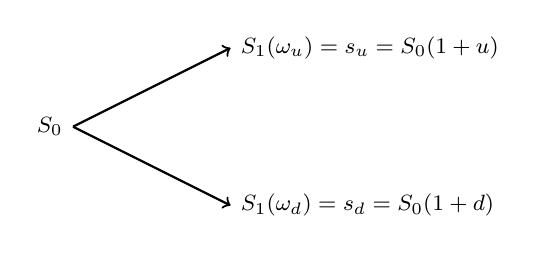
\begin{tikzpicture}
\draw[thick,->] (0,0) node[left] {\footnotesize $S_0$} 
  -- (2,1) node[right] {\footnotesize $S_1(\omega_u) = s_u = S_0(1+u)$};
\draw[thick,->] (0,0) 
  -- (2,-1) node[right] {\footnotesize $S_1(\omega_d) = s_d = S_0(1+d)$};
\end{tikzpicture}
\centering
\caption{Динамика цены акции в одношаговой модели.}
\label{os:f:price}  
\end{figure}

Таким образом, вся модель задается 4 параметрами $S_0,r,u,d$. Параметр $S_0$ положительный, а параметры $r$, $u$, $d$ больше $-1$.

\emph{Торговой стратегией} (или \emph{портфелем}) будем называть пару $\pi=(G,H)$, где $G$ выражает количество денежных единиц, вложенных в безрисковый актив, в момент времени $t=0$, а $H$ "--- количество акций, купленных в момент $t=0$.
Величины $G$ и $H$ могут быть как положительными, так и отрицательными (отрицательное количество денег означает взятие в долг, отрицательное количество акций -- короткую продажу); они также могут быть дробными. 

\emph{Стоимость портфеля $\pi$} сегодня по определению равна $V_0^\pi = G + HS_0$, а стоимость завтра равна $V_1^\pi(\omega) = G(1+r) + H S_1(\omega)$.
Изменение стоимости портфеля изображено на рис.~\ref{os:f:portfolio}.

\begin{figure}[h]
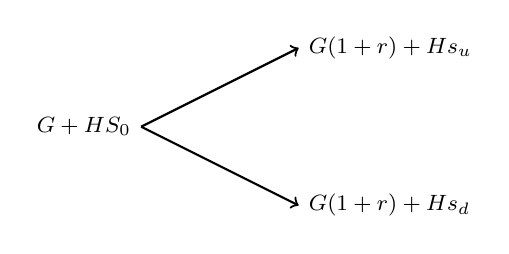
\begin{tikzpicture}
\draw[thick,->] (0,0) node[left] {\footnotesize $G+HS_0$} 
  -- (2,1) node[right] {\footnotesize $G(1+r) + Hs_u$};
\draw[thick,->] (0,0) --  (2,-1) node[right] {\footnotesize $G(1+r) + Hs_d$};
\end{tikzpicture}
\centering
\caption{Динамика стоимости портфеля в одношаговой модели.}
\label{os:f:portfolio}  
\end{figure}

\emph{Производный финансовый инструмент} (синоним -- \emph{платежное обязательство}) в такой модели представляется случайной величиной $X(\omega)$, которая задает сумму денег, которую \emph{продавец} этого инструмента выплачивает \emph{покупателю}%
\footnote{Названия сторон <<покупатель>> и <<продавец>> в такой абстрактной постановке весьма условны: если значение $X$ отрицательно, то, по сути, покупатель платит продавцу.}
в момент времени $t=1$. В свою очередь, покупатель покупает такой инструмент у продавца в момент времени $t=0$ за цену $V^X$.

Нашей задачей будет найти справедливую величину $V^X$.


\section{Цены платежных обязательств в одношаговой модели}

\subsection{Цена репликации}

\begin{definition}
Портфель $\pi$ \emph{реплицирует} платежное обязательство $X$, если $V_1^\pi(\omega) = X(\omega)$ для обоих исходов $\omega=\omega_u,\omega_d$. 
\end{definition}

\begin{proposition}
В одношаговой биномиальной модели для любого платежного обязательства существует единственный реплицирующий портфель.
\end{proposition}

\begin{proof}
Обозначим $x_u=X(\omega_u)$, $x_d=X(\omega_d)$.
Условие репликации эквивалентно системе линейных уравнений
\begin{equation}
\label{os:replication}
\left\{
\begin{aligned}
&G(1+r) + Hs_u = x_u,\\
&G(1+r) + Hs_d = x_d,
\end{aligned}\right.
\end{equation}
где $G$ и $H$ являются неизвестными.
В силу предположения $s_u>s_d$ решение этой системы существует и единственно.
\end{proof}

\begin{definition}
\emph{Ценой репликации} платежного обязательства $V^X$ называется стоимость $V^\pi_0$ соответствующего реплицирующего портфеля. 
\end{definition}

Найдем цену репликации в явном виде.
Решая систему \eqref{os:replication}, получаем, что реплицирующий портфель задается формулой
\label{os:replication-portfolio}
\[
G = \frac{1}{1+r} \cdot \frac{x_d s_u - x_us_d}{s_u - s_d}, \qquad
H = \frac{x_u-x_d}{s_u-s_d}.
\]
Теперь, учитывая, что $s_u = (1+u)S_0$, $s_d = (1+d)S_0$, находим
\[
V^X = G + HS_0 = \frac{1}{1+r}\cdot \frac{x_u(r-d) + x_d(u-r)}{u-d}.
\]

Как обсуждалось в первом разделе, цена репликации справедлива в том смысле, что она не приводит к возникновению арбитража (более точно, что такое арбитраж, мы определим далее). Поэтому естественно считать справедливой ценой платежного обязательства его цену репликации.


\subsection{Оценка с помощью риск-нейтральной вероятности}

Покажем, что цену репликации можно представить в виде математического ожидания относительно специально подобранной вероятности.

\begin{definition}
Вероятность $Q$ на множестве исходов $\Omega=\{\omega_u,\omega_d\}$ называется \emph{риск-нейтральной} если $Q(\omega_u) > 0$, $Q(\omega_d) > 0$ и $\E^Q {S_1}= (1+r)S_0$, где $\E^Q$ обозначает математическое ожидание по этой вероятности%
\footnote{То есть для случайной величины $\xi$ имеем $\E^Q \xi = \xi(\omega_u) Q(\omega_u) + \xi(\omega_d) Q(\omega_d)$.}.
\end{definition}

Название <<риск-нейтральная>> происходит из того, что цена акции сегодня будет равна ожиданию дисконтированной \emph{линейной полезности} от цены завтра по вероятности $\Q$: $S_0 = \E^Q u(S_1)/(1+r)$, где $u(x) = x$.
Экономические агенты, использующие линейную функцию полезности, считаются нейтральными к риску, что и объясняет название.

\begin{proposition}
\label{os:t:emm}
В одношаговой биномиальной модели риск-нейтральная вероятность существует тогда и только тогда, когда $d<r<u$.
Если она существует, то она единственна и задается формулой
\[
Q(\omega_u) = \frac{r-d}{u-d}, \qquad
Q(\omega_d) = \frac{u-r}{u-d}.
\]
\end{proposition}

\begin{proof}
Часть <<тогда>> и единственность $Q$ вытекают из того, что следующая система уравнений имеет единственное решение $(q_u,q_d)$ со строго положительными величинами $q_u$, $q_d$, которые соответствуют значениям $Q(\omega_u)$ и $Q(\omega_d)$:
\[
\left\{
\begin{aligned}
&(1+r)S_0 = s_dq_d + s_uq_u,\\
&q_u + q_d = 1.\\
\end{aligned}
\right.
\]
Первое уравнение здесь появляется из определения риск-нейтральной вероятности, а второе из того, что сумма вероятностей должна давать единицу.

Для доказательство части <<только тогда>> предположим, от противного, что $Q$ существует, но $r\le d < u$. Тогда
\[
\E^Q S_1 = s_d q_d + s_uq_u > (1+r)S_0 q_d + (1+r)S_0 q_u = (1+r)S_0.
\]
Наличие строго неравенства в этой формуле приводит к противоречию с определением $Q$.
Аналогично показывается, что и случай $d<u\le r$ невозможен.
\end{proof}

\begin{proposition}
Пусть $d < r< u$. Тогда для любого портфеля $\pi$ выполнено равенство
\[
V_0^\pi = \E^Q \frac{V_1^\pi}{1+r}.
\]
В частности, цену любого платежного обязательства $X$ можно найти как
\begin{equation}
\label{os:risk-neutal-price}
V^X = \E^Q \frac{X}{1+r}.
\end{equation}
\end{proposition}

\begin{proof}
Первое утверждение следует из цепочки равенств  
\[
\E^Q \frac{V_1^\pi}{1+r} = \E^Q \biggl(\frac{G(1+r) + HS_1}{1+r}\biggr) 
= G + H\E^Q\frac{S_1}{1+r} = G + HS_0 = V_0^\pi.
\]
Второе утверждение верно в силу того, что если портфель $\pi$ реплицирует $X$, то $X = V_1^\pi$ и $V^X = V_0^\pi$.
\end{proof}


\subsection{Отсутствие арбитража}

Рассмотрим подробнее условие $d<r<u$.
Оно означает, что доходность по безрисковому активу должна лежать строго между доходностью по акции в двух случаях $\omega_u$ и $\omega_d$.
Если это условие не выполнено, то инвестирование в один из активов оказывается заведомо менее прибыльным, чем в другой.
Покажем, что это приводит к арбитражу и, следовательно, в реалистичной модели всегда должно быть $d<r<u$.

\begin{definition}
\emph{Арбитражной возможностью} называется портфель $\pi$ со свойствами
\begin{alphenum}
\item $V_0^\pi = 0$,
\item $V_1^\pi(\omega) \ge 0$ для обоих исходов $\omega_u$, $\omega_d$,
\item $V_1^\pi(\omega) > 0$ хотя бы для одного из исходов $\omega_u$, $\omega_d$.
\end{alphenum}
\end{definition}
Первое условие означает, что для реализации арбитражной возможности не требуется начальных вложений капитала. Второе условие означает, что арбитражная возможность не несет риска. Третье условие "--- что она дает прибыль хотя бы в одном из исходов.

\begin{definition}
\emph{Гипотеза отсутствия арбитража NA} (no arbitrage) состоит в том, что в модели рынка нет арбитражных возможностей. 
\end{definition}

В финансовой математике считается, что во всех рассматриваемых моделях не должно быть арбитража, \te\ должна быть выполнена гипотеза NA.

\begin{proposition}
\label{os:ftap}
В одношаговой биномиальной модели выполнение гипотезы NA эквивалентно условию $d<r<u$, и, следовательно, эквивалентно существованию риск-нейтральной вероятности.
\end{proposition}

\begin{proof}
Пусть выполнено неравенство $d<r<u$. Тогда, согласно предложению \ref{os:t:emm}, существует риск-нейтральная вероятность $Q$.
Предположим, от противного, что существует арбитражная возможность $\pi$. Тогда 
\[
0 = V_0^\pi = \E^Q\frac{V_1^\pi}{1+r} 
= \frac{1}{1+r}( V_1^\pi(\omega_u) Q(\omega_u) + V_1^\pi(\omega_d) Q(\omega_d)) > 0.
\]
В последнем неравенстве воспользовались тем, что $V_1^\pi\ge 0$, причем хотя бы одно из значений $V_1^\pi(\omega_u)$ или $V_1^\pi(\omega_d)$ строго положительно, а кроме того обе вероятности $Q(\omega_u)$ и $Q(\omega_d)$ строго положительны.
Получаем противоречие: $0>0$.
Следовательно, арбитражная возможность не может существовать.

В обратную сторону: если $r\le d < u$, то нетрудно проверить, что $\pi = (-S_0,1)$ является арбитражной возможностью. Если же $d <u  \le r$, то $\pi = (S_0,-1)$ будет арбитражной возможностью.
В итоге, если арбитража нет, то должно быть выполнено неравенство $d<r<u$. 
\end{proof}

\begin{remark}
Предложение~\ref{os:ftap} является частным случаем \emph{первой фундаментальной теоремы финансовой математики}.
В общем виде она утверждает, что безарбитражность рынка равносильна существованию \emph{эквивалентной мартингальной меры}.
Для одношаговой биномиальной модели найденная нами риск"=нейтральная вероятность и есть такая мера. Общий случай мы обсудим позднее в курсе.
\end{remark}


\section{Примеры оценки платежных обязательств}

\subsection{Бескупонная облигация}
В одношаговой биномиальной модели \emph{бескупонная облигация}%
\footnote{В одношаговой модели нет смысла говорить о купонах, так как нет промежуточных моментов времени.}
соответствует платежному обязательству с константной выплатой $X$. 
Величина $X$ называется \emph{номиналом} (номинальной стоимостью) облигации.
Покажем, что цена такой облигации равна
\[
V^X = \frac{X}{1+r}.
\]

\textit{Первый способ (репликация).}
Выплату $X$ можно реплицировать портфелем $\pi=(G,H)$, где $G = X/(1+r)$ и $H=0$. Ясно, что $V^\pi_0 = G = X/(1+r)$.

\textit{Второй способ (риск-нейтральная оценка).}
По формуле \eqref{os:risk-neutal-price} имеем
\[
V^X = \E^Q \frac{X}{1+r} = \frac{X}{1+r},
\]
где воспользовались тем, что выражение под знаком ожидания есть константа.

\subsection{Форвардный контракт и форвардная цена}
По определению, \emph{форвардным контрактом} (или просто \emph{форвардом}) называется контракт на покупку базового актива по заранее установленной цене: покупатель форварда обязуется купить актив по цене $F$ в определенный момент времени, а продавец обязуется продать этот актив.

В одношаговой модели форвард соответствует платежному обязательству $X = S_1 - F$.
Так как в момент времени $t=0$ расчеты между сторонами не происходят, то  справедливое значение величины $F$ должно быть выбрано из условия $V^X=0$. Такое $F$ называется \emph{форвардной ценой} базового актива.
Покажем, что 
\[
F = (1+r) S_0.
\]

\textit{Первый способ (репликация).} Портфель $\pi=(G,H)$, где $G = -F/(1+r)$, $H=1$, реплицирует обязательство $X=S_1 - F$ для любого значения $F$. Начальная стоимость $V_0^\pi = S_0 - F/(1+r)$.
Тогда из условия $V^\pi_0 = 0$ находим $F=(1+r)S_0$.

\textit{Второй способ (риск-нейтральная оценка).} По формуле \eqref{os:risk-neutal-price} имеем
\[
V^X = \E^Q \frac{S_1 - F}{1+r} = \E^Q\frac{S_1}{1+r} - \frac{F}{1+r} = S_0 - \frac{F}{1+r},
\]
где во втором равенстве воспользовались определением риск-нейтральной вероятности ($\E^Q S_1/(1+r) = S_0$) и тем, что $F$ "--- константа.
Приравнивая $V^X_0$ к нулю, получаем такое же выражение для $F$, как и в способе с репликацией.

\subsection{Опционы колл и пут}
Европейские опционы колл и пут можно отождествить с платежными обязательствами
\[
X^c = (S_1 - K)^+, \qquad X^p = (K - S_1)^+,
\]
где запись $x^+$ означает $\max(x,0)$.
Действительно, если $S_1(\omega) > K$, то покупатель опциона колл получит выплату $S_1(\omega) - K$, а если $S_1(\omega) < K$, то выплаты не будет; кратко это можно записать как $(S_1 - K)^+$.
Аналогично для опциона пут.

Цены опционов вычисляются по формулам
\[
C =  \E^Q \frac{(S_1 - K)^+}{1+r}, \qquad
P = \E^Q \frac{(K - S_1)^+}{1+r}.
\]
Зная параметры модели, вычисление каждого из этих математических ожиданий сводится к вычислению суммы всего из двух слагаемых.

\subsection{Паритет цен колл"--~пут}
Пусть $C$ и $P$ "--- цены европейских опционов колл и пут на один и тот же базовый актив с одинаковым временем исполнения и одинаковым страйком.
Тогда справедливо равенство, называемое \emph{паритетом цен опционов колл и пут}:
\[
C - P = S_0 - \frac{K}{1+r}.
\]
Эквивалентно его можно записать также в виде
\[
C - P = B(F - K),
\]
где $B=1/(1+r)$ -- цена бескупонной облигации с номиналом 1, а $F=(1+r)S_0$ "--- форвардная цена.

Это равенство важно на практике. Например, с его помощью можно вычислить цену менее ликвидного опциона, зная цену более ликвидного; или зная цены обоих опционов, найти форвардную цену (о том, зачем это нужно, мы поговорим ближе к концу курса).

\textit{Доказательство с помощью репликации.} Рассмотрим портфель из одного опциона колл и минус одного опциона пут, \te\ по опциону колл мы выступаем покупателями, а по опциону пут продавцами%
\footnote{На финансовом языке можно было бы сказать, что по опциону колл у нас \emph{длинная} позиция, а по опциону пут \emph{короткая}.
Длинная позиция означает купленный контракт, а короткая "--- проданный.}.
Выплата по такому портфелю равна
\[
X = (S_1 - K)^+ - (K-S_1)^+ = S_1 - K,
\]
где воспользовались тем, что $x^+ - (-x)^+ = x$ для любого значения $x$.
Полученная выплата реплицируется одной единицей рискового актива и минус одной бескупонной облигацией с номиналом $K$.
В момент $t=0$ этот портфель стоит $S_0 - K/(1+r)$, откуда и следует доказываемое утверждение.

\textit{Доказательство с помощью риск-нейтральной оценки.} По формуле \eqref{os:risk-neutal-price} имеем цепочку равенств
\begin{equation}
\label{os:parity-proof}
C - P = \E^Q \frac{(S_1-K)^+ - (K -S_1)^+ }{1+r}
= \E^Q \frac{S_1 - K}{1+r} = S_0 - \frac{K}{1+r}.
\end{equation}


\summary

\begin{itemize}
\item Производными инструментами называются контракты, выплаты которых зависят от цен на базовые активы.

\item Основной принцип оценки производных инструментов: цена не должна вносить арбитраж на рынок.
Если возможна репликация выплаты производного инструмента, то стоимость реплицирующего портфеля является безарбитражной ценой. 

\item В одношаговой биномиальной модели любое платежное обязательство $X$ (производный инструмент) реплицируемо.
В случае $d<r<u$ его цена может быть найдена по формуле
\[
V^X = \E^{\Q} \frac{X}{1+r},
\]
где $Q(\omega_u) = \frac{r-d}{u-d}$, $Q(\omega_d) = \frac{u-r}{u-d}$ "--- риск-нейтральная вероятность.

\item Первая фундаментальная теорема финансовой математики утверждает, что отсутствие арбитража (гипотеза NA) равносильно существованию риск"=нейтральной вероятность; это, в свою очередь, равносильно условию $d<r<u$.

\item Цена бескупонной облигации с номиналом $X$: $B = X/(1+r)$.

\item Форвардная цена рискового актива: $F=(1+r)S_0$.

\item Паритет цен колл"--~пут: $C-P = S_0 - K/(1+r)$.
\end{itemize}

\chapter{Модель \crr}
\label{ch:crr}
\chaptertoc

Модель \crr\ (КРР) "--- это многошаговая биномиальная модель.
В отличие от одношаговой модели, в ней возникает задача динамической репликации, в которой реплицирующий портфель нужно ребалансировать с течением времени.
Модель КРР также интересна тем, что из нее в пределе можно получить известную модель \bs\ (см.\ дополнение \ref{ch:crr-limit}).

\section{Описание модели}
\subsection{Рисковый и безрисковый активы}

Рынок функционирует в моменты времени $t=0,1,\dots,T$.
Имеются два актива, \emph{безрисковый} и \emph{рисковый}. 

Безрисковый актив характеризуется постоянной процентной ставкой $r>-1$ за один период времени.
Сумма денег $x$ вложенная в него в момент $t$ превратится в $x(1+r)^s$ в момент $t+s$.
Удобно ввести последовательность цены безрискового актива 
\[
B_t = (1+r)^t.
\]
Можно, например, считать, что это цена бескупонной облигации со сроком погашения $T$ и номиналом $(1+r)^T$.
Номинал для удобства выбран так, чтобы начальная цена $B_0=1$.

Рисковый актив (например, акция) в начальный момент имеет константную цену $S_0>0$, а в каждый следующий момент его цена может измениться в $1+u$ или $1+d$ раз по сравнению с предыдущей ценой, где $-1<d<r<u$ "--- параметры модели.

Для описания случайного движения цены рискового актива введем пространство случайных исходов
\[
\Omega = \{\omega = (a_1,\dots,a_T) : a_t = 0\ \text{или}\ 1\}.
\]
Один исход $\omega$ задает всю траекторию цены от 0 до $T$. Если $a_t=1$, то цена идет <<вверх>> между моментами $t-1$ и $t$; если $a_t=0$, то цена идет <<вниз>>.
Заметим, что общее количество исходов в $\Omega$ равно $2^T$.
Рис.~\ref{crr:tree} дает качественное представление возможного движения цены в виде дерева.

\begin{figure}[h]
\centering
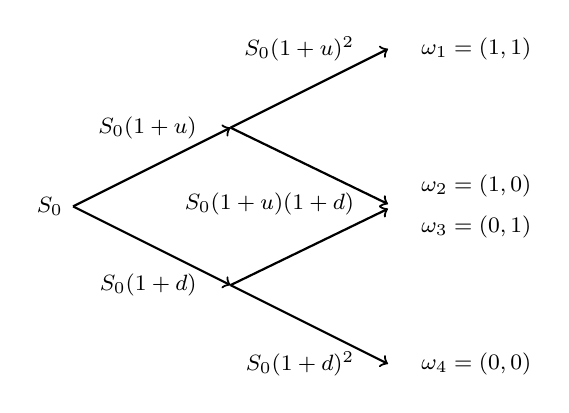
\begin{tikzpicture}
\draw[thick,->] (0,0) node[left] {\footnotesize $S_0$} 
  -- (2,1) node[left,xshift=-3mm] {\footnotesize $S_0(1+u)$};
\draw[thick,->] (0,0) 
  -- (2,-1) node[left,xshift=-3mm] {\footnotesize $S_0(1+d)$};

\draw[thick,->] (2,1) -- (4,2)  
  node[left,xshift=-3mm] {\footnotesize $S_0(1+u)^2$};
\draw[thick,->] (2,1) -- (4,0.03) 
  node[left,xshift=-3mm] {\footnotesize $S_0(1+u)(1+d)$};
\draw[thick,->] (2,-1) -- (4,-0.03);
\draw[thick,->] (2,-1) -- (4,-2) 
  node[left,xshift=-3mm] {\footnotesize $S_0(1+d)^2$};

\draw (4,2) node[xshift=3mm,right] {\footnotesize $\omega_1=(1,1)$};
\draw (4,0) node[xshift=3mm,above right] {\footnotesize $\omega_2=(1,0)$};
\draw (4,0) node[xshift=3mm,below right] {\footnotesize $\omega_3=(0,1)$};
\draw (4,-2) node[xshift=3mm,right] {\footnotesize $\omega_4=(0,0)$};
\end{tikzpicture}
\caption{Дерево для цены рискового актива в двухшаговой модели.}
\label{crr:tree}
\end{figure}

\begin{remark}
Формальное определение цены рискового актива в момент времени $t$ как функции от случайного исхода дается формулой
\[
S_t(\omega) = S_0 (1+u)^{\sum_{i=1}^t a_i} (1+d)^{t-\sum_{i=1}^t a_i}\ \text{для}\ \omega = (a_1,\dots,a_T).
\]
Показатель первой степени здесь равен количеству шагов вверх до момента $t$, а второй "--- количеству шагов вниз.
\end{remark}


\subsection{Торговые стратегии и условие самофинансируемости}

\emph{Торговой стратегией} будем называть последовательность $\pi_t=(G_t,H_t)$, $t=1,\dots,T$, где пара $(G_t,H_t)$ задает портфель активов, который покупается в момент времени $t-1$ и держится до момента $t$.
Величина $G_t$ выражает количество единиц безрискового актива в портфеле, а $H_t$ -- количество единиц рискового. 

Величины $G_t$, $H_t$ могут зависеть от рыночных цен рискового актива или, эквивалентно, от случайного исхода $\omega$.
Таким образом, мы считаем $G_t(\omega)$ и $H_t(\omega)$ случайными величинами, а $\pi_t(\omega)$ случайным вектором.
Как принято в теории вероятностей, указание зависимости от $\omega$ будет для краткости опускаться.

Следует учесть важное обстоятельство: портфель $\pi_t$, будучи купленным в момент $t-1$, не должен зависеть от цены рискового актива в последующие моменты времени.
Это можно сформулировать так: найдутся неслучайные функции $g_t$ и $h_t$ такие, что%
\footnote{Более подробно: $G_t(\omega) = g_t(S_0, S_1(\omega), \dots, S_{t-1}(\omega))$ и аналогично для $H_t$.
В следующей лекции мы узнаем, как можно более лаконично определить такую зависимость через понятие \emph{фильтрации}.}
$G_t=g_t(S_1,\dots,S_{t-1})$ и $H_t=h_t(S_1,\dots,S_{t-1})$.
При $t=1$ величины $G_1$ и $H_1$ не зависят от цен рискового актива и потому представляют собой константы%
\footnote{Заметим, что мы не говорим о зависимости от $S_0$, так как величина $S_0$ считается зафиксированной -- это цена рискового актива на рынке сейчас, она известна и неслучайна.}.

Эквивалентным образом, можно сказать, что случайные величины $G_t$ и $H_t$ должны обладать следующим свойством: для любых исходов $\omega = (a_1,\dots,a_T)$ и $\omega' = (a_1',\dots,a_T')$ таких, что $a_s = a_s'$ для всех $s=1,\dots,t-1$, выполнены равенства $G_t(\omega) = G_t(\omega')$ и $H_t(\omega) = H_t(\omega')$.

\begin{definition}
\emph{Стоимостью портфеля} стратегии $\pi$ в момент $t=1,\dots,T$ будем называть (случайную) величину
\[
V_t^\pi = G_tB_t + H_t S_t,
\]
а в момент $t=0$ (неслучайную) величину
\[
V_0^\pi = G_1 + H_1 S_0.
\]
\end{definition}

Таким образом, под стоимостью портфеля в момент $t$ понимается сумма денег, которую трейдер может выручить в момент времени $t$ от продажи портфеля $\pi_t$, который он купил в момент $t-1$. Так как в момент $t=0$ предыдущего портфеля не было, то мы полагаем $V_0^\pi$ равным стоимости первого портфеля%
\footnote{Может показаться, что здесь есть разногласие между формулами в нулевой момент времени и всеми остальными моментами.
Однако далее мы будем рассматривать только те стратегии, стоимость портфеля которых не меняется в течение торгов (см.~следующее определение). Для них имеет место равенство $V_t^\pi = G_{t+1}B_t + H_{t+1}S_t$ для всех $t=0,\dots,T-1$.}.

Следующее определение вводит важный класс стратегий, у которых нет притока или оттока капитала извне.
Только такие стратегии будут рассматриваться в задаче репликации платежных обязательств при определении их цен.

\begin{definition}
Стратегия $\pi$ называется \emph{самофинансируемой}, если для всех $t=1,\dots,T-1$ выполняется равенство
\begin{equation}
\label{crr:sf}
(H_{t+1} - H_t)S_t = -(G_{t+1} - G_t)B_t.
\end{equation}
\end{definition}
Смысл равенства \eqref{crr:sf} состоит в том, что изменение стоимости позиции по рисковому активу должно в точности покрываться изменением стоимости позиции по безрисковому активу (\te\ купить рисковый актив можно только за счет продажи безрискового, и наоборот). 
Считается, что торговля происходит в моменты $t=0,\dots,T$, причем в течение торгов цены активов остаются зафиксированными, однако они изменяются между моментами торгов. Таким образом, изменение стоимости портфеля может происходить только за счет изменения цен активов, и, следовательно, у самофинансируемой стратегии отсутствует приток или отток капитала.

\begin{remark}
Равенство \eqref{crr:sf} можно также записать в виде
%\begin{equation}
%\label{crr:sf-2}
\[
G_tB_t + H_tS_t = G_{t+1}B_t + H_{t+1}S_t, \qquad t=1,\dots,T-1,
\]
%\end{equation}
что имеет следующий смысл: стоимость портфеля $\pi_t$, с которым мы начинаем торги в момент времени $t$, равна стоимости портфеля $\pi_{t+1}$, с которым мы заканчиваем торги.
Опять-таки, это означает, что нет притока и оттока капитала.
\end{remark}

% Из определения стоимости портфеля и равенства \eqref{crr:sf-2} сразу следует удобная эквивалентная форма условия самофинансируемости: для $t=0,\dots,T-1$ должно быть выполнено равенство
% \begin{equation}
% \label{crr:sf-equiv}
% V_t^\pi = G_{t+1}B_t + H_{t+1}S_t.
% \end{equation}

Докажем одно полезное представление для стоимости портфеля самофинансируемой стратегии, которое далее будет часто использоваться.

\begin{proposition}
\label{crr:p:sf-value}
Для любой самофинансируемой стратегии верно равенство
\begin{equation}
\label{crr:sf-value}
V_t^\pi = V_0^\pi + \sum_{s=1}^t (G_u \Delta B_u + H_u\Delta S_u),
\end{equation}
где $\Delta B_u = B_u - B_{u-1}$, $\Delta S_u = S_u - S_{u-1}$ обозначают изменения цен за период.
\end{proposition}
Интерпретация формулы \eqref{crr:sf-value}: в момент времени $t$ стоимость портфеля самофинансируемой стратегии складывается из начальной стоимости портфеля и суммы изменений стоимости за каждый шаг до момента $t$.
\begin{proof}
Докажем по индукции.
Для $t=0$ утверждение, очевидно, верно.
Если оно верно для $t$, то представим
\begin{multline*}
V_{t+1}^\pi = G_{t+1}B_{t+1} + H_{t+1}S_{t+1} 
= (G_{t+1}B_{t} - G_tB_t + H_{t+1}S_t - H_tS_t)
\\+ (G_tB_t + H_tS_t) + (G_{t+1}\Delta B_{t+1} + H_{t+1}\Delta S_{t+1})
\end{multline*}
(во втором равенство просто добавили и вычли одинаковые слагаемые).
Первая скобка в правой части равна 0 по условию самофинансирования, а вторая скобка равна $V_t^\pi$ по определению стоимости портфеля.
Таким образом,
\[
V_{t+1}^\pi = V_t^\pi + G_{t+1}\Delta B_{t+1} + H_{t+1}\Delta S_{t+1},
\]
откуда следует справедливость шага индукции.
\end{proof}


\subsection{Платежные обязательства}

\begin{definition}
\emph{Платежным обязательством европейского типа} называется контракт между покупателем и продавцом, согласно которому продавец платит покупателю сумму денег $X(\omega)$ в момент времени $T$. 
\end{definition}

Далее все рассматриваемые платежные обязательства будут европейскими, поэтому словосочетание <<европейского типа>> будет опускаться. 


В качестве примера платежных обязательств, можно привести опционы колл и пут с функциями выплат $X^\text{call} = (S_T- K)^+$, $X^\text{put} = (K-S_T)^+$, где $K$ -- цена страйк. Заметим, что выплата $X$ является случайной величиной, причем она может зависеть от всей траектории цены рискового актива, а не только от его цены в последний момент времени.

Нашей следующей задачей будет определить понятие цены платежного обязательства.
Это будет сделано по аналогии с одношаговой моделью: мы покажем, что любое платежное обязательство имеет единственную реплицирующую стратегию, и, следовательно, стоимость портфеля этой стратегии и будет справедливой (безарбитражной) ценой платежного обязательства.


\section{Репликация платежных обязательств}
\subsection{Метод обратной индукции}

В модели КРР цену репликации любого платежного обязательства и реплицирующую стратегию можно найти с помощью \emph{метода обратной индукции}.
Мы сначала сформулируем теорему и рассмотрим конкретный пример, который поможет понять суть доказательства.
Само доказательство приводится в следующем разделе.

\begin{theorem}
В модели КРР для любого платежного обязательства $X$ существует единственная самофинансируемая стратегия $\pi$, называемая \emph{реплицирующей стратегией}, такая, что $V_T^\pi(\omega) = X(\omega)$ для всех $\omega$.
\end{theorem}

\begin{definition}
\emph{Ценой репликации} $V_t^X$ платежного обязательства $X$ в момент времени $t\le T$ называется стоимость портфеля реплицирующей стратегии, \te\ $V_t^X = V_t^\pi$.
\end{definition}

\begin{example}
\label{crr:example}
Рассмотрим двухшаговую модель ($T=2$) с параметрами $S_0=100$, $u=0.1$, $d=-0.1$, $r=0.05$.
Найдем цену репликации опциона колл с временем исполнения $T=2$ и страйком $K=100$.

Будем двигаться назад по моментам времени $t=2,1,0$.
Для $t=2$ цена $V_2^X$ должна равняться $X$, так как если платежное обязательство производит выплату сразу в момент покупки, то его цена равна этой выплате.
Для нашего опциона $X(\omega_1) = 21$ и $X(\omega_i) = 0$, $i=2,3,4$.

В момент $t=1$ имеется две ситуации: цена рискового актива может быть 110 или 90.
В первом случае мы знаем, что в следующий момент времени нам нужно произвести выплату 21 или 0 в зависимости от того, куда пойдет цена.
Из результатов для одношаговой модели, найдем реплицирующий портфель и его стоимость.
Для этого нужно решить систему
\begin{equation}
\label{crr:example-system}
\left\{
\begin{aligned}
&G_2 B_2 + H_2 S_2(\omega_1) = X(\omega_1), \\
&G_2 B_2 + H_2 S_2(\omega_2) = X(\omega_2)
\end{aligned}
\right. \implies
\left\{
\begin{aligned}
&1.05^2 G_2  + 121 H_2 = 21, \\
&1.05^2 G_2 +  99 H_2 = 0.
\end{aligned}
\right.
\end{equation}
Находим $G_2 \approx 85.71$, $H_2 \approx 0.95$ и отсюда получаем стоимость реплицирующего портфеля в момент $t=1$ при цене рискового актива 110: $V_1^X(\omega_1) = V_1^X(\omega_2) = 1.05 G_2 + 110 H_2 = 15$.

Заметим, что если искать компоненты реплицирующей стратегии не требуется, а нужно найти лишь цену репликации, то можно воспользоваться следующей формулой, вытекающей из риск-нейтральной оценки для одношаговой модели:
\begin{equation}
\label{crr:example-step}
V_1(\omega_1) = \frac{21 \cdot q + 0\cdot (1-q)}{1+r} = 15,
\end{equation}
где $q = \frac{r-d}{u-d} = \frac34$ -- риск-нейтральная вероятность. 

Аналогично рассматривается ситуация, когда цена рискового актива в момент $t=1$ равна 90. В этом случае $G_2=H_2 = 0$, $V_1 = 0$ (в следующий момент выплата нулевая).

Наконец, переходим к моменту $t=0$. Нам достаточно построить портфель, который в момент $t=1$ будет стоить $V_1^X$ и в случае, когда цена пойдет вверх, и в случае, когда цена пойдет вниз. 
Если мы найдем такой портфель, то его стоимости будет достаточно, чтобы преобразовать его в уже построенный реплицирующий портфель в момент $t=1$.
Получаем систему, аналогичную \eqref{crr:example-system}:
\[
\left\{
\begin{aligned}
&1.05 G_1  + 110 H_1 = 15, \\
&1.05 G_1 +  90 H_1 = 0.
\end{aligned}
\right.
\]
Решение: $G_1\approx -64.29$, $H_1=3/4$, откуда $V_0^X = G_1 + 100 H_1 \approx 10.71$.
Задача решена.
\end{example}

\begin{remark}
Процесс нахождения цены репликации удобно изображать графически в виде процедуры последовательного заполнения таблицы для значений $V_t$ с конца, см.~рис.~\ref{crr:replication}. 
Сначала нужно составить таблицу цен рискового актива и выплаты опциона (верхняя таблица на рисунке).
Затем положить $V_2=X_2$ (первая таблица во втором ряду). Чтобы найти $V_1$, воспользуемся формулой для риск-нейтральной цены в одношаговой модели (см.~формулу~\eqref{crr:example-step}; в общем случае нужно использовать формулу \eqref{crr:v-by-backward-induction} далее).
Аналогичные вычисления проделываем для $V_0$.

\begin{figure}[h]
\centering
\begin{tabular}{r|ccc|c}
& $S_0$ & $S_1$ & $S_2$ & $X$ \\\hline
$\omega_1$ & 100 & 110 & 121 & 21 \\
$\omega_2$ & 100 & 110 & 99 & 0 \\
$\omega_3$ & 100 & 90 & 99 & 0 \\
$\omega_4$ & 100 & 90 & 81 & 0 \\
\end{tabular}
%
\\[2em]
%
\begin{tabular}{r|ccc}
& $V_0$ & $V_1$ & $V_2$  \\\hline
$\omega_1$ & $\boldsymbol\cdot$ & $\boldsymbol\cdot$  & 21 \\
$\omega_2$ & $\boldsymbol\cdot$ & $\boldsymbol\cdot$  & 0 \\
$\omega_3$ & $\boldsymbol\cdot$ & $\boldsymbol\cdot$  & 0 \\
$\omega_4$ & $\boldsymbol\cdot$ & $\boldsymbol\cdot$  & 0 \\
\end{tabular}
%
$\implies$
%
\begin{tabular}{r|ccc}
& $V_0$ & $V_1$ & $V_2$  \\\hline
$\omega_1$ & $\boldsymbol\cdot$ & 15  & 21 \\
$\omega_2$ & $\boldsymbol\cdot$ & 15  & 0 \\
$\omega_3$ & $\boldsymbol\cdot$ & 0  & 0 \\
$\omega_4$ & $\boldsymbol\cdot$ & 0  & 0 \\
\end{tabular}
%
$\implies$
%
\begin{tabular}{r|ccc}
& $V_0$ & $V_1$ & $V_2$  \\\hline
$\omega_1$ & 10.71 & 15  & 21 \\
$\omega_2$ & 10.71 & 15  & 0 \\
$\omega_3$ & 10.71 & 0  & 0 \\
$\omega_4$ & 10.71 & 0  & 0 \\
\end{tabular}\\[1em]
\caption{Расчет цены опциона с помощью обратной индукции.}
\label{crr:replication}
\end{figure}
\end{remark}


\subsection{\difficult\ Доказательство теоремы}
\textit{Шаг 1 (построение).}
Определим случайные величины $V_t$ для $t=T,\,T-1,\ldots,0$ и $G_t$, $H_t$ для $t=T,\ldots,1$, где $V_t$ будет играть роль цены платежного обязательства или стоимости реплицирующего портфеля, а $G_t$ и $H_t$ "--- роль количества активов в портфеле реплицирующей стратегии.

Для $t=T$ положим $V_T = X$.
Если случайная величина $V_t$ определена, то в качестве $V_{t-1}(\omega)$ для $\omega=(a_1,\dots,a_T)$ возьмем цену репликации в одношаговой биномиальной модели платежного обязательства с выплатой
\[
\tilde X(\omega_u) = V_{t}(a_1,\ldots,a_{t-1}, 1), \qquad
\tilde X(\omega_d) = V_{t}(a_1,\ldots,a_{t-1}, 0),
\]
а значения $G_{t}(\omega)$ и $H_{t}(\omega)$ зададим как решения уравнений 
\begin{equation}
\label{crr:replication-step}
\left\{
\begin{aligned}
&G_t B_t + H_t S_t(a_1,\ldots,a_{t-1}, 1) = V_{t}(a_1,\ldots,a_{t-1}, 1),\\
&G_t B_t + H_t S_t(a_1,\ldots,a_{t-1}, 0) = V_{t}(a_1,\ldots,a_{t-1}, 0).
\end{aligned}
\right.
\end{equation}
Решение системы существует и единственно в силу различия величин $S_t(\ldots, 1)$ и $S_t(\ldots,0)$.
В явном виде имеем
\begin{equation}
\label{crr:v-by-backward-induction}
V_{t-1}(\omega) 
= \frac
  {V_t(a_1,\ldots,a_{t-1}, 1)\cdot q + V_t(a_1,\ldots,a_{t-1}, 0)\cdot (1-q)}
  {1+r} ,
\end{equation}
где $q= \frac{r-d}{u-d}$ -- риск-нейтральная вероятность.
Продолжая по индукции, построим указанные последовательности для всех $t$. 

Отметим, что величины $V_t(\omega)$ зависят только от компонент $a_1,\ldots,a_t$ случайного исхода $\omega=(a_1,\dots,a_T)$, а величины $G_t(\omega)$, $H_t(\omega)$ зависят только от компонент $a_1,\ldots,a_{t-1}$.
В частности, отсюда следует, что последовательность $\pi_t=(G_t,H_t)$ задает торговую стратегию.

\textit{Шаг 2 (проверка).} Покажем, что $V_t^\pi = V_t$, причем $\pi$ является самофинансируемой стратегией и реплицирует $X$.
Заметим, что система \eqref{crr:replication-step} означает равенство
\begin{equation}
\label{crr:replication-value-1}
V_t = G_tB_t + H_t S_t.
\end{equation}
Кроме того, находя в явном виде $G_t$ и $H_t$ и используя \eqref{crr:v-by-backward-induction}, нетрудно проверить, что 
\begin{equation}
\label{crr:replication-value-2}
V_{t-1} = G_tB_{t-1} + H_t S_{t-1}.
\end{equation}
Из равенства \eqref{crr:replication-value-1} следует, что $V_t = V_t^\pi$ для всех $t\ge 1$, а из равенства \eqref{crr:replication-value-2} следует, что $V_0 = V_0^\pi$.
Итак, $V_t^\pi = V_t$ для всех $t=0,\dots,T$.
Из равенств \eqref{crr:replication-value-1} и \eqref{crr:replication-value-2} также нетрудно видеть, что выполнено условие самофинансируемости.
Так как $V_T^\pi = V_T=X$, то $\pi$ реплицирует $X$.

\textit{Шаг 3 (единственность).} Из единственности решения системы \eqref{crr:v-by-backward-induction} следует, что цена репликации определена однозначно.
Тогда единственность реплицирующей стратегии следует из того, если $\pi_t=(G_t,H_t)$ "--- реплицирующая стратегия, то для каждого $t$ и каждого набора $(a_1,\dots,a_{t-1})$ должна быть выполнены равенства
\[
\left\{
\begin{aligned}
&G_t(a_1,\dots,a_{t-1}) B_t + H_t(a_1,\dots,a_{t-1}) S_t(a_1,\ldots,a_{t-1}, 1) = V_{t}(a_1,\ldots,a_{t-1}, 1),\\
&G_t(a_1,\dots,a_{t-1}) B_t + H_t(a_1,\dots,a_{t-1}) S_t(a_1,\ldots,a_{t-1}, 0) = V_{t}(a_1,\ldots,a_{t-1}, 0).
\end{aligned}
\right.
\]
Решение этой системы относительно $G_t,H_t$ единственно.


\section{Риск-нейтральная оценка}

Покажем, что, аналогично одношаговой модели, цены платежных обязательств могут быть вычислены как ожидания дисконтированной выплаты\footnote{Дисконтированной выплатой называется величина $X/B_T$.} по риск-ней\-траль\-ной вероятности. 

Определим риск-нейтральную вероятность в модели КРР по формуле
\[
Q(\omega) = q^{\sum_{i=1}^T a_i} (1-q)^{T-\sum_{i=1}^T a_i}\ \text{для}\ \omega = (a_1,\dots,a_T),
\]
где $q = \frac{r-d}{u-d}$ есть риск-нейтральная вероятность в одношаговой модели.
Таким образом, $Q(\omega)$ приписывает траектории цены рискового актива вероятность пойти вверх на каждом шаге равную $q$ и вероятность пойти вниз $1-q$. 

\begin{example}
Риск-нейтральная вероятность в двухшаговой модели изображена на рис.~\ref{crr:fig:risk-neutral}. Для модели из примера~\ref{crr:example} имеем $q=3/4$, и, следовательно, $Q(\omega_1)=q^2 = 9/16$, $Q(\omega_2)=Q(\omega_3)=q(1-q) = 3/16$, $Q(\omega_4)=(1-q)^2 = 1/16$.

\begin{figure}[h]
\centering
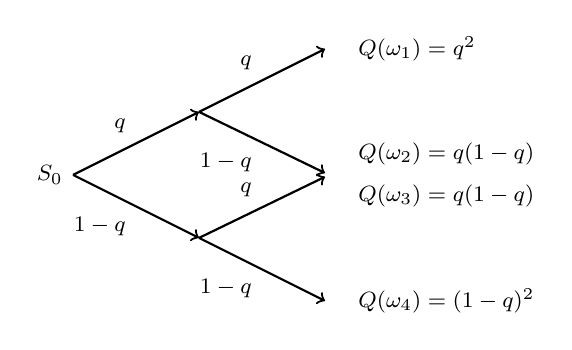
\begin{tikzpicture}[scale=0.8]
\draw[thick,->] (0,0) node[left] {\footnotesize $S_0$} 
  --node[midway,above left] {\footnotesize $q$} (2,1);
\draw[thick,->] (0,0) 
  --node[midway,below left] {\footnotesize $1-q$} (2,-1);

\draw[thick,->] (2,1) --node[midway,above left] {\footnotesize $q$} (4,2);
\draw[thick,->] (2,1) -- node[midway,below left] {\footnotesize $1-q$} (4,0.03);
\draw[thick,->] (2,-1) --node[midway,above left] {\footnotesize $q$} (4,-0.03);
\draw[thick,->] (2,-1) --node[midway,below left] {\footnotesize $1-q$} (4,-2);

\draw (4,2) node[xshift=3mm,right] {\footnotesize $Q(\omega_1)=q^2$};
\draw (4,0) node[xshift=3mm,above right] {\footnotesize $Q(\omega_2)=q(1-q)$};
\draw (4,0) node[xshift=3mm,below right] {\footnotesize $Q(\omega_3)=q(1-q)$};
\draw (4,-2) node[xshift=3mm,right] {\footnotesize $Q(\omega_4)=(1-q)^2$};
\end{tikzpicture}
\caption{Риск-нейтральная вероятность в двухшаговой модели.}
\label{crr:fig:risk-neutral}
\end{figure}
\end{example}

\begin{theorem}
Для цены репликации платежного обязательства $X$ в начальный момент времени%
\footnote{Аналогичная формула будет верна и для цены в промежуточные моменты времени, но чтобы ее записать, нам потребуется понятие условного математического ожидания.
Мы изучим его в следующей лекции.} справедлива формула
\[
V_0^X = \E^Q\left(\frac{X}{B_T}\right) \qquad \left(\;= (1+r)^{-T} \E^Q X\right).
\]
\end{theorem}

\begin{proof}[Доказательство \difficult]
Воспользуемся индукцией по количеству периодов $T$.
Для $T=1$ утверждение верно из результатов для одношаговой модели. 

Пусть $\Omega'$ и $Q'$ обозначают пространство случайных исходов и риск"=нейтральную вероятность в модели с $T-1$ периодами. 
Так как реплицирующая стратегия для $X$ также может реплицировать платежное обязательство с выплатой $X'=V_{T-1}^X$ в момент $T-1$, то из предположения индукции имеем
\[
V_0^X = \E^{Q'}\left(\frac{V_{T-1}^X}{B_{T-1}}\right).
\]
Из риск-нейтральной оценки для одношаговой модели находим
\[
V_{T-1}^X(\omega') = \frac{1}{1+r}(q X(\omega_u') + (1-q) X(\omega_d')),
\]
где $\omega' = (a_1,\ldots,a_{T-1})$ и $\omega'_u = (a_1,\ldots,a_{T-1},1)$, $\omega'_d = (a_1,\ldots,a_{T-1},0)$.
Теперь доказываемое утверждение следует из цепочки равенств
\begin{multline*}
V_0^X = \sum_{\omega'\in\Omega'} 
  \frac{V_{T-1}^X(\omega')}{{B_{T-1}}} Q'(\omega') \\
= \sum_{\omega'\in\Omega'} \frac{1}{(1+r)B_{T-1}}
  \left(X(\omega'_u) q Q'(\omega') + X(\omega'_d) (1-q) Q'(\omega')\right) \\
=  \sum_{\omega\in\Omega} \frac{1}{B_T} X(\omega) Q(\omega) 
= \E^Q\left(\frac{X}{B_T}\right),
\end{multline*}
где во втором равенстве воспользовались тем, что сумму по $\omega'\in \Omega'$ во второй строке можно разбить на две (в одной будут слагаемые с $X(\omega'_u)$, а в другой с $X(\omega'_d)$), а затем перегруппировать слагаемые таким образом, чтобы получить одну сумму по $\omega\in\Omega$.
\end{proof}

\begin{corollary}
\label{crr:martingale}
Для любого $t$ справедливо равенство $S_0 = (1+r)^{-t}\E^Q S_t$.
\end{corollary}
\begin{proof}
Платежное обязательство с выплатой $X=S_t$ в момент $t$ реплицируется портфелем из одной акции (\te\ $\pi_t\equiv(0,1))$, стоимость которого в начальный момент времени равна $S_0$.
С другой стороны, эта же стоимость является ценой репликации, которая по теореме равна $(1+r)^{-t}\E^Q S_t$.
\end{proof}


\section{Примеры оценки платежных обязательств}

\subsection{Бескупонная облигация}
Бескупонная облигация с временем погашения $T$ соответствует платежному обязательству с константой выплатой $X$ (\emph{номиналом} облигации) в момент $T$.
Ее цена задается формулой
\[
V_t^X = (1+r)^{t-T}X.
\]
Это выражение следует из того, что такая облигация реплицируется постоянным портфелем $\pi_t\equiv(G,0)$ с $G = (1+r)^{-T} X$.
Для $t=0$, мы также можем воспользоваться риск-нейтральной оценкой: $V_0^X = (1+r)^{-T} \E^Q X = (1+r)^{-T} X$.

\subsection{Форвардная цена}
\emph{Форвардной ценой} (более точно, $T$-форвардной ценой) рискового актива в момент времени $t=0$ называется (неслучайная) величина $F$ такая, что контракт на покупку актива по цене $F$ в момент времени $t=T$ имеет нулевую стоимость в момент $t=0$. 

Рассматривая платежное обязательство $X=S_T-F$ и приравнивая $V^X_0 = 0$, получаем уравнение
$(1+r)^{-T} \E^Q (S_T - F) = 0$.
Пользуясь следствием~\ref{crr:martingale}, находим $F= (1+r)^T S_0$.

Этот результат можно получить и с помощью репликации.
Действительно, выплата $X=S_T-F$ реплицируется портфелем из одной акции и минус одной бескупонной облигации с номиналом $F$.
В начальный момент стоимость такого портфеля равна $S_0 - (1+r)^{-T} F$.
Нулевую стоимость дает $F = (1+r)^T S_0$.

\subsection{Платежные обязательства, не зависящие от траектории цены}
Если платежное обязательство $X = f(S_T)$ зависит только от цены рискового актива в последний момент времени (как, например, у ванильных опционов), то можно воспользоваться тем, что $S_T$ представима в виде
\[
S_T = S_0 (1+u)^\xi(1+d)^{T-\xi},
\]
где величина $\xi$ равна количеству шагов цены вверх на всей траектории.
Относительно риск-нейтральной вероятности $\xi$ имеет биномиальное распределение с параметрами $T$ и $q$.
Тогда цену репликации можно записать в виде ожидания по биномиальному распределению, что дает формулу
\[
V_0^X = (1+r)^{-T} \sum_{n=0}^T f\left(S_0 (1+u)^n(1+d)^{T-n}\right) \cdot C_T^n q^n (1-q)^{T-n}.
\]

\subsection{Платежные обязательства, зависящие от траектории цены}
Если выплата зависит от всей траектории цены, то воспользоваться формулой с биномиальным распределением не получится, и нужно явно найти риск-нейтральную вероятность каждой траектории и выплату на этой траектории.

\begin{example}
\label{crr:e:barrier}
Рассмотрим двухшаговую модель с параметрами из примера \ref{crr:example} и вычислим в ней цену \emph{барьерного опциона вниз-и-выход} колл с со страйком $K=95$ и барьером $H=92$. Этот опцион разрешается исполнить только если его цена за все моменты времени не опустится ниже $H$.
Выплата имеет следующий вид
\[
X(\omega_1) = 26, \quad X(\omega_2) = 4, \quad X(\omega_3) = X(\omega_4)=0.
\]
Используя риск-нейтральные вероятности исходов из примера \ref{crr:example}, получаем
\[
V_0^X = \frac1{1.05^2}\left(26 \cdot \frac9{16} + 4\cdot \frac3{16}\right) \approx 13.95.
\]
\end{example}

\begin{remark}
К сожалению, подобный метод вычисления становится слишком трудоемким при увеличении числа шагов в модели, так как число траекторий растет экспоненциально.
Тем не менее, часто получается упростить задачу, если выплата $X$ задается функцией от некоторой  случайной последовательности, обладающей марковским свойством (но мы не будем касаться этого подхода). 

Другой способ заключается в симуляции траекторий моделей и вычислении математического ожидания в формуле для цены платежного обязательства с помощью метода Монте-Карло.
Мы подробно рассмотрим метод Монте-Карло для модели \bs\ в лекции \ref{ch:mc}; большинство рассуждений оттуда можно перенести и на модель \crr.
\end{remark}

\subsection{Паритет цен колл"--~пут}
Аналогично одношаговой биномиальной модели, в модели КРР справедливо равенство 
\[
C-P = S_0 - \frac{K}{B_T} \quad (= S_0 - K(1+r)^{-T}),
\]
где $C$ и $P$ "--- цены (в момент времени 0) европейских опционов колл и пут со одинаковым страйком $K$ и временем исполнения $T$.
Доказательство аналогично формуле \eqref{os:parity-proof} в лекции \ref{ch:onestep}:
\[
C - P = \E^Q \frac{(S_T-K)^+ - (K-S_T)^+ }{B_T}
= \E^Q \frac{S_T - K}{B_T} = S_0 - \frac{K}{B_T}.
\]
Можно также дать доказательство через репликацию выплаты длинной позиции по опциону колл и короткой позиции по опциону пут с помощью бескупонной облигации и рискового актива (упражнение). 


\summary

\begin{itemize}
\item В модели \crr\ (многошаговой биномиальной модели) безрисковый актив имеет цену $B_t=(1+r)^t$, а цена рискового актива на каждом шаге может изменяться в $1+u$ или $1+d$ раз, где $d<r<u$.

\item Любое платежное обязательство $X$ реплицируемо.
Реплицирующую стратегию можно найти методом обратной индукции.
Цену репликации в момент $t=0$ можно найти по формуле
\[
V^X_0 = \E^{\Q} \frac{X}{B_T},
\]
где $\Q$ "--- риск-нейтральная вероятность, относительно которой цена рискового актива идет вверх с вероятностью $q_u = \frac{r-d}{u-d}$ и вниз с вероятностью $q_d = \frac{u-r}{u-d}$.

\item Цена бескупонной облигации с номиналом $X$: $B = X/(1+r)^T$.

\item Форвардная цена рискового актива: $F=(1+r)^TS_0$.

\item Паритет цен пут"--~колл: $C-P = S_0 - K/B_T$.
\end{itemize}

%!TEX root=finmath1.tex
\chapter{Мартингалы}
\label{ch:mart}
\chaptertoc

Мартингал "--- это случайная последовательность (или процесс) такая, что математическое ожидание ее будущих значений равно текущему значению.

В финансовой математике мартингалы играют чрезвычайно важную роль, потому что при отсутствии арбитража дисконтированные цены активов должны являться мартингалами относительно так называемых эквивалентных мартингальных мер (это обобщение понятия риск-нейтральной вероятности).

Чтобы ввести понятие мартингала нам потребуются понятия условного математического ожидания и фильтрации на вероятностном пространстве, с которых мы и начнем эту лекцию.

Почти все результаты будут приведены без доказательств.
Их можно найти, например, в книге \cite{Shiryaev04} (см.~главу II.7 об условном математическом ожидании и главу VII.1 о мартингалах).


\section{Условное математическое ожидание}
\subsection{Подготовительные рассуждения}

Определение условного математического ожидания в полной общности может показаться слишком абстрактным, поэтому начнем с частных случаев.

Для начала рассмотрим вероятностное пространство с конечным множеством исходов.
Без ограничения общности будет считать, что вероятности всех исходов строго положительны. Случайные величины на таком пространстве принимают конечное число значений.

Если $X$ "--- случайная величина, а $A$ "--- случайное событие, то определим условное математическое ожидание $X$ при условии $A$ по формуле
\[
\E(X\mid A) = \sum_{i=1}^n x_i \P(X=x_i\mid A),
\]
\te\ заменив в определении математического ожидания обычные вероятности на условные. 
Интерпретировать $\E(X\mid A)$ можно как среднее значение величины $X$ в случае, когда мы знаем, что произошло событие $A$.

Пусть теперь $X$ и $Y$ "--- две случайные величины.
Если значение $Y$ известно, то вычислить условное ожидание $X$, учитывая эту информацию, можно как $\E(X\mid Y=y)$, где ``$Y=y$'' означает соответствующее случайное событие.
Имея это ввиду, определим условное ожидание $X$ при условии $Y$ как
\[
\E(X\mid Y) = g(Y),\ \text{где}\ g(y) = \E(X\mid Y=y).
\]
Отметим, что, по определению, $\E(X\mid Y)$ само является случайной величиной.
Это удобно, в частности, потому что позволяет применять к нему те же операции, что и к обычным случайным величинам.

Нетрудно показать, что условное ожидание обладает следующими свойствами.
Если $X,Y,Z$ "--- случайные величины, а $f(y)$ "--- произвольная функция, то 
\begin{align*}
&\E(X+Z \mid Y) = \E(X\mid Y) + \E(Z\mid Y),\\
&\E(f(Y)X \mid Y) = f(Y)\E(X\mid Y),\\
&\E(\E(X\mid Y)) = \E X.
\end{align*}
Первое свойство "--- это линейность условного ожидания.
Второе свойство "--- более сильная форма линейности, которая позволяет выносить из условного ожидания множители, функционально зависящие от $Y$ (как из обычного ожидания можно выносить константы).
Третье свойство означает, что условное ожидание дает несмещенную оценку для обычного ожидания%
\footnote{Понятие несмещенной оценки вводится в курсе математической статистики.
Дальше оно нам не потребуется.}.

В качестве следствия из второго и третьего равенств получаем, что 
\begin{equation}
\label{mart:defining-property}
\E(f(Y)X) = \E(f(Y)\E(X\mid Y)).
\end{equation}
Оказывается, формула \eqref{mart:defining-property} является определяющим свойством условного ожидания в следующем смысле: для любых случайных величин $X,Y$ (пока все еще на конечном вероятностном пространстве), существует единственная случайная величина $U$ (а именно, $U=\E(X\mid Y)$) такая, что она может быть представлена в виде $U=g(Y)$, и для любой функции $f(y)$ выполнено
\[
\E(f(Y)X) = \E(f(Y)U).
\]

Используя эту идею, распространим понятие $\E(X\mid Y)$ на произвольные вероятностные пространства.
Конструкция дается в два этапа: сначала для неотрицательных $X$, а потом для произвольных.

Можно показать, что для случайной величины $X\ge 0$ и произвольной случайной величины $Y$ найдется п.н.-единственная расширенная\footnote{То есть может принимать значение $+\infty$} величина $U\ge0$ такая, что $U=g(Y)$, и для любой неотрицательной функции $f(y)$ выполнено равенство
\[
\E(f(Y)X) = \E(f(Y)U).
\]
Тогда положим по определению $\E(X\mid Y) = U$.

Для произвольной случайной величины $X$ определим условное ожидание как $\E(X\mid Y) = \E(X^+\mid Y) - \E(X^-\mid Y)$ в предположении, что с вероятностью 1 не возникает неопределенности вида $\infty-\infty$ (в противном случае считается, что $\E(X\mid Y)$ не определено).
Здесь, как обычно, $X^+ = \max(X,0)$, $X^- = \max(-X,0)$; в частности, $X=X^+-X^-$. При таком определении $\E(X\mid Y)$ может принимать значения $\pm\infty$.

Следующий шаг будет состоять в том, чтобы распространить понятие условного ожидания на ожидание относительно $\sigma$-алгебры: $\E(X \mid \G)$. Сигма-алгебра $\G$ играет роль некоторой абстрактной информации, которая нам доступна. 


\subsection{Определение и свойства условного математического ожидания}
Будем считать заданным вероятностное пространство $(\Omega, \F,\P)$, а также некоторую $\sigma$-алгебру $\G\subseteq \F$.

\begin{proposition}
\label{mart:p:expectation}
Пусть $X\ge0$ "--- случайная величина. Тогда существует п.н.-единственная $\G$-измеримая расширенная случайная величина $U$ такая, что для любой  $\G$-измеримой неотрицательной случайной величины $Z$ выполнено равенство
\[
\E(XZ) = \E(UZ).
\]
\end{proposition}

\begin{definition}
Такая величина $U$ называется \emph{условным математическим ожиданием} $X$ относительно $\G$ и обозначается $\E(X\mid \G)$.
\end{definition}

\begin{remark}
В формулировке предложения \ref{mart:p:expectation} можно заменить $\G$-измеримую случайную величину $Z$ на индикатор события $A\in \G$ и получится эквивалентное утверждение.
\end{remark}


\begin{definition}
Если $X$ "--- произвольная случайная величина такая, что
\begin{equation}
\label{mart:finite-cond-exp}
\max(\E(X^+\mid \G),\ \E(X^-\mid \G))<\infty\ \text{п.н.},
\end{equation}
то положим по определению $\E(X\mid \G)=\E(X^+\mid \G) - \E(X^-\mid \G)$.
Если условие \eqref{mart:finite-cond-exp} не выполнено, то считаем, что $\E(X\mid \G)$ не определено.
\end{definition}

\begin{remark}
Под условным ожиданием $\E(X\mid Y)$ одной случайной величины относительно другой понимают, по определению, $\E(X\mid \sigma(Y))$, где $\sigma(Y)$ обозначает $\sigma$-алгебру, порожденную случайной величиной $Y$. 
Можно показать, что такое определение согласуется с определением из предыдущего раздела.
Для этого нужно воспользоваться тем фактом, что любая $\sigma(Y)$-измеримая случайная величина является функцией от $Y$.

В частности, $\E(X\mid Y) = g(Y)$ с некоторой измеримой функцией $g(y)$, для которой  традиционно применяется обозначение $g(y) = \E(X\mid Y=y)$.
\end{remark}

\begin{proposition}
Если $\E|X|<\infty$, то $\E(X\mid \G)$ определено и конечно п.н.
\end{proposition}

\begin{proposition}
Выполнены следующие свойства (при условии, что корректно определены все ожидания, входящие в них).

\begin{alphenum}
\item $\E(X + Y \mid \G) = \E(X\mid \G) + \E(Y\mid \G)$.

\item $\E(\E(X\mid \G)) = \E X$.

\item $\E(X\mid\G) = \E X$, если $X$ не зависит\footnote{Напомним, что случайная величина $X$ называется не зависящей от $\sigma$-алгебры $\G$, если независимы любые события $A\in \G$ и $\{\omega: X(\omega)\in B\}$, где $B$ "--- произвольное борелевское множество.} от $\G$.
В частности, $\E(X\mid\G) = \E X$, если $\G=\{\emptyset, \Omega\}$.

\item Если $X$ является $\G$-измеримой, то $\E(XY\mid \G) = X\E(Y\mid \G)$.
В частности, $\E(X\mid \G) = X$ для $\G$-измеримых случайных величин.

\item Если $\G_1 \subseteq \G_2$, то $\E(\E(X\mid \G_2) \mid \G_1) = \E(X\mid \G_1)$ (телескопическое свойство). 

\item Если функция $f$ выпукла, то $\E(f(X)\mid \G) \ge f(\E(X\mid \G))$ (неравенство Йенсена).
\end{alphenum}
\end{proposition}

\begin{remark}
Как вычислить условное математическое ожидание?
В общем случае явного выражения не получить; можно только попробовать упростить выражение, содержащее условные ожидания, используя свойства выше.

Но в двух конкретных случаях условное ожидание можно посчитать явно.
Во-первых, если случайные величины $X$, $Y$ приминают конечное или счетное число значений, то, аналогично формуле в начале раздела, для любой функции $h(y)$ имеем
\[
\E(h(X)\mid Y) = g(Y), \qquad g(y) = \sum_i h(x_i)\P(X=x_i\mid Y=y).
\] 
Во-вторых, если случайные величины $X,Y$ обладают совместной плотностью $p(x,y)$, а, следовательно, $Y$ обладает плотностью $g(y) = \int_\R p(x,y) dx$, то
\[
\E(h(X)\mid Y) = f(Y), \qquad f(y) = \int_{\R} h(x) p(x\mid y) dx,
\]
где $p(x\mid y)$ -- \emph{условная плотность} $X$ при условии $Y$, определенная следующим образом:
\[
p(x\mid y) =
\begin{cases}
\dfrac{p(x,y)}{g(y)}, &\text{если}\ g(y)>0,\\
0,                    &\text{если}\ g(y)=0.
\end{cases}
\]
\end{remark}


\section{Фильтрованные вероятностные пространства}

Пусть задано вероятностное пространство $(\Omega,\F,\P)$.

\begin{definition}
\emph{Фильтрацией} $\FF=(\F_t)_{t=0}^T$ на $(\Omega,\F,\P)$ называется последовательность вложенных $\sigma$-алгебр
\[
\F_0 \subseteq \F_1 \subseteq\ldots \subseteq \F_T \subseteq \F.
\]
Совокупность $(\Omega,\F,\FF,\P)$ называется \emph{фильтрованным вероятностным прос\-транством.}
\end{definition}

Элементы фильтрации $\F_t$ интерпретируются как информация, доступная к моменту времени $t$: в момент $t$ мы можем определить, произошло ли некоторое случайное событие $A$ или нет, только если $A\in \F_t$.
Вложение $\F_t\subseteq \F_{t+1}$ означает, что со временем информации не становится меньше.

\begin{remark}
Далее мы будем часто предполагать, что $\F_0=\{\emptyset,\Omega\}$.
Тогда любая случайная величина, измеримая относительно $\F_0$, является константой.
Это соответствует тому, что случайные величины, реализующиеся в момент времени $t=0$ (<<сейчас>>), уже известны.

Отметим, что, горизонт времени $T$ может быть бесконечным.
Однако в дальнейшем мы, в основном, будем рассматривать только случай конечного $T$.
\end{remark}

\begin{example}
Важным примером фильтрации является \emph{фильтрация, порожденная случайной последовательностью}.
Если $X_0,\dots,X_T$ "--- случайные величины, то положим $\F_t = \sigma(X_0,\dots,X_t)$, где $\sigma(\dots)$ обозначает $\sigma$-алгебру, порожденную случайными величинами%
\footnote{Минимальная $\sigma$-алгебра, относительно которой все случайные величины из набора измеримы.}.
Ясно, что $\F_t^X\subseteq \F_{t+1}^X$, поэтому $\FF^X = (\F_t^X)_{t=0}^T$ действительно задает фильтрацию.

Если последовательность $X_t$ начинается с $t=1$, то обычно полагают $\F_0^X=\{\emptyset,\Omega\}$ и $\F_t^X = \sigma(X_1,\dots,X_t)$.
Снова получается фильтрация.
\end{example}

\begin{definition}
По отношению к фильтрации $\FF$ случайная последовательность $X=(X_t)_{t=0}^T$ называется
\begin{itemize}
\item \emph{согласованной} с $\FF$, если все $X_t$ измеримы относительно $\F_t$,
\item \emph{предсказуемой} относительно $\FF$, если все $X_t$ измеримы относительно $\F_{t-1}$.
\end{itemize}
(В определении предсказуемой последовательности для $t=0$ полагается, что $\F_{-1}=\F_0$, или можно считать, что отсчет $X_t$ начинается c $t=1$.)
\end{definition}

Смысл определения согласованности состоит в том, что значение $X_t$ становится известным к моменту времени $t$, а предсказуемость означает, что $X_t$ известно уже в момент $t-1$.
Например, далее мы увидим, что цены акций, как правило, моделируются согласованными последовательностями, а процентные ставки предсказуемыми (так как ставка $r_t$ по вкладу на период $[t-1,t]$ уже известна в начале периода).

\begin{proposition}
Пусть фильтрация $\FF^X$ порождена случайной последовательностью $X$.
Тогда любая согласованная последовательность представима в виде $Y_t = f_t(X_0,\dots,X_t)$ для некоторых неслучайных функций $f_t$, а любая предсказуемая последовательность представима в виде $Y_t = f_t(X_0,\dots,X_{t-1})$.
\end{proposition}


\section{Мартингалы}
\subsection{Определение и примеры}

Пусть задано фильтрованное вероятностное пространство $(\Omega,\F,\FF,\P)$.
Время будет ограничено конечным моментом $T$, но все дальнейшие определения и примеры переносятся на случай бесконечного горизонта времени.

\begin{definition}
\emph{Мартингалом} относительно фильтрации $\FF$ называется согласованная случайная последовательность $X=(X_t)_{t=0}^T$ такая, что
\begin{alphenum}
\item $\E|X_t|<\infty$ для всех $t=0,\dots,T$,
\item $\E(X_{t+1}\mid \F_t) = X_t$ для всех $t=0,\dots,T-1$ (\emph{мартингальное свойство}).
\end{alphenum}
\end{definition}

Мартингальное свойство означает, что наилучшим прогнозом значения последовательности <<на завтра>> является значение <<сегодня>>.

\begin{remark}
Мартингал определяется по отношению к фильтрации.
Однако, если из контекста ясно, о какой фильтрации идет речь, мы будем опускать упоминание фильтрации.
\end{remark}

\begin{proposition}
Если $X$ "--- мартингал, то $\E(X_t\mid \F_s) = X_s$ и $\E X_t = \E X_s$ для всех $s\le t$.
\end{proposition}
\begin{proof}
Докажем по индукции. 
Для $t=s$ утверждение очевидно.
Если утверждение доказано для $t$, то, пользуясь телескопическим свойством, получаем
\[
\E (X_{t+1} \mid \F_s) = \E(\E(X_{t+1}\mid \F_t)\mid \F_s) = \E(X_t\mid \F_s) = X_s.
\]
Кроме того, если взять ожидания от обеих частей этого равенства, то получим $\E X_{t+1} = \E X_s$.
Следовательно верен шаг индукции.
\end{proof}

\begin{example}[случайное блуждание]
Пусть $\xi = (\xi_t)_{t=1}^T$ является последовательностью независимых случайных величин, причем $\E\xi_t=0$.
Положим $\F_0 = \{\emptyset,\Omega\}$ и $\F_t = \sigma(\xi_1,\dots,\xi_t)$.
Тогда для произвольного $x\in\R$ последовательность 
\[
X_t = x + \xi_1 + \ldots + \xi_t
\]
является мартингалом относительно $\FF$.
Действительно, ясно, что $X$ согласована с $\FF$ и $\E|X_t|<\infty$.
Мартингальное свойство выполнено в силу равенства
\[
\E(X_{t+1}\mid \F_t) = \E (X_t + \xi_{t+1}\mid \F_t) = X_t + \E(\xi_{t+1}\mid \F_t) = X_t,
\]
где воспользовались тем, что $\E(\xi_{t+1}\mid \F_t) = \E \xi_{t+1} = 0$ в силу независимости.
\end{example}

\begin{example}[мультипликативное случайное блуждание]
Опять рассмотрим последовательность независимых случайных величин $\xi_t$ и порожденную ей фильтрацию, но будем предполагать, что $\E\xi_t=1$.
Тогда мартингалом является последовательность
\[
X_t = x\xi_1\cdot \ldots \cdot \xi_t.
\]

Доказательство аналогично предыдущему примеру. Действительно, имеем $\E(X_{t+1}\mid \F_t) = \E (X_t \xi_{t+1}\mid \F_t) = X_t\E(\xi_{t+1}\mid \F_t) = X_t$, где 
воспользовались таким известным фактом: если случайные величины $\xi_t$ независимы и имеют конечное ожидание, то $\xi_1\cdot\ldots\cdot\xi_t$ тоже имеет конечное ожидание, равное произведению ожиданий $\xi_t$.
\end{example}

\begin{example}[мартингалы Леви]
Для произвольной фильтрации $\FF$ и произвольной случайной величины $\xi$ с конечным ожиданием положим
\[
X_t = \E(\xi\mid \F_t).
\]
Тогда последовательность $X_t$ является мартингалом, называемым \emph{мартингалом Леви}.

Действительно, согласованность очевидна.
Конечность ожидания $X_t$ следует из того, что $\E X_t = \E(\E(\xi\mid \F_t)) = \E \xi_t$. 
Мартингальное вытекает из применения телескопического свойства: 
\[
\E(X_{t+1} \mid \F_t) = \E(\E(\xi\mid\F_{t+1})\mid \F_t) = \E(\xi \mid \F_t) = X_t.
\]

Заметим, что в случае конечного горизонта времени $T$ любой мартингал является мартингалом Леви, так как $X_t = \E(X_T\mid \F_t)$. В случае бесконечного $T$ это может быть не так из-за того, что не всегда можно определить $X_\infty$.
\end{example}

\subsection{Мартингальные преобразования}
\begin{definition}
\emph{Мартингальным преобразованием} называется согласованная последовательность $X=(X_0)_{t=0}^T$, представимая в виде
\[
X_t = X_0 + \sum_{s=1}^t H_s \Delta M_s,
\]
где $X_0$ "--- $\F_0$-измеримая случайная величина с $\E|X_0|<\infty$, случайная последовательность $H=(H_t)_{t=1}^T$ является предсказуемой, а $M=(M_t)_{t=0}^T$ "--- мартингал. Символ $\Delta$ обозначает приращение последовательности (\te\ $\Delta M_s = M_s - M_{s-1}$).
\end{definition}

Мартингальные преобразования играют важную роль в финансовой математике, так как ими являются цены портфелей торговых стратегий относительно эквивалентных мартингальных мер (об этом --- в следующей лекции).

В общем случае мартингальное преобразование не является мартингалом, но справедливо следующее утверждение, дающее достаточное условие для мартингальности $X_t$.

\begin{proposition}
\label{mart:martingale-transform}
Если $X=(X_t)_{t=0}^T$ -- мартингальное преобразование такое, что $\E X_T^+ < \infty$ или $\E X_T^- < \infty$, то $X$ является мартингалом.
\end{proposition}

В качестве следствия отсюда можно получить, что если последовательность $H$ равномерно ограничена (т.е.\ $|H_t| < c$ для всех $t$, где $c$ "--- константа), то мартингальное преобразование $X$ является мартингалом.
Это следует из оценки $\E |X_T| \le \E|X_0| + c\sum_{s=1}^T \E|\Delta M_s| < \infty$.

\medskip
Известно, что класс мартингальных преобразований совпадает с классом обобщенных мартингалов и классом локальных мартингалов. Дадим соответствующие определения и сформулируем результат для обобщенных мартингалов (локальные мартингалы мы сейчас обсуждать не будем, но вернемся к ним в непрерывном времени при изучении стохастического интеграла).
Это, в частности, позволит нам легко доказать, что сумма или разность мартингальных преобразований является мартингальным преобразованием.

\begin{definition}
\emph{Обобщенным мартингалом} относительно фильтрации $\FF$ называется согласованная случайная последовательность $X=(X_t)_{t=0}^T$ такая, что
\begin{alphenum}
\item $\E|X_0| < \infty$ и $\E(|X_{t+1}|\mid \F_t) < \infty$ для всех $t=0,\dots,T-1$,
\item $\E(X_{t+1}\mid \F_t) = X_t$ для всех $t=0,\dots,T-1$.
\end{alphenum}
\end{definition}

Как видно, отличие обобщенного мартингала от обычного состоит в том, что вместо условия $\E|X_t|<\infty$ требуется более слабое условие $\E(|X_{t+1}|\mid \F_t) < \infty$. В частности, любой мартингал является обобщенным мартингалом, однако можно привести пример, когда обратное не верно.

\begin{proposition}
Последовательность $X=(X_t)_{t=0}^T$ является обобщенным мартингалом тогда и только тогда, когда она является мартингальным преобразованием.
\end{proposition}

\begin{corollary}
Сумма или разность мартингальных преобразований является мартингальным преобразованием.
\end{corollary}
\begin{proof}
Это следует из того, что, очевидно,  сумма или разность обобщенных мартингалов является обобщенным мартингалом.
\end{proof}

\summary

\begin{itemize}
\item Условное математическое ожидание $\E(X\mid \G)$ для неотрицательной случайной величины $X$ определяется как такая случайная величина $U$, что $\E(XZ) = \E(UZ)$ для любой неотрицательной $\G$-измеримой случайной величины $Z$.
Для произвольной случайной величины $X$ полагают $\E(X\mid\G) = \E(X^+\mid \G) - \E(X^-\mid \G)$, если \as\ не возникает неопределенности  $\infty-\infty$.

\item Фильтрацией $\FF=(\F_t)_{t=0}^T$ на вероятностном пространстве $(\Omega,\F,\P)$ называется семейство вложенных $\sigma$-алгебр $\F_0 \subseteq \F_1 \subseteq\ldots \subseteq \F_T \subseteq \F$, где $\F_t$ выражает информацию, доступную к моменту времени $t$.

\item Согласованная случайная последовательность $X_t$ называется мартингалом, если она имеет конечное математическое ожидание и выполнено мартингальное свойство $\E(X_{t+1}\mid \F_t) = X_t$.
Примеры мартингалов: случайное блуждание, мультипликативное случайное блуждание, мартингалы Леви.

\item Мартингальным преобразованием называется согласованная последовательность $X_t = X_0 + \sum_{s=1}^t H_s \Delta M_s$, где $M_t$ "--- мартингал, $H_t$ "--- предсказуемая последовательность, $\E|X_0|<\infty$. Мартингальное преобразование является мартингалом, если $\E X_T^+ < \infty$ или $\E X_T^- < \infty$. Сумма или разность мартингальных преобразований также является мартингальным преобразованием.
\end{itemize}

%!TEX root=finmath1.tex
\chapter{Общая модель рынка в дискретном времени}
\label{ch:general}
\chaptertoc

В этой лекции рассматривается общая модель рынка в дискретном времени.
Две ключевых идеи такие.
Во-первых, безарбитражность рынка эквивалентна существованию \emph{эквивалентной мартингальной меры}.
Во-вторых, \emph{безарбитражные цены} деривативов нужно вычислять как математические ожидания дисконтированных выплат по эквивалентным мартингальным мерам.


\section{Описание модели}

Приводимое далее описание модели идейно повторяет рассуждения для модели \crr, поэтому мы не будем подробно пояснять каждый шаг "--- пояснения можно найти в главе~\ref{ch:crr}.

Рынок функционирует в моменты времени $t=0,\dots,T$.
Случайность описывается фильтрованным вероятностным пространством $(\Omega,\F,\FF,\P)$.
Будем считать, что $\F_0 = \{\emptyset,\Omega\}$.

Ны рынке имеются $N+1$ активов: один безрисковый актив и $N$ рисковых активов.
Цена безрискового актива задается положительной предсказуемой случайной последовательностью $B=\{B_t\}_{t=0}^T$, где $B_0=1$.
Цена $n$-го рискового актива задается согласованной случайной последовательностью $S^n=\{S^n_t\}_{t=0}^T$.
Допускается, что цены $S_t^n$ могут быть отрицательными, но при этом мы будем считать, что они ограничены снизу, \te\ найдется константа $c$ такая, что $S_t^n\ge c$ \as\ для всех $t,n$.

Торговыми стратегиями являются предсказуемые последовательности $\pi = \{\pi_t\}_{t=1}^T$ вида $\pi_t=(G_t, H_t)$, где компонента $G_t$ является скалярной и выражает количество единиц безрискового актива, купленных в момент $t-1$, а компонента $H_t$ векторная (размерности $N$),    где $H_t^n$ выражает количество единиц $n$-го рискового актива, купленных в момент $t-1$. 

Стоимостью портфеля стратегии $\pi$ называется последовательность $V^\pi = \{V_t^\pi\}_{t=0}^T$, определяемая следующим образом:
\begin{align}
\label{gen:V0}
&V_0^\pi = G_1B_0 + \scal{H_1}{S_0},\\
\label{gen:Vt}
&V_t^\pi =  G_tB_t + \scal{H_t}{S_t},
  \qquad t=1,\dots,T,
\end{align}
где точка обозначает скалярное произведение, \te\ $\scal{H_t}{S_t} = \sum_{n=1}^N H_t^nS_t^n$.

Дисконтированными ценами рисковых активов называются последовательности $\tilde S_t^i = S_t^i/B_t$. 
Дисконтированной стоимостью портфеля стратегии $\pi$ называется последовательность $\tilde V_t^\pi = V_t^\pi/B_t$. 

Стратегия $\pi$ называется самофинансируемой, если для всех $t=1,\dots,T-1$ выполнено равенство
\[
(H_{t+1} - H_t)\cdot S_t = -(G_{t+1} - G_t)B_t.
\]

Следующее представление для стоимости портфеля самофинансируемой стратегии будет играть важную роль в дальнейших рассуждениях.
Из него, в частности, будет следовать, что $\tilde V_t^\pi$ является мартингальным преобразованием относительно так называемой эквивалентной мартингальной меры, вводимой в следующем разделе.

\begin{proposition}
Справедливы следующие утверждения.

\label{gen:p:sf}
1. Стратегия $\pi$ является самофинансируемой тогда и только тогда, когда
\[
V_t^\pi = V_0^\pi + \sum_{u=1}^t (G_u\Delta B_u + \scal{H_u}{\Delta S_u}),
\]
где $\Delta B_t = B_{t} - B_{t-1}$ (скалярная величина) и $\Delta S_t = S_t - S_{t-1}$ (вектор).

2. Стратегия $\pi$ является самофинансируемой тогда и только тогда, когда
\begin{equation}
\label{gen:sf-discounted-value}
\tilde V_t^\pi = \tilde V_0^\pi + \sum_{u=1}^t \scal{H_u}{\Delta \tilde S_u},
\end{equation}
\end{proposition}

\begin{remark}
\label{gen:r:sf-construction}
Второе утверждение дает удобный способ задавать самофинансируемые стратегии: нужно задать только начальную стоимость $V_0^\pi$ и последовательность $H_t$, которые можно выбрать произвольным образом. 
Затем $G_t$ однозначно выражается из стоимости портфеля: $G_t = \tilde V_t^\pi - \scal{H_t}{\tilde S_t}$.
\end{remark}

\begin{proof}
1. Необходимость доказывается так же, как в предложении~\ref{crr:p:sf-value} в лекции \ref{ch:crr}.
Для доказательства достаточности предположим, что $V_t^\pi$ задается по формуле выше.
Тогда
\[
(G_{t+1} - G_t)B_t + (H_{t+1} - H_t)\cdot S_t = 
V_{t+1}^\pi - G_{t+1}\Delta B_{t+1} - \scal{H_{t+1}}{\Delta S_{t+1}} - V_t^\pi = 0,
\]
что влечет выполнение условия самофинансируемости.

2) Доказательство проводится таким же образом, как и в первой части, используя то, что условие самофинансируемости эквивалентно равенству
\[
(H_{t+1} - H_t)\cdot \tilde S_t = -(G_{t+1} - G_t).
\]
\end{proof}


\section{Безарбитражность рынка и эквивалентные мартингальные меры}

\begin{definition}
\emph{Арбитражной возможностью} называется самофинансируемая стратегия $\pi$ такая, что 
\begin{alphenum}
\item $V_0^\pi = 0$,
\item $\P(V_T^\pi > 0) > 0$,
\item $\P(V_T^\pi \ge 0)=1$.
\end{alphenum}
\emph{Гипотеза отсутствия арбитража} NA состоит в том, что в модели рынка нет арбитражных возможностей.
\end{definition}

Для формулировки следующего определения напомним, что рынок задан на фильтрованном вероятностном пространстве $(\Omega,\F,\FF,\P)$.
Вводимое в нем понятие обобщает понятие риск-нейтральной вероятности в модели Кокса--Росса--Рубинштейна.

\begin{definition}
\emph{Эквивалентной мартингальной мерой} (ЭММ) называется вероятностная мера $\Q$ на $(\Omega,\F)$ такая, что 
\begin{alphenum}
\item $\Q$ эквивалентна $\P$ (обозначение: $\Q\sim\P$), что означает, что для любого события $A\in\F$ имеем $\Q(A)=0$ тогда и только тогда, когда $\P(A)=0$,

\item дисконтированная цена $\tilde S_t^n$ является мартингалом на фильтрованном вероятностном пространстве $(\Omega,\F,\FF,\Q)$ для каждого $n=1,\dots,N$.
\end{alphenum}
\end{definition}

\begin{proposition}
\label{gen:p:discount-value}
Вероятностная мера $\Q\sim\P$ является ЭММ тогда и только тогда, когда дисконтированная стоимость портфеля любой самофинансируемой стратегии является мартингальным преобразованием относительно $\Q$.
\end{proposition}

\begin{proof}
Если $\Q$ является ЭММ, то из  формулы~\eqref{gen:sf-discounted-value} следует, что дисконтированная стоимость портфеля является мартингальным преобразованием (мы пользуемся тем, что каждое слагаемое в формуле \eqref{gen:sf-discounted-value} является мартингальным преобразованием, а сумма мартингальных преобразований "--- тоже мартингальное преобразование).

В обратную сторону: если дисконтированная стоимость любой самофинансируемой стратегии является мартингальным преобразованием, то рассмотрим стратегию $\pi_t \equiv (G,H)$ с $G=0$, $H=(0,\dots,1,\dots,0)$, портфель которой состоит только из одного рискового актива $n$. Ясно, что она самофинансируемая, а ее стоимость $V_t^\pi = S_t^n$. Следовательно, $\tilde S_t^n$ является мартингальным преобразованием, а, в силу предположения об ограниченности снизу, и настоящим мартингалом по предложению~\ref{mart:martingale-transform} в лекции \ref{ch:mart}.
\end{proof}

\begin{corollary}
Пусть $\Q$ является ЭММ, а $\pi$ является самофинансируемой стратегией с $V_T^\pi \ge c$ для некоторой константы $c$. Тогда последовательность $V_t^\pi$ является мартингалом.
\end{corollary}

\begin{proof}
Этот результат сразу вытекает из предыдущего предложения и предложения~\ref{mart:martingale-transform} в лекции \ref{ch:mart}.
\end{proof}

Следующая теорема играет очень важную роль в теоретической финансовой математике и поэтому называется \emph{фундаментальной}\footnote{Также она называется теоремой Даланга"--~Мортона"--~Виллинджера.}.

\begin{theorem}[первая фундаментальная теорема финансовой математики]
Отсутствие арбитража равносильно существованию эквивалентной мартингальной меры.
\end{theorem}
\begin{proof}
Пусть существует ЭММ $\Q$. Предположим, от противного, что имеется арбитражная возможность $\pi$. Тогда
\[
0 = \tilde V_0^\pi = \E^Q \tilde V_T^\pi > 0,
\]
где неравенство выполнено в силу того, что $V_T^\pi \ge 0$ и $\Q(V_T^\pi>0)>0$.
Получаем противоречие: $0>0$.
Следовательно, существование $\Q$ влечет отсутствие арбитражных возможностей. 
Доказательство в обратную сторону гораздо труднее и приводится в дополнении \ref{ch:ftap-proof}.
\end{proof}

\begin{example}
В модели \crr\ с параметрами $d<r<u$ эквивалентная мартингальная мера (которую мы раньше называли риск-нейтральной вероятностью) задается формулой 
\[
Q(\omega) = q^{\sum_{t=1}^T \omega_t}(1-q)^{T-\sum_{t=1}^T \omega_t}, \qquad 
\omega=(a_1,\dots,a_T),\ a_t=0\text{ или }1,
\]
где $q$ "--- риск-нейтральная вероятность того, что цена идет вверх за один шаг:
\[
q = \frac{r-d}{u-d}.
\]

Чтобы соблюсти формальное определение ЭММ, вообще говоря, нужно сначала задать вероятностное пространство $(\Omega,\F,\FF,\P)$.
В качестве $\Omega$ возьмем, как и раньше, множество последовательностей $(a_1,\dots,a_T)$ из нулей и единиц.
На нем определим последовательность случайных величин $\xi_1,\dots,\xi_T$, где $\xi_t(\omega) = 1+u$, если в исходе $\omega=(a_1,\dots,a_T)$ имеем $a_t=1$, и $\xi_t(\omega) = 1+d$, если $a_t=0$.
В качестве фильтрации $\FF$ возьмем фильтрацию, порожденную этой последовательностью. 
Вероятностную меру $\P$ можно взять произвольным образом, лишь бы вероятность каждого исхода $\omega$ была строго положительной.

Покажем, что $Q$, определенная выше, действительно является ЭММ.
Во-первых, $\Q\sim\P$, так как относительно обеих мер все исходы имеют строго положительные вероятности, и, следовательно, $\Q(A) = 0$ и $\P(A)=0$ только если $A=\emptyset$.

Далее заметим, что $S_{t+1} = S_t\xi_{t+1}$, причем величины $\xi_t$ независимы и одинаково распределены относительно $\Q$ (проверьте это самостоятельно). 
Тогда $\tilde S_{t+1} = \tilde S_t \xi_{t+1}/(1+r)$, и получаем
\begin{multline*}
\E^{\Q} (\tilde S_{t+1} \mid \F_t)
= \frac{\tilde S_t}{1+r} \E^{\Q} (\xi_{t+1} \mid \F_t)
= \frac{\tilde S_t}{1+r} \E^{\Q} (\xi_{t+1}) \\
= \frac{\tilde S_t}{1+r} ((1+u)q + (1+d)(1-q))
= \tilde S_t.  
\end{multline*}
Таким образом, $\tilde S_t$ является мартингалом относительно $\Q$.
\end{example}

\begin{example}
Рассмотрим многошаговую \emph{триномиальную модель} с параметрами $d<c<u$ и $r\in(d,u)$.
В этой модели два актива, безрисковый и рисковый.
Цена безрискового равна $B_t = (1+r)^t$.
Цена рискового на каждом шаге может измениться в $1+d$, $1+c$ или $1+u$ раз.
Таким образом, $S_{t+1} = S_t\xi_{t+1}$, где случайная величина $\xi_{t+1}$ принимает значения $1+d$, $1+c$ и $1+u$ с какими-то (положительными) вероятностями.
Вероятностное пространство и фильтрацию, аналогично биномиальной модели, можно задать в виде $\Omega = \{(a_1,\dots,a_T) \mid a_i\in\{-1,0,1\}\}$, $\F = 2^\Omega$, $\FF$ "--- фильтрация, порожденная последовательностью $\xi_t$. 

В такой модели ЭММ существует, но не единственна.
Например, в качестве ЭММ можно взять
\[
Q(\omega) = q_+^{\sum_{t=1}^T \I(\omega_t=1)} 
\cdot q_0^{\sum_{t=1}^T \I(\omega_t=0)} 
\cdot q_-^{\sum_{t=1}^T \I(\omega_t=-1)},
\]
где $q_+$, $q_0$, $q_-$ являются решением (не единственным) системы уравнений
\[
\left\{\begin{aligned}
  &q_+>0,\quad q_0>0,\quad q_- > 0,\\
  &q_++q_0+q_- = 1,\\
  &(1+u)q_+ + (1+c)q_0 + (1+d) q_- = (1+r).
\end{aligned}
\right.
\]
По своему смыслу, $q_+$ "--- это риск-нейтральная вероятность того, что цена пойдет <<вверх>> за один период, $q_-$ "--- пойдет <<вниз>>, а $q_0$ "--- пойдет по <<средней>> траектории.
Нетрудно проверить, что для таких вероятностей $\E \xi_t = 1+r$, и, аналогично предыдущему примеру,  $\tilde S_t$ является мартингалом относительно $\Q$.
\end{example}


\section{Цены европейских платежных обязательств}
\subsection{Общие формулы}

\begin{definition}
\emph{Платежное обязательство европейского типа} отождествляется с $\F_T$-измеримой случайной величиной $X$, которая задает выплату, производимую продавцом платежного обязательства покупателю в момент $T$.
\end{definition}

\begin{definition}
\emph{Безарбитражной ценой} платежного обязательства $X$ называется согласованная последовательность $V^X = (V_t^X)_{t=0}^T$ такая, что $V_T^X = X$ и расширенная модель рынка, заданная на том же фильтрованном вероятностном пространстве и содержащая безрисковый актив $B_t$, рисковые активы $S_t^n$, $n=1,\dots,N$ и новый рисковый актив с ценой $S_t^{N+1} = V_t^X$, является безарбитражной.
\end{definition}

Смысл этого определения в том, что мы предполагаем, что рынке начинает торговаться новое платежное обязательство $X$.
Тогда его цена не должна привносить арбитраж на рынок.

\begin{theorem}
\label{gen:t:price}
Пусть платежное обязательства $X$ ограничено снизу (т.е.\ $X\ge c$ для некоторой константы $c$). 
Тогда согласованная последовательность $V_t$ является безарбитражной ценой $X$ тогда и только тогда, когда для некоторой ЭММ $Q$ выполнено равенство
\begin{equation}
\label{gen:na-price}
V_t =  B_t \E^{\Q} \left( \frac{X}{B_T} \;\bigg|\; \F_t \right).
\end{equation}
\end{theorem}
Как следствие из этой теоремы, получаем, что безарбитражная цена платежного обязательства в момент времени $t=0$ задается формулой
\[
V_0^X = \E^{\Q} \left( \frac{X}{B_T} \right).
\]

\begin{proof}
Если $V_t$ определена по формуле \eqref{gen:na-price}, то дисконтированная цена $\tilde V_t = V_t/B_t$ является $\Q$-мартингалом (мартингалом Леви), и, следовательно, $\Q$ является ЭММ в расширенной модели.
Тогда по фундаментальной теореме в расширенной модели нет арбитража.

Если $V_t$ является безарбитражной ценой, то в расширенной модели существует ЭММ $\Q$, причем она также будет и ЭММ для исходной модели.
Следовательно, $V_t$ должна удовлетворять \eqref{gen:na-price}, так как $\tilde V_t$ является $\Q$-мартингалом.
\end{proof}

Итак, формула \eqref{gen:na-price} дает способ вычисления безарбитражной цены платежного обязательства.
В случае, когда ЭММ не единственна, безарбитражная цена, вообще говоря, тоже не единственна. 
Какую из безарбитражных цен в этом случае выбрать?
На практике поступают так: в модели надо найти такую ЭММ, которая бы давала наилучшее соответствие между ценами деривативов, вычисленными в модели, и рыночными ценами этих деривативов (часто в качестве деривативов рассматривают ванильные опционы со всевозможными страйками и моментами экспирации).
Затем цены остальных деривативов вычисляются как математические ожидания дисконтированных выплат по этой ЭММ.

Поясним теперь соответствие между понятием цены репликации, которое у нас было в предыдущих лекциях, и безарбитражной цены.

\begin{definition}
Платежное обязательство $X$ называется \emph{реплицируемым}, если существует самофинансируемая стратегия $\pi$ такая, что $V_T^\pi = X$.
\end{definition}

\begin{remark}
Как было доказано, в модели КРР любое платежное обязательство реплицируемо.
В общем случае это не так.
Например, уже в триномиальной модели могут существовать нереплицируемые обязательства.
В качестве примера рассмотрим одношаговую триномиальную модель с параметрами $u=0.1$, $c=0$, $d=-0.1$, $r=0$, $S_0=100$ и опцион колл с моментом исполнения $T=1$ и страйком $K=100$.
Тогда система уравнений репликации 
\[
\left\{
\begin{aligned}
&G_1 + H_1\cdot 110 = 10,\\
&G_1 + H_1\cdot 100 = 0,\\
&G_1 + H_1\cdot 90 = 0
\end{aligned}
\right.
\]
не имеет решения.
\end{remark}

\begin{proposition}
\label{gen:p:price}
Пусть платежное обязательство $X$ реплицируемо и ограничено снизу.
Тогда для любой реплицирующей стратегии $\pi$ и любой ЭММ $Q$ выполнено
\[
V_t^\pi = B_t\E^{\Q} \left( \frac{X}{B_T} \;\bigg|\; \F_t \right).
\]
Как следствие, цена репликации реплицируемого платежного обязательства однозначно определена и является его единственной безарбитражной ценой.
\end{proposition}

\begin{proof}
Если $\pi$ и $\pi'$ "--- две реплицирующие стратегии для одного и того же платежного обязательства, то стоимости их портфелей должны совпадать.
Действительно, иначе в первый момент времени, когда они различаются, можно купить тот портфель, что дешевле, а продать тот, что дороже; в момент $T$ портфели компенсируют друг друга, и разность цен будет безрисковым доходом (упражнение: покажите это строго).
Следовательно, имелась бы арбитражная возможность, что противоречит существованию ЭММ.

Так как $\tilde V_t^\pi$ "--- мартингал относительно ЭММ $Q$, то $\tilde V_t^\pi = \E^Q(\tilde V_T^\pi \mid \F_t)$ и, следовательно, 
\[
\frac{V_t^\pi}{B_t} = \E^Q\left(\frac{X}{B_T} \;\bigg|\; \F_t\right),
\]
где воспользовались тем, что $V_T^\pi = X$.
\end{proof}

\subsection{Примеры}
\begin{example}[бескупонная облигация]
Бескупонную облигацию можно отождествить с константным платежным обязательством $X$ (номиналом облигации), выплачиваемым в момент погашения $T$.
Тогда, согласно теореме \ref{gen:t:price}, ее цена  имеет вид
\[
V_t = XB_t \E^{\Q}(B_T^{-1} \mid \F_t)  = X B(t,T),
\]
где для цены бескупонной облигации с номиналом 1 ввели обозначение 
\[
B(t,T) = B_t \E^{\Q}(B_T^{-1} \mid \F_t).
\]

Если безрисковая процентная ставка в модели предполагается детерминированной (\te\ $B_t$ "--- детерминированная последовательность), то $B(t,T)=B_t/B_T$ не зависит от выбора ЭММ.

В случае же стохастической процентной ставки величина $B(t,T)$, вообще говоря, может принимать разные значения для разных ЭММ. На практике тогда нужно рассматривать такие ЭММ, которые дают цены бескупонных облигаций в модели, равные рыночным ценам, или, что в целом эквивалентно, нужно включать облигации в число базовых рисковых активов с заданными зачальными ценами $S_0 = B(0,T)$.
\end{example}

\begin{example}[форвардная цена]
\label{gen:e:forward}
Напомним (см.~лекцию \ref{ch:crr}), что $T$-форвардная цена рискового актива $n$ в момент времени $t$ определяется как такая $\F_t$"=измеримая величина $F_t^n$, что платежное обязательство $X = S_T^n - F_t^n$ имеет нулевую стоимость в момент $t$, \te\
\[
0 = V_t^X = B_t\E^{\Q}\left(\frac{X}{B_T} \;\bigg|\; \F_t\right).
\]
Отсюда, пользуясь тем, что $\E^\Q(S_T^n/B_T\mid \F_t) = S_t^n/B_t$, находим форвардную цену
\[
F_t = \frac{S_t^n}{B_t\E^{\Q}(B_T^{-1} \mid \F_t)} = \frac{S_t^n}{B(t,T)}
\]
(величина $B(t,T)$ здесь опять зависит от выбора ЭММ).

Если безрисковая ставка является детерминированной, то от условного математического ожидания можно избавиться и получить, что $F_t^n = (B_T/B_t) S_t^n$.
Нетрудно также заметить, что в этом случае форвардная цена является мартингалом относительно ЭММ, а именно $F_t^n = \E^{\Q}(S_T^n\mid \F_t)$ для любой ЭММ.
\end{example}

\begin{example}[паритет цен колл-пут]
Справедлив следующий результат: если $C$ и $P$ обозначают цены опционов колл и пут на один и тот же рисковый актив $n$ с одинаковым страйком $K$ и одинаковым временем исполнения $T$, то
\[
C - P = S_t^n - KB(t,T) = B(t,T)(F_t^n - K).
\]
Действительно, выплата длинной позиции по опциону колл и короткой позиции по опциону пут равна $S_T^n - K$ и реплицируется единицей рискового актива и бескупонной облигацией с номиналом $K$, что доказывает первое равенство. Второе равенство, очевидно, следует из полученного выражения для форвардной цены. 
Можно также пойти путем вычисления безарбитражной цены как ожидания по ЭММ и получить ту же формулу (упражнение).
\end{example}


\subsection{\difficult\ Множество безарбитражных цен}

В качестве дополнения приведем более детальное описание множества безарбитражных цен произвольного платежного обязательства.
Для простоты рассмотрим только платежные обязательства $X\ge 0$ и их цены в момент $t=0$.
Будем считать, что $\sigma$-алгебра $\F_0$ тривиальна, и, следовательно, цены в момент~$0$ являются детерминированными величинами.
Обозначим далее за $\Pi$ множество самофинансируемых стратегий.

\begin{definition}
\emph{Верхней ценой} платежного обязательства $X$ называется величина
\[
V^*(X) = \inf\{v\in\R : \exists\, \pi\in\Pi\ V_0^\pi=v,\ V_T^\pi \ge X\ \as\},
\]
\emph{Нижней ценой} платежного обязательства $X$ называется величина
\[
V_*(X) = \sup\{v\in \R : \exists\, \pi\in\Pi\ V_0^\pi=v,\ V_T^\pi \le X\ \as\}.
\]
\end{definition}

Смысл верхней цены состоит в том, что любая цена $v$ выше нее будет заведомо представлять арбитражную возможность для продавца платежного обязательства, \tk\ он может найти самофинансируемую стратегию $\pi$ со  стоимостью начального портфеля немного меньше $v$, которая в последний момент времени покрывает выплату $X$.
Разница $v-V_0^\pi$ дает безрисковый доход.
Аналогично, любая цена ниже нижней цены будет представлять арбитражную возможность для покупателя платежного обязательства.

Нетрудно показать, что всегда $V_*(X) \le V^*(X)$.

\begin{proposition}
\label{gen:p:price-interval}
\begin{alphenum}
\item Если платежное обязательство $X$ реплицируемо, то $V^*(X) = V_*(X)$ и эти величины равны безарбитражной цене $V_0^X$.
\item Если платежное обязательство $X$ не реплицируемо, то множество его безарбитражных цен $($\te\ множество $\{\E^{\Q}(X/B_T) \mid \text{$\Q$ "--- ЭММ}\}$$)$ является интервалом $(V_*(X),V^*(X))$.
\end{alphenum}
\noindent
В обоих случаях
\[
V_*(X) = \inf_{\Q\in\mathcal{Q}} \E^{\Q}\left(\frac{X}{B_T}\right),\qquad
V^*(X) = \sup_{\Q\in\mathcal{Q}} \E^{\Q}\left(\frac{X}{B_T}\right),
\]
где $\mathcal{Q}$ "--- множество всех ЭММ.
\end{proposition}

\begin{remark}
Для реплицируемого платежного обязательства $V_*(X)$ и $V^*(X)$ являются безарбитражными ценами, а дле нереплицируемого "--- нет.
\end{remark}

Справедливость предложения \ref{gen:p:price-interval} следует из результатов раздела 3 главы 5 книги \cite{FollmerSchied11} и \S\,1c главы VI книги \cite{Shiryaev98}; здесь мы не приводим доказательства.
Следующий рисунок иллюстрирует утверждение предложения \ref{gen:p:price-interval}.

\begin{figure}[h]
\centering
\begin{tikzpicture}
\draw (1,0)--(12,0);

\draw[very thick] (3.875,0.3)--(4,0.3)--(4,-0.1)--(3.875,-0.1);
\node[anchor=north] at (4,-0.1) {\small $V_*(X)$};
\node[anchor=south east] at (4,0.2) {\parbox{4cm}{\small \raggedleft Арбитраж для покупателя}};
\fill[pattern=north west lines] (1,0.2) rectangle  (4,0);

\draw[very thick] (9.125,0.3)--(9,0.3)--(9,-0.1)--(9.125,-0.1);
\node[anchor=north] at (9,-0.1) {\small $V^*(X)$};
\node[anchor=south west] at (9,0.2) {\parbox{4cm}{\small \raggedright Арбитраж для продавца}};
\fill[pattern=north west lines] (9,0.2) rectangle  (12,0);

\node[anchor=south] at (6.5,0.2) {\small Безарбитражные цены};
\end{tikzpicture}
\caption{Множество (интервал) безарбитражных цен.}
\label{gen:fig:na-interval}
\end{figure}


\section{Полнота рынка}

\begin{definition}
Безарбитражная модель рынка называется \emph{полной}, если любое ограниченное платежное обязательство реплицируемо.
\end{definition}

\begin{example}
Модель КРР является полной, а триномиальная модель неполной.
\end{example}

\begin{theorem}[вторая фундаментальная теорема финансовой математики]
Модель рынка является полной тогда и только тогда, когда в ней существует единственная ЭММ.
\end{theorem}

\begin{proof}
\textit{Необходимость.} Пусть рынок полон.
Существование ЭММ следует из безарбитражности.
Покажем, что ЭММ единственна.
Для начала будем предполагать, что случайная величина $B_T$ ограничена. 

Для произвольного события $A\in\F_T$ рассмотрим платежное обязательство $X=B_T \I_A$, где $\I_A$ "--- индикатор события.
Так как оно реплицируемо, то у него есть однозначно определенная цена $V_0^X$.
Тогда для любой ЭММ имеем 
\[
V_0^X = \E^{\Q}\frac{X}{B_T} = \E^Q I_A = \Q(A).
\]
Следовательно, $\Q(A)$ однозначно определена для любого $A\in \F$.
Значит, ЭММ единственна.

В случае неограниченной величины $B_T$ нужно рассмотреть события вида $A_n = A\cap \{\omega: B_t \le n\}$ и применить к ним рассуждение выше.
Тогда вероятность $\Q(A_n)$ однозначно определена, и следовательно, $\Q(A) = \lim_{n\to\infty} \Q(A_n)$ тоже однозначно определена.

\textit{Достаточность} в нашем курсе не доказывается, ее доказательство довольно трудное.
Его можно найти, например, в главе V.4 книги \cite{Shiryaev98}.
\end{proof}

В заключение приведем расширенный вариант второй фундаментальной теоремы.
Он показывает, что в дискретном времени любая полная модель является, в сущности, <<$(N+1)$-номиальной>>.
В частности, ее можно задать на конечном вероятностном пространстве. 
Следовательно, если изменения цен на один период времени описываются непрерывной случайной величиной (например, с нормальным или лог-нормальным распределением), то модель заведомо не полна.

\begin{theorem}[расширенный вариант второй фундаментальной теоремы]
Следующие утверждения эквивалентны.
\begin{alphenum}
\item Модель рынка полна.
\item Любое платежное обязательство реплицируемо (ограниченность уже не требуется).
\item Существует единственная ЭММ.
\item $\F_t = \sigma(S_1,\dots,S_t)$ (с точностью до множеств нулевой вероятности) и существует предсказуемая последовательность $a_t$, где $a_t=(a_t^1,\dots,a^{N+1}_t)$, такая, что для всех $t=0,\dots,T-1$
\[
\P(\Delta S_{t+1} \in\{a_{t+1}^1,\dots,a_{t+1}^{N+1}\} \mid \F_t) = 1\ \as
\]
\item Любой мартингал $M=(M_t)_{t=0}^T$, заданный на $(\Omega,\F,\FF,\Q)$, представим в виде мартингального преобразования
\[
M_t = M_0 + \sum_{u=1}^t H_u\cdot \Delta \tilde S_u
\]
с некоторой $N$-мерной предсказуемой последовательностью $H_t$.
\end{alphenum}
Более того, если рынок полон, то $\sigma$-алгебра $\F_T$ является чисто атомической с не более чем $(N+1)^T$ атомами%
\footnote{Это означает, что найдутся непересекающиеся множества $A_i\in\F$ в количестве не более чем $(N+1)^T$ штук такие, что любое множество из $\F_T$ представимо в виде их объединения.
Эквивалентно, $\F_T$ порождается некоторой случайной величиной, принимающей не более чем $(N+1)^T$ значений.}, и, в частности, любая $\F_T$-измеримая случайная величина принимает лишь конечное число значений.
\end{theorem}

Идея доказательства приведена в главе V.4 книги \cite{Shiryaev98}; см.~также раздел 4 главы 5 в книге \cite{FollmerSchied11}.


\section{\difficult\ Модель с дивидендами}
\label{gen:s:dividends}
Покажем, как можно обобщить модель рынка на случай, когда рисковые активы платят дивиденды.
%Мы сведем эту модель к уже рассмотренной, изменив последовательность цен рисковых активов.

Будем считать, что все цены $S_t^n$ строго положительны\footnote{Дивиденды выплачиваются акциями, а цены акций положительны.}, а также предположим, что рисковый актив $n$ платит в момент времени $t$ дивиденд в размере $D_t^n\ge 0$ единиц валюты на единицу актива.
Такое предположение выражается в том, что условие самофинансируемости торговой стратегии нужно  заменить на следующее:
\begin{equation}
\label{gen:sf-div}
(H_{t+1} - H_t)\cdot S_t  = -(G_{t+1} - G_t)B_t + H_t\cdot D_t,
\end{equation}
где $D_t = (D_t^1,\dots,D_t^N)$ "--- вектор дивидендов.
Торговой стратегией здесь по-прежнему называется предсказуемая последовательность $\pi_t = (G_t,H_t)$, где $G_t$ "--- количество безрискового актива в портфеле, а $H_t^n$ "--- количество $n$-го рискового актива. Таким образом, условие самофинансируемости означает, что затраты на покупку рисковых активов должны компенсироваться продажей безрискового актива (и наоборот), а также дивидендными выплатами.

Стоимость портфеля $V_t^\pi$ определим соотношениями
\begin{align}
\label{gen:V0-div}
&V_0^\pi = G_1B_0 + \scal{H_1}{S_0},\\
\label{gen:Vt-div}
&V_t^\pi = G_tB_t + \scal{H_t}{S_t} + \scal{H_t}{D_t},\ t=1,\dots,T.
\end{align}
Различие с моделью без дивидендов здесь в том, что стоимость портфеля в момент $t$ теперь состоит из стоимости активов, купленных в предыдущий момент времени, плюс выплаченных дивидендов. Нетрудно видеть, что при выполнении условия самофинансируемости равенство \eqref{gen:Vt-div} эквивалентно равенству
\begin{equation}
\label{gen:Vt-div-sf}
V_t^\pi = G_{t+1}B_t + \scal{H_{t+1}}{S_t}.
\end{equation}


Аналогично первому утверждению предложения~\ref{gen:p:sf} можно показать, что стратегия $\pi$ является самофинансируемой тогда и только тогда, когда
\[
V_t^\pi = V_0^\pi + \sum_{u=1}^t (G_u\Delta B_u + \scal{H_u}{(\Delta S_u + D_u)}).
\]

Чтобы сформулировать аналог второго утверждения предложения \ref{gen:p:sf}, обозначим $q_t^n = D_t^n/S_t^n$ и введем последовательности
\begin{equation}
\label{gen:div-yield}  
Y_t^0 = 1, \qquad Y_t^n = \prod_{s=1}^t \left(1+q_t^n\right),\ t=1,\dots,T.
\end{equation}
Величину $q_t^n$ нужно интерпретировать как \emph{дивидендную доходность} актива $n$ в момент $t$. 
Тогда $Y_t^n$ "--- это стоимость портфеля стратегии, которая вкладывает капитал в рисковый актив $n$, реинвестируя дивиденды, и имеет единичную начальную стоимость портфеля%
\footnote{Можно заметить некоторое сходство между последовательностью $Y_t^n$ и ценой безрискового актива $B_t = \prod_{s=1}^t (1+r_s)$. Действительно, стоимость безрискового актива получается в сущности реинвестированием капитала в денежный рынок с доходностью $r_t$ на каждом шаге.}.
А именно, эта стратегия имеет вид $\pi_t=(G_t,H_t)$, где $G_t=0$, $H_t^i = 0$ для $i\neq n$ и $H_t^n = Y_{t-1}^n/S_{0}^n$.
Непосредственно проверяется, что $\pi$ удовлетворяет условию самофинансируемости \eqref{gen:sf-div}.

Определим также последовательности
\[
\tilde S_t^n = \frac{Y_t^nS_t^n}{B_t},
\]
которые будем называть \emph{дисконтированными ценами рисковых активов с учетом дивидендов}.


\begin{proposition}
Стратегия $\pi$ является самофинансируемой тогда и только тогда, когда
\begin{equation}
\label{gen:sf-div-tilde}
\tilde V_t^\pi = V_0^\pi + \sum_{u=1}^t \sum_{n=1}^N \frac{H_u^n}{Y_{u-1}^n} \Delta \tilde S_u^n.
\end{equation}
\end{proposition}
\begin{proof}
Условие \eqref{gen:sf-div-tilde} равносильно тому, что
\[
\tilde V_t^\pi -\tilde V_{t-1}^\pi = \sum_{n=1}^N \frac{H_t^n}{Y_{t-1}^n} \Delta \tilde S_t^n. 
\]
Если стратегия $\pi$ самофинансируемая, то, выражая $V_t^\pi$ по формуле \eqref{gen:Vt-div}, а $V_{t-1}^\pi$ по формуле \eqref{gen:Vt-div-sf}, находим
\begin{multline*}
\tilde V_t^\pi -\tilde V_{t-1}^\pi 
= \sum_{n=1}^N H_t^n \left(\frac{(1+q_t^n)S_t^n}{B_t} - \frac{S_{t-1}^n}{B_{t-1}}\right)
\\= \sum_{n=1}^N \frac{H_t^n}{Y_{t-1}^n} \left(\frac{Y_t^nS_t^n}{B_t} - \frac{Y_{t-1}^nS_{t-1}^n}{B_{t-1}}\right)
=\sum_{n=1}^N \frac{H_t^n}{Y_{t-1}^n} \Delta \tilde S_t^n,
\end{multline*}
что доказывает представление \eqref{gen:sf-div-tilde}. Доказательство в обратную сторону проводится аналогично (упражнение). 
\end{proof}

\begin{definition}
Вероятностная меры $\Q\sim\P$ называется \emph{эквивалентной мартингальной мерой} в модели с дивидендами, если для каждого $n$ последовательность $\tilde S_t^n$ является $\Q$-мартингалом.
\end{definition}

Представление \eqref{gen:sf-div-tilde} позволяет легко доказать аналог предложения \ref{gen:p:discount-value} (доказательство такое же, как в модели без дивидендов): дисконтированная стоимость портфеля любой самофинансируемой стратегии является мартингальным преобразованием относительно $\Q$; если к тому же $\tilde V_T^\pi \ge c$ для некоторой константы $c$, то $\tilde V_t^\pi$  является мартингалом.

Аналогично, используя представление \eqref{gen:sf-div-tilde}, доказывается первая фундаментальная теорема для модели с дивидендами: отсутствие арбитража равносильно существованию ЭММ.

Безарбитражную цену ограниченного снизу платежного обязательства $X$ в модели с дивидендами можно найти по формуле, аналогичной \eqref{gen:na-price}:
\[
V_t^X = \E^{\Q}\left(\frac{X}{B_T} \;\bigg|\;\F_t\right).
\]

Теперь, однако не удастся получить простое представление для форвардной цены как в модели без дивидендов. А именно, для $T$-форвардной цены актива $n$ имеем
\begin{equation}
\label{gen:fut-div}
F_t^n = \frac{\E^\Q(S_T/B_T \mid \F_t)}{\E^\Q(B_T^{-1}\mid \F_t)} = B_t\frac{\E^\Q(S_T/B_T \mid \F_t)}{B(t,T)},
\end{equation}
где $B(t,T) = B_t\E^{\Q}(B_T^{-1} \mid \F_t)$ "--- цена бескупонной облигации с единичным номиналом.
Правую часть формулы \eqref{gen:fut-div} упростить далее не получается, так как последовательность $S_t/B_t$, вообще говоря, не является мартингалом.

При этом, паритет цен колл-пут можно по-прежнему записать в виде
\[
C - P = B(t,T)(F_t - K).
\]
Доказательство этого равенства остается в качестве упражнения.


\summary

\begin{itemize}
\item Общая модель рынка в дискретном времени состоит из одного безрискового актива, цена которого является предсказуемой случайной последовательностью, и $N$ рисковых активов, цены которых являются согласованными случайными последовательностями.
\item Эквивалентная мартингальная мера (ЭММ) "--- это такая вероятностная мера, что она (a) эквивалентна исходной мере, (b) дисконтированные цены рисковых активов являются мартингалами относительно нее.

\item Первая фундаментальная теорема финансовой математики утверждает, что отсутствие арбитража равносильно существованию ЭММ.

\item В безарбитражной модели безарбитражная цена европейского платежного обязательства $X$ может быть найдена по формуле 
\[
V_t =  B_t \E^{\Q} \left( \frac{X}{B_T} \;\bigg|\; \F_t \right),
\]
где $\Q$ "--- ЭММ (для разных ЭММ могут получаться разные цены).

\item Если платежное обязательство реплицируемо, то его цены по всем ЭММ одинаковы.

\item Вторая фундаментальная теорема утверждает, что рынок полон (\te\ отсутствует арбитраж и любое платежное обязательство реплицируемо) тогда и только тогда, когда ЭММ существует и единственна. Любую модель полного рынка всегда можно задать на конечном вероятностном пространстве.

\item \difficult\ В модели с дивидендами ЭММ характеризуется тем условием, что мартингалами должны являться дисконтированные цены рисковых активов с учетом дивидендов.
\end{itemize}

%!TEX root=finmath1.tex
\chapter{Американские опционы}
\label{ch:american-discrete}
\chaptertoc

Американский опцион дает право покупателю исполнить его в любой момент времени до экспирации (в отличие от европейского опциона, который может быть исполнен только в момент экспирации).
Из-за этой особенности задача оценки американского опциона является гораздо более сложной, чем для европейского опциона. 

Сначала мы рассмотрим эту задачу с точки зрения продавца опциона и найдем минимальную цену, по которой он будет готов продать опцион.
Затем рассмотрим задачу с точки зрения покупателя и покажем, что цены, справедливые для продавца и для покупателя, на полном рынке совпадают.

В этой лекции изучается только случай полного рынка и предполагается, что базовый акив не выплачивает дивиденды.
Об оценке американских опционов на неполном рынке, см., например, гл.~6 в книге \cite{FollmerSchied11}.


\section{Справедливая цена для продавца}

Будем рассматривать полную модель рынка, заданную на вероятностном пространстве $(\Omega,\F,\P)$ с фильтрацией $\FF=(\F_t)_{t=0}^T$.
Пусть $\Q$ обозначает единственную эквивалентную мартингальную меру.

\begin{definition}
Платежное обязательство \emph{американского типа} отождествляется с последовательностью случайных величин $X = (X_t)_{t=0}^T$, где $X_t$ представляет выплату покупателю от продавца обязательства в случае, когда покупатель решает исполнить обязательство в момент времени $t$.
\end{definition}

\begin{example}
Для американского опциона колл $X_t = (S_t - K)^+$, где $K$ "--- цена страйк.
Для американского опциона пут $X_t = (K - S_t)^+$.
\end{example}

\begin{remark}
Покупатель может исполнить американское платежное обязательство в случайный момент времени (например, принимая во внимание движение цены базового актива).
О том, как правильно определить класс допустимых случайных моментов, написано в следующем разделе.
Продавец не может выбирать момент исполнения обязательства.
\end{remark}

\begin{definition}
\emph{Хеджирующей стратегией} американского платежного обязательства $X$ называется самофинансируемая стратегия $\pi$ такая, что $V_t^\pi \ge X_t$ для всех $t=0,\dots,T$.

Минимальной справедливой ценой для продавца американского платежного обязательства $X$ в начальный момент времени (далее "--- \emph{ценой продавца}) называется число
\[
v_0^{\text{sell}} = \inf\{V_0^\pi \mid\ \text{$\pi$ хеджирует $X$}\}.
\]
\end{definition}

Смысл определения цены продавца состоит в том, что продав обязательство по цене $v_0^\text{sell}$ (далее мы покажем, что инфимум в определении достигается), он сможет расплатиться с покупателем независимо от того, в какой момент времени покупатель решит предъявить платежное обязательство к исполнению.

\begin{theorem}
\label{5:seller-price}
Определим последовательность случайных величин $V_t$ по обратной индукции следующим образом.
Положим $V_T = X$ и, если $V_t$ определено для некоторого $t\in\{1,\dots,T\}$, положим 
\begin{equation}
\label{am:seller-price}
V_{t-1} = \max\left(X_{t-1},\ \frac{B_{t-1}}{B_t} \E^{\Q}(V_t\mid\F_{t-1})\right).
\end{equation}
Тогда $V_0$ является ценой продавца платежного обязательства $X$.
\end{theorem}

\begin{remark}
Формальное доказательство, приводимое ниже, несколько громоздко, но суть формулы \eqref{am:seller-price} проста и состоит в следующем.

Во-первых, стоимость портфеля стратегии продавца в момент времени $t-1$ должна быть не меньше чем $X_{t-1}$, на случай, если покупатель решит исполнить опцион в этот момент.
Это первый аргумент максимума в формуле \eqref{am:seller-price}.

Во-вторых, если покупатель решит не исполнять опцион, то продавец будет действовать так, чтобы получить на следующем шаге портфель $\pi_{t+1}$, который позволит ему хеджировать опцион далее (такой портфель уже найден по предположению обратной индукции).
Этот портфель стоит $V_t$ в момент времени $t$. 
Следовательно, стоимость портфеля стратегии продавца в момент $t-1$ должна быть не меньше, чем безарбитражная цена портфеля $\pi_{t+1}$ в момент $t$, а это есть второй аргумент максимума в формуле \eqref{am:seller-price}.
\end{remark}

\begin{proof}[Доказательство \difficult]
Сначала покажем, что $v_0^\text{sell}\ge V_0$, для чего достаточно доказать, что $V_0^\pi\ge V_0$ для любой хеджирующей стратегии $\pi$.
Пусть $\pi$ "--- хеджирующая стратегия для $X$. Тогда $V_t^\pi \ge X_t$ по определению хеджирующей стратегии, а также 
\[
V_{t-1}^\pi = \frac{B_{t-1}}{B_t} \E^{\Q}(V_t^\pi \mid \F_t)
\]
в силу того, что дисконтированная стоимость любой самофинансируемой стратегии является мартингалом%
\footnote{Вообще говоря, $V^\pi$ является мартингальным преобразованием, но, так как рынок полон, то вероятностное пространство в сущности дискретно согласно расширенному варианту второй фундаментальной теоремы, и, следовательно, любое мартингальное преобразование является мартингалом.}
относительно ЭММ.
Отсюда по обратной индукции легко показать, что $V_t^\pi \ge V_t$.

Покажем теперь, что существует хеджирующая стратегия с $V_0^\pi = v_0^\text{sell}$, откуда будет следовать, что $v_0^\text{sell} = V_0$.
Мы приведем не вполне строгое рассуждение, но из этой идеи должно быть понятно, как сделать доказательство строгим.

В силу полноты модели найдется $\F_{T-1}$-измеримый портфель $\pi_T=(G_T,H_T)$, реплицирующий выплату $V_T = X_T$ в момент $T$, \te\  $V_T^\pi = G_TB_T + \scal{H_T}{S_T} = V_T$.
Его стоимость в момент времени $T-1$ равна $W_{T-1} = B_{T-1}\E^{\Q}(V_T/B_T\mid \F_{T-1})$. 

Опять используя полноту, можно найти $\F_{T-2}$-измеримый портфель $\pi_{T-1}$, который реплицирует выплату $V_{T-1} = \max(X_{T-1}, W_{T-1})$ в момент $T-1$, \te\ $V_{T-1}^\pi = V_{T-1}$.
Так как $V_{T-1} \ge W_{T-1}$, то в момент $T-1$ портфель $\pi_{T-1}$ можно преобразовать в портфель $\pi_T$ и, возможно, останется некоторая сумма денег, которую вложим в безрисковый актив. 
Полученный портфель в следующий момент времени будет покрывать (реплицировать с избытком) величину $X_T$. 

Продолжим рассуждения по индукции.
Пусть построен портфель $\pi_t$, который имеет стоимость $W_{t-1} = B_{t-1}\E^{\Q}(V_t/B_t\mid \F_{t-1})$ в момент времени $t-1$ и покрывает выплаты $X_t,\dots,X_T$. Тогда в момент $t-2$ можно найти портфель $\pi_{t-1}$, который реплицирует выплату $V_{t-1}$.
В момент $t-1$ его можно преобразовать в $\pi_t$, возможно, с избытком.
Далее с помощью портфеля $\pi_t$ покрываются выплаты $X_s$ для $s\ge t$.

Таким образом будет построена последовательность портфелей $\pi_1,\dots,\pi_T$, которые покрывают выплаты $X_1,\dots,X_T$, причем каждый портфель в этой последовательности можно преобразовать в следующий. 
Стоимость начального портфеля равна $W_0 = \E^{\Q}(V_1/B_1)$.
Таким образом, если иметь в начальный момент времени сумму денег $V_0 = \max(X_0, W_0)$, то можно покрыть и $X_0$.
\end{proof}

\begin{example}
\label{am-d:e:price}
Рассмотрим двухшаговую модель \crr\ с параметрами $S_0=100$, $u=0.1$, $d=-0.1$, $r=0.05$ и найдем в ней стоимость американского опциона пут со страйком $K=102$.

Процесс решения изображен на рис.~\ref{5:fig-put-price}.
Сначала составим таблицы значений цены $S_t$ и выплаты $X_t = (K-S_t)^+$ для всех возможных случайных исходов $\omega$ и моментов времени $t=0,1,2$ (рис.~\ref{5:fig-put-price-0}, \ref{5:fig-put-price-1}).
Для $t=2$, положим $V_2 = X_2$ (рис.~\ref{5:fig-put-price-2}). 

Найдем $V_1$ (рис. \ref{5:fig-put-price-3}).
В рассматриваемой модели риск-нейтральная вероятность $q=3/4$, поэтому $V_1 = \max(X_1, (1+r)^{-1}\E^Q(V_2\mid \F_1))$:
\[
V_1(\omega) = 
\begin{cases}
\max(0,\ \tfrac{1}{1.05}(0\cdot\tfrac34 + 3\cdot\tfrac14)) = 0.71,
  &\omega=\omega_1,\,\omega_2,\\
\max(12,\ \tfrac{1}{1.05}(3\cdot\tfrac34 + 21\cdot\tfrac14)) = 12,
  &\omega=\omega_3,\,\omega_4.
\end{cases}
\]
Наконец, найдем $V_0$ (рис. \ref{5:fig-put-price-4}): из формулы $V_0 = \max((K-S_0)^+, (1+r)^{-1}\E^Q V_1)$ получаем
\[
V_0 = \max(2,\ \tfrac{1}{1.05} (0.71\cdot\tfrac34 + 12\cdot\tfrac14)) = 3.36.
\]

\begin{figure}[h]
\centering
\begin{subfigure}{0.45\textwidth}
  \centering
  \begin{tabular}{c|ccc}
    $S_t$ & $t=0$ & $t=1$ & $t=2$\\\hline
    $\omega_1$ & 100 &110 &121\\
    $\omega_2$ & 100 &110 &99\\
    $\omega_3$ & 100 &90 &99\\
    $\omega_4$ & 100 &90 &81\\
  \end{tabular}
  \caption{Цена акции.}
  \label{5:fig-put-price-0}
\end{subfigure}
%
\begin{subfigure}{0.45\textwidth}
  \centering
  \begin{tabular}{c|ccc}
    $X_t$ & $t=0$ & $t=1$ & $t=2$\\\hline
    $\omega_1$ & 2 &0 &0\\
    $\omega_2$ & 2 &0 &3\\
    $\omega_3$ & 2 &12 &3\\
    $\omega_4$ & 2 &12 &21\\
  \end{tabular}
  \caption{Выплата по опциону.}
  \label{5:fig-put-price-1}
\end{subfigure}
\par\vspace{5mm}\par
\begin{subfigure}{0.45\textwidth}
  \centering
  \begin{tabular}{c|ccc}
    $V_t$ & $t=0$ & $t=1$ & $t=2$\\\hline
    $\omega_1$ & ? &? &0\\
    $\omega_2$ & ? &? &3\\
    $\omega_3$ & ? &? &3\\
    $\omega_4$ & ? &? &21\\
  \end{tabular}
  \caption{Цена опциона в момент $t=2$.}
  \label{5:fig-put-price-2}
\end{subfigure}
%
\begin{subfigure}{0.45\textwidth}
  \centering
  \begin{tabular}{c|ccc}
    $V_t$ & $t=0$ & $t=1$ & $t=2$\\\hline
    $\omega_1$ & ? &0.71 &0\\
    $\omega_2$ & ? &0.71 &3\\
    $\omega_3$ & ? &12 &3\\
    $\omega_4$ & ? &12 &21\\
  \end{tabular}
  \caption{Цена опциона в моменты $t=1,2$.}
  \label{5:fig-put-price-3}
\end{subfigure}
\par\vspace{5mm}\par
\begin{subfigure}{0.45\textwidth}
  \centering
  \begin{tabular}{c|ccc}
    $V_t$ & $t=0$ & $t=1$ & $t=2$\\\hline
    $\omega_1$ & 3.36 &0.71 &0\\
    $\omega_2$ & 3.36 &0.71 &3\\
    $\omega_3$ & 3.36 &12 &3\\
    $\omega_4$ & 3.36 &12 &21\\
  \end{tabular}
  \caption{Цена опциона в моменты $t=0,1,2$.}
  \label{5:fig-put-price-4}
\end{subfigure}
\caption{Нахождение цены американского опциона пут.}
\label{5:fig-put-price}
\end{figure}
\end{example}


\section{Справедливая цена для покупателя}

В этом разделе мы рассмотрим задачу оценки американского платежного обязательства с точки зрения покупателя.
Если покупатель решает исполнить его в (случайный) момент времени $\tau$, то можно считать, что он покупает корзину европейских платежных обязательств $X_t'$, где $X_t'$ исполняется в момент времени $t$ и имеет выплату $X_t' = X_t \I(\tau=t)$.
Стоимость каждого такого обязательства в момент $t=0$ есть $\E^{\Q}(X_t'/B_t)$, а поэтому стоимость всей корзины равна
\[
\sum_{t=0}^T \E^{\Q} \frac{X_t'}{B_t} = \sum_{t=0}^T \E^{\Q} \frac{X_t \I(\tau=t)}{B_t}
= \E^{\Q} \frac{X_\tau}{B_\tau}.
\]
Тогда целью покупателя является нахождение момента исполнения $\tau$, который бы максимизировал стоимость корзины.

Чтобы решить такую задачу нам понадобится понятие момента остановки и некоторые общие сведения из теории задач об оптимальной остановке.


\subsection{Моменты остановки}

Пусть задано фильтрованное вероятностное пространство $(\Omega,\F,\FF,\P)$ с фильтрацией $\FF=(\F_t)_{t=0}^T$.
Далее будет рассматриваться только случай конечного горизонта времени $T$.

\begin{definition}
Случайная величина $\tau$, принимающая значения в множестве $\{0,1,\dots,T\}$, называется \emph{моментом остановки} по отношению к фильтрации $\FF$, если%
\footnote{Запись $\{\tau=t\}$ означает событие $\{\omega: \tau(\omega) = t\}$.
Как обычно, $\omega$ для краткости опускается.}
$\{\tau= t\} \in \F_t$ для любого $0\le t \le T$.
\end{definition}

Смысл этого определения состоит в том, что решение <<остановиться в момент $t$>> (например, исполнить опцион) принимается на основе информации до момента $t$ включительно, но не используя будущую информацию.
Подчеркнем, что для разных случайных исходов $\omega$ остановка может происходить в разные моменты времени.

Следующее предложение содержит некоторые простые свойства моментов остановки.
Доказательство можно найти в книге \cite{Shiryaev04}, гл.~7, \S\,1.

\begin{proposition}
Справедливы следующие утверждения.
\begin{alphenum}
\item Случайная величина $\tau$ со значениями $\{0,\dots,T\}$ является моментом остановки тогда и только тогда, когда $\{\tau\le t\} \in \F_t$ для любого $t=0,\dots,T$.

\item Любой неслучайный момент $\tau\equiv t$ является моментом остановки.

\item Если $\tau, \sigma$ являются моментами остановки, то моментами остановки также являются величины $\max(\tau,\sigma)$, $\min(\tau,\sigma)$, $\min(\tau+\sigma,T)$.
\end{alphenum}
\end{proposition}

\begin{remark}
Величина $\tau-\sigma$ моментом остановки, вообще говоря, не является.
\end{remark}

Следующее предложение дает пример большого класса моментов остановки.

\begin{proposition}
\label{5:hitting-time}
Пусть $X_t$ является согласованной последовательностью, а $A_t\in \B(\R)$ является последовательностью борелевских множеств.
Тогда моментом остановки является момент первого попадания $X$ в $A$:
\[
\tau = \min\{t : X_t \in A_t\},
\]
где по определению $\min\emptyset = T$.
\end{proposition}

Как отсюда следует, моментами остановки будут, например, момент первого достижения некоторого уровня $\tau=\min\{t : X_t = x\}$ или момент первого выхода из интервала $\tau=\min\{t : X_t\notin (a,b)\}$. 

\begin{proof}
Заметим, что
\[
\{\tau = t\} = \{X_t \in B_t\} \cap \bigcup_{s=0}^{t-1} \{X_s \notin B_s\}.
\]
События в правой части принадлежат $\F_t$, а поэтому $\{\tau=t\}\in\F_t$.
\end{proof}


\subsection{Задачи об оптимальной остановке}

Пусть $X=(X_0)_{t=0}^T$ "--- согласованная последовательность, причем $\E|X_t| < \infty$ для всех $t=0,\dots,T$.

\begin{definition}
\emph{Задача об оптимальной остановке} для последовательности $X$ состоит в нахождении момента остановки $\tau^*$ на котором достигается
\begin{equation}
\label{5:os-problem}
V = \sup_\tau \E X_\tau
\end{equation}
и вычислении величины $V$.
Момент $\tau^*$ называется \emph{оптимальным моментом остановки} (он может быть не единственным), а величина $V$ "--- \emph{ценой} в задаче об оптимальной остановке.
\end{definition}

\begin{remark}
Запись $X_\tau$ означает случайную величину $X_{\tau(\omega)}(\omega)$.
\end{remark}

Следующее определение и теорема дают решение задачи об оптимальной остановке.
Доказательство можно найти в книге \cite{Shiryaev04}, гл.~VII, \S\,13 .

\begin{definition}
\emph{Огибающей Снелла} последовательности $X$ называется согласованная последовательность $U=(U_t)_{t=0}^T$, определяемая по обратной индукции следующим образом: $U_T=X_T$ и 
\[
U_{t-1} = \max (X_{t-1}, \E(U_t\mid \F_{t-1})).
\]
\end{definition}

\begin{theorem}
\label{5:os-solution}
Решением задачи об оптимальной остановке \eqref{5:os-problem} является момент остановки%
\footnote{То, что так определенный момент $\tau^*$ является моментом остановки, следует из предложения~\ref{5:hitting-time}: это момент первого достижения нуля согласованной последовательностью $U_t-V_t$.}
\[
\tau^* = \min\{t : U_t = X_t\},
\]
где $U_t$ "--- огибающая Снелла последовательности $X_t$.
При этом цена в задаче об оптимальной остановке $V = U_0$.
\end{theorem}

Интуитивное объяснение этого результата состоит в следующем. 
Огибающая Снелла равна максимальной выгоде, которую можно получить, если не останавливаться до момента $t$: можно либо остановиться в момент $t$ и получить $X_t$, либо продолжить наблюдение до следующего момента.
В случае продолжения ожидаемое значение получаемой выплаты равно условному ожиданию огибающей Снелла в следующий момент времени.
Формула для $\tau^*$ показывает, что нужно остановиться сразу, как только выигрыш от продолжения наблюдения становится равным выигрышу от остановки.


\subsection{Цена покупателя американского платежного обязательства}

Будем рассматривать американские платежные обязательства $X$, у которые все выплаты $X_t$ неотрицательны (как, например, у опционов колл и пут).
\begin{definition}
\emph{Моментом исполнения} американского платежного обязательства $X$ может быть произвольный момент остановки $\tau \le T$. 

\emph{Оптимальным моментом исполнения} называется момент остановки $\tau^*$ (возможно, не единственный) на котором достигается 
\[
v_0^\text{buy} = \max_\tau \E^{\Q} \frac{X_\tau}{B_\tau}.
\]
Величина $v_0^\text{buy}$ называется максимально справедливой ценой для покупателя американского платежного обязательства $X$ (или просто \emph{ценой покупателя}).
\end{definition}

Таким образом, покупатель решает задачу об оптимальной остановке для последовательности дисконтированной выплаты платежного обязательства $X$ (с ожиданием по ЭММ $\Q$).

\begin{remark}
Так как мы рассматриваем полный рынок, то вероятностное пространство можно считать конечным, и, следовательно, существует лишь конечное число различных моментов остановки $\tau$.
Поэтому супремум в общей постановке задачи об оптимальной постановке можно заменить на максимум.
\end{remark}

\begin{remark}
Приведенное выше определение предполагает, что покупатель обязательно исполнит платежное обязательство до момента $T$ (нет возможности не предъявлять его к исполнению).
Для неотрицательных $X_t$ это не снижает общности рассуждений.
\end{remark}

Рассмотрим американское платежное обязательство $X$ и определим для него последовательность $V_t$ как в теореме \ref{5:seller-price}.
Нетрудно видеть, что последовательность $U_t = V_t/B_t$ является огибающей Снелла последовательности $X_t/B_t$.
Тогда из теоремы~\ref{5:os-solution} вытекает следующий результат.

\begin{theorem}
Оптимальным моментом исполнения американского платежного обязательства $X$ является момент
$\tau^* = \min\{t : V_t = X_t\}$, при этом цена покупателя $v_0^\text{buy}=V_0$ и, следовательно, совпадает с ценой продавца. 
\end{theorem}

\begin{example}
Рассмотрим американский опцион из примера в предыдущем разделе и найдем оптимальный момент исполнения.
Из сопоставления таблиц для величин $V_t$ и $X_t$ видно (см.~рис.~\ref{5:fig-tau}), что первый момент времени $\tau^*$, когда они совпадают, имеет вид
\[
\tau^*(\omega_1) = \tau^*(\omega_2) = 2, \qquad
\tau^*(\omega_3) = \tau^*(\omega_4) = 1.
\]

\begin{figure}[h]
\centering
\begin{tabular}{c|ccc}
    $X_t$ & $t=0$ & $t=1$ & $t=2$\\\hline
    $\omega_1$ & 2 &0 &0\\
    $\omega_2$ & 2 &0 &3\\
    $\omega_3$ & 2 &12 &3\\
    $\omega_4$ & 2 &12 &21\\
\end{tabular}
\qquad
\begin{tabular}{c|ccc}
    $V_t$ & $t=0$ & $t=1$ & $t=2$\\\hline
    $\omega_1$ & 3.36 &0.71 &\fbox{0}\\
    $\omega_2$ & 3.36 &0.71 &\fbox{3}\\
    $\omega_3$ & 3.36 &\fbox{12} &3\\
    $\omega_4$ & 3.36 &\fbox{12} &21\\
\end{tabular}
\caption{Оптимальный момент исполнения американского опциона пут.}
\label{5:fig-tau}
\end{figure}
\end{example}


\section{О совпадении цен европейских и американских опционов}
\label{am-d:s:equal-prices}

\begin{theorem}
Пусть цена безрискового актива не убывает, т.е.\ $B_t\ge B_{t-1}$ для всех $t=1,\dots,T$.
Тогда для любого страйка $K$ имеет место равенство
\[
\max_{\tau} \E^{\Q} \frac{(S_\tau - K)^+}{B_\tau} = \E^{\Q} \frac{(S_T - K)^+}{B_T},
\]
и, в частности, цена американского опциона колл совпадает с ценой европейского опциона колл с таким же страйком.

Если цена безрискового актива не возрастает, то аналогичное утверждение верно для опционов пут.
Если цена безрискового актива постоянна, то цены американских и европейских опционов совпадают как для колл, так и для пут.
\end{theorem}

\begin{remark}
Неубывающая последовательность $B_t$ означает, что безрисковая ставка неотрицательна, что обычно и предполагается.
Случай невозрастающей последовательности $B_t$ соответствует отрицательной ставке, что в реальности бывает крайне редко.
Постоянная последовательность $B_t$ соответствует нулевой ставке%
\end{remark}

\begin{remark}
Отметим, что теорема верна в предположении, что рисковый актив не выплачивает дивиденды.
При наличии дивидендов цены американских и европейских опционов (как колл, так и пут) будут, вообще говоря, различными.
\end{remark}

Мы приведем два доказательства этой теоремы.
Первое короче, но опирается на ряд результатов из теории мартингалов;
эти результаты можно найти в гл.~VII книги \cite{Shiryaev04}.
Второе более длинное, но не использует никаких дополнительных фактов.

\begin{proof}[Первое доказательство]
Так как последовательность $S_t/B_t$ является мартингалом относительно $\Q$, а $B_t$ не убывает, то $(S_t-K)/B_t$ является субмартингалом%
\footnote{Последовательность $Y=(Y_t)_{t=0}^T$ называется \emph{субмартингалом} относительно фильтрации $\FF$, если (a) она согласована с фильтрацией; (b) $\E|Y_t| <\infty$ для всех $t$; (c) $\E^{\Q}(Y_t\mid\F_s) \ge Y_s$ для всех $s\le t$.
Таким образом, различие в определении мартингала и субмартингала заключается в том, что вместо равенства в условии (c) стоит неравенство.}.
Функция $x^+$ выпукла и не убывает, следовательно $Y_t = (S_t-K)^+/B_t$ тоже является субмартингалом по неравенству Йенсена.
Тогда по теореме Дуба об остановке%
\footnote{Если $X$ "--- мартингал, то для любых моментов остановки $\tau\le\sigma\le T$ выполнено $\E X_\tau = \E X_\sigma$. Если $Y$ -- субмартингал, то $\E Y_\tau \le \E Y_\sigma$.}
$\E Y_\tau \le \E Y_T$ для любого момента остановки $\tau\le T$.
\end{proof}

\begin{proof}[Второе доказательство]
Заметим, что для любого $t$ имеем
\begin{multline*}
\E^Q \biggl(\frac{(S_T-K)^+}{B_T} \;\bigg|\; \F_t\biggr) \stackrel{(a)}{\ge}
\biggl(\E^Q \biggl(\frac{S_T-K}{B_T} \;\bigg|\; \F_t\biggr)\biggr)^+ \\ \stackrel{(b)}{=}
\biggl(\frac{S_t}{B_t} - \E^Q\biggl(\frac{K}{B_T}\;\bigg|\; \F_t
\biggr)\biggr)^+ \stackrel{(c)}{\ge}
\biggl(\frac{S_t}{B_t} - \frac{K}{B_t}\biggr)^+ = \frac{(S_t-K)^+}{B_t},
\end{multline*}
где неравенство $(a)$ следует из неравенства Йенсена, равенство $(b)$ следует из мартингального свойства, а $(3)$ выполнено так как $B_t$ не убывает.
Используя телескопическое свойство, отсюда получаем, что
\[
\E^Q \biggl(\frac{(S_t-K)^+}{B_t} \I(\tau=t)\biggr) \le
\E^Q \biggl(\frac{(S_T-K)^+}{B_T} \I(\tau=t)\biggr).
\]
Тогда для любого момента остановки $\tau$ имеем
\begin{multline*}
\E^Q \frac{(S_\tau-K)^+}{B_\tau}
= \sum_{t=0}^T \E^Q \biggl(\frac{(S_t-K)^+}{B_t}\I(\tau=t)\biggr) \\
\le \sum_{t=0}^T \E^Q \biggl(\frac{(S_T-K)^+}{B_T}\I(\tau=t)\biggr)
= \E^Q \frac{(S_T-K)^+}{B_T}.
\end{multline*}
Отсюда следует, что
\[
\max_{\tau} \E^{\Q} \frac{(S_\tau - K)^+}{B_\tau} \le \E^{\Q} \frac{(S_T - K)^+}{B_T},
\]
но при этом ясно, что неравенство на самом деле является равенством, так как $\tau=T$ тоже является моментом остановки.
\end{proof}


\summary

\begin{itemize}
\item Справедливая цена продавца американского платежного обязательства определяется из условия, что соответствующей суммы денег хватит, чтобы построить портфель, который покрывает выплаты по обязательству независимо от того, когда покупатель решит его исполнить.
Справедливая цена для покупателя определяется из выбора оптимального момента исполнения платежного обязательства (из решения задачи об оптимальной остановке).

\item На полном рынке справедливые цены для покупателя и для продавца американских платежных обязательств совпадают.
Эти цены можно найти методом обратной индукции. 

\item Оптимальным моментом исполнения является первый момент времени, когда справедливая цена становится равна выплате по обязательству.

\item Если процентная ставка неотрицательна и рисковый актив не выплачивает дивиденды, то цены американских и европейских опционов колл совпадают.
\end{itemize}

%!TEX root=finmath1.tex
\chapter{Фьючерсы и другие маржируемые контракты}
\label{ch:futures-discrete}
\chaptertoc

Фьючерс "--- это контракт на покупку/продажу базового актива в будущем, торгуемый на организованной бирже.
Исполнение фьючерса гарантируется специальным механизмом ежедневного перечислением вариационной маржи.
В этой лекции мы расширим модель рынка из лекции \ref{ch:general} и покажем, как включить в нее фьючерсы и другие маржируемые контракты, а также вычислим их безарбитражные цены.


\section{Механика торговли фьючерсами}
Для лучшего понимая математичкой теории, излагаемой в следующих разделах, мы сначала опишем как технически осуществляется торговля фьючерсами.
Приводимые рассуждения можно легко обобщить на другие контракты с механизмом перечисления вариационной маржи, о чем будет сказано в замечании \ref{fut:r:mtm-contract} в конце этого раздела.

Фьючерс можно представлять себе как контракт на поставку определенного актива в будущем. 
Фьючерс характеризуется базовым активом (акция, индекс, товар и \tp), датой экспирации, типом расчетов (расчетный или поставочный) и объемом лота (количество единиц базового актива в одном контракте).
По одному базовому активу одновременно в обращении находятся несколько фьючерсов с разными датами экспирации.
Наиболее далекие экспирации могут отстоять от текущего момента времени на несколько лет.
По расчетным фьючерсам все расчеты между покупателями и продавцами происходят в денежной форме; по поставочным фьючерсам, помимо промежуточных денежных расчетов, продавцы обязаны выполнить передачу базового актива покупателю, а покупатели обязаны заплатить соответствующую стоимость.

Фьючерсы торгуются на организованных биржах, и в каждый момент времени до даты экспирации имеется биржевая цена фьючерса, которая получается в результате взаимодействия покупателей и продавцов%
\footnote{Торги на современных биржах проходят в электронном режиме и по каждому инструменту доступна не какая-то одна цена, а список заявок на покупку и продажу (биржевой <<стакан>>, order book). 
Когда мы говорим о цене инструмента, то имеем ввиду, например, среднюю цену между лучшими ценами заявок на покупку и продажу.
Для дальнейших рассуждений такие детали несущественны; можно предполагать, что в каждый момент времени  цена однозначно определена.}.
Однако в отличие, скажем, от акций, когда покупатель должен заплатить продавцу текущую цену акции при ее покупке, или в отличие от форвардных контрактов, когда расчеты осуществляются только в последний момент времени, расчеты по фьючерсам проходят по-другому.

Сделка по фьючерсу состоит в том, что одна сторона (покупатель) открывает <<длинную>> позицию по текущей цене (покупает фьючерс), а другая сторона (продавец) "--- <<короткую>> позицию (продает фьючерс).
В момент следующего \emph{клиринга} покупатель фьючерса получает на свой счет денежную выплату, называемую \emph{вариационной маржой}, которая равна разнице между \emph{расчетной ценой} фьючерса на момент клиринга и ценой, по которой он открыл позицию.
Если эта величина отрицательна, то вариационная маржа списывается со счета покупателя.
Продавец получает на свой счет вариационную маржу, равную разнице между ценой фьючерса при открытии позиции и расчетной ценой на момент клиринга (вариационная маржа покупателя со знаком минус).
Клиринг происходит ежедневно или несколько раз в день (дневной и вечерний) и продолжается несколько минут; торги в это время приостанавливаются.
Расчетная цена определяется путем усреднения лучших заявок на покупку и продажу за небольшой промежуток времени до начала клиринга.

В каждый следующий клиринг покупатель, если он не закроет свою позицию, получает вариационную маржу, равную разнице расчетных цен текущего и предыдущего клиринга.
Если покупатель закрывает позицию, то в клиринг он получает разницу между ценой фьючерса на момент закрытия позиции и расчетной ценой предыдущего клиринга.
Под закрытием длинной позиции понимается открытие короткой позиции (продажа фьючерса).
Если покупатель открывает и закрывает длинную позицию по фьючерсу в промежуток времени между двумя клирингами, то он получают разницу между ценами в моменты закрытия и открытия позиции. 
Для продавца фьючерса все аналогично.

В день экспирации правила расчета такие же, как и в промежуточные дни, за исключением того, что расчетная цена фьючерса в последний клиринг полагается равной текущей цене базового актива, умноженной на размер лота.
Это как раз и выражает то обстоятельство, что фьючерс является контрактом на поставку базового актива в момент экспирации, и привязывает цену фьючерса к цене базового актива.
Подчеркнем, что до момента экспирации цена фьючерса устанавливается исключительно рыночными механизмами (спросом и предложением), однако мы покажем, что существует конкретное теоретическое соотношение между справедливой ценой фьючерса и ценой базового актива. 

Если фьючерс поставочный, то дополнительно после экспирации у покупателя фьючерса возникает обязательство купить базовый актив в объеме, равном размеру лота, по расчетной цене последнего клиринга; у продавца же возникает обязательство продать базовый актив.

\begin{example}
Рис.~\ref{fut:fig}  иллюстрирует расчеты по фьючерсу.
На этом рисунке фьючерс экспирируется в момент $t=4$ (единица времени здесь соответствует одному окну между клирингами).
Объема лота равен 1.
В момент времени $t_1\in (1,2)$ покупатель открывает длинную позицию.
В моменты 2 и 3 он получает положительную вариационную маржу $M_2$ и $M_3$ в связи с тем, что цена фьючерса выросла.
В момент времени $t_2 \in (3,4)$ покупатель закрывает длинную позицию по цене ниже, чем предыдущая расчетная цена, что приводит к списанию вариационной маржи $M_4$ в момент 4.
Так как в момент 4 фьючерс экспирируется, то его цена в этот момент совпадает с ценой базового актива.
\end{example}

\begin{figure}[h]
\centering
\begin{tikzpicture}[xscale=2.2,yscale=13]
\draw[very thick,dotted] 
  (0.00, 1.00) node[left] {\footnotesize $S_0$} --
  (0.04, 1.01)--(0.08, 1.02)--(0.12, 1.02)--(0.16, 1.02)--
  (0.20, 1.02)--(0.24, 1.02)--(0.28, 1.02)--(0.32, 1.03)--(0.36, 1.02)--
  (0.40, 1.03)--(0.44, 1.02)--(0.48, 1.02)--(0.52, 1.04)--(0.56, 1.03)--
  (0.60, 1.03)--(0.64, 1.04)--(0.68, 1.05)--(0.72, 1.04)--(0.76, 1.03)--
  (0.80, 1.04)--(0.84, 1.05)--(0.88, 1.06)--(0.92, 1.06)--(0.96, 1.05)--
  (1.00, 1.04)--(1.04, 1.05)--(1.08, 1.05)--(1.12, 1.05)--(1.16, 1.05)--
  (1.20, 1.04)--(1.24, 1.03)--(1.28, 1.03)--(1.32, 1.02)--(1.36, 1.03)--
  (1.40, 1.03)--(1.44, 1.04)--(1.48, 1.03)--(1.52, 1.05)--(1.56, 1.05)--
  (1.60, 1.04)--(1.64, 1.05)--(1.68, 1.05)--(1.72, 1.06)--(1.76, 1.06)--
  (1.80, 1.06)--(1.84, 1.07)--(1.88, 1.09)--(1.92, 1.10)--(1.96, 1.10)--
  (2.00, 1.11)--(2.04, 1.11)--(2.08, 1.11)--(2.12, 1.12)--(2.16, 1.12)--
  (2.20, 1.14)--(2.24, 1.14)--(2.28, 1.13)--(2.32, 1.14)--(2.36, 1.14)--
  (2.40, 1.15)--(2.44, 1.15)--(2.48, 1.17)--(2.52, 1.18)--(2.56, 1.21)--
  (2.60, 1.21)--(2.64, 1.20)--(2.68, 1.17)--(2.72, 1.18)--(2.76, 1.18)--
  (2.80, 1.19)--(2.84, 1.19)--(2.88, 1.22)--(2.92, 1.23)--(2.96, 1.22)--
  (3.00, 1.22)--(3.04, 1.22)--(3.08, 1.21)--(3.12, 1.22)--(3.16, 1.23)--
  (3.20, 1.21)--(3.24, 1.22)--(3.28, 1.23)--(3.32, 1.24)--(3.36, 1.22)--
  (3.40, 1.21)--(3.44, 1.21)--(3.48, 1.22)--(3.52, 1.24)--(3.56, 1.24)--
  (3.60, 1.25)--(3.64, 1.24)--(3.68, 1.24)--(3.72, 1.25)--(3.76, 1.24)--
  (3.80, 1.23)--(3.84, 1.25)--(3.88, 1.25)--(3.92, 1.23)--(3.96, 1.22)--
  (4.00, 1.21);

\draw[thick] 
  (0.00, 1.11) node[left] {\footnotesize $F_0$} --
  (0.04, 1.11)--(0.08, 1.12)--(0.12, 1.12)--(0.16, 1.13)--
  (0.20, 1.12)--(0.24, 1.12)--(0.28, 1.12)--(0.32, 1.13)--(0.36, 1.12)--
  (0.40, 1.13)--(0.44, 1.11)--(0.48, 1.12)--(0.52, 1.13)--(0.56, 1.13)--
  (0.60, 1.12)--(0.64, 1.13)--(0.68, 1.14)--(0.72, 1.13)--(0.76, 1.12)--
  (0.80, 1.13)--(0.84, 1.14)--(0.88, 1.15)--(0.92, 1.14)--(0.96, 1.14)--
  (1.00, 1.12)--(1.04, 1.13)--(1.08, 1.13)--(1.12, 1.13)--(1.16, 1.13)--
  (1.20, 1.11)--(1.24, 1.11)--(1.28, 1.10)--(1.32, 1.09)--(1.36, 1.11)--
  (1.40, 1.10)--(1.44, 1.11)--(1.48, 1.10)--(1.52, 1.11)--(1.56, 1.11)--
  (1.60, 1.10)--(1.64, 1.12)--(1.68, 1.12)--(1.72, 1.12)--(1.76, 1.13)--
  (1.80, 1.12)--(1.84, 1.13)--(1.88, 1.15)--(1.92, 1.16)--(1.96, 1.17)--
  (2.00, 1.17)--(2.04, 1.17)--(2.08, 1.18)--(2.12, 1.18)--(2.16, 1.18)--
  (2.20, 1.19)--(2.24, 1.19)--(2.28, 1.18)--(2.32, 1.19)--(2.36, 1.19)--
  (2.40, 1.19)--(2.44, 1.20)--(2.48, 1.21)--(2.52, 1.23)--(2.56, 1.25)--
  (2.60, 1.25)--(2.64, 1.24)--(2.68, 1.21)--(2.72, 1.22)--(2.76, 1.22)--
  (2.80, 1.23)--(2.84, 1.23)--(2.88, 1.26)--(2.92, 1.26)--(2.96, 1.25)--
  (3.00, 1.26)--(3.04, 1.25)--(3.08, 1.24)--(3.12, 1.25)--(3.16, 1.25)--
  (3.20, 1.24)--(3.24, 1.25)--(3.28, 1.25)--(3.32, 1.26)--(3.36, 1.24)--
  (3.40, 1.23)--(3.44, 1.23)--(3.48, 1.24)--(3.52, 1.25)--(3.56, 1.25)--
  (3.60, 1.26)--(3.64, 1.25)--(3.68, 1.25)--(3.72, 1.26)--(3.76, 1.25)--
  (3.80, 1.24)--(3.84, 1.26)--(3.88, 1.26)--(3.92, 1.24)--(3.96, 1.225)--
  (4.00, 1.21);

\draw[->] (0,0.95)--(4.5,0.95) node[below] {\footnotesize $t$};
\draw[->] (0,0.95)--(0,1.3) node[left] {\footnotesize Цена};

\foreach \i in {0,1,2,3,4} {
  \draw (\i,0.955)--(\i,0.945) node[below] {\footnotesize \i};
}

\filldraw (1.32, 1.09) ellipse (0.03 and 0.005);
\filldraw (2, 1.17) ellipse (0.03 and 0.005);
\filldraw (3, 1.26) ellipse (0.03 and 0.005);
\filldraw (3.4, 1.23) ellipse (0.03 and 0.005);

\draw[dotted] (0,1.09) -- (4.2,1.09);
\draw[dotted] (0,1.17) -- (4.2,1.17);
\draw[dotted] (0,1.26) -- (4.6,1.26);
\draw[dotted] (0,1.23) -- (4.6,1.23);

\draw[dashed] (1.32,0.95) node[below,xshift=4mm] 
  {\footnotesize \parbox{1.4cm}{$t_1$\\Покупка}} -- (1.32,1.3);
\draw[dotted] (2,0.95) -- (2,1.3);
\draw[dotted] (3,0.95) -- (3,1.3);
\draw[dashed] (3.4,0.95) node[below,xshift=4mm] 
  {\footnotesize \parbox{1.45cm}{$t_2$\\Продажа}} -- (3.4,1.3);
\draw[dotted] (4,0.95) -- (4,1.3);

\draw [thick,->,xshift=2mm]
  (4,1.091) -- (4,1.169)
  node [black,midway,right]  {\footnotesize $M_2$};
\draw [thick,->,xshift=2mm]
  (4,1.171) -- (4,1.259)
  node [black,midway,right,yshift=-1mm]  {\footnotesize $M_3$};
\draw [thick,<-,xshift=6mm]
  (4,1.231) -- (4,1.259)
  node [black,midway,right]  {\footnotesize $M_4$};

\draw [thick] (1,1.33)--(1.2,1.33) node[right] {\color{black}\footnotesize \parbox{2cm}{Фьючерс}};
\draw [very thick,dotted] (2.2,1.33)--(2.4,1.33) node[right] {\color{black}\footnotesize Базовый актив};
\end{tikzpicture}
\caption{Пример расчетов по фьючерсу. }
\label{fut:fig}
\end{figure}

\begin{remark}
Далее мы будем считать все рассматриваемые фьючерсы расчетными.
Если базовый актив достаточно ликвидный и издержки поставки низкие, то цена поставочного фьючерса будет не сильно отличаться от цены расчетного; случай больших издержек поставки мы не рассматриваем.

Еще одно упрощение, которое мы делаем, состоит в том, что предполагается отсутствие \emph{гарантийного обеспечения}.
В реальности же при торговле фьючерсами на счетах покупателей и продавцов резервируется некоторая сумма денег, пропорциональная объему открытых позиций, чтобы гарантировать возможность уплаты вариационной маржи "--- она называется гарантийным обеспечением.
Если сумма денег на счете упадет ниже гарантийного обеспечения, то произойдет принудительное закрытие позиции.  
\end{remark}

\begin{remark}
Зачем нужны фьючерсы?
Во-первых, они позволяют легко торговать базовыми активами, непосредственная покупка/продажа которых затруднена.
Например, базовым активом фьючерса на индекс S\&P 500 является портфель из (чуть более) 500 акций, входящих в индекс, взятых в определенных пропорциях.
Постоянно поддерживать такие пропорции, торгуя самими акциями "--- крайне трудная задача как технически, так и в плане транзакционных издержек.
С помощью фьючерса можно получить соответствующую позицию гораздо проще.
Другим примером являются фьючерсы на сырье "--- например, торговля нефтью как базовым активом подразумевала бы транспортировку ее от продавцов к покупателям, что, конечно, трудно осуществить физически\footnote{Отметим, что большинство позиций по фьючерсам закрываются до экспирации, поэтому даже по поставочным фьючерсам объем поставки мал по сравнению с объемом торговли.}.

Во-вторых, фьючерсы позволяют легко торговать <<с плечом>>, \te\ фактически торговать на заемные деньги. 
А именно, чтобы купить, скажем, портфель акций, нужно непосредственно иметь соответствующее количество денег.
Если же трейдер такой суммой не располагает, но считает, что цена портфеля будет расти и хочет на этом заработать, то он может совершить сделку с плечом "--- взять денег взаймы у брокера.
Однако за использование заемных денег нужно платить.
Фьючерс же позволяет открыть позицию любого объема, при условии, что у трейдера достаточно денег для гарантийного обеспечения.
Так как гарантийное обеспечение составляет лишь небольшую сумму по сравнению с ценой базового актива, то это дает значительное плечо (например, гарантийное обеспечение в 10\%  соответствует 10-кратному плечу).
\end{remark}


\begin{remark}
\label{fut:r:mtm-contract}
Единственное, что привязывает фьючерс к базовому активу, "--- это расчетная цена в дату экспирации, равная цене базового актива (умноженной на объем лота). 
Если изменить принцип ее вычисления, но сохранив при этом сам механизм перечисления вариационной маржи, то получится другой маржируемый контракт.
Например, если взять последнюю расчетную цену равной $(S_T-K)^+$, где $S_T$ "--- цена базового актива в момент экспирации, а $K$ "--- фиксированная величина, то получится \emph{маржируемый опцион колл} (европейского типа).
Аналогично можно определить маржируемый опцион пут.

По этой причине в дальнейшем изложении будет удобно рассматривать произвольные \emph{маржируемые контракты} европейского типа\footnote{Маржируемые контракты американского типа в этом курсе не рассматриваются.}, у которых расчетная цена последнего клиринга представлена некоторой случайной величиной $F_T$.
Это не усложнит выкладки, но сделает результаты более общими.
Фьючерс получится, если положить $F_T=S_T$.
\end{remark}

\section{Цена маржируемого контракта на полном рынке}
\label{fut:s:complete}
В этом разделе мы введем понятие цен репликации фьючерсов и других маржируемых контрактов и покажем, как вычислить их на полном рынке.
Общий случай будет рассмотрен в следующем разделе. 

Пусть задана полная модель рынка, содержащая безрисковый актив с ценой $B_t$ и $N$ рисковых активов с ценами $S_t^n$.
Будем считать, что рисковые активы не выплачивают дивиденды.
Обозначим за $\Q$ единственную эквивалентную мартингальную меру.

Рассмотрим маржируемый контракт с временем экспирации $T$, расчетная цена которого в момент экспирации задается $\F_T$-измеримой случайной величиной $X$.
Для краткости, будем говорить просто <<маржируемый контракт $X$>>.
Если взять $X=S_T$, то получим фьючерс.

Пусть клиринги проводятся в каждый момент времени $t=1,2,\ldots,T$.

\begin{definition}
\label{fut:d:replication}
\emph{Ценой репликации} маржируемого контракта $X$ называется согласованная последовательность $F=(F_t)_{t=0}^T$ такая, что $F_T=X$ и существует торговая стратегия $\pi_t=(G_t,H_t)$ (вообще говоря, не самофинансируемая), которая для всех $t=1,\dots,T$ удовлетворяет равенствам
\begin{align}
\label{fut:complete-cur}
&G_tB_t + \scal{H_t}{S_t} = \Delta F_t,\\
\label{fut:complete-next}
&G_tB_{t-1} + \scal{H_t}{S_{t-1}} = 0.
\end{align}
\end{definition}

Смысл этого определения состоит в том, что с помощью стратегии $\pi$ можно получить денежный поток, в точности равный вариационной марже, начисляемой по контракту $X$.
А именно, в каждый момент времени $t=1,\dots,T$ портфель $\pi_t$, купленный в предыдущий момент времени за нулевую стоимость, можно продать по цене, равной вариационной марже $\Delta F_t$.
Покупка портфеля за нулевую стоимость соответствует тому, что открыть длинную или короткую позицию по маржируемому контракту можно бесплатно.
Отметим, что у стратегии $\pi$ отток капитала\footnote{Под оттоком капитала понимается величина $(G_t-G_{t+1})B_t + \scal{(H_t-H_{t+1})}{S_t}$, равная разности стоимостей покупаемого и продаваемого портфеля. Если эта величина отрицательная, то имеется приток капитала.} равен $\Delta F_t$, и, значит, она не является самофинансируемой в смысле определения в лекции \ref{ch:general}. 

Следующее предложение показывает, что цена репликации однозначно определена.

\begin{proposition}
Для любого маржируемого контракта $X$ на полном рынке цена репликации существует и задается формулой 
\begin{equation}
\label{fut:complete-price}
F_t = \E^\Q(X\mid \F_t).
\end{equation}
В частности, она является мартингалом относительно ЭММ.
\end{proposition}

\begin{proof}
Сначала покажем, что для так определенной цены $F_t$ существует реплицирующая стратегия.
Для каждого $t=1,\dots,T$ рассмотрим европейское платежное обязательство с выплатой $X^{(t)}=\Delta F_{t}$ в момент времени $t$.
Пусть $\pi^{(t)}=(\pi^{(t)}_s)_{s=1}^{t}$ "--- его (самофинансируемая) реплицирующая стратегия в модели рынка с $t$ периодами\footnote{Нетрудно показать (упражнение), что если модель с $T$ периодами полна, то и модель c $t\le T$ периодами и такими же активами тоже полна.}.
Условие репликации означает, что 
\begin{equation}
\label{fut:complete-proof-1}
V_t^{\pi^{(t)}} := G_t^{(t)}B_t + \scal{H_t^{(t)}}{S_t} = \Delta F_t.
\end{equation}
Заметим также, что $V_{t-1}^{\pi^{(t)}} = B_{t-1}/B_t \E^\Q(\Delta F_t\mid\F_{t-1}) = 0$, где первое равенство выполнено в силу того, что дисконтированная стоимость $V^{\pi^{(t)}}$ является мартингалом (а также воспользовались тем, что $B_t$ является $\F_{t-1}$-измеримой).

Определим теперь стратегию $\pi_t = (G_t, H_t)$ с компонентами $G_t= G_t^{(t)}$, $H_t=H_t^{(t)}$ для $t=1,\dots,T$.
Тогда равенство \eqref{fut:complete-cur} для нее верно в силу формулы \eqref{fut:complete-proof-1}, а равенство \eqref{fut:complete-next} "--- в силу того, что 
\[
G_{t+1}^{(t+1)} B_t + \scal{H_{t+1}^{(t+1)}}{S_t}
= G_{t}^{(t+1)} B_t + \scal{H_{t}^{(t+1)}}{S_t}
= V_t^{\pi^{(t+1)}} = 0,
\]
где в первом равенстве воспользовались тем, что $\pi^{(t+1)}$ самофинансируема.
Итак, $\pi$ является искомой реплицирующей стратегией.

Докажем теперь, что цена $F_t$ определена однозначно.
Воспользуемся обратной индукцией.
Для $t=T$ равенство \eqref{fut:complete-price} верно, так как $F_t=X$ по определению. 
Предположим, что оно доказано для $t$ и докажем его для $t-1$.
Заметим, что если $\pi$ "--- реплицирующая стратегия маржируемого контракта, то стратегия $\pi'$ с портфелями $\pi'_s=0$ для $s< t$ и $\pi'_t=\pi_t$ является самофинансируемой реплицирующей стратегией для платежного обязательства с выплатой $X' = \Delta F_t$ в момент $t$.
Так как $V_{t-1}^{\pi'} = 0$ согласно \eqref{fut:complete-next}, то получаем
\[
0 = V_{t-1}^{\pi'} = \frac{B_{t-1}}{B_t} \E^\Q(\Delta F_t\mid \F_{t-1})
= \E^\Q(F_t\mid \F_{t-1}) - F_{t-1},
\]
откуда следует справедливость шага индукции.

Наконец, утверждение о том, что $F_t$ "--- мартингал следует из того, что это мартингал Леви (заметим, что $\E|X| < \infty$ так как рынок полон и следовательно, любая случайная величина принимает лишь конечное число значений согласно расширенному варианту второй фундаментальной теоремы).
\end{proof}


\section{Общая модель рынка с маржируемыми контрактами}

Покажем, как расширить модель из лекции \ref{ch:general}, чтобы включить в нее торговлю маржируемыми контрактами.
Как обычно, будем считать, что дело происходит на некотором фильтрованном вероятностном пространстве.

\subsection{Активы и торговые стратегии}
\label{fut:ss:assets}

Пусть на рынке имеется $N+M+1$ актив: один безрисковый актив с ценой $B_t$, $N$ рисковых активов со стандартным принципом расчетов с ценами $S_t^n$ и $M$ маржируемых контрактов с ценами $F_t^m$.
Цена безрискового актива является строго положительной предсказуемой последовательностью, цены стандартных рисковых активов и маржируемых контрактов являются согласованными последовательностями, ограниченными снизу. 
Клиринг осуществляется в моменты времени $t=1,\dots,T$.
Для простоты рассуждений будем считать, что экспирация всех маржируемых контрактов происходит в момент $T$.
Обобщение на случай, когда некоторые контракты могут экспирироваться раньше или позже момента $T$ не представляет трудности, но сделает дальнейшие рассуждения громоздкими. 

Торговой стратегией будем называть любую предсказуемую последовательность $\pi=(\pi_t)_{t=1}^T$ вида $\pi_t=(G_t,H_t,K_t)$, где скалярная компонента $G_t$ выражает количество единиц безрискового актива в портфеле, $N$-мерная компонента $H_t$ "--- количество стандартных рисковых активов, а $M$-мерная компонента $K_t$ "--- количество открытых позиций по маржируемым контрактам (длинных, если $K_t> 0$ и коротких, если $K_t<0$).

Изменение стоимости портфеля стратегии $\pi$ описывается последовательностью $V^\pi=(V_t^\pi)_{t=0}^T$, определяемой следующим образом:
\begin{align}
\label{fut:v-0}
&V_0^\pi = G_1B_0 + \scal{H_1}{S_0},\\
\label{fut:v-t}
&V_t^\pi = G_tB_t + \scal{H_t}{S_t} + \scal{K_t}{\Delta F_t}, \quad t=1,\dots,T.
\end{align}
Выражение для $V_0^\pi$ здесь такое же, как в модели без маржируемых контрактов: это стоимость портфеля, покупаемого в момент $t=0$. При этом в портфеле могут быть открыты позиции по маржируемым контрактам, но так как расчет вариационной маржи произойдет только в клиринг $t=1$, это не отражается на стоимости портфеля.
Во второй формуле последнее слагаемое представляет собой вариационную маржу, зачисляемую или списываемую со счета.
Смысл обеих формул состоит в том, что если закрыть все позиции по безрисковому и рисковым активам в портфеле $\pi_t$, то, с учетом полученной (или списанной) вариационной маржи, останется в точности сумма денег $V_t^\pi$. 

Стратегия называется \emph{самофинансируемой}, если для всех $t=1,\dots,T-1$ выполнено равенство 
\begin{equation}
\label{fut:sf}
\scal{(H_{t+1}-H_t)}{S_t}  = -(G_{t+1}-G_t)B_t + \scal{K_t}{\Delta F_t}.
\end{equation}
Интерпретировать это равенство можно так, что в ходе торгов в момент времени $t$ изменения позиций по стандартным рисковым активам должно быть осуществлено за счет изменения позиции по безрисковому активу и полученной вариационной маржи. 
Заметим, что в формулу не входят изменения позиций по маржируемым контрактам, так как эти позиции можно открывать и закрывать без издержек в текущий момент (вариационная маржа будет рассчитана в следующий клиринг).

Дисконтированной стоимостью стандартных рисковых активов будем называть последовательности $\tilde S_t^n = S_t^n/B_t$, а дисконтированной стоимостью портфеля стратегии $\pi$ последовательность $\tilde V_t^\pi = V_t^\pi/B_t$.
Цены маржируемых контрактов дисконтировать не потребуется.

\begin{proposition}
Стратегия $\pi$ является самофинансируемой тогда и только тогда, когда выполнено любое из двух эквивалентных представлений:
\begin{align}
\label{fut:sf-eq-1}
&V_t^\pi = V_0^\pi + \sum_{u=1}^t (G_u\Delta B_u + \scal{H_u}{\Delta S_u} + \scal{K_t}\Delta F_t),\\
\label{fut:sf-eq-2}
&\tilde V_t^\pi = \tilde V_0^\pi + \sum_{u=1}^t (\scal{H_u}{\Delta \tilde S_u} + B_t^{-1}\scal{K_t}\Delta F_t).
\end{align}
\end{proposition}

\begin{proof}
Первое равенство следует из того, что если воспользоваться формулой \eqref{fut:v-t} для $V_t^\pi$ и $V_{t-1}^\pi$ и условием самофинансируемости, то для $t=1,\dots,T$ получим
\[
V_t^\pi - V_{t-1}^\pi = G_t\Delta B_t + \scal{H_t}{\Delta S_t} + \scal{K_t}\Delta F_t.
\]
Для доказательства второго равенства нужно проделать те же шаги, но предварительно поделив левые и правые части формул \eqref{fut:v-t} и \eqref{fut:sf} на $B_t$.
\end{proof}


\subsection{Безарбитражность и эквивалентные мартингальные меры}

\emph{Арбитражной возможностью}, как и в модели без маржируемых контрактов, будем называть самофинансируемые стратегию $\pi$ такую, что $V_0^\pi=0$, $V_T^\pi \ge 0$ \as\ и $\P(V_T^\pi>0)>0$. 
Модель называется безарбитражной (выполнена \emph{гипотеза NA}), если в ней не существует арбитражных возможностей. 

\begin{definition}
\label{fut:d:emm}
Мера $\Q\sim\P$ называется \emph{эквивалентной мартингальной мерой}, если выполнено любое из следующих двух равносильных условий:
\begin{alphenum}
\item дисконтированные цены стандартных рисковых активов $\tilde S_t^n$ и недисконтированные цены маржируемых контрактов $F_t^m$ являются мартингалами относительно $\Q$;
\item дисконтированная стоимость портфеля любой самофинансируемой стратегии $\tilde V_t^\pi$ является мартингальным преобразованием относительно $\Q$.
\end{alphenum}
\end{definition}

\begin{proposition}
Условия a) и  b) в определении \ref{fut:d:emm} равносильны.
\end{proposition}

\begin{proof}
Импликация a\,$\Rightarrow$\,b сразу следует из формулы \eqref{fut:sf-eq-2}.
Докажем импликацию b\,$\Rightarrow$\,a.

Сначала рассмотрим стратегию $\pi$, у которой компонента $H_t^n\equiv1$ для некоторого $n$, а все остальные компоненты равны 0.
Такая стратегия является самофинансируемой согласно формуле \eqref{fut:sf}, а ее стоимость $\tilde V_t^\pi = \tilde S_t^n$.
Следовательно, $\tilde S_t^n$ является мартингальным преобразованием, а, значит, и мартингалом в силу ограниченности снизу (см.~предложение \ref{mart:martingale-transform} в лекции \ref{ch:mart}).

Чтобы доказать мартингальность цен $F_t^m$, рассмотрим стратегию $\pi$, у которой $K_t^m = 1/B_t$, все компоненты $H^n_t$ и $K^j_t$, $j\neq m$, нулевые, а также $G_0 = F_0^m$, $G_t = G_{t-1} + \Delta F_t^m$. 
Согласно формуле \eqref{fut:sf} эта стратегия является самофинансируемой, а согласно $\eqref{fut:sf-eq-2}$ имеем $\tilde V_t^\pi = V_0^\pi + \sum_{u=1}^t \Delta F_u^m = F_t^m$.
Таким образом, $F_t^m$ является мартингальным преобразование и, значит, мартингалом (в силу ограниченности снизу).
\end{proof}

Первая фундаментальная теорема для рынка с маржируемыми контрактами остается без изменений.
Мы здесь не приводим ее доказательство, оно практически дословно повторяет доказательство в главе \ref{ch:general} и дополнении \ref{ch:ftap-proof}.

\begin{theorem}[первая фундаментальная теорема финансовой математики]
В модели рынка с маржируемыми контрактами отсутствие арбитража равносильно существованию эквивалентной мартингальной меры.
\end{theorem}

\begin{remark}[$*$]
Используя рассуждения, аналогичные приведенным в разделе \ref{gen:s:dividends} лекции \ref{ch:general}, можно дать дальнейшее обобщение рассматриваемой модели на случай, когда стандартные рисковые активы выплачивают дивиденды.
Перечислим без доказательств основные идеи и результаты в этом направлении.
\begin{itemize}
\item Условие самофинансируемости приобретает вид
\[
\scal{(H_{t+1}-H_t)}{S_t}  = -(G_{t+1}-G_t)B_t + \scal{H_t}{D_t} + \scal{U_t}{\Delta F_t}.
\]
\item Эквивалентной мартингальной мерой следует называть такую меру $\Q\sim\P$, что дисконтированная стоимость портфеля любой самофинансируемой стратегии является мартингальным преобразованием или, эквивалентно, мартингалами являются дисконтированные цены стандартных рисковых активов с учетом дивидендов и недисконтированные цены маржируемых контрактов.
\item Безарбитражные цены платежных обязательств вычисляются по таким же формулам, как в модели без дивидендов (см.~теорему \ref{fut:t:pricing} ниже).
\end{itemize}
\end{remark}


\subsection{Безарбитражные цены платежных обязательств}

\subsubsection{Общие результаты}
Будем отождествлять европейские платежные обязательства с $\F_T$"=измеримыми случайными величинами $X$.
Теперь у нас будут два типа обязательств: премиальные (со стандартным принципом расчета) и маржируемые. 

Идея определения безарбитражной цены, как и прежде, будет состоять в том, что нужно предположить, что платежное обязательство начинает торговаться на рынке, и найти такую цену, при которой в расширенной модели, состоящей из исходных активов и добавляемого платежного обязательства, не возникает арбитражных возможностей.
В зависимости от типа платежного обязательства, в расширенную модель добавляется либо стандартный рисковый актив (если обязательство премиальное), либо маржируемый контракт (если обязательство маржируемое).

\begin{definition}
\emph{Безарбитражной ценой} европейского платежного обязательства $X$ называется согласованная последовательность $V^X = (V_t^X)_{t=0}^\infty$ такая, что $V_T^X = X$ и расширенная модель рынка является безарбитражной, где расширенная модель определяется следующим образом:
\begin{itemize}
\item если обязательство $X$ премиальное, то в исходную модель добавляется стандартный рисковый актив с ценой $S_t^{N+1} = V_t^X$,
\item если обязательство $X$ маржируемое, то в исходную модель добавляется маржируемый контракт с ценой $F_t^{M+1} = V_t^X$.
\end{itemize}
\end{definition}

\begin{theorem}
\label{fut:t:pricing}
Пусть выплата $X$ ограничена снизу.
Если платежное обязательство премиальное, то последовательность $V_t$ является его безарбитражной ценой тогда и только тогда, когда для некоторой ЭММ $\Q$ выполнено равенство
\[
V_t = B_t \E^{\Q}\left(\frac{X}{B_T}\;\bigg|\; \F_t\right).
\]
Если платежное обязательство маржируемое, то последовательность $V_t$ является его безарбитражной ценой тогда и только тогда, когда для некоторой ЭММ $\Q$ выполнено равенство
\[
V_t = \E^{\Q}(X\mid \F_t).
\]
\end{theorem}

Утверждение этой теоремы для премиальных платежных обязательств уже было доказано в лекции \ref{ch:general}.
Для маржируемых оно доказывается совершенно аналогично, используя то, что, как мы показали выше, цена маржируемого контракта является мартингалом относительно ЭММ.


\subsubsection{Цены фьючерсов}
Фьючерсный контракт на рисковый актив можно отождествить с маржируемым платежным обязательством $X=S_T$, где $T$ "--- момент экспирации фьючерса, $S_t$ "--- цена рискового актива (для краткости обозначений опустим номер $n$). 
Отсюда получаем следующую формулу для его цены (будем называть ее \emph{$T$-фьючерсной ценой}).

\begin{proposition}
Безарбитражная $T$-фьючерсная задается формулой
\begin{equation}
\label{fut:futures-price}
F_t = \E^{\Q}(S_T \mid \F_t).
\end{equation}
\end{proposition}

Интересно сравнить $T$-фьючерсную цену с $T$-форвардной ценой.
Напомним, что последняя определяется как такая величина $F'_t$, что премиальное платежное обязательство $X' = S_T - F_t'$ имеет нулевую стоимость в момент $t$.
Форвардная цена была найдена в примере \ref{gen:e:forward} в лекции \ref{ch:general}: 
\[
F_t' = \frac{S_t}{B(t,T)} = \frac{\E^{\Q}(S_T/B_T\mid \F_t)}{\E^{\Q}(B_T^{-1} \mid \F_t)}. 
\]
Если безрисковая процентная ставка детерминирована, то можно сократить числитель и знаменатель на $B_T^{-1}$ и получить следующий результат о совпадении фьючерсных и форвардных цен (подчеркнем, что если безрисковая ставка случайная, то они, вообще говоря, будут различны).
Напомним, что в этом случае форвардная цена равна $F_t' = (B_T/B_t)S_t$ и не зависит от выбора ЭММ.

\begin{proposition}
\label{fut:p:equal-prices}
В модели с детерминированной безрисковой ставкой форвардные и фьючерсные цены совпадают.
\end{proposition}

Наконец, отметим, что если базовый рисковый актив не выплачивает дивиденды, то безарбитражная фьючерсная цена будет не ниже, чем текущая цена $S_t$ (при условии, что безрисковая ставка неотрицательна). 
Действительно, это следует из формулы
\[
F_t = \E^{\Q}(S_T^n\mid \F_t) \ge B_t\E^{\Q}\left(\frac{S_T^n}{B_T}\;\bigg|\; \F_t\right) = S_t^n,
\]
где воспользовались тем, что $B_t/B_T \le 1$ и $S_t^n/B_t$ является мартингалом.
Если же рисковый актив платит дивиденды, то $S_t^n = B_t/Y_t^n \E^\Q(S_T^nY_T^n/B_T \mid \F_t)$, где $Y_t^n$ выражает накопленную дивидендную доходность (см.~формулу \eqref{gen:div-yield} в лекции \ref{ch:general}).
Так как $Y_t^n/Y_T^n \le 1$, то может оказаться выполненным как неравенство $F_t\le S_t^n$, так и $F_t\ge S_t^n$.

\begin{remark}
Ситуация, когда фьючерсная цена выше текущей цены рискового актива ($F_t> S_t$) называется \emph{контанго}, а когда ниже "--- \emph{бэквордацией}.
\end{remark}

%! В следующем разделе хотелось бы, в частности, показать, что цены американских и маржируемых опционов
%! на фьючерсы совпадают, но не получается это сделать просто, не вводя расширение модели, где можно
%! торговать американскими маржируемыми контрактами.

% \subsubsection{\difficult\ Цены опционов на фьючерсы}
% Опцион на фьючерс "--- это контракт, который дает право покупателю в будущем открыть длинную (опцион колл) или короткую (опцион пут) фьючерсную позицию по фиксированной цене. Считается, что экспирация фьючерса происходит не раньше экспирации опционов. Опционы могут быть поставояными или рассчетными, европейскими или американскими, премиальными или маржируемыми. В этом разделе мы рассмотрим прмиальные опционы, а в следещбем "--- маржируемые.

% Как обычно, мы не будем делать различия между поставочными и рассчетными опционами (см.~замечание \ref{fut:r:premium-vs-delivery} ниже). Тогда премиальный европейский опцион колл с моментом экспирации $T$ и страйком $K$ на фьючерс, который эксирируется в момент $T'\ge T$, представляет собой премильанй контракт с выплатой величиын $X=(F_T-K)^+$ покупателю, где $F_T$ "--- цена фьючерса.
% Аналогично, премиальный опцион пут выплачивает $X=(K-F_T)^+$.
% Маржируемый европейский опцион колл можно отождествить с маржируемым контрактом с выплатой $X=(F_T-K)^+$, маржируемый опцион пут "--- с выплатой $X=(K-F_T)^+$. Тогда из результатов выше получаем следующее предложение.

% \begin{proposition}
% Пусть $F=(F_t)_{t=0}^{T'}$ задает цену фьючерса с моментом экспирации $T'\ge T$. Тогда безарбитражные цены премиальных европейских опционов колл и пут на этот фьючерс находятся по формулам
% \[
% \VC_t = B_t \E^\Q\left(\frac{(F_T-K)^+}{B_T} \;\bigg|\;\F_t\right), \qquad
% \VP_t = B_t \E^\Q\left(\frac{(K-F_T)^+}{B_T} \;\bigg|\;\F_t\right),
% \]
% а безарбитражные цены европейских маржируемых опционов "--- по формулам
% \[
% \VC_t = \E^\Q((F_T-K)^+ \;|\;\F_t), \qquad
% \VP_t = \E^\Q((K-F_T)^+ \;|\;\F_t).
% \]
% \end{proposition}

% \begin{remark}
% \label{fut:r:premium-vs-delivery}
% Поясним, почему в рамках нашей модели можно не делать различия между поставочнми и расчетными опционами. 

% Рассмотрим премиальный поставочный опцион колл. У покупателя этого опциона в момент $T$ появляется право открыть длинную позицию по фтючерсу, причем ценой открытия позици при клиринге в момент $T$ будет считаться величина $K$. Покупатель может тут же закрыть фьючерсную позицию по цене $F_T$, и, соответственно, получит в клиринг вариационную маржу $F_T-K$. Понятно, что исполнять опцион имеет смысл только если $F_T\ge K$, откуда слеудет, что выгода, поулчаемая покупателем, равна $(F_T-K)^+$ "--- точно такая же, как для рассчетного опциона.

% Аналогичные рассуждения проводятся и для премиального опциона пут, а также для маржируемых опционов обоих типов.
% \end{remark}

% Обратимся теперь к американским опционам. 


\summary
\begin{itemize}
\item Фьючерсом называется контракт на поставку базового актива в будущем с заложенным в него механизмом перечисления вариационной маржи. 

\item Безарбитражной ценой маржируемого платежного обязательства с расчетной ценой $X$ в момент экспирации $T$ является $F_t=\E^{\Q}(X\mid \F_t)$, где $\Q$ "--- эквивалентная мартингальная мера.
В частности, безарбитражная цена фьючерса на рисковый актив с ценой $S_t$ находится по формуле $F_t = \E^{\Q}(S_T\mid \F_t)$.

\item В случае полного рынка (с детерминированной процентной ставкой и без дивидендов) любой маржируемый контракт может быть реплицирован стратегией, торгующей только базовыми активами.

\item В случае детерминированной безрисковой ставки фьючерсная и форвардная цены совпадают и равны $F_t=(B_t/B_t)S_t$.
\end{itemize}

%!TEX root=finmath1.tex
\part{Непрерывное время}
\chapter{Случайные процессы. Броуновское движение}
\label{ch:processes}
\chaptertoc

Дальнейшая часть курс будет посвящена моделям рынков с непрерывным временем и, главным образом, модели Блэка--Шоулса.
В связи с этим нам потребуется на некоторое время (на три лекции) погрузиться в теорию случайных процессов.

\section{Основные понятия, относящиеся к случайным процессам}

В этом разделе присутствует ряд технических определений и результатов (они отмечены звездочками).
Для практических применений они не так полезны, но, чтобы сохранить строгость изложения, мы их все-таки приводим.
При первом чтении их можно пропустить.

\begin{definition}
\emph{Случайный процесс $X$} "--- это семейство случайных величин $(X_t)_{t\ge 0}$, определенных на одном вероятностном пространстве $(\Omega,\F,\P)$.
\end{definition}

Время идет непрерывно, т.е.\ запись $t\ge0$ означает $t\in[0,\infty)$.
Мы также будем рассматривать случай конечного горизонта времени $t\in[0,T]$.

\begin{definition}
\emph{Траекторией} случайного процесса $X$, соответствующей случайному исходу $\omega$, называется функция $t\mapsto X_t(\omega)$.

Случайный процесс называется \emph{непрерывным}, если все траектории непрерывны.
Аналогично определяются процессы непрерывные слева или справа, неубывающие или невозрастающие, и \td
\end{definition}

\begin{definition}[$*$]
Случайный процесс $X$ называется \emph{измеримым}, если он измерим по паре переменных $(\omega,t)$, \te\ отображение $X(\omega,t)\colon\Omega\times\R_+ \to \R$ является $\F\otimes\B(\R_+)/\B(\R)$-измеримым.
\end{definition}

Далее мы будем считать, что все рассматриваемые процессы измеримы.
Свойство измеримости будет нужно, например, для определения интеграла по броуновскому движению в лекции \ref{ch:ito-integral}, а также в ряде других мест.
Следующее предложение дает простое достаточное условие измеримости, которое будет выполнено для большинства процессов, встречающихся далее в курсе.

\begin{proposition}[$*$]
Если случайный процесс $X$ непрерывен слева или непрерывен справа, то он измерим.
\end{proposition}

\begin{proof}
Непрерывный слева процесс $X$ можно приблизить кусочно"=постоянными процессами $X^n(\omega,t) = X(\omega, [nt]/n)$, \te\ для всех $t$ и $\omega$
\[
\lim_{n\to\infty} X^n(\omega,t) = X(\omega,t).
\]
Нетрудно проверить, что кусочно-постоянные процессы измеримы. Тогда $X$ измерим как предел измеримых отображений $X^n$.
Аналогично для непрерывных слева процессов.
\end{proof}

Следующее определение вводит понятие равенства случайных процессов.
(Полезно вспомнить, что для случайных величин вводят как минимум два понятия равенства: почти наверное и по распределению.)

\begin{definition}
Случайные процессы $X$ и $Y$ называются
\begin{itemize}
\item \emph{неразличимыми}, если у них \as\ совпадают траектории, \te\ $\P(\omega: X_t(\omega) = Y_t(\omega)\allowbreak \text{ для всех $t$}) = 1$;
\item \emph{эквивалентными}, если $X_t = Y_t$ \as\ для всех $t$ (синоним: $X$ является \emph{модификацией} $Y$);
\item \emph{одинаково распределенными}, если у них совпадают все конечномерные распределения, \te\ $(X_{t_1},\dots,X_{t_n}) = (Y_{t_1},\dots,Y_{t_n})$ по распределению для любых моментов времени $t_1,\dots,t_n$.
\end{itemize}
В этих определениях предполагается, что интервалы времени, на которых заданы оба процесса, одинаковы.
В определении неразличимости и эквивалентности считается, что процессы заданы на одном вероятностном пространстве.
\end{definition}

\begin{proposition}
Если процессы $X$ и $Y$ неразличимы, то они эквивалентны.
Если процессы $X$ и $Y$ непрерывны слева или непрерывны справа, то они неразличимы тогда и только тогда, когда они эквивалентны. 
\end{proposition}

\begin{proof}[Доказательство $(*)$]
Событие $\{\omega: X_t(\omega) \neq Y_t(\omega)\}$ является подмножеством события $\{\omega: X_t(\omega) \neq Y_t(\omega)\ \text{для некоторого $t$}\}$.
Поэтому если второе имеет нулевую вероятность, то и первое тоже.
Значит, из неразличимости следует эквивалентность.

Пусть теперь процессы $X$ и $Y$ непрерывны слева и эквивалентны (для непрерывных справа доказательство аналогично).
Воспользуемся тем, что любая непрерывная слева функция на $\R_+$ определяется по своим значениям на множестве неотрицательных рациональных чисел.
Тогда
\[
\{\omega: X_t(\omega) = Y_t(\omega)\ \text{для всех}\ t\}
= \bigcap_{t\in\mathbb{Q}_+} \{\omega: X_t(\omega) = Y_t(\omega)\}.
\]
В правой части берется пересечение счетного числа множеств.
Поэтому если каждое из этих множества имеет вероятность 1, то и пересечение имеет вероятность~1.
Следовательно, эквивалентность влечет неразличимость.
\end{proof}

Далее будем предполагать, что вероятностное пространство снабжено \emph{фильтрацией} $\FF=(\F_t)_{t\ge0}$, \te\ семейством $\sigma$-алгебр $\F_t$ таких, что $\F_s \subseteq \F_t$ для всех $s\le t$.
Аналогично определяется фильтрация для конечного горизонта времени. 

\begin{definition}
Случайный процесс $X$ называется \emph{согласованным с фильтрацией $\FF$}, если для каждого $t$ случайная величина $X_t$ является $\F_t$-измеримой.
\end{definition}

\begin{definition}
Фильтрацией, \emph{порожденной} процессом $X$ (или \emph{естественной фильтрацией} процесса $X$) называется семейство $\sigma$-алгебр $\F_t = \sigma(X_s,\ s\le t)$, \te\ $\F_t$ "--- это наименьшая $\sigma$-алгебра, относительно которой измеримы случайные величины $X_s$ для всех $s \le t$.
\end{definition}

\begin{remark}
Любой процесс согласован со своей естественной фильтрацией.
\end{remark}

\begin{remark}[$*$]
Для случайных последовательностей мы ввели еще понятие предсказуемости: величины $X_t$ должны быть измеримы относительно $\F_{t-1}$.
Соответствующее определение для случайных процессов более деликатно%
\footnote{Определение такое: процесс $X$ \emph{предсказуем}, если отображение $X(\omega,t)$ измеримо относительно \emph{предсказуемой $\sigma$-алгебры $\mathcal{P}$} на $\Omega\times\R_+$, которая по определению порождается всеми непрерывными согласованными процессами.},
так как в непрерывном времени нет <<предыдущего момента времени>>.
В этом курсе понятие предсказуемости нам не потребуется, хотя оно и играет важную роль в финансовой математике для общих моделей рынка в непрерывном времени.
\end{remark}

Следующее условие необходимо в разных технических результатах теории случайных процессов\footnote{Например, в теореме о существовании непрерывной справа и имеющей пределы слева модификации произвольного мартингала (см.~\cite{BulinskiShiryaev04}, стр.~142)}.
В финансовой математике можно считать его всегда выполненным, так как это не уменьшает общности рассуждений.

\begin{definition}[$*$]
Говорят, что фильтрованное вероятностное пространство $(\Omega,\F,\FF,\P)$ удовлетворяет \emph{обычным условиям}, если
\begin{alphenum}
\item вероятностное пространство $(\Omega,\F,\P)$ \emph{полно}, \te\ если событие $A\in\F$ имеет нулевую вероятность, то $B\in\F$ для любого подмножества $B\subseteq A$;
\item $\F_0$ содержит все события из $\F$ нулевой вероятности;
\item фильтрация $\FF$ непрерывна справа, \te\ $\F_t = \bigcap_{s>t} \F_s$ для всех $t\ge0$.
\end{alphenum}
\end{definition}


\section{Броуновское движение}
\subsection{Определение}

\begin{definition}
\emph{Броуновским движением} (или \emph{винеровским процессом}) на фильтрованном вероятностном пространстве $(\Omega,\F,\FF,\P)$ называется случайный процесс $W=(W_t)_{t\ge0}$ со следующими свойствами:
\begin{enumerate}
\item $W$ согласован с фильтрацией $\FF$;
\item $W_0=0$ п.н.;
\item для любых $0\le s<t$ приращение $W_t-W_s$ не зависит от $\F_s$;
\item $W_t-W_s$ имеет нормальное распределение с математическим ожиданием 0 и дисперсией $t-s$, \te\ $W_t-W_s\sim N(0,t-s)$;
\item траектории $W$ непрерывны.
\end{enumerate}
\end{definition}

\begin{remark}
\begin{enumerate}
\item Из определения следует, что $W_t=W_t-W_0\sim N(0,t)$. 

\item Если фильтрация не указывается, то обычно имеется ввиду, что броуновское движение задано относительно своей естественной фильтрации.

\item Используя теорему Колмогорова о непрерывной модификации, можно показать, что если процесс $W$ удовлетворяет свойствам 1--3, то у него существует непрерывная модификация.
По этой причине условие непрерывности траекторий часто не включают в определение.

\item В литературе также часто используется символ $B$ для обозначения броуновского движения (B "--- Brownian, W "--- Wiener). У нас он будет занят под обозначение цены безрискового актива.
\end{enumerate}
\end{remark}

\begin{proposition}
Для любых моментов времени $0\le t_1<\dots<t_n$ случайный вектор $\xi = (W_{t_1}, \ldots, W_{t_n})$ имеет многомерное нормальное распределение со средним $\E W_{t_i} = 0$ и ковариацией $\cov(W_{t_i}, W_{t_j}) = \min(t_i,t_j)$.
\end{proposition}

\begin{proof}
Вектор $\zeta = (W_{t_1}, W_{t_2} - W_{t_1}, \ldots, W_{t_n} - W_{t_{n-1}})$ имеет нормальное распределение в силу того, что его компоненты нормально распределены и независимы. 
Вектор $\xi$ можно получить из $\zeta$ с помощью линейного преобразования, а именно
\[
W_{t_i} = \sum_{j=1}^i (W_{t_j} - W_{t_{j-1}}) + W_{t_1}.
\]
Следовательно, $\xi$ тоже имеет нормальное распределение. 
Кроме того, $\E W_{t_i} = \E (W_{t_i} - W_{0}) = 0$, и для любых $i < j$
\begin{multline*}
\cov(W_{t_i}, W_{t_j}) = E(W_{t_i}W_{t_j}) = \E (W_{t_i}(W_{t_j} - W_{t_i} + W_{t_i})) \\
= \E (W_{t_i}W_{t_i}) + \E (W_{t_i}(W_{t_j} - W_{t_i})) = t_i + 0 = t_i.
\end{multline*}
\end{proof}

\begin{remark}
Напомним, что многомерное нормальное распределение однозначно задается своим вектором средних и ковариационной матрицей.
Таким образом, предыдущее предложение характеризует конечномерные распределения броуновского движения.

Случайный процесс, у которого все конечномерные распределения являются нормальными, называется \emph{гауссовским процессом}.
Подобно многомерному нормальному распределению, гауссовский процесс характеризуется своей функцией среднего $\mu(t) = \E X_t$ и ковариационной функцией $\sigma(s,t) = \cov(X_s,S_t)$.
Это дает эквивалентное определение броуновского движения, которое часто встречается в литературе: это непрерывный гауссовский процесс с нулевым средним и ковариационной функцией $\sigma(s,t) = \min(s,t)$.
\end{remark}

На рис.~\ref{6:trajectory} показано, как выглядят типичные траектории броуновского движения.
Видно, что они устроены весьма хаотично и нерегулярно.
Следующее предложение содержит хорошо известные свойства траекторий броуновского движения. 
Доказательство можно найти во многих учебниках по случайным процессам (см., например, гл.~III в \cite{BulinskiShiryaev04}).

\begin{proposition}
С вероятностью 1 траектории броуновского движения не дифференцируемы ни в одной точке, не имеют точек роста и убывания, а также имеют бесконечную вариацию на любом отрезке $[a,b]$, где $a<b$.
\end{proposition}

\begin{figure}[h]
\centering
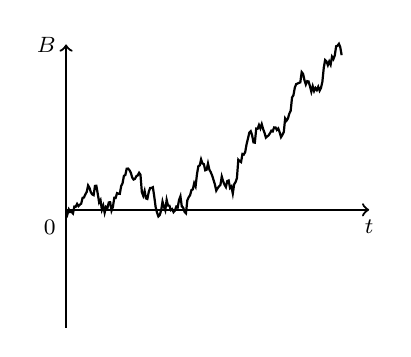
\begin{tikzpicture}[xscale=3.5]
\draw[thick,->] (0,0) node[below left] {\footnotesize $0$} -- (1.1,0) node[below] {\footnotesize $t$};
\draw[thick,->] (0,-1.5) -- (0,2.1) node[left] {\footnotesize $B$};
\draw[thick] (0.000,0.000)--(0.005,-0.056)--(0.010,0.004)--(0.015,-0.029)--(0.020,-0.027)--(0.025,-0.046)--(0.030,0.041)--(0.035,0.039)--(0.040,0.075)--(0.045,0.047)--(0.050,0.065)--(0.055,0.079)--(0.060,0.152)--(0.065,0.157)--(0.070,0.197)--(0.075,0.227)--(0.080,0.309)--(0.085,0.279)--(0.090,0.223)--(0.095,0.196)--(0.100,0.187)--(0.105,0.304)--(0.110,0.305)--(0.115,0.203)--(0.120,0.094)--(0.125,0.124)--(0.130,0.002)--(0.135,0.053)--(0.140,-0.036)--(0.145,0.036)--(0.150,0.019)--(0.155,0.094)--(0.160,0.096)--(0.165,-0.010)--(0.170,0.038)--(0.175,0.153)--(0.180,0.151)--(0.185,0.212)--(0.190,0.205)--(0.195,0.203)--(0.200,0.301)--(0.205,0.338)--(0.210,0.432)--(0.215,0.441)--(0.220,0.522)--(0.225,0.524)--(0.230,0.504)--(0.235,0.471)--(0.240,0.411)--(0.245,0.385)--(0.250,0.394)--(0.255,0.427)--(0.260,0.436)--(0.265,0.470)--(0.270,0.445)--(0.275,0.226)--(0.280,0.179)--(0.285,0.240)--(0.290,0.145)--(0.295,0.138)--(0.300,0.227)--(0.305,0.277)--(0.310,0.278)--(0.315,0.287)--(0.320,0.169)--(0.325,0.035)--(0.330,-0.034)--(0.335,-0.084)--(0.340,-0.065)--(0.345,-0.007)--(0.350,0.104)--(0.355,0.038)--(0.360,-0.007)--(0.365,0.126)--(0.370,0.054)--(0.375,0.053)--(0.380,-0.003)--(0.385,0.009)--(0.390,-0.029)--(0.395,-0.009)--(0.400,0.040)--(0.405,0.029)--(0.410,0.125)--(0.415,0.172)--(0.420,0.043)--(0.425,0.028)--(0.430,-0.027)--(0.435,-0.044)--(0.440,0.120)--(0.445,0.160)--(0.450,0.185)--(0.455,0.251)--(0.460,0.260)--(0.465,0.339)--(0.470,0.299)--(0.475,0.451)--(0.480,0.554)--(0.485,0.564)--(0.490,0.641)--(0.495,0.589)--(0.500,0.580)--(0.505,0.502)--(0.510,0.509)--(0.515,0.588)--(0.520,0.510)--(0.525,0.478)--(0.530,0.436)--(0.535,0.381)--(0.540,0.323)--(0.545,0.244)--(0.550,0.275)--(0.555,0.298)--(0.560,0.316)--(0.565,0.422)--(0.570,0.362)--(0.575,0.319)--(0.580,0.289)--(0.585,0.365)--(0.590,0.372)--(0.595,0.278)--(0.600,0.298)--(0.605,0.208)--(0.610,0.324)--(0.615,0.352)--(0.620,0.402)--(0.625,0.636)--(0.630,0.617)--(0.635,0.606)--(0.640,0.709)--(0.645,0.702)--(0.650,0.734)--(0.655,0.832)--(0.660,0.905)--(0.665,0.981)--(0.670,0.999)--(0.675,0.949)--(0.680,0.857)--(0.685,0.853)--(0.690,1.031)--(0.695,1.029)--(0.700,1.077)--(0.705,1.034)--(0.710,1.088)--(0.715,1.026)--(0.720,0.980)--(0.725,0.917)--(0.730,0.932)--(0.735,0.946)--(0.740,0.973)--(0.745,1.005)--(0.750,0.996)--(0.755,1.047)--(0.760,1.046)--(0.765,1.014)--(0.770,1.033)--(0.775,0.986)--(0.780,0.923)--(0.785,0.951)--(0.790,0.987)--(0.795,1.160)--(0.800,1.133)--(0.805,1.159)--(0.810,1.221)--(0.815,1.257)--(0.820,1.427)--(0.825,1.454)--(0.830,1.552)--(0.835,1.596)--(0.840,1.604)--(0.845,1.612)--(0.850,1.619)--(0.855,1.749)--(0.860,1.727)--(0.865,1.647)--(0.870,1.592)--(0.875,1.634)--(0.880,1.630)--(0.885,1.570)--(0.890,1.500)--(0.895,1.569)--(0.900,1.509)--(0.905,1.547)--(0.910,1.521)--(0.915,1.562)--(0.920,1.513)--(0.925,1.549)--(0.930,1.625)--(0.935,1.801)--(0.940,1.902)--(0.945,1.885)--(0.950,1.837)--(0.955,1.884)--(0.960,1.844)--(0.965,1.944)--(0.970,1.914)--(0.975,1.960)--(0.980,2.077)--(0.985,2.084)--(0.990,2.108)--(0.995,2.064)--(1.000,1.964);

\end{tikzpicture}
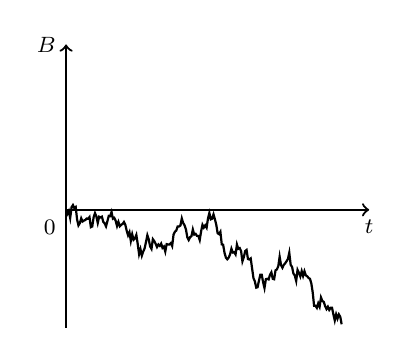
\begin{tikzpicture}[xscale=3.5]
\draw[thick,->] (0,0) node[below left] {\footnotesize $0$} -- (1.1,0) node[below] {\footnotesize $t$};
\draw[thick,->] (0,-1.5) -- (0,2.1) node[left] {\footnotesize $B$};
\draw[thick] (0.000,0.000)--(0.005,-0.051)--(0.010,-0.015)--(0.015,-0.103)--(0.020,0.033)--(0.025,0.060)--(0.030,0.022)--(0.035,0.036)--(0.040,-0.122)--(0.045,-0.198)--(0.050,-0.169)--(0.055,-0.108)--(0.060,-0.148)--(0.065,-0.136)--(0.070,-0.129)--(0.075,-0.111)--(0.080,-0.114)--(0.085,-0.092)--(0.090,-0.220)--(0.095,-0.212)--(0.100,-0.096)--(0.105,-0.042)--(0.110,-0.084)--(0.115,-0.166)--(0.120,-0.088)--(0.125,-0.097)--(0.130,-0.087)--(0.135,-0.152)--(0.140,-0.173)--(0.145,-0.210)--(0.150,-0.145)--(0.155,-0.077)--(0.160,-0.080)--(0.165,-0.028)--(0.170,-0.112)--(0.175,-0.102)--(0.180,-0.139)--(0.185,-0.206)--(0.190,-0.154)--(0.195,-0.209)--(0.200,-0.190)--(0.205,-0.181)--(0.210,-0.155)--(0.215,-0.189)--(0.220,-0.265)--(0.225,-0.324)--(0.230,-0.284)--(0.235,-0.395)--(0.240,-0.311)--(0.245,-0.380)--(0.250,-0.363)--(0.255,-0.319)--(0.260,-0.433)--(0.265,-0.563)--(0.270,-0.500)--(0.275,-0.582)--(0.280,-0.530)--(0.285,-0.491)--(0.290,-0.409)--(0.295,-0.323)--(0.300,-0.376)--(0.305,-0.464)--(0.310,-0.496)--(0.315,-0.373)--(0.320,-0.397)--(0.325,-0.431)--(0.330,-0.473)--(0.335,-0.440)--(0.340,-0.458)--(0.345,-0.429)--(0.350,-0.483)--(0.355,-0.466)--(0.360,-0.530)--(0.365,-0.436)--(0.370,-0.440)--(0.375,-0.440)--(0.380,-0.423)--(0.385,-0.460)--(0.390,-0.314)--(0.395,-0.278)--(0.400,-0.262)--(0.405,-0.211)--(0.410,-0.211)--(0.415,-0.199)--(0.420,-0.110)--(0.425,-0.169)--(0.430,-0.196)--(0.435,-0.249)--(0.440,-0.349)--(0.445,-0.383)--(0.450,-0.347)--(0.455,-0.335)--(0.460,-0.250)--(0.465,-0.314)--(0.470,-0.305)--(0.475,-0.331)--(0.480,-0.331)--(0.485,-0.383)--(0.490,-0.275)--(0.495,-0.190)--(0.500,-0.225)--(0.505,-0.197)--(0.510,-0.227)--(0.515,-0.110)--(0.520,-0.041)--(0.525,-0.121)--(0.530,-0.113)--(0.535,-0.058)--(0.540,-0.118)--(0.545,-0.188)--(0.550,-0.297)--(0.555,-0.309)--(0.560,-0.279)--(0.565,-0.439)--(0.570,-0.443)--(0.575,-0.547)--(0.580,-0.607)--(0.585,-0.628)--(0.590,-0.608)--(0.595,-0.567)--(0.600,-0.494)--(0.605,-0.542)--(0.610,-0.537)--(0.615,-0.566)--(0.620,-0.441)--(0.625,-0.495)--(0.630,-0.486)--(0.635,-0.522)--(0.640,-0.655)--(0.645,-0.602)--(0.650,-0.524)--(0.655,-0.510)--(0.660,-0.625)--(0.665,-0.631)--(0.670,-0.617)--(0.675,-0.744)--(0.680,-0.867)--(0.685,-0.908)--(0.690,-0.988)--(0.695,-0.982)--(0.700,-0.899)--(0.705,-0.823)--(0.710,-0.823)--(0.715,-0.920)--(0.720,-0.993)--(0.725,-0.881)--(0.730,-0.876)--(0.735,-0.884)--(0.740,-0.825)--(0.745,-0.794)--(0.750,-0.876)--(0.755,-0.882)--(0.760,-0.769)--(0.765,-0.757)--(0.770,-0.716)--(0.775,-0.595)--(0.780,-0.702)--(0.785,-0.736)--(0.790,-0.700)--(0.795,-0.679)--(0.800,-0.653)--(0.805,-0.625)--(0.810,-0.545)--(0.815,-0.699)--(0.820,-0.724)--(0.825,-0.809)--(0.830,-0.835)--(0.835,-0.903)--(0.840,-0.763)--(0.845,-0.799)--(0.850,-0.846)--(0.855,-0.779)--(0.860,-0.840)--(0.865,-0.780)--(0.870,-0.832)--(0.875,-0.844)--(0.880,-0.866)--(0.885,-0.876)--(0.890,-0.935)--(0.895,-1.049)--(0.900,-1.219)--(0.905,-1.219)--(0.910,-1.245)--(0.915,-1.188)--(0.920,-1.231)--(0.925,-1.114)--(0.930,-1.157)--(0.935,-1.169)--(0.940,-1.223)--(0.945,-1.260)--(0.950,-1.231)--(0.955,-1.271)--(0.960,-1.244)--(0.965,-1.244)--(0.970,-1.327)--(0.975,-1.405)--(0.980,-1.328)--(0.985,-1.381)--(0.990,-1.329)--(0.995,-1.359)--(1.000,-1.454);

\end{tikzpicture}
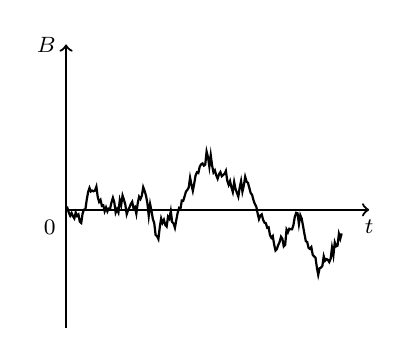
\begin{tikzpicture}[xscale=3.5]
\draw[thick,->] (0,0) node[below left] {\footnotesize $0$} -- (1.1,0) node[below] {\footnotesize $t$};
\draw[thick,->] (0,-1.5) -- (0,2.1) node[left] {\footnotesize $B$};
\draw[thick] (0.000,0.000)--(0.005,0.021)--(0.010,-0.036)--(0.015,-0.075)--(0.020,-0.041)--(0.025,-0.082)--(0.030,-0.109)--(0.035,-0.034)--(0.040,-0.078)--(0.045,-0.060)--(0.050,-0.152)--(0.055,-0.167)--(0.060,-0.047)--(0.065,0.002)--(0.070,0.002)--(0.075,0.128)--(0.080,0.225)--(0.085,0.278)--(0.090,0.233)--(0.095,0.244)--(0.100,0.235)--(0.105,0.244)--(0.110,0.294)--(0.115,0.162)--(0.120,0.101)--(0.125,0.126)--(0.130,0.051)--(0.135,0.058)--(0.140,-0.018)--(0.145,0.030)--(0.150,-0.020)--(0.155,0.018)--(0.160,0.019)--(0.165,0.095)--(0.170,0.153)--(0.175,0.097)--(0.180,-0.035)--(0.185,0.008)--(0.190,-0.033)--(0.195,0.124)--(0.200,0.061)--(0.205,0.181)--(0.210,0.127)--(0.215,0.067)--(0.220,-0.056)--(0.225,-0.005)--(0.230,0.029)--(0.235,0.074)--(0.240,0.102)--(0.245,0.014)--(0.250,0.034)--(0.255,-0.049)--(0.260,0.083)--(0.265,0.166)--(0.270,0.137)--(0.275,0.180)--(0.280,0.287)--(0.285,0.240)--(0.290,0.181)--(0.295,0.085)--(0.300,-0.076)--(0.305,0.071)--(0.310,-0.014)--(0.315,-0.117)--(0.320,-0.170)--(0.325,-0.321)--(0.330,-0.334)--(0.335,-0.371)--(0.340,-0.223)--(0.345,-0.110)--(0.350,-0.165)--(0.355,-0.127)--(0.360,-0.192)--(0.365,-0.212)--(0.370,-0.088)--(0.375,-0.114)--(0.380,-0.018)--(0.385,-0.155)--(0.390,-0.172)--(0.395,-0.228)--(0.400,-0.131)--(0.405,-0.038)--(0.410,0.022)--(0.415,0.009)--(0.420,0.118)--(0.425,0.114)--(0.430,0.169)--(0.435,0.231)--(0.440,0.252)--(0.445,0.283)--(0.450,0.408)--(0.455,0.318)--(0.460,0.241)--(0.465,0.332)--(0.470,0.437)--(0.475,0.476)--(0.480,0.467)--(0.485,0.548)--(0.490,0.577)--(0.495,0.589)--(0.500,0.561)--(0.505,0.574)--(0.510,0.740)--(0.515,0.670)--(0.520,0.549)--(0.525,0.694)--(0.530,0.561)--(0.535,0.475)--(0.540,0.501)--(0.545,0.437)--(0.550,0.395)--(0.555,0.452)--(0.560,0.479)--(0.565,0.427)--(0.570,0.443)--(0.575,0.457)--(0.580,0.494)--(0.585,0.368)--(0.590,0.317)--(0.595,0.365)--(0.600,0.287)--(0.605,0.227)--(0.610,0.352)--(0.615,0.263)--(0.620,0.216)--(0.625,0.167)--(0.630,0.282)--(0.635,0.364)--(0.640,0.231)--(0.645,0.308)--(0.650,0.419)--(0.655,0.359)--(0.660,0.343)--(0.665,0.279)--(0.670,0.212)--(0.675,0.191)--(0.680,0.124)--(0.685,0.074)--(0.690,0.043)--(0.695,-0.045)--(0.700,-0.118)--(0.705,-0.073)--(0.710,-0.058)--(0.715,-0.126)--(0.720,-0.164)--(0.725,-0.171)--(0.730,-0.229)--(0.735,-0.223)--(0.740,-0.323)--(0.745,-0.355)--(0.750,-0.333)--(0.755,-0.441)--(0.760,-0.517)--(0.765,-0.498)--(0.770,-0.446)--(0.775,-0.407)--(0.780,-0.342)--(0.785,-0.368)--(0.790,-0.464)--(0.795,-0.445)--(0.800,-0.252)--(0.805,-0.286)--(0.810,-0.240)--(0.815,-0.247)--(0.820,-0.247)--(0.825,-0.195)--(0.830,-0.089)--(0.835,-0.038)--(0.840,-0.044)--(0.845,-0.181)--(0.850,-0.069)--(0.855,-0.111)--(0.860,-0.208)--(0.865,-0.307)--(0.870,-0.397)--(0.875,-0.409)--(0.880,-0.484)--(0.885,-0.497)--(0.890,-0.474)--(0.895,-0.572)--(0.900,-0.591)--(0.905,-0.607)--(0.910,-0.731)--(0.915,-0.826)--(0.920,-0.742)--(0.925,-0.734)--(0.930,-0.713)--(0.935,-0.589)--(0.940,-0.646)--(0.945,-0.626)--(0.950,-0.634)--(0.955,-0.663)--(0.960,-0.622)--(0.965,-0.482)--(0.970,-0.579)--(0.975,-0.414)--(0.980,-0.464)--(0.985,-0.456)--(0.990,-0.307)--(0.995,-0.367)--(1.000,-0.300);

\end{tikzpicture}
\caption{Траектории броуновского движения.}
\label{6:trajectory}
\end{figure}


\subsection{Мартингальное и марковское свойства броуновского движения}

\begin{definition}
Случайный процесс $X$ называется \emph{мартингалом} относительно фильтрации $\FF$, если
\begin{alphenum}
\item он согласован с фильтрацией $\FF$;
\item $\E|X_t| < \infty$ для всех $t$;
\item $\E(X_t\mid\F_s) = X_s$ \as\ для всех $s\le t$.
\end{alphenum}
Если в последнем условии заменить равенство на неравенство $\ge$, то получим определение \emph{субмартингала}, а если на $\le$, то определение \emph{супермартингала}.
\end{definition}

\begin{proposition}
Броуновское движение является мартингалом.
\end{proposition}
\begin{proof}
Имеем
\[
\E(W_t\mid\F_s) = \E(W_t - W_s + W_s\mid\F_s) 
= W_s + \E(W_t - W_s) = W_s,
\]
где воспользовались тем, что приращение $W_t - W_s$ не зависит от $\F_s$ и имеет нулевое математическое ожидание.
\end{proof}

\begin{remark}
Точно так же доказывается, что любой процесс с независимыми приращениями и $\E X_t\equiv c$ является мартингалом.  
\end{remark}

\begin{definition}
Процесс $X$ называется \emph{марковским} относительно фильтрации $\FF$, если для любых $s\le t_1<\dots<t_n$ и борелевских множеств $A_1,\dots,A_n$ выполнено равенство%
\footnote{Условная вероятность события $B$ относительно $\sigma$-алгебры $\G$ определяется как условное математическое ожидание соответствующего индикатора: $\P(B\mid\G) = \E (I_B \mid \G)$.}
\begin{equation}
\label{5:markov}
\P(X_{t_1}\in A_1,\dots,X_{t_n}\in A_n\mid\F_s) = \P(X_{t_1}\in A_1,\dots,X_{t_n}\in A_n\mid X_s)\ \text{п.н.}
\end{equation}
\end{definition}

Смысл этого определения состоит в следующем: для того, чтобы знать условное распределение значений процесса в будущем (\te\ конечномерное распределение $(X_{t_1},\dots,X_{t_n})$), достаточно знать его значение в текущий момент времени $s$, но не нужно знать всю предыдущую информацию, содержащуюся в $\F_s$.

Эквивалентное определение марковского процесса можно получить, если заменить формулу \eqref{5:markov} на условие, что для любой функции $f$, удовлетворяющей условию $\E|f(X_{t_1},\dots,X_{t_n})|<\infty$, выполнено равенство
\[
\E(f(X_{t_1},\dots,X_{t_n})\mid\F_s) = \E(f(X_{t_1},\dots,X_{t_n})\mid X_s)\ \text{п.н.}
\]

Следующее определение дает удобное понятие для работы с условными распределениями марковского процесса.

\begin{definition}
\label{pr:markov-transition}
Функция $\P(s,x,t,A)$ с аргументами $0\le s \le t$, $x\in\R$, $A\in\B(\R)$ называется \emph{марковской переходной функцией}, если
\begin{alphenum}
\item при фиксированных $s,x,t$ функция $B\mapsto P(s,x,t,A)$ является вероятностной мерой на $\B(\R)$;
\item при фиксированных $s,t,A$ функция $x\mapsto P(s,x,t,A)$ измерима;
\item $\P(s,x,s,A) = \I(x\in A)$ для любых $s,x,A$;
\item для любого $u\in[s,t]$ выполнено \emph{уравнение Колмогорова"--~Чепмена}:
\[
P(s,x,t,A) = \int_\R P(u,y,t,A) P(s,x,u,\,dy).
\]
\end{alphenum}
Говорят, что марковский процесс $X$ обладает переходной функцией $\P(s,x,t,A)$, если $\P(X_t \in A\mid X_s = x) = \P(s,x,t,A)$ \as\ для всех $s,x,t,A$.
%\footnote{Напомним, что условное математическое ожидание $\E(X\mid Y)$ можно представить как функцию $g(Y)$.
%Тогда запись $\E(X\mid Y=y)$ обозначает значение $g(y)$; см.~лекцию \ref{ch:mart}.}
\end{definition}

Переходную функцию нужно понимать как вероятность того, что, начиная из точки $x$ в момент времени $s$, процесс попадет в множество $A$ в момент времени $t$.
Условия a) и b) в определении \ref{pr:markov-transition} "--- технические, они гарантируют, что переходная функция <<хорошо устроена>>.
Условие c) означает, что если $t=s$, то процесс <<никуда не уйдет>> за нулевое время.
Уравнение Колмогорова"--~Чепмена (условие d) имеет следующий смысл: вероятность перехода из точки $x$ в множество $A$ за время $[s,t]$ может быть найдена из вероятностей перехода из точки $x$ в промежуточную точку $y$ за время $[s,u]$ и из $y$ в множество $A$ за время $[u,t]$, где $y$ пробегает всевозможные значения.

Известно, что у любого марковского процесса со значениями в $\R$ (или в $\R^n$) переходная функция существует.

\begin{definition}
Марковская переходная функция (или соответствующий ей марковский процесс) называется \emph{однородной}, если она зависит только от разности $t-s$, \te\ $\P(s,x,t,A) = \P(0,x,t-s,A)$.
\end{definition}

\begin{definition}
Если для всех $s<t$ и $x$ переходная функция марковского процесса $X$ обладает плотностью $p(s,x,t,y)$, \te\ выполнено равенство
\[
\P(s,x,t,A) = \int_A p(s,x,t,y)\,dy,
\]
то функция $p(s,x,t,y)$ называется \emph{переходной плотностью} процесса $X$.
\end{definition}

\begin{proposition}
Броуновское движение является однородным марковским процессом с переходной плотностью
\[
p(s,x,t,y) = \frac{1}{\sqrt{2\pi(t-s)}}\exp\left(-\frac{(y-x)^2}{2(t-s)}\right).
\] 
\end{proposition}
\begin{remark}
Легко заметить, что $p(s,x,t,y)$ есть плотность нормального распределения со средним $x$ и дисперсией $t-s$.
\end{remark}
\begin{proof}
Марковское свойство следует из того, что приращения $W_{t_i}-W_s$ не зависят от $\F_s$ при $t_i>s$, и, следовательно%
\footnote{Здесь используется такой факт: если случайная величина $Y$ является $\G$-измеримой, а случайный вектор $X$ не зависит от $\G$, то $\E(f(X,Y) \mid \G) = g(Y)$, где $g(y) = \E(f(X,y))$.
Результат справедлив при условии, что $\E| f(X,Y)| < \infty$.}, 
\[
\E( f(W_{t_1}, \ldots, W_{t_n}) \mid \F_s)
= \E( f(W_{t_1} - W_s + W_s, \ldots, W_{t_n} - W_s + W_s) \mid \F_s)
= g(W_s),
\]
где $g(x) = \E f(W_{t_1} - W_s + x, \ldots, W_{t_n} - W_s + x)$.
Аналогично получаем
\[
\P(W_t \in B \mid W_s = x) = \P( W_t - W_s + x \in B),
\]
и тогда формула для переходной плотности следует из того, что $W_t - W_s$ имеет нормальное распределение с нулевым средним и дисперсией $t-s$.
\end{proof}


\section{Броуновское движение со сносом и геометрическое броуновское движение}

\begin{definition}
Броуновским движением с коэффициентом \emph{сноса} $\mu\in\R$, коэффициентом \emph{диффузии} $\sigma>0$ и начальным условием $x\in\R$ относительно фильтрации $\FF$ называется процесс
\[
X_t = x + \mu t + \sigma W_t,
\]
где $W$ "--- броуновское движение относительно $\FF$.

Иногда такой процесс называют \emph{общим броуновским движением} (или даже просто броуновским движением, а для $x=0$, $\mu=0$, $\sigma=1$ используют термин \emph{стандартное броуновское движение}).
\end{definition}

Следующий результат непосредственно вытекает из свойств стандартного броуновского движения.

\begin{proposition}
Общее броуновское движение является однородным марковским процессом.
Оно является мартингалом при $\mu=0$, субмартингалом при $\mu\ge0$ и супермартингалом при $\mu\le0$.
\end{proposition}

\begin{definition}
\emph{Геометрическим броуновским движением} с коэффициентом \emph{сноса} $\mu\in\R$, коэффициентом \emph{волатильности} $\sigma>0$ и начальным условием $s>0$ относительно фильтрации $\FF$ называется процесс
\[
S_t = s e^{\sigma W_t + (\mu-\frac{\sigma^2}{2})t},
\]
где $W$ "--- броуновское движение относительно $\FF$.
\end{definition}

Качественное отличие геометрического броуновского движения от обычного такое же как у мультипликативного случайного блуждания от аддитивного (см.~примеры в лекции~3).
В частности, у геометрического броуновского движения нормально распределены и независимы приращения его логарифма, а не самого процесса. 

Геометрическое броуновское движение будет играть важную роль в дальнейшем изложении.
В частности, оно задает цену рискового актива в модели \bs.

Отметим, что странный на первый взгляд член $-\frac{\sigma^2}{2}t$ в экспоненте вводится для того, чтобы сделать геометрическое броуновское движение мартингалом в случае $\mu=0$, как показывает следующее предложение.

\begin{proposition}
Геометрическое броуновское движение является однородным марковским процессом.
Оно является мартингалом при $\mu=0$, субмартингалом при $\mu\ge0$ и супермартингалом при $\mu\ge0$.
Кроме того, $\E S_t = s e^{\mu t}$.
\end{proposition}

\begin{proof}
Марковское свойство следует из того, что имеется взаимно"=однозначное соответствие между $S_t$ и $W_t$.
Мартингальное (или суб/супермартингальное) свойство следует из равенства
\[
\E (S_t \mid \F_u) = S_u \E(e^{(\mu-\frac{\sigma^2}{2})(t-u) + \sigma(W_t-W_u)}) = S_u e^{\mu(t-u)},
\]
где воспользовались тем, что $\E e^{\sigma (W_t-W_u)} = e^{\frac{\sigma^2}{2} (t-u)}$.
\end{proof}


\summary

\begin{itemize}
\item В этом курсе случайные процессы рассматриваются на фильтрованных вероятностных пространствах $(\Omega,\F,\FF,\P)$. Случайный процесс $
X$ называется согласованным с фильтрацией $\FF$, если для каждого $t$ случайная величина $X_t$ измерима относительно $\F_t$.

\item Определение броуновского движения: непрерывный случайный процесс с нулевым начальным значением и независимыми приращениями, которые имеют нормальное распределение со средним 0 и дисперсией $\D (W_t-W_s) = t-s$. Эквивалентное определение: непрерывный гауссовский процесс с нулевым средним и ковариационной функцией $\cov(W_t,W_s) = \min(s,t)$.

\item Броуновское движение является мартингалом и марковским процессом, у которого переходные вероятности задаются нормальным распределением.

\item Общее броуновское движение "--- это процесс $X_t = x + \mu t + \sigma W_t$.

\item Геометрическое броуновское движение "--- это процесс $S_t = s e^{\sigma W_t + (\mu-\frac{\sigma^2}{2})t}$. При $\mu=0$ он является мартингалом.
\end{itemize}

%!TEX root=finmath1.tex
\chapter{Интеграл Ито}
\label{ch:ito-integral}
\chaptertoc

В этой лекции мы определим стохастический интеграл по броуновскому движению (\emph{интеграл Ито})
\[
\int_0^t H_s d W_s,
\]
где $H$ -- случайный процесс, а $W$ -- стандартное броуновское движение.
Мы также получим \emph{формулу Ито} о дифференцировании функций от броуновского движения.
Эти теоретические понятия необходимы для построения моделей рынков с непрерывным временем.


\section{Конструкция интеграла Ито}

Трудность определения интеграла по броуновскому движению состоит в том, что его нельзя определить потраекторно, \te\ зафиксировать $\omega$ и вычислить $\int_0^t H_s(\omega) d W_s(\omega)$.
Действительно, написать $\int_0^t H_s(\omega) W_s'(\omega) ds$ нельзя, так как траектории броуновского движения не дифференцируемы.
Не получится воспользоваться и интегралами Римана"--~Стилтьеса или Лебега"--~Стилтьеса, так как броуновское движение имеет траектории неограниченной вариации. 

Конструкция интеграла Ито будет дана в три этапа.
Сначала мы определим его для кусочно-постоянных случайных процессов $H$ (называемых \emph{простыми}).
Затем распространим определение интеграла на согласованные измеримые процессы $H$, удовлетворяющие условию $\E \int_0^t H_s^2 ds <\infty$.
Наконец, общая конструкция интеграла будет дана для согласованных измеримых процессов со свойством $\int_0^t H_s^2 ds < \infty$ \as


\subsection{Интеграл Ито для простых процессов}

Пусть задано фильтрованное вероятностное пространство $(\Omega, \F, \FF, \P)$ и стандартное броуновское движение $W$ на нем.
Для начала будем считать временной горизонт ограниченным моментом времени $T$, поэтому все процессы будут рассматриваться на отрезке $[0,T]$.

\begin{definition}
Случайный процесс $H=(H_t)_{t\in[0,T]}$ называется \emph{простым}, если его можно представить в виде
\begin{equation}
\label{7:simple}
H_t = \xi_0 \I(t=0) + \sum_{i=1}^n \xi_i \I(t \in (t_{i-1}, t_i]),
\end{equation}
где $0= t_0 < \ldots < t_n =  T$, а $\xi_i$ являются $\F_{t_{i-1}}$-измеримыми ограниченными%
\footnote{Ограниченность означает, что $|\xi_i| \le c$ \as\ для некоторой константы $c$.}
случайными величинами.
\end{definition}

Таким образом, у простого процесса траектории кусочно постоянны, а на каждом интервале постоянства $(t_{i-1},t_i]$ значение траектории является случайной величиной, измеримой относительно $\F_{t_{i-1}}$.

\begin{definition}
Для простого процесса $H$ определим \emph{интеграл Ито} на отрезке $[0,T]$ как случайную величину
\begin{equation}
\int_0^T H_s d W_s 
= \sum_{i=1}^n \xi_i (W_{t_i} - W_{t_{i-1}}).
\end{equation}
\end{definition}

Идея этого определения довольно естественна: так как процесс $H$ кусочно постоянный, то в качестве значения интеграла нужно взять сумму значений этого процесса на каждом отрезке постоянства, умноженную на приращение броуновского движения.
Заметим, что значение $H_0$ (\te\ $\xi_0$) не учитывается. 

Необходимо показать корректность определения: если представить простой процесс $H$ по формуле \eqref{7:simple} двумя способами с разными разбиениями, то значения интегралов совпадут.
Это можно сделать с помощью перехода к объединенному разбиению.
Доказательство остается в качестве упражнения.

\begin{definition}
Для простого процесса $H$ определим интеграл Ито с переменным верхним пределом $t\in[0,T]$ как случайный процесс $\int_0^t H_s d W_s = I_t(H)$, где
\begin{equation}
I_t(H) = \int_0^T H_s \I(s\le t) d W_s
\end{equation}
(интеграл в правой части определен, так как  $H_s\I(s\le t)$ "--- простой процесс).

В явном виде имеем
\begin{equation}
\label{7:simple-integral}
\begin{aligned}
\int_0^t H_s d W_s &= \sum_{i=1}^n \xi_i (W_{t\wedge t_i} - W_{t\wedge t_{i-1}}) \\
& = \sum_{i=1}^k \xi_i (W_{t_i} - W_{t_{i-1}}) + \xi_{k+1} (W_t - W_{t_k})\ \text{для}\ t\in(t_k,t_{k+1}].
\end{aligned}
\end{equation}
\end{definition}

Далее, говоря <<интеграл Ито>>, мы, как правило, будем иметь ввиду именно интеграл с переменным верхним пределом, и для нас будут важны свойства, которыми он обладает как случайный процесс: (непрерывность траекторий, мартингальное свойство и \td).

\begin{proposition}
Пусть $H$ "--- простой процесс.
Тогда процесс $I_t(H) = \int_0^t H_s dW_s$ обладает следующими свойствами:
\begin{alphenum}
\item $I_t(H)$ является согласованным с фильтрацией $\FF$, имеет непрерывные траектории, и $I_0(H) = 0$;
\item $I_t(H)$ является мартингалом относительно $\FF$;
\item $\E I_t(H) = 0$;
\item если $G$ "--- тоже простой процесс, то $\E(I_t(H)I_t(G)) = \E \int_0^t H_sG_s ds$ и, в частности, $\E(I_t(H)^2) = \E \int_0^t H_s^2 ds$.
\end{alphenum}
\end{proposition}

\begin{remark}
В последнем свойстве можно поменять местами интеграл по $ds$ и математическое ожидание%
\footnote{Для этого можно воспользоваться теоремой Фубини, но конкретно здесь все проще, так как интеграл является конечной суммой (подынтегральное выражение кусочно-постоянно).}:
$\E(I_t(H)I_t(G)) = \int_0^t \E(H_sG_s) ds$.  
\end{remark}

\begin{proof}
Свойство а) следует из формулы \eqref{7:simple-integral} и непрерывности траекторий броуновского движения.
Конечность ожидания $\E I_t(H)$ следует опять же из этой формулы, учитывая, что величины $\xi_i$ ограничены.

Проверим мартингальное свойство $\E(I_t(H) \mid \F_s) = I_s(H)$.
Пусть $t\in (t_k,t_{k+1}]$, а $s\in (t_j, t_{j+1}]$, где $j\le k$.
Тогда из \eqref{7:simple-integral} имеем
\[
I_t(H) - I_s(H) = \xi_{j+1}(W_{t_{j+1}} - W_s) + \sum_{i=j+2}^k \xi_i(W_{t_{i+1}} - W_{t_i}) + \xi_{k+1}(W_t - W_{t_k}). 
\]
Пользуясь независимостью приращений броуновского движения, нетрудно показать, что условное ожидание $\E(\,\cdot\,|\, \F_s)$ каждого слагаемого в правой части равно нулю, и, таким образом, $\E(I_t(H) -I_s(H) \mid \F_s) = 0$.
Следовательно, $I_t(H)$ -- мартингал.
Это доказывает свойство b).
Свойство c) следует из того, что $\E I_t(H) = \E I_0(H) = 0$ в силу мартингальности.

Докажем d).
Достаточно рассмотреть случай $t=T$ (иначе возьмем процессы $\tilde H_s = H_s \I(s\le t)$ и $\tilde G_s = G_s \I(s\le t)$).
Также можно считать, что разбиения $t_i$ у процессов $H$ и $G$ совпадают (всегда можно взять общее разбиение).
Пусть
\[
H_t = \xi_0 \I(t=0) + \sum_{i=1}^n \xi_i \I(t \in (t_{i-1}, t_i]), \qquad
G_t = \eta_0 \I(t=0) + \sum_{i=1}^n \eta_i \I(t \in (t_{i-1}, t_i]).
\]
Имеем
\begin{multline*}
\E(I_T(H)I_T(G)) 
= \E\biggl(\sum_{i=1}^n \xi_i (W_{t_i} - W_{t_{i-1}}) \cdot
  \sum_{i=1}^n \eta_i (W_{t_i} - W_{t_{i-1}})\biggr) \\
= \sum_{i=1}^n \E(\xi_i\eta_i (W_{t_i} - W_{t_{i-1}})^2)
+ \sum_{i\neq j} \E(\xi_i\eta_j (W_{t_i} - W_{t_{i-1}})(W_{t_j} - W_{t_{j-1}})).
\end{multline*}
Для слагаемых в первой сумме, пользуясь независимостью приращений броуновского движения, находим
\begin{multline*}
\E(\xi_i\eta_i \E(W_{t_i} - W_{t_{i-1}})^2)
= \E(\E(\xi_i\eta_i (W_{t_i} - W_{t_{i-1}})^2 \mid \F_{t_{i-1}})) \\
= \E(\xi_i\eta_i \E(W_{t_i} - W_{t_{i-1}})^2) = \E(\xi_i\eta_i) (t_i - t_{i-1}).
\end{multline*}
Покажем, что все слагаемые во второй сумме равны нулю. Пусть $i<j$ (случай $i>j$ рассматривается аналогично). Тогда
\begin{multline*}
\E (\xi_i\eta_j (W_{t_i} - W_{t_{i-1}})(W_{t_j} - W_{t_{j-1}})) \\
= \E (\E(\xi_i\eta_j (W_{t_i} - W_{t_{i-1}}) (W_{t_j} - W_{t_{j-1}}) 
  \mid \F_{t_{j-1}}))\\
= \E (\xi_i\eta_j (W_{t_i} - W_{t_{i-1}}) \E(W_{t_j} - W_{t_{j-1}} 
  \mid \F_{t_{j-1}})) 
= 0.
\end{multline*}
В итоге получаем
\[
\E(I_T(H)I_T(G))^2 = \sum_{i=1}^n\E( \xi_i\eta_i) (t_i -t_{i-1}) =
\E\left( \sum_{i=1}^n \xi_i\eta_j (t_i -t_{i-1})\right) 
= \E \int_0^T H_sG_s ds,
\]
что и требовалось доказать.
\end{proof}


\subsection{Интеграл Ито для процессов из пространства $\L^2$}

Определенный выше интеграл Ито можно рассматривать как отображение из класса простых процессов в класс непрерывных квадратично интегрируемых мартингалов.
Каждому простому процессу оно ставит в соответствие его процесс-интеграл $I_t(H)$.
Следующий этап конструкции состоит в том, чтобы продолжить по непрерывности это отображение на более широкий класс подынтегральных процессов.
Под продолжением по непрерывности понимается то, что если простые процессы $H^n$ сходятся в подходящем смысле к процессу $H$, то нужно положить по определению $I_t(H) = \lim_{n\to\infty} I_t(H^n)$.

Чтобы говорить сходимости и непрерывности, зададим структуру метрического пространства для подынтегральных процессов и процессов-интегралов. 
Напомним, что если $(S,\mathcal{S})$ "--- измеримое пространство, а $\mu$ "--- мера на нем (конечная, но не обязательно вероятностная), то пространством $L^2(S,\mathcal{S},\mu)$ называется линейное пространство классов эквивалентности измеримых функций $f(s)$ на $(S,\mathcal{S})$ таких, что $\int_S f(s)^2 \mu(ds) < \infty$.
Функции считаются эквивалентными, если они совпадают почти всюду по мере $\mu$.
Далее, как это обычно делается, мы будем опускать слова <<класс эквивалентности>>, а также писать просто $L^2$, когда ясно о каком измеримом пространстве и мере идет речь.

На пространстве $L^2$ определено скалярное произведение
\[
\langle f,\, g\rangle_{L^2} = \int_S f(s)g(s) \mu(ds).
\]
Скалярное произведение порождает норму и метрику
\[
\|f\|_{L^2} = \sqrt{\langle f,\, f\rangle_{L^2}}, \qquad \rho_{L^2}(f, g) = \|f-g\|_{L^2}.
\]
Известно, что пространство $L^2$ является \emph{гильбертовым пространством}, т.е.\ линейным пространством со скалярным произведением, полным относительно порождаемой им метрики%
\footnote{Полнота означает, что любая последовательность Коши $f_n$ в $L^2$ сходится по норме к некоторой функции $f$ в $L^2$.
Последовательность $f_n$ называется \emph{последовательностью Коши}, если для любого $\epsilon>0$ найдется $N$ такое, что $\rho(f_n, f_m) < \epsilon$ для всех $n,m>N$.}.

Далее в качестве пространства $(S,\mathcal{S},\mu)$ будем рассматривать $S=\Omega\times [0,T]$, $\mathcal{S} = \F\otimes\B([0,T])$ и $\mu=\P\otimes\mathrm{Leb}$, где $\mathrm{Leb}$ "--- мера Лебега.
Измеримыми функциями на нем являются измеримые случайные процессы $H=(H_t)_{t\in[0,T]}$.

\begin{definition}
Подпространство $\L^2_T\subset L^2(\Omega\times[0,T],\ \F\otimes\B([0,T])б\ \P\otimes\mathrm{Leb})$ состоит из измеримых согласованных случайных процессов $H$.
\end{definition}

Нетрудно заметить, что все простые процессы лежат в $\L^2_T$.
Следующее предложение устанавливает ключевое свойство, нужное для продолжения интеграла Ито с простых процессов на всё $\L^2_T$.

\begin{proposition}
Множество простых процессов всюду плотно%
\footnote{Для любого $H\in\L^2_T$ и $\epsilon>0$ найдется простой процесс $H'$ такой, что $\|H-H'\|_{L^2} \le \epsilon$.}
в $\L^2_T$.
\end{proposition}

Доказательство этого результата довольно трудное.
В полном виде его можно найти в книге \cite{LiptserShiryaev74}, глава 4, лемма 4.4. 


\medskip
Зададим теперь подходящее гильбертово пространство, в котором будут лежать процессы-интегралы.

\begin{definition}
Линейное пространство $\M^{2,c,0}_T$ \emph{непрерывных квадратично интегрируемых мартингалов с нулевым начальным значением} состоит из непрерывных мартингалов $M=(M_t)_{t\in[0,T]}$ c $M_0=0$ и $\E M_T^2 < \infty$.

Будем считать процессы $M,N\in \M_T^{2,c,0}$ эквивалентными, если они неразличимы.
На пространстве классов эквивалентности таких процессов определим скалярное произведение
\[
\langle M,N\rangle_{\M^2} = \E M_TN_T
\]
и будем обозначать за $\|M\|_{\M^2} = \sqrt{\langle M,M\rangle_{\M^2}}$ и $\rho_{\M^2}(M,N) = \|M-N\|_{\M^2}$ соответствующую норму и метрику.
\end{definition}

\begin{remark}
Если $M,N\in \M_T^{2,c,0}$, то они неразличимы тогда и только тогда, когда $M_T=N_T$ \as\ 
Действительно, если $M_T = N_T$ \as, то из мартингального свойства получаем, что $M_t = N_t$ \as\ для любого $t\le T$, \te\ $M$ является модификацией $N$.
В силу непрерывности процессов отсюда следует неразличимость.
Обратное утверждение очевидно.
\end{remark}

\begin{proposition}[см.~\cite{BulinskiShiryaev04}, глава VIII, лемма 2]
Пространство $M_T^{2,c,0}$ является гильбертовым.
\end{proposition}

Наконец, докажем лемму общего характера, из которой будет следовать возможность продолжения интеграла Ито.

\begin{lemma}[об изометрии]
Пусть $L,M$ "--- два метрических пространства, причем пространство $M$ полно.
Предположим, что на всюду плотном множестве $L_0\subset L$ задана функция $f_0\colon L_0\to M$, являющаяся изометрией, \te\ сохраняющей расстояния ($\rho_M(f(x),f(x')) = \rho_L(x,x')$ для всех $x,x'\in L_0$). 

Тогда существует единственная непрерывная функция $f\colon L\to M$ такая, что $f(x) = f_0(x)$ для всех $x\in L_0$, причем $f$ является изометрией на всем $L$.
\end{lemma}

\begin{proof}
Пусть $x\in L$.
В силу плотности $L_0$ найдется последовательность $x_n\in L_0$ такая, что $x_n\to x$.
В частности, $x_n$ является последовательностью Коши в $L$.
Тогда $f(x_n)$ является последовательностью Коши в $M$ по свойству изометрии.
Так как $M$ полно, то эта последовательность сходится к некоторому элементу $y\in M$.
Определим $f(x) = y$.

Нетрудно показать, что значение $f(x)$ не зависит от приближающей последовательности $x_n$ (если $x_n\to x$ и $x_n'\to x$, то, чтобы показать, что $y=y'$, нужно рассмотреть последовательность $x_1,x_1',x_2,x_2',\ldots$).

Функция $f$ является изометрией, так как для любых $x,x'\in L$ можно взять последовательности $x_n,x_n'\in L_0$ такие, что $x_n\to x$ и $x_n'\to x'$, и тогда
\[
\rho_M(f(x), f(x')) = \lim\limits_{n\to\infty} \rho_M(f(x_n),f(x_n')) = \lim\limits_{n\to\infty} \rho_L(x_n, x_n')_L= \rho_L(x,x'),
\]
где воспользовались непрерывностью метрики.
Из изометричности следует непрерывность, так как если $x_n\to x$ в $L$, то $\rho_M(f(x_n), f(x)) = \rho_L(x_n,x) \to 0$.

Единственность функции $f$ вытекает из ее непрерывности и плотности множества $L_0$.
\end{proof}

Теперь у нас все готово для продолжения интеграла Ито. 
Воспользуемся тем, что интеграл, заданный на множестве простых процессов, является изометрией, отображающей простые процессы в непрерывные квадратично интегрируемые мартингалы.
Следовательно, его можно единственным образом продолжить до непрерывного отображения $H\mapsto I(H)$, где $H\in \L^2_T$ и $I(H)\in \M_T^{2,c,0}$.

\begin{definition}
\emph{Интегралом Ито} процесса $H\in \L^2_T$ называется непрерывный квадратично интегрируемый мартингал $I_t(H) = \int_0^t H_s d W_s$, являющийся значением продолжения отображения $H\mapsto I(H)$ с множества простых процессов на всё $\L^2_T$.
\end{definition}

\begin{proposition}
\label{3:p:integral-properties}
Пусть $H,G\in \L^2_T$. Тогда выполнены следующие свойства.
\begin{alphenum}
\item $\int_0^t H_s d W_s = \int_0^T H_s I(s\le t) d W_s$.

\item Если случайная величина $\xi$ является $\F_u$-измеримой, $0\le u \le t$, и $\E\xi^2 < \infty$, то $\int_u^t \xi H_s dW_s = \xi \int_u^t H_s d W_s$ (где для процесса $V\in \L^2_T$ мы определяем $\int_u^t V_s dW_s = \int_0^t V_s\I(s\ge u) dW_s$).

\item $\int_0^t(aH_s+bG_s) d W_s = a\int_0^t H_s d W_s + b\int_0^t G_s d W_s$ для любых $a,b\in\R$.

\item $\E \int_0^t H_s d W_s = 0$.

\item $\E(\int_0^t H_s d W_s \cdot \int_0^t G_s d W_s) = \E \int_0^t H_sG_s ds$ (изометрия Ито).
\end{alphenum}
\end{proposition}

\begin{proof}
a) Возьмем простые процессы $H^n\to H$.
Для них непосредственно проверяется, что $\int_0^t H_s^n d W_s = \int_0^T H_s^n \I(s\le t)d W_s$.
Заметим, что процессы $H_s^n \I(s\le t)$ сходятся к $H_s\I(s\le t)$ в $\L^2_T$.
Следовательно, 
\[
\lim\limits_{n\to\infty} \int_0^T H_s^n \I(s\le t)d W_s = \int_0^T H_s\I(s\le t) dW_s.
\]
Остается показать, что $\lim\limits_{n\to\infty} \int_0^t H_s^n d W_s = \int_0^t H_s d W_s$. 
В силу мартингального свойства имеем
\[
\int_0^t H_s dW_s = \E\left(I_T(H) \mid \F_t \right), \qquad
\int_0^t H_s^n dW_s = \E\left(I_T(H^n) \mid \F_t \right).
\]
Так как случайные величины $I_T(H^n)$ сходятся к $I_T(H)$ в $L^2(\Omega,\F_T,\P)$, то сходятся и их условные ожидания.
Это доказывает свойство a).

Свойство b) доказывается аналогично.
Свойство c) для простых процессов проверяется непосредственно, а в общем случае нужно найти $H^n\to H$ и $G^n\to G$ в $\L^2$ (и тогда $aH^n+bG^n \to aH+bG)$, и перейти к пределу в соотношении $I(aH^n+bG^n) = aI(H^n) + bI(G^n)$.

Свойство d) следует из того, что $I_t(H)$ является мартингалом с нулевым начальным значением и, следовательно, нулевым средним. 

Свойство e) для $t=T$ следует из изометричности интеграла: нам нужно показать, что $\langle I_T(H), I_T(G) \rangle_{\M^2} = \langle H, G \rangle_{L^2}$, а это верно, так как изометрия сохраняет скалярные произведения%
\footnote{Если $f$ -- изометрия одного пространства со скалярным произведением в другое, то сохраняются нормы, так как $\|x\| = \rho(x,0)$.
Отсюда следует сохранение скалярных произведений, так как $\langle x,y\rangle = \frac{1}{4}(\|x+y\|^2 - \|x-y\|^2)$.}.
Чтобы получить утверждение для произвольного $t$, воспользуемся свойством a).
\end{proof}

Для полноты изложения, приведем утверждение, показывающее, как построить интеграл Ито на всей прямой.
Будем считать, что фильтрация и броуновское движение $W$ определены для всех $t\ge 0$.
Символом $\L^2_\infty$ будем обозначать линейное пространство\footnote{Пространство $\L^2_\infty$ не является гильбертовым "--- для этого нужно было бы потребовать, чтобы $\E \int_0^\infty H_s^2 ds < \infty$.} согласованных измеримых процессов $H=(H_t)_{t\ge 0}$ таких, что $\E \int_0^t H_s^2 ds < \infty$ для всех $t\ge0$.
Заметим, что $\L^2_\infty = \bigcap\limits_{T\ge0} \L^2_T$.

\begin{proposition}
Пусть $H\in\L^2_\infty$.
Тогда существует единственный непрерывный процесс $I(H) = (I_t(H))_{t\ge 0}$ такой, что $I_T(H) = \int_0^T H_t d W_t$ \as\ для всех $T\ge 0$, где интеграл понимается в смысле определения для процесса из $\L^2_T$.

Процесс $I(H)$ является мартингалом, причем $\E I_T^2(H) < \infty$ и для любого конечного момента времени $T$ он удовлетворяет всем свойствам из предыдущего предложения.
\end{proposition}

Доказательство нетрудное и основано на идее, что нужно положить по определению $I_T(H) = \sum\limits_{u=0}^\infty \int_0^T H_s d W_s \I(T \in [u, u+1))$.
Мы его здесь не приводим; детали можно найти в книге \cite{BulinskiShiryaev04}, глава VIII, теорема 2.


\subsection{\difficult\ Интеграл Ито для процессов из пространства \texorpdfstring{$\mathcal{P}^2$}{P2}}

\begin{definition}
Линейное пространство $\mathcal{P}^2_T$ состоит из согласованных измеримых случайных процессов $H=(H_t)_{t\in[0,T]}$ таких, что $\int_0^T H_t^2 dt < \infty$ \as
\end{definition}

Ясно, что $\L^2_T \subset \mathcal{P}^2_T$.
Кроме того, любой измеримый согласованный процесс, у которого траектории являются ограниченными функциями, лежит в $\mathcal{P}^2_T$.
В частности, в $\mathcal{P}^2_T$ лежат все непрерывные согласованные процессы.

Интеграл Ито может быть распространен на процессы из $\mathcal{P}^2_T$ (хотя в большинстве дальнейших применений в этом курсе достаточно будет интеграла по процессам из $\L^2_T$).
Идея состоит в том, чтобы аппроксимировать такие процессы с помощью процессов из $\L^2_T$, как показывает следующее предложение.

Дальнейшие результаты приводятся без доказательств, их можно найти в главе~4 книги \cite{LiptserShiryaev74}.


\begin{lemma}
Для любого процесса $H\in \mathcal{P}^2_T$ существует последовательность процессов $H^n \in \L^2_T$ такая, что $\int_0^T (H_s^n - H_s)^2 ds \to 0$ по вероятности при $n\to\infty$.
\end{lemma}

\begin{theorem}
Для любого процесса $H\in \mathcal{P}^2_T$ существует единственный согласованный непрерывный процесс $I_t(H)$, $t\in[0,T]$, такой, что для любой последовательности $H^n\in \L^2_T$, сходящейся к $H$ в смысле предыдущей леммы, имеем $I_t(H^n) \to I_t(H)$ по вероятности при $n\to\infty$ для всех $t\in[0,T]$.
\end{theorem}

\begin{definition}
Так определенный процесс $I_t(H)$ называется \emph{интегралом Ито} процесса $H$ и обозначается тоже как $\int_0^t H_s d W_s$.
\end{definition}

Далее аналогично рассуждениям в предыдущем разделе можно построить интеграл от процессов $H$, определенных на всех полупрямой $t\in\R_+$ и принадлежащих пространству $\mathcal{P}^2_\infty$, состоящем из измеримых согласованных процессов $H$ таких, что $\int_0^t H_t^2 dt < \infty$ \as\ для всех $t\in\R_+$.

\begin{proposition}
Интеграл Ито для процесса $H\in \mathcal{P}^2_T$ (или $H\in\mathcal{P}^2_\infty$) удовлетворяет свойствам a--c предложения \ref{3:p:integral-properties}, но в общем случае нельзя сказать, что он удовлетворяет свойствам d--e или является мартингалом.
\end{proposition}

Несмотря на то, что интеграл Ито $\int_0^t H_s d W_s$ для процесса $H\in \mathcal{P}^2_T$ не обязательно является мартингалом, он является \emph{локальным мартингалом}.
Дадим соответствующие определения.

\begin{definition}
\emph{Моментом остановки} по отношению к фильтрации $\FF$ называется неотрицательная случайная величина $\tau$ такая, что 
\[
\{\omega: \tau(\omega) \le t \} \in \F_t\ \text{для любого }\ t\ge 0.
\]
\end{definition}
Это определение аналогично определению момента остановки в случае дискретного времени (см.~лекцию \ref{ch:american-discrete}).

\begin{definition}
Если $X$ "--- случайный процесс, а $\tau$ "--- момент остановки, то процесс $X^{\tau} = (X_{t\wedge \tau})_{t\ge 0}$ называется \emph{остановленным процессом} (здесь обозначается $t\wedge \tau = \min(t,\tau)$). 
\end{definition}

\begin{definition}
Согласованный случайный процесс $X = (X_t)_{t\ge0}$ с $\E|X_0|<\infty$ называется \emph{локальным мартингалом} относительно фильтрации $\FF$, если существует последовательность моментов остановки $\tau_n$, называемая \emph{локализующей последовательностью}, такая, что
\begin{alphenum}
\item $\tau_{n+1}\ge \tau_n$ \as\ для всех $n$,
\item $\lim\limits_{n\to\infty} \tau_n = \infty$ \as,
\item $X^{\tau_n}$ является мартингалом относительно $\FF$ для каждого $n$.
\end{alphenum}
Если у процесса $X=(X_t)_{t\in[0,T]}$ горизонт времени конечен, то в свойстве 2 достаточно требовать, чтобы для почти каждого  $\omega$ нашелся номер $N$ такой, что $\tau_n(\omega) = T$ для всех $n\ge N$.
\end{definition}

\begin{remark}
Любой мартингал является локальным мартингалом.
\end{remark}

\begin{proposition}
Если $H \in \mathcal{P}^2_T$ (или $H \in \mathcal{P}^2_\infty$), то процесс $\int_0^t H_s dW_s$ является локальным мартингалом.
\end{proposition}

Следующий результат будет использован в одной из дальнейших лекций.

\begin{proposition}
Если процесс $X$ является локальным мартингалом и $X_t\ge c$ для всех $t\in[0,T]$ (или для всех $t\ge 0$), где $c$ "--- константа, то $X$ является супермартингалом.
\end{proposition}

\begin{proof}
Пусть $\tau_n$ "--- локализующая последовательность.
Тогда по мартингальному свойству остановленного процесса имеем $\E (X_{\tau_n\wedge t} \mid \F_s) = X_{\tau_n\wedge s}$ для $t\ge s$.
Перейдем к пределу $n\to\infty$. Так как $\tau_n\to\infty$, то $X_{\tau_n\wedge s} \to X_s$ и $X_{\tau_n\wedge t} \to X_t$ \as\ 
Пользуясь условной леммой Фату%
\footnote{Если $\xi^n\ge \zeta$, где $\E\zeta^- < \infty$, то $\E (\liminf\limits_{n\to\infty} \xi_n \mid \G) \le \liminf\limits_{n\to\infty} \E(\xi_n \mid \G)$.},
получаем
\[
\E (X_t \mid \F_s) = \E(\lim\limits_{n\to\infty} X_{\tau_n\wedge t} \mid \F_s) \le \liminf_{n\to\infty} \E(X_{\tau_n\wedge t} \mid \F_s) = \liminf_{n\to\infty} X_{\tau_n\wedge s} = X_s.
\]
Таким образом, выполнено супермартингальное свойство.
Взяв $s=0$ и учитывая неотрицательность $X_t$, получаем $0 \le \E X_t \le \E X_0$ и, следовательно, $\E|X_t| < \infty$.
\end{proof}


\section{Формула Ито}
\subsection{Формулировка и примеры}

\begin{theorem}[формула Ито]
Пусть функция $f(t,x)$ непрерывна и имеет непрерывные частные производные $f'_t(t,x)$, $f'_x(t,x)$ и $f''_{xx}(t,x)$. Тогда
\[
f(t, W_t) = f(0,0) + \int_0^t \left(f'_t(s,W_s) + \frac12 f''_{xx}(s,W_s)\right) ds + \int_0^t f'_x(s,W_s) dW_s,
\]
где первый интеграл понимается в смысле Римана потраекторно%
\footnote{Для каждого $\omega$ его значение равно интегралу функции $s\mapsto f'_t(s,W_s(\omega)) + \frac12 f''_{xx}(s,W_s(\omega))$.},
а второй понимается в смысле Ито.
\end{theorem}

\begin{remark}
1. Оба интеграла в формуле Ито корректно определены.
Для интеграла по $dt$ это так, потому что непрерывные функции на отрезке интегрируемы по Риману, а для интеграла по $dW_t$ под интегралом стоит согласованный непрерывный процесс, \te\ процесс из пространства $\mathcal{P}^2_\infty$.

2. Формулу Ито обычно записывают в \emph{дифференциальной форме}
\[
d f(t,W_t) = f'_t(t,W_t) dt + f'_x(t,W_t) dW_t + \frac12 f''_{xx}(t,W_t) dt.
\]
В частности, если функция $f=f(x)$ не зависит от $t$, то формула принимает вид
\[
d f(W_t) = f'(W_t) dW_t + \frac12 f''(W_t) dt.
\]
Подчеркнем, что дифференциальная форма "--- это всего лишь удобный способ записи, так как $dW_t$ не является дифференциалом в обычном смысле.
\end{remark}

\begin{example}
\label{7:e:WdW}
Пусть $f(x) = x^2$.
Подставляя в формулу Ито, получаем
\[
d W_t^2 = 2 W_t d W_t + dt.
\]
Переписывая это соотношение в интегральной форме, находим интеграл от броуновского движения по броуновскому движению:
\[
\int_0^t W_s d W_s = \frac12 (W_t^2 - t).
\]

Можно заметить отличие интеграла Ито от интеграла Римана или Лебега: для любой дифференцируемой функции $w(t)$ с $w(0)=0$ имеем $\int_0^t w(s) d w(s) = \frac12 w(t)^2$, и поправка $-\frac12 t$ не появляется.
\end{example}

\begin{example}
Пусть $X$ "--- геометрическое броуновское движение, \te
\[
X_t = x_0e^{\sigma W_t + (\mu - \frac12 \sigma^2)t}, \qquad x_0>0.
\]
Применяя формулу Ито к функции $f(t,x) = x_0 e^{\sigma x + (\mu - \frac12 \sigma^2)t}$, получаем
\[
d X_t = \mu X_t dt + \sigma X_t d W_t.
\]
Здесь процесс $X_t$ входит и в левую, и в правую часть.
Таким образом, мы получили \emph{стохастическое дифференциальное уравнение}, решением которого является геометрическое броуновское движение.
Более подробно о стохастических дифференциальных уравнениях будет рассказано в следующей лекции.
\end{example}


\subsection{\difficult\ Доказательство}

Приведем доказательство формулы Ито только для дважды непрерывно дифференцируемых функций $f(x)$, у которых производная $f'(x)$ ограничена на всей прямой.
Полное доказательство можно найти в главе~4 книги \cite{LiptserShiryaev74}.

\begin{lemma}
\label{7:l:p-convergence}
Пусть $H\in \L^2_t$ является непрерывным процессом.
Рассмотрим разбиение $t_i^n = i\frac tn$, $i=0,\dots,n$. 
Тогда
\[
\sum_{i=0}^{n-1} H_{t_i^n}(W_{t_{i+1}^n}-W_{t_i^n})^2 \xrightarrow[n\to\infty]{\P} \int_0^t H_s ds.
\]
\end{lemma}

\begin{proof}
Введем последовательности случайных величин 
\[
Z^n = \sum_{i=0}^{n-1} H_{t_i^n}(W_{t_{i+1}^n}-W_{t_i^n})^2,\qquad
Y^n = \sum_{i=0}^{n-1} H_{t_i^n}(t_{i+1}^n- t_i^n).
\]
Заметим, что, как следует из конструкции интеграла Римана,
\[
Y^n \xrightarrow[n\to\infty]{\text{п.н.}} \int_0^t H_s ds.
\]
Поэтому достаточно будет показать, что $Z^n-Y^n \xrightarrow{\P} 0$.
Имеем
\[
Z^n-Y^n = \sum_{i=0}^{n-1} H_{t_i^n}((W_{t_{i+1}^n} - W_{t_i^n})^2 - (t_{i+1}^n - t_i^n)).
\]
Из примера~\ref{7:e:WdW} следует, что $(W_s-W_r)^2 - (s-r) = 2\int_r^s W_u dW_u - W_r(W_s-W_r)$. 
Тогда получаем
\[
Z^n - Y^n 
= 2\sum_{i=0}^{n-1} H_{t_i^n} \biggl(
  \int_{t_i^n}^{t_{i+1}^n} W_s dW_s - W_{t_i^n}(W_{t^n_{i+1}}-W_{t_i^n})
\biggr) 
= 2\int_0^t H^n_s(W_s-W^n_s) dW_s,
\]
где
\[
H^n_t = \sum_{i=0}^{n-1} H_{t_i^n} \I(t\in(t_i^n,t_{i+1}^n]), \qquad
W^n_t = \sum_{i=0}^{n-1} W_{t_i^n} \I(t\in (t_i^n,t_{i+1}^n]).
\]
Пользуясь теоремой Фубини и независимостью приращений броуновского движения, находим
\[
\E \int_0^t (H_s^n (W_s - W_s^n))^2 ds = \int_0^t \E (H_s^n)^2 \E(W_s - W_s^n))^2 ds \\
\le \frac tn \int_0^t \E (H_s^n)^2 ds \to 0.
\]
Таким образом, $H^n(W-W^n) \to 0$ в $\L^2_t$, что влечет сходимость $Z^n-Y^n \to 0$ в $L^2$ и, следовательно, по вероятности.
\end{proof}

Перейдем к доказательству формулы Ито.
Для разбиения $t_i^n = i\frac tn$ имеем (опуская индекс $n$ для краткости)
\[
f(W_t) = f(0) + \sum_{i=0}^{n-1} (f(W_{t_{i+1}}) - f(W_{t_i})).
\]
Применяя формулу Тейлора с остаточным членом в форме Лагранжа, получаем
\begin{equation}
\label{7:taylor}
f(W_t) = f(0) + \sum_{i=0}^{n-1} \biggl\{f'_x(W_{t_i})(W_{t_{i+1}} - W_{t_i})
+ \frac12 f''_{xx}(W_{\tau_i})(W_{i_{i+i}}-W_{t_i})^2 \biggr\} 
\end{equation}
для некоторых точек $\tau_i \in[t_i,t_{i+1}]$, зависящих от $\omega$.
Обозначим за $X^n$ простой процесс
\[
X^n_s = \sum_{i=0}^{n-1} f'_x(W_{t_i}) \I(s\in(t_i,t_{i+1}]).
\]
Заметим, что 
\[
\sum_{i=0}^{n-1} f'_x(W_{t_i})(W_{t_{i+1}} - W_{t_i}) = \int_0^t X_s^n d W_s.
\]
Так как $f'(x)$ непрерывна, то $X^n_s(\omega) \to f'_x(W_s(\omega))$ для всех $t$ и $\omega$. Тогда в силу предположения об ограниченности $f'(x)$ имеет место сходимость $X^n\to f'_x(W)$ в $\L^2_t$, \te\ $\E \int_0^t (X_s^n - f'_x(W_s))^2 ds \to 0$ (по теореме Лебега о мажорируемой сходимости).
Следовательно,
\[
\sum_{i=0}^{n-1} f'_x(W_{t_i})(W_{t_{i+1}} - W_{t_i}) \xrightarrow[n\to\infty]{L^2} \int_0^t f'_x(W_s) d W_s.
\]
Далее преобразуем второе слагаемое под суммой в формуле \eqref{7:taylor}.
Положим
\[
\epsilon_i = f''_{xx}(W_{\tau_{i+1}}) - f''_{xx}(W_{t_i}).
\]
Так как производные функции $f$ и траектории броуновского движения непрерывны, то для фиксированного $\omega$ функция $f'_x(W_t(\omega))$ непрерывна по $t$ и, следовательно, равномерно непрерывна по $t$ на любом отрезке.
Тогда имеем $\sup_i |\epsilon_i|\to 0$ \as\ при $n\to\infty$.
Отсюда получаем
\[
\Biggl|\sum_{i=0}^{n-1} \epsilon_i (W_{t_{i+1}} - W_{t_i})^2\Biggr|
\le \sup_i |\epsilon_i| \sum_{i=0}^{n-1} (W_{t_{i+1}} - W_{t_i})^2
\xrightarrow{\P} 0,
\]
где воспользовались тем, что $\sum_{i=0}^{n-1} (W_{t_{i+1}^n}-W_{t_i^n})^2 \to t$ по вероятности, как следует из леммы~\ref{7:l:p-convergence}.
Следовательно, опять пользуясь леммой~\ref{7:l:p-convergence}, получаем
\[
\sum_{i=0}^{n-1} f''_{xx}(W_{\tau})(W_{i_{i+i}}-W_{t_i})^2
= \sum_{i=0}^{n-1} (f''_{xx}(W_{t_i}) + \epsilon_i)(W_{i_{i+i}}-W_{t_i})^2
\xrightarrow{\P} \int_0^t f''_{xx}(W_s) ds.
\]


\summary
\begin{itemize}
\item Интеграл Ито $\int_0^t H_s d W_s$ от измеримого согласованного процесса $H$ по броуновскому движению $W$ определяется в три этапа: сначала для простых процессов $H$, затем для $H\in\L^2_T$ (что означает $\E \int_0^T H_t^2 dt < \infty$), и, наконец, для $H\in\PP^2_T$ ($\int_0^T H_t^2 dt < \infty$ \as).

\item Если $H\in \L^2_T$, то интеграл Ито является квадратично интегрируемым мартингалом с нулевым средним, причем  $\E(\int_0^t H_s dW_s \cdot \int_0^t G_s d W_s) = \E\int_0^t H_sG_s ds$ для $H,G\in\L^2_T$, где $t\le T$ (изометрия Ито).
Если $H\in\PP^2_T$, то это, в общем случае, не верно.

\item Для любой функции $f(t,x)$ с непрерывными частными производными $f'_t$ и $f''_{xx}$ справедлива формула Ито:
\[
d f(t,W_t) = f'_t(t,W_t) dt + f'_x(t,W_t) dW_t + \frac12 f''_{xx}(t,W_t) dt.
\]
\end{itemize}

%!TEX root=finmath1.tex
\chapter{Процессы Ито}
\label{ch:ito-processes}
\chaptertoc

Это завершающая лекция про общую теорию случайных процессов.
В ней мы определим процессы Ито и процессы, удовлетворяющие стохастическим дифференциальным уравнениям.
Процессами такого типа задается большинство моделей в финансовой математике.


\section{Определение процессов Ито. Формула Ито}

\subsection{Одномерный случай}

Пусть задано фильтрованное вероятностное пространство $(\Omega, \F, \FF, \P)$, на котором определено броуновское движение $W$.
Горизонт времени может быть как конечным, так бесконечным.
Далее всё излагается для бесконечного горизонта, но для конечного результаты аналогичны.

Напомним, что $\PP^2$ обозначает%
\footnote{В предыдущей лекции мы писали $\PP^2_\infty$ или $\PP^2_T$.
Далее будем опускать нижний индекс, когда он ясен из контекста.}
пространство измеримых согласованных процессов $H$ таких, что $\int_0^t H_s^2 ds < \infty$ для всех $t\ge0$.
Символом $\PP^1$ будем обозначать пространство измеримых согласованных процессов $G$ со свойством $\int_0^t |G_s| ds < \infty$ для всех $t\ge0$.
Интегралы здесь понимаются потраекторно в смысле Лебега. 

\begin{definition}
Непрерывный согласованный процесс $X=(X_t)_{t\ge0}$ называется \emph{процессом Ито} (по отношению к броуновскому движению $W$), если он представим в виде
\begin{equation}
\label{8:ito}  
X_t = x_0 + \int_0^t G_s ds + \int_0^t H_s d W_s,
\end{equation}
где $x_0\in \R$ -- начальное значение процесса, а $G=(G_t)_{t\ge0}$ и $H=(H_t)_{t\ge0}$ -- измеримые согласованные процессы из пространств $\PP^1$ и $\PP^2$, соответственно.
Интеграл по $ds$ понимается потраекторно в смысле Лебега, а интеграл по $dW_s$ -- в смысле Ито.
\end{definition}

Выражение \eqref{8:ito} обычно записывают в дифференциальной форме
\begin{equation}
\label{8:ito-diff}
dX_t = G_t dt + H_t dW_t, \qquad X_0=x_0,
\end{equation}
и называют его \emph{стохастическим дифференциалом} процесса $X$.
Как и в формуле Ито, дифференциальная форма "--- это лишь удобная запись, под которой всегда подразумевается интегральное представление \eqref{8:ito}.

\begin{definition}
Пусть $X$ является процессом Ито с представлением \eqref{8:ito}, а $V$ является измеримым согласованным процессом таким, что $VG \in \PP^1$ и $VH \in \PP^2$.
Тогда \emph{интеграл Ито $\int_0^t V_s d X_s$} определяется как процесс
\[
\int_0^t V_s dX_s = \int_0^t V_s G_s ds + \int_0^t V_s H_s d W_s.
\]
\end{definition}

При вычислениях удобно пользоваться следующим правилом.
Обозначим $I_t = \int_0^t V_s dX_s$. Тогда в дифференциальной форме
\[
d I_t = V_t G_t dt + V_t H_t d W_t.
\]
Таким образом, $d I_t$ получается формальным умножения $V_t$ на $dX_t$.

\begin{theorem}[формула Ито]
Пусть $X$ -- процесс Ито вида \eqref{8:ito}, а функция $f(t,x)$ непрерывна и имеет непрерывные частные производные $f'_t$, $f'_x$ и $f''_{xx}$.
Тогда процесс $Y_t = f(t,X_t)$ является процессом Ито и имеет представление
\[
d Y_t = \left(f'_t(t,X_t) + f'_x(t,X_t) G_t + \frac12 f''_{xx}(t,X_t) H_t^2 \right) dt
+ f'_x(t,X_t) H_t d W_t.
\] 
\end{theorem}

\noindent
Доказательство можно найти в \S3 гл.~4 книги \cite{LiptserShiryaev74}; в курсе мы его не приводим.

\medskip
Формулу Ито удобно запомнить в таком виде:
\[
d f(t,X_t) = f'_t(t,X_t) dt + f'_x(t,X_t) dX_t + \frac12 f''_{xx}(t,X_t) (dX_t)^2,
\]
где вместо $d X_t$ следует подставить выражение из \eqref{8:ito-diff} и при формальном возведении его в квадрат воспользоваться правилами
\[
\vphantom{\Big|}dt\cdot dt = 0,\qquad dt\cdot dW_t = 0,\qquad dW_t\cdot dW_t = dt
\]
(тогда $(d X_t)^2 = H_t^2 dt$).

\begin{remark}
Если $H \in \PP^2$, а $U$ -- непрерывный согласованный процесс, то $UH \in \PP^2$ (это следует из того, что непрерывная функция ограничена на отрезке).
Аналогично, если $G \in \PP^1$, то $UG \in \PP^1$, поэтому все интегралы в интегральной записи формулы Ито корректно определены.
\end{remark}

\begin{example}[процесс Орнштейна"--~Уленбека]
\emph{Процессом Орнштейна"--~Уленбека} называется процесс
\[
X_t = e^{-\mu t}x_0 + \sigma e^{-\mu t}\int_0^t e^{\mu s} dW_s, \qquad x_0>0,
\]
где $\mu>0$ и $\sigma>0$ -- параметры процесса.
Применяя формулу Ито к функции $f(t,Y_t)$ и процессу $Y_t$, заданным по формулам
\[
f(t,y) = e^{-\mu t}x_0 + \sigma e^{-\mu t} y, \qquad
dY_t = e^{\mu t} dW_t, \quad Y_0=0,
\]
находим стохастический дифференциал процесса $X_t$:
\begin{equation}
\label{8:ou}
dX_t = -\mu X_t dt + \sigma dW_t, \qquad X_0=x_0.
\end{equation}
Заметим, что получилось стохастическое дифференциальное уравнение, т.е.\ в этом равенстве процесс $X$ входит и в левую, и правую часть.

Уравнению \eqref{8:ou} можно дать физическую интерпретацию.
Пусть $X_t$ обозначает скорость частицы, которая имеет единичную массу и движется по прямой под действием случайной внешней силы и при наличии силы трения.
Формально перепишем уравнение \eqref{8:ou} в виде
\[
\frac{dX_t}{dt} = -\mu X_t + \sigma \frac{dW_t}{dt}.
\]
Величина $d X_t/dt$ -- это ускорение частицы.
По второму закону Ньютона ускорение равно сумме действующих сил.
Слагаемое $-\mu X_t$ представляет силу трения: она направлена в противоположную от движения сторону и пропорциональная скорости с коэффициентом трения $\mu$.
Величину $dW_t/dt$ можно интерпретировать как случайную силу, представляющую из себя <<белый шум>>, а коэффициент $\sigma$ задает интенсивность этого шума.
Отметим, что объекты $dX_t/dt$ и $dW_t/dt$ не имеют строгого математического смысла, но физическая интерпретация получается весьма правдоподобной.
\end{example}


\subsection{\difficult\ Многомерный случай}

Результаты этого раздела не потребуется в дальнейшей части курса, но они интересны сами по себе.

\begin{definition}
Непрерывный согласованный процесс $W=(W_t)_{t\ge 0}$, где $W_t=(W_t^1,\dots,W_t^d)$ называется \emph{$d$-мерным броуновским движением} с корреляционной матрицей $\Sigma = (\sigma_{ij})_{i,j=1}^d$, если
\begin{enumerate}
\item каждая компонента $W^i$ является стандартным броуновским движением;
\item все конечномерные распределения $(W_{t_1},\dots, W_{t_n})$ являются нормальными;
\item $\E W_t^iW_t^j = t\sigma_{ij}$ для всех $i,j=1,\dots,d$ и $t\ge0$.
\end{enumerate}
\end{definition}

Из второго свойства следует, что $\sigma_{ii}=1$.
Если $\Sigma$ -- единичная матрица, то $W$ называют \emph{стандартным} $d$-мерным броуновским движением (и тогда его компоненты независимы).

\begin{remark}
Как известно, любая корреляционная матрица симметрична и неотрицательно определена. Следовательно, существует матрица $A$ такая, что $\Sigma = A^TA$.
Тогда $d$-мерное броуновское движение с корреляционной матрицей $\Sigma$ можно представить в виде $W_t = A Z_t$, где $Z_t$ -- стандартное $d$-мерное броуновское движение.
\end{remark}

\begin{example}
Двумерное броуновское движение $W_t=(W_t^1,W_t^2)$ задается одним параметром -- коэффициентом корреляции $\rho = \E W_1^1W_1^2$.
Нетрудно проверить, что можно представить
\[
W_t^1 = Z_t^1, \qquad W_t^2 = \rho Z_t^1 + \sqrt{1-\rho^2} Z_t^2,
\]
где $Z_t = (Z_t^1,Z_t^2)$ -- стандартное двумерное броуновское движение.
\end{example}


\begin{definition}
Непрерывный согласованный процесс $X=(X_t)_{t\ge0}$, где $X_t=(X_t^1,\dots,X_t^m)$ называется \emph{процессом Ито} по отношению к $d$-мерном броуновскому движению $W$, если он представим в виде
\[
X_t^i = x_0^i + \int_0^t G_s^i ds + \sum_{j=1}^d\int_0^t H_s^{ij} d W_s^j
\]
c процессами $G^i \in \PP^1$ и $H^{ij}\in \PP^2$ ($i=1,\dots,m$, $j=1,\dots,d$). 

В дифференциальной форме пишут
\[
d X_t = G_t dt + H_t dW_t, \qquad X_0=x_0,
\]
понимая это равенство векторно: процесс $G_t$ принимает значения в $\R^m$, процесс $W_t$ в $\R^d$, а процесс $H$ в $\R^{m\times d}$.
Умножение $H_tdW_t$ производится как умножение матрицы на вектор-столбец.
\end{definition}

\begin{theorem}[многомерная формула Ито]
Пусть $X$ "--- $m$-мерный процесс Ито по отношению к $d$-мерному броуновскому движению с корреляционной матрицей $\Sigma$, а функция $f(t,x_1,\dots,x_m)$ непрерывна и имеет непрерывные первые частные производные по всем переменным, а также непрерывные вторые частные и смешанные производные по переменным $x_i$.

Тогда процесс $Y_t = f(t,X_t)$ является процессом Ито и имеет стохастический дифференциал
\[
d Y_t = f'_t(t,X_t) dt + \sum_{i=1}^m f'_{x_i}(t,X_t) dX_t^i + \frac12 \sum_{i,j=1}^m f''_{x_i x_j}(t,X_t) dX_t^i dX_t^j,
\]
где применяются следующие правила умножения дифференциалов:
\[
dt\cdot dt = 0, \qquad dt\cdot dW_t^i = 0, \qquad dW_t^i dW_t^j = \sigma_{ij} dt.
\]
\end{theorem}

%TODO В качестве более актуального примера дать экспоненту от суммы двух процессов Орнштейна-Уленбека.
\example[процесс Ширяева--Робертса]
Рассмотрим процесс
\[
X_t = e^{a W_t - \frac{a^2}{2} t} \left(x_0 + \int_0^t e^{a W_s + \frac{a^2}{2} s} dW_s\right), \qquad x_0\ge 0,
\]
где $a\neq 0$ -- константа, $W$ -- одномерное броуновское движение.
Этот процесс называется \emph{статистикой Ширяева--Робертса} и возникает в задачах, связанных с обнаружением момента изменения коэффициента сноса у броуновского движения (так называемые задачи о <<разладке>>).

Вычислим дифференциал $dX_t$. Рассмотрим процессы $Y_t = e^{a W_t + \frac{a^2}{2} t}$ и $Z_t = \int_0^t \frac{1}{Y_s} ds$.
Имеем
\[
dY_t = a Y_t d W_t, \qquad
dZ_t = \frac{1}{Y_t} dt.
\]
Так как $X_t = Y_t(x_0 + Z_t)$, то, применяя формулу Ито к функции $f(y,z) = y(x_0 + z)$, получаем
\begin{multline*}
d X_t = f'_y(Y_t,Z_t) dY_t + f'_z(Y_t,Z_t) dZ_t + f''_{yz}(Y_t,Z_t) dY_tdZ_t \\= 
aY_t(x_0+Z_t)d W_t + Y_t \frac{1}{Y_t} dt = a X_t d W_t + dt,
\end{multline*}
где воспользовались тем, что $f''_{yy} = f''_{zz} = 0$ и, следовательно, в формуле Ито не возникают члены с дифференциалами $(dY_t)^2$ и $(dZ_t)^2$.
Также учли, что $dY_tdZ_t = 0$, так как в $dZ_t$ присутствует только дифференциал $dt$ (\te\ коэффициент диффузии нулевой).

Таким образом, статистика Ширяева--Робертса удовлетворяет уравнению
\[
dX_t = dt + a X_t d W_t, \qquad X_0 = x_0.
\]


\section{Стохастические дифференциальные уравнения}

\begin{definition}
Пусть на $(\Omega, \F, \FF, \P)$ задано стандартное броуновское движение $W=(W_t)_{t\ge0}$. \emph{Стохастическим дифференциальным уравнением} (кратко "--- \emph{СДУ}) называется запись вида
\begin{equation}
\label{8:sde}
dX_t = a(t,X_t) dt + b(t,X_t) dW_t, \qquad X_0 = x_0,
\end{equation}
где $x_0\in \R$ -- начальное условие, $a(t,x)$ и $b(t,x)$ -- заданные измеримые функции.

\emph{Решением} уравнения \eqref{8:sde} называется непрерывный согласованный процесс $X=(X_t)_{t\ge0}$, такой, что $a(t,X_t)\in \PP^1$, $b(t,X_t)\in \PP^2$ и для всех $t\ge 0$ выполнено равенство
\[
X_t = x_0 + \int_0^t a(s,X_s) ds + \int_0^t b(s,X_s) dW_s\ \as
\]
Говорят, что решение \emph{единственно}, если любые два решения $X$ и $X'$ неразличимы.

Аналогично определяется решение уравнения на отрезке $t\in[0,T]$.
\end{definition}

\begin{remark}
Большинство СДУ нельзя решить явно (что однако не мешает использовать их для моделирования различных явлений).
Это делает актуальными вопросы о существовании и единственности решений таких уравнений.

Определенные выше понятия решения и его единственности в литературе называются \emph{сильным} решением и \emph{сильной} (или \emph{потраекторной}) единственностью.
Сильное решение предполагает, что нужно построить процесс $X$ на заданном вероятностном пространстве с уже имеющимся броуновским движением.

Существует еще понятие \emph{слабого} решения, когда ищется и броуновское движение (на каком-то вероятностном пространстве), и решение уравнения.
Помимо потраекторной единственности существует понятие единственности \emph{по распределению}, означающее, что у любых двух процессов-решений совпадают все конечномерные распределения.

В нашем курсе понятие решения и единственности всегда будут пониматься в сильном смысле.
\end{remark}



\begin{theorem}[Ито]
\label{8:t:ito-existence}
Предположим, что существует константа $C$ такая, что  функции $a(t,x)$ и $b(t,x)$ для всех $x,y\in\R$, $t\in[0,T]$ удовлетворяют условиям
\begin{align}
\label{8:ito-cond1}
|a(t,x) - a(t,y)| + |b(t,x) - b(t,y)| &\le C|x-y|,\\
\label{8:ito-cond2}
|a(t,x)| + |b(t,x)| &\le C(1+|x|).
\end{align}
Тогда уравнение \eqref{8:sde} имеет единственное решение на отрезке $[0,T]$.

Если условия \eqref{8:ito-cond1}--\eqref{8:ito-cond2} выполнены на любом отрезке $[0,T]$ с некоторой величиной $C=C(T)$, то уравнение \eqref{8:sde} имеет единственное решение на всей положительной полуоси.
\end{theorem}

\begin{remark}
Если $a(t,x) = a(x)$, $b(t,x) = b(x)$, то условие \eqref{8:ito-cond1} влечет \eqref{8:ito-cond2}.
\end{remark}

Условия в теореме Ито являются довольно-таки ограничительными и во многих прикладных моделях они не выполнены, хотя с помощью более тонких результатов можно показать, что соответствующие уравнения имеют единственные решения.
Однако для целей нашего курса теоремы Ито будет достаточно.

\begin{theorem}
\label{8:t:markov}
Пусть СДУ \eqref{8:sde} удовлетворяет условиям теоремы Ито.
Тогда его решение является марковским процессом.
Более того, если коэффициенты $a(t,x)$ и $b(t,x)$ не зависят от времени, то этот марковский процесс является однородным.
\end{theorem}

\noindent
Доказательства теорем~\ref{8:t:ito-existence} и \ref{8:t:markov} можно найти в \S\,17--18 главы~VIII книги \cite{BulinskiShiryaev04}.


\section{Важные теоремы}

\subsection{Теорема Гирсанова}
\label{ito-pr:ss:girsanov}
Теорема Гирсанова позволяет изменять снос у броуновского движения с помощью \emph{эквивалентной замены меры} на вероятностном пространстве. 
Напомним сначала определение эквивалентных мер (с ними мы уже встречались в лекции~\ref{ch:general}).

\begin{definition}
Вероятностные меры $\P$ и $\Q$, заданные на измеримом пространстве $(\Omega,\F)$, называются \emph{эквивалентными} если для любого события $A\in\F$ равенство $\P(A)=0$ выполнено тогда и только тогда, когда $\Q(A)=0$.

Обозначение: $\P\sim\Q$.
\end{definition}

\begin{proposition}[теорема Радона--Никодима]
Если $\P\sim\Q$, то существует единственная случайная величина $Z>0$ п.н.%
\footnote{Почти наверное по каждой мере $\P$ и $\Q$.
Так как они эквивалентны и, следовательно, имеют одинаковый набор событий нулевой и единичной вероятности, то <<$\P$-\as>> равносильно <<$\Q$-\as>>.}
такая, что для любого $A\in \F$ выполнены равенства
\[
Q(A) = \E^{\P}(Z\I_A), \qquad \P(A) = \E^{\Q}\left(\frac{1}{Z}\I_A\right).
\]
Величина $Z$ называется \emph{плотностью} $\Q$ относительно $\P$. Обозначение: $Z = \frac{d\Q}{d\P}$.
\end{proposition}

Полезно запомнить формулу пересчета математических ожиданий по разным мерам:
\[
\E^{\Q} X = \E^{\P} (ZX),
\]
при условии, что эти математические ожидания существуют (на самом деле, из существования одного из них следует существование другого).
Эта формула нетрудно выводится из определения эквивалентных мер с помощью приближения случайной величины $X$ простыми случайными величинами.

\begin{proposition}
Пусть $Z>0$ $\P$-п.н., и $\E^{\P} Z = 1$. Тогда функция множеств $Q(A) = \E^{\P}(Z\I_A)$, где $A\in \F$, задает вероятностную меру $Q$, эквивалентную $\P$, причем $Z = d\Q/d\P$.
\end{proposition}

Для так определенной меры $\Q$ используют запись $d\Q = Z d\P$.
Тогда, если представлять математическое ожидание как интеграл Лебега, то  формула для пересчета математических ожиданий становится простым правилом замены дифференциала под интегралом: $\int_\Omega X d\Q = \int_\Omega X Zd\P$.

\begin{theorem}[теорема Гирсанова]
Пусть на $(\Omega, \F, \FF, \P)$ задано стандартное броуновское движение $W=(W_t)_{t\in[0,T]}$, где горизонт времени $T$ может быть как конечным, так и бесконечным.
Пусть также задан измеримый согласованный процесс $\mu = (\mu_t)_{t\in[0,T]}$ такой, что для величины
\[
Z = \exp\left\{-\int_0^T \mu_t d W_t - \frac12 \int_0^T \mu_t^2 dt\right\}
\]
выполнено условие $\E^{\P} Z = 1$. 

Определим новую вероятностную меру $\Q\sim\P$ по формуле $d\Q = Zd\P$.
Тогда процесс $\tilde W_t = \int_0^t \mu_s ds + W_t$, $t\in[0,T]$, является броуновским движением относительно меры $\Q$.
\end{theorem}

Доказательство можно прочитать в \cite{LiptserShiryaev74}, гл.~6, \S\,3. 

\begin{example}
Пусть $X_t = \mu_1 t + \sigma W_t$ -- общее броуновское движение на конечном отрезке $[0,T]$, где процесс $W$ является стандартным броуновским движением относительно меры $\P$, а $\mu_1$ и $\sigma$ -- константы.
Положим $\nu=(\mu_1-\mu_2)/\sigma$ с некоторой константой $\mu_2$.

По теореме Гирсанова найдется мера $\Q\sim\P$ такая, что процесс $\tilde W_t = \nu t + W_t$ является броуновским относительно $\Q$.
Тогда $X_t = \mu_1t + \sigma (\tilde W_t - \nu t) = \mu_2 t + \sigma \tilde W_t$.
Таким образом, процесс $X$ является броуновским движением с другим коэффициентом сноса $\mu_2$ относительно меры $\Q$.

Теорема Гирсанова в этом случае применима, так $Z = e^{-\nu W_T - \frac{\nu^2}2 T}$ имеет логнормальное распределение, ее ожидание конечно и равно $1$.

Заметим, что в случае бесконечного горизонта времени теорема Гирсанова здесь работать не будет. 
Известно, что мера $\Q$, относительно которой $X$ является броуновским движением со сносом $\mu_2$ (на всей прямой), уже не будет эквивалентна мере $\P$.
Также отметим, что с помощью эквивалентной замены меры нельзя поменять коэффициент диффузии $\sigma$.
\end{example}

Нетрудно увидеть, что если $\mu_t = \mu(t)$ -- неслучайная измеримая функция, то для справедливости условия $\E^{\P} Z = 1$ необходимо и достаточно, чтобы было выполнено $\int_0^T \mu_t^2 dt < \infty$.

Когда $\mu_t$ является случайным процессом, то обычно пользуются следующим достаточным условие применимости теоремы Гирсанова.

\begin{proposition}[условие Новикова]
Пусть $\E^{\P} e^{\frac12 \int_0^T \mu_t^2 dt} < \infty$.
Тогда $\E^{\P} Z = 1$.
\end{proposition}


\subsection{Теорема о мартингальном представлении}

Пусть на $(\Omega, \F, \FF, \P)$ задано броуновское движение $W=(W_t)_{t\ge0}$, а фильтрация $\FF$ порождена им и пополнена%
\footnote{\label{8:f:brownian-filtration} Пополнение означает, что во все $\sigma$-алгебры $\F_t$ добавлены все подмножества событий нулевой вероятности. 
Известно, что пополненная фильтрация броуновского движения является непрерывной справа и, таким образом, удовлетворяет обычным условиям.}.

\begin{theorem}
Если случайная величина $X$ является $\F_T$-измеримой и $\E X^2 < \infty$, то существует единственный процесс $H\in \L^2_T$ такой, что
\begin{equation}
\label{8:martingale-representation}
X = \E X + \int_0^T H_t d W_t.
\end{equation}
Если $X$ "--- $\F_T$-измерима и $\E|X| < \infty$, то представление \eqref{8:martingale-representation} выполнено с некоторым процессом $H\in \PP^2_T$ (вообще говоря, не единственным).
\end{theorem}

Из первой части теоремы следует, что на таком вероятностном пространстве любой квадратично интегрируемый мартингал $M=(M_t)_{t\in[0,T]}$ представим в виде $M_t = M_0 + \int_0^t H_s d W_s$.

Приведем обобщение этого результата на локальные мартингалы (при все том же условии на фильтрацию).

\begin{theorem}
Для любого локального мартингала $M = (M_t)_{t\in[0,T]}$ найдется процесс $H\in \PP^2_T$ такой, что \as\ для всех $t\in[0,T]$ выполнено равенство
\[
M_t = M_0 + \int_0^t H_s d W_s.
\]
Этот процесс является $\P\otimes\mathrm{Leb}$-\as\ единственным, \te\ если $H'$ "--- другой процесс, с которым справедливо это представление, то $\E\int_0^T |H_t-H_t'| dt = 0$.
\end{theorem}

Доказательство см.~в \cite{Kallenberg97}, глава~16, теорема 16.10.


\subsection{Формула Фейнмана--Каца}

Пусть задан конечный момент времени $T>0$ и даны функции $a(t,x)$, $b(t,x)$, $c(t,x)$ на $[0,T]\times\R$, а также функция $f(x)$ на $\R$.
Рассмотрим уравнение с частными производными для неизвестной функции $V(t,x)$
\begin{equation}
\label{8:fc-equation}
V'_t(t,x) + a(t,x) V'_x(t,x) + \frac{b^2(t,x)}{2} V''_{xx}(t,x) = c(t,x)V(t,x),\quad
t\in[0,T],\ x\in\R
\end{equation}
и поставим для него \emph{задачу Коши} с терминальным условием\footnote{В курсе уравнений с частными производными обычно рассматривается задача Коши с начальным условием, \te\ задается значение $V(0,x)$.
В финансовой математике же обычно представляют интерес терминальные условия (см.~следующую лекцию).}
\begin{equation}
\label{8:fc-terminal}
V(T,x) = f(x),\quad x\in \R.
\end{equation}

\begin{theorem}[формула Фейнмана--Каца]
Если функции $a,b,c,f,V$ достаточно <<хорошие>> (см. замечание~\ref{8:r:feynman-kac} ниже), то справедливо представление
\begin{equation}
\label{8:fc-v}
V(t,x) = \E\left(e^{-\int_t^T c(s,X_s)ds} f(X_T) \;\bigg|\; X_t = x\right),
\end{equation}
где процесс $X$ удовлетворяет уравнению
\begin{equation}
\label{8:fc-sde}
dX_t = a(t,X_t) dt + b(t,X_t) dW_t.
\end{equation}
\end{theorem}

Формула Фейнмана--Каца дает вероятностное представление для решения уравнения с частными производными в виде математического ожидания по некоторому случайному процессу.
Это удобно, так как дает возможность пользоваться средствами теории случайных процессов (формула Ито, марковское свойство и \td). 

Можно пойти и в другую сторону: если требуется вычислить математическое ожидание некоторой функции от случайного процесса типа \eqref{8:fc-sde}, то вычисление сводится к решению уравнения с частными производными, для чего развиты численные методы.

\begin{remark}
Отметим, что в уравнении \eqref{8:fc-sde} не указано начальное условие.
Это объясняется тем, что, как было показано, решение СДУ с достаточно хорошими коэффициентами является марковским процессом при любом начальном условии.
Так как функция под знаком ожидания в \eqref{8:fc-v} зависит только от значения процесса $X$ в будущий момент времени $T$, то условное ожидание зависит только от значения $X_t$, но не зависит от значений процесса в прошлые моменты.
Поэтому $V(t,x)$ не зависит от выбора начального условия в уравнении \eqref{8:fc-sde}.
\end{remark}

\begin{remark}
\label{8:r:feynman-kac}
Когда справедлива формула Фейнмана--Каца? 

Во-первых, необходимо, чтобы существовало единственное решение уравнения \eqref{8:fc-sde} с любым начальным условием\footnote{
Под начальным условием $X_t=x$ понимается, что ищется процесс $X=(X_u)_{u\in[t,T]}$ такой, что $X_u = x + \int_t^u a(s,X_s) ds + \int_t^u b(s,X_s) dW_s$ для всех $u\in[t,T]$.}
$X_t=x$ и это решение было марковским процессом.

Во-вторых, выражение \eqref{8:fc-v} должно корректно определять функцию $V(t,x)$, \te\ условное математическое ожидание в формуле \eqref{8:fc-v} должно существовать и быть конечным.

В-третьих, если понимать уравнение \eqref{8:fc-equation} в классическом смысле, \te\ как равенство между производными, то необходимо, чтобы у функции $V(t,x)$, заданной по формуле \eqref{8:fc-v}, соответствующие производные существовали.
Если предположить, что известно, что функция $V$ непрерывна на $[0,T]\times\R$, а ее производные $V'_t,V'_x,V'_{xx}$ непрерывны на $[0,T)\times\R$, то для выполнения формулы Фейнмана--Каца достаточно следующих условий (см.\ \cite{KaratzasShreve91}, глава 5, раздел 7.B):
(a) функции $f(x)$, $c(t,x)$ непрерывны;
(b) $c(t,x)$ неотрицательна;
(c) $|f(x)| \le k_1(1+|x|^{m_1})$ для некоторых констант $k_1>0$, $m_1\ge 2$;
(d) $|V(t,x)| \le k_2 (1+|x|^{m_2})$ для некоторых констант $k_1>0$, $m_2\ge 2$.

Что касается существования производных у $V(t,x)$, то этого можно добиться, если наложить определенные условия на гладкость и скорость роста функций $a,b,f$.
Конкретный набор условий можно найти, например, в книге \cite{Krylov80} (см.~теорему 10 в главе~2, \S\,9). Однако все условия такого типа часто являются слишком ограничительными. 
Ввиду этого, в теоретических работах обычно обращаются к более слабому понятию решения уравнения \eqref{8:fc-equation} -- решению в \emph{вязкостном смысле}. В практических приложениях, в том числе в финансовой математике, часто применяют формулу Фейнмана--Каца без строгого обоснования ее применимости.
\end{remark}

\begin{example}
Рассмотрим \emph{уравнение теплопроводности}%
\[
\left\{
\begin{aligned}
&V'_t(t,x) + \frac12 V''_{xx}(t,x) = 0, \quad t\in[0,T],\ x\in\R,\\
&V(T,x) = f(x),\quad x\in \R,
\end{aligned}
\right.
\]
где функция $f(x)$ непрерывна и удовлетворяет условию $f(x) \le k(1+|x|^m)$.

Для представления решения по формуле Фейнмана--Каца нужно рассмотреть процесс $X$ с коэффициентами $a\equiv 0$, $b\equiv 1$ и взять функцию $c\equiv 0$:
\[
dX_t = dW_t.
\]
Таким образом, $X$ -- это броуновское движение, а начальное условие $X_t=x$ будет означать представление $X_T = x + \int_t^T d W_s = x + (W_T-W_t) \stackrel{d}{=} x + W_{T-t}$.
Тогда решение принимает вид
\[
V(t,x) = \E(f(X_T) \mid X_t = x) = \E f(x + W_{T-t}).
\]
Используя формулу плотности нормального распределения, получаем
\[
V(t,x) = \int_{-\infty}^{+\infty} f(x+y) \frac1{\sqrt{2\pi(T-t)}} e^{-\frac{y^2}{2(T-t)}} dy.
\]
\end{example}


\subsection{Прямое и обратное уравнения Колмогорова}
Рассмотрим стохастическое дифференциальное уравнение
\[
dX_t = a(t,X_t) dt + b(t,X_t) dW_t.
\]
Пусть функции $a(t,x)$ и $b(t,x)$ достаточно хорошие, а уравнение имеет решение, являющееся марковским процессом с переходной плотностью $p(s,x,t,y)$.

\begin{theorem}
Функция $p(s,x,t,y)$ удовлетворяет \emph{обратному уравнению Колмогорова} 
\begin{equation}
\label{8:backward}
\frac{\partial p}{\partial s} (s,x,t,y) = a(s,x) \frac{\partial p}{\partial x}(s,x,t,y)
+ \frac12 b^2(s,x) \frac{\partial^2 p}{\partial x^2}(s,x,t,y)
\end{equation}
и \emph{прямому уравнению Колмогорова} (называемому также \emph{уравнением Фоккера--Планка})
\begin{equation}
\label{8:forward}
\frac{\partial p}{\partial t}(s,x,t,y) = -\frac{\partial}{\partial y} (a(t,y) p(s,x,t,y))
+ \frac12 \frac{\partial^2}{\partial y^2} (b^2(t,y) p(s,x,t,y)).
\end{equation}
\end{theorem}

Названия <<обратное>> и <<прямое>> связаны с тем, что в первом дифференцируют по начальной точке, а во втором "--- по конечной.

\begin{remark}
Сам А.\,Н.\ Колмогоров в своей знаменитой работе \cite{Kolmogorov31}, где им были получены прямое и обратное уравнение, не оперировал с понятием стохастического дифференциального равнения, а обращался к \emph{диффузионным процессам}.
На самом деле, такие процессы тесно связаны с решениями стохастических дифференциальных уравнений.
В частности, К.~Ито и придумал стохастический интеграл, чтобы дать явную конструкцию диффузионных процессов.
\end{remark}

\begin{remark}
Положим $V(s,x) = \E (f(X_t) \mid X_s = x)$ и представим условное ожидание как интеграл по переходной плотности: $V(s,x) = \int_\R f(y) p(s,x,t,y) dy$.
Тогда, если формально (строгое обоснование трудно) поменять местами операции интегрирования и взятия частных производных, то из обратного уравнения Колмогорова получится формула Фейнмана--Каца для случая $c\equiv 0$ с точностью до переобозначения $(s,x)$ заместо $(t,y)$.
\end{remark}


\summary

\begin{itemize}
\item Процесс Ито "--- это случайный процесс, представимый в виде $dX_t = G_t dt + H_t d W_t$ (что нужно понимать в интегральном смысле), где $G$ "--- процесс из класса $\PP^1$, $H$ "--- процесс из класса $\PP^2$.

\item Интеграл по процессу Ито $I_t = \int_0^t V_s d X_s$ определяется как процесс Ито со стохастическим дифференциалом $d I_t = V_td X_t = V_t G_t dt + V_t H_t dW_t$.

\item Справедлива формула Ито для процессов Ито: если функция $f(t,x)$ непрерывна и имеет непрерывные частные производные $f'_t$, $f'_x$ и $f''_{xx}$, то 
\[
d f(t,X_t) = f'_t(t,X_t) dt + f'_x(t,X_t) dX_t + \frac12 f''_{xx}(t,X_t) (dX_t)^2,
\] 
где $(dX_t)^2 = H_t^2 dt$.

\item Для стохастического дифференциального уравнения
\[
dX_t = a(t,X_t) dt + b(t,X_t) dW_t, \qquad X_0 = x_0,
\]
верна теорема Ито: если коэффициенты удовлетворяют условию Липшица и условию не более чем линейного роста, то уравнение имеет единственное решение. Более того, решение является марковским процессом.

\item Теорема Гирсанова позволяет найти меру $\Q\sim\P$ такую, что процесс $\tilde W_t = \int_0^t\mu_s ds + W_t$ является броуновским движением относительно $\Q$ (при некотором условии на процесс $\mu_t)$.

\item Теорема о мартингальном представлении утверждает, что, если фильтрация порождена броуновским движением и пополнена, то любую $\F_T$-измеримую случайную величину $X$ с конечным вторым моментом можно представить в виде $X = \E X + \int_0^T H_t d W_t$ с некоторым процессом $H\in \L^2_T$.

\item Формула Фейнмана--Каца дает представление для решения уравнения с частными производными в виде условного математического ожидания функции, примененной к решению стохастического дифференциального уравнения.

\item Прямое и обратное уравнения Колмогорова "--- это уравнения с частными производными для переходной плотности диффузионного процесса.
\end{itemize}

%!TEX root=finmath1.tex
\chapter{Модель Блэка--Шоулза}
\label{ch:bs}
\chaptertoc

Оставшаяся часть курса будет посвящена модели \bs\ (ее также называют моделью \bs"--~Мертона%
\footnote{Основные результаты были опубликованы Блэком и Шоулзом в работе \cite{BlackScholes73} в 1973 г., хотя получили и презентовали они их еще за несколько лет до этого.
Также в 1973 г.\ вышла статья Мертона \cite{Merton73}, содержащая более общие результаты и более математически строгая.})
и ее вариантам.
В этой лекции мы опишем модель в самом базовом виде и получим формулу \bs\ для цен европейских опционов колл и пут.

Мы будем следовать мартингальному подходу, который более удобен, чем оригинальный вывод, основанный на дифференциальных уравнениях (об этом методе будет немного сказано в последней части лекции).


\section{Описание модели}

\subsection{Активы и торговые стратегии}

Будем считать заданным вероятностное пространство $(\Omega, \F, \FF, \P)$, на котором определено стандартное броуновское движение $W=(W_t)_{t\in[0,T]}$.
Горизонт времени $T$ конечен.
Фильтрация $\FF=(\F_t)_{t\in[0,T]}$ порождена броуновским движением и пополнена (и, следовательно, непрерывна справа; см.\ сноску на стр.~\pageref{8:f:brownian-filtration}), причем $\F=\F_T$.

В модели имеются два актива, рисковый (акция) и безрисковый (денежный счет).
Цена безрискового актива $B=(B_t)_{t\in[0,T]}$ задается формулой
\[
B_t = B_0 e^{rt},
\]
\te\ представляет собой инвестирование в денежный рынок с постоянной процентной ставкой $r$, начисляемой непрерывным образом%
\footnote{Пусть за промежуток времени $[0,t]$ проценты начисляются $n$ раз, т.е.\ сумма на счете каждый раз увеличивается в $1+rt/n$ раз.
Тогда единица валюты, вложенная в такой актив в момент времени $0$, превратится в $(1+rt/n)^n$ единиц в момент $t$.
Переходя к пределу $n\to\infty$ (непрерывное начисление процентов) получаем $e^{rt}$.}.
Далее без ограничения общности считаем, что $B_0=1$.
Часто будет также удобно использовать дифференциальное представление для $B_t$:
\[
d B_t = r B_t dt, \qquad B_0=1.
\]

Цена рискового актива $S=(S_t)_{t\in[0,T]}$ задается геометрическим броуновским движением со сносом $\mu$ и волатильностью $\sigma>0$:
\[
S_t = s_0 e^{\sigma W_t + (\mu-\sigma^2/2)t}, \qquad s_0 > 0,
\]
или, в дифференциальной форме,
\[
d S_t = \mu S_t dt + \sigma S_t d W_t, \qquad S_0=s_0.
\]

\begin{definition}
\emph{Торговой стратегией} в модели Блэка--Шоулза называется пара измеримых согласованных процессов $\pi=(G,H)$, где процесс $G=(G_t)_{t\in[0,T]}$ выражает количество единиц безрискового актива в портфеле в момент времени $t$, а процесс $H=(H_t)_{t\in[0,T]}$ -- количество единиц рискового актива.
Пару значений $\pi_t=(G_t,H_t)$ будем называть \emph{портфелем} в момент времени $t$.

Считается, что процессы $G$ и $H$ должны удовлетворять условиям
\begin{equation}
\label{9:pi-integrals}
\int_0^T |G_t| dt < \infty, \qquad \int_0^T |H_t|^2 dt < \infty,
\end{equation}
\te\ $G\in\PP^1_T$ и $H\in\PP^2_T$.
\end{definition}

\begin{definition}
\emph{Стоимостью портфеля} стратегии $\pi$ называется процесс 
\[
V_t^\pi = G_t B_t + H_t S_t.
\]
Стратегия называется \emph{самофинансируемой}, если 
\begin{equation}
\label{9:sf}
d V_t^\pi = G_t d B_t + H_t d S_t.
\end{equation}
\end{definition}

Определение портфеля как пары $(G,H)$ и определение стоимости $V_t^\pi$ аналогичны моделям с дискретным временем.
Условие самофинансируемости \eqref{9:sf} получается формальным переходом к пределу в дискретной модели.
Действительно, его можно понимать как непрерывный аналог соотношения
\label{9:self-financing-discrete}
\[
\Delta V_t^\pi = G_t\Delta B_t + H_t \Delta S_t,
\]
где $\Delta$ обозначает изменение величины за <<бесконечно малый>> промежуток времени.
Это в точности условие самофинансируемости в дискретном времени (см.~предложение~\ref{gen:p:sf} в лекции \ref{ch:general}). 
Уравнение \eqref{9:sf} нужно, как обычно, понимать в интегральном смысле, \te
\[
\begin{split}
V_t^\pi &= V_0^\pi + \int_0^t G_u d B_u + \int_0^t H_u d S_u \\
&= V_0^\pi + \int_0^t (r G_u B_u + \mu H_u S_u) du + \int_0^t \sigma H_u S_u d W_u.
\end{split}
\]
Отсюда видно, что условие \eqref{9:pi-integrals} необходимо для того, чтобы интегралы были корректно определены.
В самом деле, из непрерывности процессов $B$, $G$ и условия \eqref{9:pi-integrals} следует, что $(rGB+\mu HS) \in \PP^1_T$ и $\sigma HS \in \PP^2_T$.

\begin{definition}
\emph{Дисконтированной ценой} рискового актива называется процесс 
$\tilde S_t = {S_t}/{B_t} = e^{-rt} S_t$. 
\emph{Дисконтированной стоимостью портфеля} стратегии $\pi$ называется процесс
$\tilde V_t^\pi = {V_t^\pi}/{B_t} = G_t + H_t \tilde S_t$.
\end{definition}

\begin{proposition}
Стратегия $\pi$ является самофинансируемой тогда и только тогда, когда
\begin{equation}
\label{9:sf-discounted}
d \tilde V_t^\pi = H_t d \tilde S_t.
\end{equation}
\end{proposition}

\begin{proof}
Если $\pi$ является самофинансируемой, то по формуле Ито
\begin{multline*}
d \tilde V_t^\pi = d(e^{-rt} V_t^\pi) = e^{-rt}(-r V_t^\pi dt + dV_t^\pi) 
= e^{-rt} (-rV_t^\pi dt + G_tdB_t + H_t d S_t) \\
= e^{-rt} (-rV_t^\pi dt +r  G_t B_tdt + H_t d S_t)
= -re^{-rt} H_tS_t dt + e^{-rt} H_t dS_t.
\end{multline*}
Кроме того,
\[
H_t d\tilde S_t = H_td(e^{-rt}S_t) = -re^{-rt}H_tS_t dt + e^{-rt}H_t dS_t.
\]
Правые части последних двух равенств совпадают, значит совпадают и левые.

Обратно, если $\pi_t$ удовлетворяет уравнению \eqref{9:sf-discounted}, то по формуле Ито
\begin{multline*}
d V_t^\pi = d (e^{rt} \tilde V_t^\pi) 
= re^{rt}\tilde V_t^\pi dt + e^{rt}d\tilde V_t^\pi 
= r V_t^\pi dt + e^{rt}H_td\tilde S_t \\
= r(G_tB_t + H_tS_t)dt+ (\mu - r)H_tS_t dt + \sigma H_tS_tdW_t \\
= r G_t B_t dt + H_t dS_t = G_t dB_t + H_tdS_t,
\end{multline*}
что есть в точности условие самофинансируемости.
\end{proof}

\begin{remark}
Аналогично подобному результату в дискретном времени (cм.\ замечание \ref{gen:r:sf-construction} в лекции \ref{ch:general}), формула \eqref{9:sf-discounted} позволяет легко задавать самофинансируемые стратегии: нужно задать только процесс $H$ и стоимость начального портфеля $V_0^\pi$, а процесс $G$ будет определен автоматически по формуле
\[
G_t = \tilde V_t^\pi - H_t \tilde S_t = V_0^\pi + \int_0^t H_u d \tilde S_u - H_t\tilde S_t.
\]  
\end{remark}


\subsection{Эквивалентная мартингальная мера, допустимые стратегии, отсутствие арбитража}

\begin{theorem}
\label{9:t:emm}
В модели Блэка-Шоулза существует единственная вероятностная мера $\Q\sim\P$, называемая \emph{эквивалентной мартингальной мерой}, такая, что процесс дисконтированной цены $\tilde S$ является мартингалом относительно $\Q$.
\end{theorem}

\begin{proof}
Существование следует из теоремы Гирсанова.
Действительно, мы можем построить меру $\Q$ такую, что процесс $W_t^{\Q} = W_t + \nu t$ является броуновским движением относительно $\Q$.
Возьмем $\nu=(\mu-r)/\sigma$.
Тогда
\[
dS_t = \mu S_t dt + \sigma S_t dW_t = \mu S_t dt + \sigma S_t d(W_t^{\Q} - \nu t) = r S_t dt + \sigma dW_t^{\Q}.
\]
Таким образом, относительно $\Q$ цена акции является геометрическим броуновским движением со сносом $r$, т.е.\ $S_t = s e^{\sigma W_t^{\Q} + (r-\frac{\sigma^2}{2})t}$.
Тогда $\tilde S_t = e^{-rt}S_t = s e^{\sigma W_t^{\Q} -\frac{\sigma^2}{2}t}$ является геометрическим броуновским движением с нулевым сносом, и, значит, мартингалом.

Доказательство единственности выходит за рамки нашего курса.
Его можно найти в книге \cite{Shiryaev98}, гл.~VII, \S\,4a.
\end{proof}

Следующее определение нужно, чтобы избежать арбитража (в отличие от дискретного времени, существование ЭММ в модели с непрерывным временем не гарантирует безарбитражность без ограничений на класс используемых стратегий; см.~замечание \ref{9:r:admissible} ниже).

\begin{definition}
\label{9:d:admissible}
Будем называть стратегию $\pi=(G,H)$ \emph{допустимой}, если $HS \in \L_T^2(Q)$, \te\ $\E^{\Q} \int_0^T (H_tS_t)^2 dt < \infty$.
\end{definition} 

\begin{remark}
Условие $HS \in \L_T^2(Q)$ эквивалентно тому, что $H\tilde S \in \L_T^2(Q)$, так как второй процесс получается из первого умножением на функцию $e^{-rt}$.
\end{remark}

\begin{proposition}
\label{9:p:admissible}
Если $\pi$ "--- самофинансируемая стратегия, то $V_t^\pi$ является локальным мартингалом относительно $\Q$. Если $\pi$ к тому же и допустима, то $V_t^\pi$  является квадратично интегрируемым мартингалом относительно $\Q$.
\end{proposition}

\begin{proof}
Так как $d\tilde S_t = \sigma \tilde S_t dW_t^{\Q}$, то имеем $d\tilde V_t = H_t d\tilde S_t = \sigma H_t S_t dW_t^{\Q}$.
Процесс $\sigma H_t \tilde S_t$ принадлежит пространству $\PP^2_T$, поэтому интеграл Ито является локальным мартингалом.
Для допустимой стратегии имеем $\sigma H\tilde S \in \L^2_T(\Q)$, поэтому интеграл Ито является квадратично интегрируемым мартингалом.
\end{proof}

Далее под словом ``стратегия'' мы всегда будем понимать допустимую самофинансируемую стратегию, если не оговорено иного. 

\begin{remark}
Из доказательств теоремы~\ref{9:t:emm} и предложения \ref{9:p:admissible} получаем следующие полезные формулы для стохастических дифференциалов
\begin{align}
\label{9:S-dynamics}
&d S_t = rS_t dt + \sigma S_t d W_t^{\Q},& 
  &d \tilde S_t = \sigma \tilde S_t d W_t^{\Q},\\
\label{9:V-dynamics}
&d V_t^\pi = r V_t dt + \sigma H_t S_t d W_t^{\Q},&
  &d \tilde V_t^\pi = \sigma H_t \tilde S_t d W_t^{\Q}.
\end{align}
\end{remark}

\begin{proposition}[отсутствие арбитража]
В модели Блэка-Шоулза не существует допустимой самофинансируемой стратегии $\pi$ такой, что $V_0^\pi = 0$, $V_T^\pi \ge 0$ и $\P(V_T^\pi > 0) > 0$.
\end{proposition}

\begin{proof}
Предположим, что такая стратегия существует.
Тогда $0 = \tilde V_0^\pi = \E^{\Q} \tilde V_T^\pi > 0$,
где второе равенство выполнено в силу мартингальности. Получаем противоречие.
\end{proof}

\begin{remark}
В дискретном времени справедлива первая фундаментальная теорема финансовой математики: безарбитражность равносильна существованию эквивалентной мартингальной меры.
Что можно сказать о справедливости этой теоремы в непрерывном времени? 

В модели Блэка--Шоулза мы ее фактически уже доказали: явно построили ЭММ и показали, что арбитража нет.
Для общих моделей ситуация становится сложнее.
Чтобы было справедливо аналогичное утверждение, надо, во-первых, ввести более сильное понятие отсутствия арбитража (часто используют так называемое условие NFLVR "--- \emph{no free lunch with vanishing risk}) и вместо эквивалентных мартингальных мер говорить об эквивалентных \emph{локальных} мартингальных мерах, \te\ таких мерах $\Q\sim\P$, что $\tilde S_t$ является локальным мартингалом относительно $\Q$.
Тогда можно доказать (\emph{теорема Дельбана"--~Шахермайера}), что условие NFLVR равносильно существованию эквивалентной локальной мартингальной меры.
Это очень трудный результат. 
\end{remark}

\begin{remark}
\label{9:r:admissible}
Зачем нужно условие допустимости?

Без этого условия можно построить арбитражную возможность -- самофинансируемую стратегию $\pi$ такую, что $V_0^\pi = 0$, $V_T^\pi > 0$ п.н.\ (см.~пример ниже).

В литературе часто используется другое определение допустимости: требуют, чтобы стоимость портфеля была ограничена снизу, т.е.\ $V_t^\pi \ge c$ для всех $t\in[0,T]$ с некоторой константой $c$.
Это условие является более подходящим для общих моделей рынков, в том числе неполных, где структура ЭММ  не известна в явном виде.
Такое условие, в отличие от нашего, инвариантно при замене исходной меры $\P$ на эквивалентную. 
С другой стороны, оно приводит к необходимости более аккуратных рассуждений, так как процесс стоимости портфеля является лишь локальным мартингалом относительно ЭММ.
Например, можно построить допустимую самофинансируемую стратегию $\pi$ такую, что $V_0^\pi  = 1$, а $V_T^\pi = 0$, \te\ стратегия <<сжигает деньги>>.
Тогда две стратегии, реплицирующие одно и то же платежное обязательство, могут иметь разную начальную стоимость ($X=0$ можно реплицировать нулевой стратегий и стратегией, сжигающей деньги), и, следовательно, нужно модифицировать определение цены репликации.
Подробнее об этих нюансах можно прочитать в книге \cite{EberleinKallsen19}, глава 11, раздел 7.

Чтобы избежать этих сложностей, мы используем более простое определение допустимости, благо в модели Блэка-Шоулза ЭММ существует, единственна, и имеет явный вид.
\end{remark}

\begin{example}[$*$]
Если не требовать допустимости, то возникнет арбитраж.
Для примера рассмотрим модель Блэка--Шоулса с параметрами $\mu=r=0$, $\sigma=1$.
Определим процесс 
\[
\xi_t = \int_0^t \frac{1}{1-s} d W_s, \qquad t\in[0,1).
\]
Пусть $\tau = \inf\{t: \xi_t = 1\}$.
Можно показать, что процесс $\xi_t$ равен $W_{{t}/({1-t})}$ по распределению, откуда следует, что $\tau<1$ \as\ 
Рассмотрим самофинансируемую стратегию $\pi_t=(G_t,H_t)$ с $V_0^\pi = 0$ и  
\[
H_t = \frac{1}{(1-t)S_t} \I(t\le \tau).
\]
Тогда
\[
V_1^\pi = \int_0^1 H_t d S_t = X_\tau = 1.
\]
Таким образом, $\pi$ "--- арбитражная возможность.
\end{example}


\section{Платежные обязательства и их цены}

\begin{definition}
\emph{Платежное обязательство европейского типа} отождествляется с $\F_T$-измеримой случайной величиной $X$ такой, что $\E^{\Q} X^2 < \infty$.

Платежное обязательство называется \emph{реплицируемым}, если существует допустимая самофинансируемая стратегия $\pi$ такая, что $V_T^\pi = X$ \as
\end{definition}

\begin{remark}
Условие $\E^{\Q} X^2 <\infty$ нужно для того, чтобы иметь возможность говорить о репликации с помощью допустимых стратегий, так как условие допустимости требует квадратичной интегрируемости стоимости портфеля.
\end{remark}

\begin{theorem}[полнота модели Блэка--Шоулза]
В модели Блэка--Шоулза любое платежное обязательство (в смысле определения выше) реплицируемо, и для него существует единственная реплицирующая стратегия.
\end{theorem}

\begin{proof}
Из теоремы о мартингальном представлении следует, что найдется единственный процесс $H'$ такой, что для величины $\tilde X = e^{-rT} X$ справедливо представление
\[
\tilde X = \E^{\Q} \tilde X + \int_0^T H'_t d W_t^{\Q},
\]
причем $H'\in\L^2(Q)$. Возьмем самофинансируемую стратегию с процессом $H_t = H'_t/\sigma \tilde S_t$ и начальной стоимостью $V_0^\pi = \E^{\Q} \tilde X$. Тогда 
\[
\tilde V_T^\pi = V_0^\pi + \int_0^T H_t d\tilde S_t = \E^{\Q} \tilde X + \int_0^T H'_t d W_t^{\Q} = \tilde X.
\]
Отсюда следует, что $V^\pi = X$, т.е.\ $\pi$ реплицирует $X$.

Единственность реплицирующей стратегии следует из единственности в теореме о мартингальном представлении.
\end{proof}

\begin{definition}
\emph{Ценой репликации} платежного обязательства $X$ называется процесс стоимости портфеля реплицирующей стратегии: $V_t^X = V_t^\pi$.
\end{definition}

Из того, что дисконтированная стоимость портфеля является мартингалом относительно ЭММ, получаем следующее утверждение.

\begin{theorem}
Цена репликации платежного обязательства $X$ в модели Блэка--Шоулза равна
\begin{equation}
V_t^X = e^{-r(T-t)} \E^{\Q} (X \mid \F_t).
\end{equation}
\end{theorem}

\begin{proof}
Имеем
\[
\tilde V_t^\pi = \E^{\Q} (\tilde V_T^\pi \mid \F_t) = e^{-rT} \E^{\Q} (X \mid \F_t), 
\]  
и для завершения доказательства вспомним, что $\tilde V_t^\pi = e^{-rt} V_t^\pi$.
\end{proof}

\begin{remark}
Следует обратить внимание на то, что параметр модели $\mu$ не входит в формулу для цены и не играет роли в ценообразовании деривативов.
\end{remark}

\begin{corollary}
\label{9:c:path-independent}
Пусть платежное обязательство имеет вид $X=f(S_T)$, где функция $f$ такова, что $|f(s)| \le c(1+ s^m)$ с некоторыми константами $c,m$.
Тогда цена репликации может быть представлена в виде $V_t^X = V(t,S_t)$, где $V(t,s)$ -- неслучайная функция, задаваемая формулой
\begin{equation}
\label{9:markov-price-int}
V(t,s) = e^{-r(T-t)}  \int_\R f(se^{\sigma x \sqrt{T-t}  + (r-\frac{\sigma^2}{2})(T-t)}) \phi(x) dx,  
\end{equation}
где $\phi(x)$ -- стандартная нормальная плотность.
Компонента $H$ реплицируемой стратегии задается формулой\footnote{Производная $V'_s$ называется \emph{дельтой} опциона, см.~раздел~\ref{9:ss:greeks}.
Стратегия с такой компонентой называется \emph{дельта-хеджирующей}.}
\begin{equation}
\label{9:delta-hedge}
H_t = V'_s(t,S_t).
\end{equation}
\end{corollary}
\begin{proof}
Из марковского свойства геометрического броуновского движения следует, что $\E^{\Q}(f(S_T) \mid \F_t) = \E^{\Q}(f(S_T) \mid S_t)$.
Тогда доказываемое представление $V_t^X=V(t,S_t)$ будет верно, если взять функцию
\begin{equation}
\label{9:markov-price}
V(t,s) = e^{-r(T-t)} \E^{\Q}(f(S_T) \mid S_t = s).
\end{equation}

Далее представим $S_T = S_t e^{\sigma (W_T^{\Q} - W_t^{\Q}) + (r-\frac{\sigma^2}{2})(T-t)}$ и воспользуемся тем, что $W_T^{\Q} - W_t^{\Q}$ имеет нормальное распределение с дисперсией $T-t$ и не зависит от $S_t$. Тогда, если записать математическое ожидание в виде интеграла по плотности, то получим формулу \eqref{9:markov-price-int}. 

Докажем \eqref{9:delta-hedge}. Достаточно будет показать, что если взять самофинансируемую стратегию с заданной компонентой $H$ и начальной стоимостью портфеля $V_0^\pi = V(0,S_0)$, то стоимость ее портфеля будет равна $V(t,S_t)$.

Применяя формулу Фейнмана--Каца%
\footnote{Для обоснования применимости формулы Фейнмана"--~Каца можно воспользовавшись аргументами из замечания \ref{8:r:feynman-kac} в лекции \ref{ch:ito-processes}.
Некоторую трудность в проверке представляют условия о существовании непрерывных производных у функции $V$ и ее не более чем степенной рост, но это можно сделать, благодаря тому, что есть явное представление по формуле \eqref{9:markov-price-int}.} к представлению \eqref{9:markov-price}, получаем, что $V(t,s)$ удовлетворяет уравнению
\[
V'_t(t,s) + rsV'_s(t,s) + \frac{\sigma^2}{2} s^2 V''_{ss}(t,s) = rV(t,s).
\]
Используя далее формулу \eqref{9:V-dynamics} и формулу Ито, получаем
\begin{multline*}
d (V_t^\pi - V(t,S_t)) = rV_t^\pi dt + \sigma S_t  H_t  d W_t^{\Q} \\- \Bigl(V'_t(t,S_t)dt + r S_tV'_s(t,S_t) dt + \sigma  S_tV'_s(t,S_t) dW_t^{\Q} + \frac{\sigma^2}2  S_t^2V''_{ss}(t,S_t) dt \Bigr)\\
 = r(V_t^\pi  - V'_t(t,S_t)) dt.
\end{multline*}
Это обыкновенное дифференциальное уравнение на $V_t^\pi - V(t,S_t)$, которое имеет единственное решение $V_t^\pi - V(t,S_t) = ce^{rt}$.
Так как начальное условие $V_0^\pi - V(0,S_0) = 0$, то этот процесс равен нулю для всех $t$.
\end{proof}

Заметим, что по ходу доказательства мы получили следующее уравнение c частными производными для цены платежного обязательства $X = f(S_T)$, называемое \emph{уравнением \bs}.

\begin{corollary}[уравнение \bs]
В условиях предыдущего следствия, функция цены $V(t,s)$ удовлетворяет уравнению
\begin{equation}
\label{9:bs-pde}
\left\{
\begin{aligned}
&V'_t(t,s) + rsV'_s(t,s) + \frac{\sigma^2}{2} s^2 V''_{ss}(t,s) = rV(t,s),
  \qquad t\in[0,T), s>0,\\
&V(T,s) = f(s), \qquad s>0.
\end{aligned}
\right.
\end{equation}

\medskip
\end{corollary}


\section{Формула \bs}
\label{9:s:bs}
\subsection{Формула}
Для функций выплат европейских опционов колл и пут ($f_{\text{call}}(s) = (s-K)^+, f_{\text{put}}(s) = (K-s)^+$) из следствия \ref{9:c:path-independent} получается известная формулу \bs\ (нужно вычислить интегралы в формуле \eqref{9:markov-price-int}, что остается в качестве упражнения).

\begin{corollary}[формула \bs]
Для цен европейских опционов колл и пут в модели \bs\ справедливы формулы
\begin{equation}
\label{bs1:bs-formula}
\begin{aligned}
&\VC(t,s) = s \Phi(d_1) - K e^{-r(T-t)} \Phi(d_2), \\
&\VP(t,s) = K e^{-r(T-t)} \Phi(-d_2) - s \Phi(-d_1),
\end{aligned}
\end{equation}
где $\Phi(x)$ обозначает стандартную нормальную функцию распределения, и
\begin{align*}
&d_1 = \frac{\ln(s/K) + (r+\sigma^2/2)(T-t)}{\sigma\sqrt{T-t}}, \\
&d_2 = d_1 - \sigma\sqrt{T-t} = \frac{\ln(s/K) + (r-\sigma^2/2)(T-t)}{\sigma\sqrt{T-t}}.
\end{align*}
\end{corollary}

\begin{remark}
Параметр времени входит в формулу \bs\ в виде разности $T-t$, выражающей \emph{время до экспирации} опциона.
Часто бывает удобнее работать именно с временем до экспирации, чем с временем после начала торговли. 
Несложно видеть, что $\VC(t,T,s) = \VC(0,T-t,s)$, где $\VC(t,T,s)$ обозначает цену опциона в момент времени $t$, имеющего время исполнения $T$, т.е.\ можно перенести отсчет времени в текущий момент $t$.
Аналогично для опционов пут.
\end{remark}

Отметим также полезное равенство "--- \emph{паритет цен колл-пут}.
Его можно получить как прямо из формулы \bs, так и применив рассуждения с репликацией подобно тому, как мы это делали в дискретном времени.

\begin{corollary}[паритет цен колл-пут]
В модели \bs\ для европейских опционов колл и пут с одинаковыми страйками и временем экспирации справедливо равенство
\[
\VC(t,s) - \VP(t,s) = s - K e^{-r(T-t)}.
\]
\end{corollary}


\subsection{Качественный анализ}
Зафиксируем время экспирации $T$ и будем обозначать цены опционов колл и пут как $\VC(t,s,K)$ и $\VP(t,s,K)$, чтобы подчеркнуть их зависимость от текущего времени (или времени до экспирации), цены акции и страйка.
\begin{proposition}
Для функций $\VC(t,s, K)$ и $\VP(t,s, K)$ при $t<T$ справедливы следующие утверждения.
\begin{enumerate}
\item \VC\ возрастает по $s$, убывает по $K$; $\VP$ убывает по $s$, возрастает по $K$.
\item Обе функции выпуклы по $s$ и по $K$.
\item $\VC = o(1)$, $\VP= Ke^{-r(T-t)} - s + o(1)$ при $s\to 0$.
\item $\VC = s - Ke^{-rT} + o(1)$, $\VP = o(1)$ при $s\to+\infty$.
\item $\VC = s + o(1)$, $\VP = o(1)$ при $K\to 0 $.
\item $\VC = o(1)$, $\VP = Ke^{-r(T-t)} - s + o(1)$ при $K\to+\infty$.
\item $\VC \to (s-K)^+$, $\VP \to (K-s)^+$ при $t\to T$.
\end{enumerate}
\end{proposition}

\begin{proof}
Первое свойство следует из вычисления производных цен опционов (нужно продифференцировать формулу \bs\ и убедиться, что, скажем, $\partial \VC/\partial s>0$; аналогично для других производных), второе "--- из вычисления вторых производных.

В третьем свойстве нужно воспользоваться тем, что $d_1,d_2 \to -\infty$ при $s\to0$. 
Следовательно, $\Phi(d_1),\Phi(d_2) \to 0$ и $\Phi(-d_1) = 1 - o(1)$, $\Phi(-d_2) = 1 - o(1)$.

В четвертом свойстве воспользуемся тем, что $d_1,d_2 \to +\infty$ при $s\to+\infty$ и применим аналогичные рассуждения (для вычисления асимптотики $s\Phi(d_2)$ представим $s\Phi(d_2) = s + s(\Phi(d_2)-1)$, и тогда из применения правила Лопиталя ко второму слагаемому следует, что оно есть $o(1)$).

Пятое и шестое свойства доказываются аналогично. Седьмое тоже получается несложным переходом к пределу.
\end{proof}

Используя это предложение, можно качественно изобразить цены опционов в зависимости от параметров, см.~рис.~\ref{9:f:bs}.
Два верхних графика изображают зависимость цены опционов от цены базового актива $s$ при фиксированном страйке $K=100$ и четырех различных значениях параметра времени до экспирации.
На двух нижних графиках показана зависимость цены опционов от страйка $K$ при фиксированной цене базового актива $s=100$.
На всех графиках процентная ставка равна $r=0.05$, волатильность $\sigma=0.2$.

\begin{figure}[h]
\centering
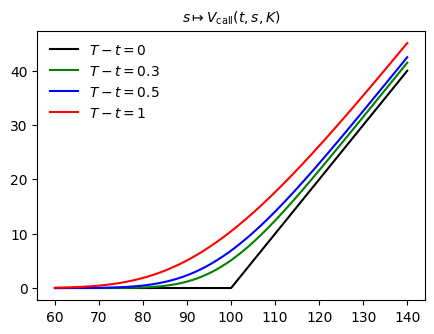
\includegraphics[height=5.2cm]{pic/callprice-s.png}\qquad
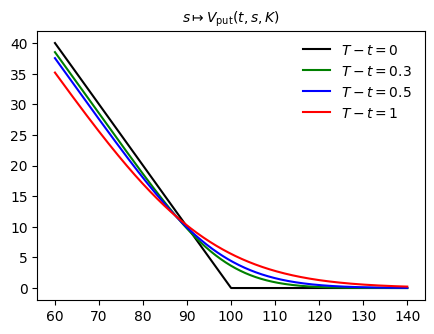
\includegraphics[height=5.2cm]{pic/putprice-s.png}\\
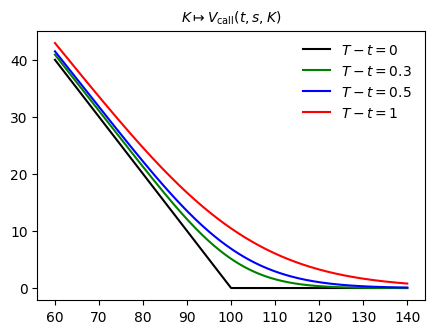
\includegraphics[height=5.2cm]{pic/callprice-k.png}\qquad
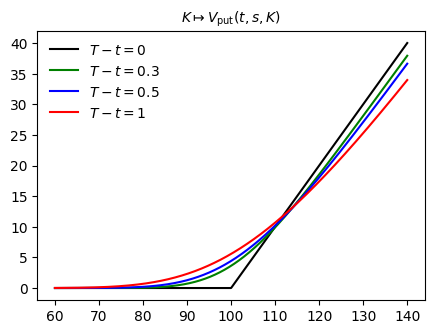
\includegraphics[height=5.2cm]{pic/putprice-k.png}
\caption{Цены опционов колл и пут в модели \bs.}
\label{9:f:bs}
\end{figure}


\subsection{Греки}
\label{9:ss:greeks}

\emph{Греками} (греческими буквами, Greeks) называются производные функции цены опциона по параметрам.

В модели \bs\ цены опционов колл и пут зависят от 5 параметров: цена базового актива $s$, время до экспирации $\tau:=T-t$, страйк $K$, процентная ставка $r$ и волатильность $\sigma$.
Страйк опциона не меняется, поэтому будем рассматривать цены как функции $\VC(s,\tau,r,\sigma)$ и $\VP(s,\tau,r,\sigma)$. 

Выделим следующие часто используемые греки:
\begin{align*}
\text{дельта}\ \Delta &= \frac{\partial V}{\partial s},&
  \text{гамма}\ \Gamma &= \frac{\partial^2 V}{\partial s^2},\\[0.5em]
\text{тета}\ \Theta &= \frac{\partial V}{\partial t} = - \frac{\partial V}{\partial \tau},&
  \text{ро}\ \rho &= \frac{\partial V}{\partial r},\\[0.5em]
\text{вега\footnotemark}\ \mathcal{V} &= \frac{\partial V}{\partial \sigma}.& &
\end{align*}
\footnotetext{Вега "--- это не греческая буква.}

В модели \bs\ греки можно вычислить аналитически.
Формулы приведены в таблице \ref{bs1:t:greeks}, сами вычисления остаются в качестве упражнения.

\begin{table}[h]
\centering
\renewcommand{\arraystretch}{1.25}
\begin{tabular}{|l|c|c|}
\hline
       & Колл & Пут \\\hline
$\Delta$ & $\Phi(d_1)$  & $\Phi(d_1) - 1$ \\\hline
$\Gamma$  & \multicolumn{2}{c|}{$\vphantom{\Bigg|} \dfrac{\phi(d_1)}{s\sigma\sqrt{\tau}}$} \\\hline
$\Theta$   & $\vphantom{\Bigg|} -\dfrac{s\phi(d_1)\sigma}{2\sqrt{\tau}} - rK e^{-r\tau} \Phi(d_2)$ &   $-\dfrac{s\phi(d_1)\sigma}{2\sqrt{\tau}} + rK e^{-r\tau} \Phi(-d_2)$ \\\hline
$\mathcal{V}$   & \multicolumn{2}{c|}{$s\phi(d_1)\sqrt{\tau}$} \\\hline
$\rho$     & $K\tau e^{-r\tau} \Phi(d_2)$  & $-K\tau e^{-r\tau} \Phi(-d_2)$ \\\hline
\end{tabular}
\caption{Греки опционов колл и пут в модели \bs.}
\label{bs1:t:greeks}
\end{table}

С помощью греков можно оценить изменение цены опциона при малом изменении параметров. Действительно, формально раскладывая по формуле Тейлора, получаем
\begin{multline*}
V(s+d s, \tau - d \tau, r+ dr, \sigma+ d\sigma)
\\= V(s,\tau,r,\sigma) + \Delta d s + \Theta d \tau + \mathcal{V} d \sigma + \rho d r + \frac12 \Gamma (d s)^2 + \ldots,
\end{multline*}
где $d$ обозначает малое приращение параметра. (Перед $d\tau$ для удобства стоит знак минус, так как время до экспирации уменьшается с течением календарного времени.)

Для понимания качественного поведения цены при изменении параметров полезно помнить знаки греков (см.~таблицу~\ref{9:t:greeks}).
Например, положительность дельты опциона колл означает, что его цена возрастает при росте цены базового актива; положительность веги обоих опционов означает, что их цена возрастает при увеличении волатильности и \td

\begin{table}[h]
\centering
\renewcommand{\arraystretch}{1.25}
\begin{tabular}{|l|c|c|}
\hline
       & Колл & Пут \\\hline
$\Delta$ & $+$  & $-$ \\\hline
$\Gamma$  & $+$  & $+$ \\\hline
$\Theta$   & $-$\makebox[0pt]{\phantom{$*$}$^*$} & $-$\makebox[0pt]{\phantom{$**$}$^{**}$} \\\hline
$\mathcal{V}$   & $+$  & $+$ \\\hline
$\rho$     & $+$  & $-$ \\\hline
\end{tabular}

\medskip
\parbox{0.78\textwidth}{\footnotesize
* За исключением некоторых опционов в деньгах ($s>K$), когда $r<0$.\\
** За исключением некоторых опционов в деньгах ($s<K$), когда $r>0$.
}

\caption{Знаки греков для опционов колл и пут.}
\label{9:t:greeks}
\end{table}

% \subsection{Другие термины, связанные с опционами}
% \begin{definition}
% Говорят, что опцион колл (или опцион пут) находтс 
% \end{definition}
% \begin{definition}
% Внутренней стоимостью опциона колл (или опциона пут) в момент $t$ называется величина $(S_t-K)^+$ (соответственно, $(K-S_t)^+$).

% Временной стоимостью опциона колл (или опциона пут) в момент $t$ называется величина $\VC_t - (S_t-K)^+$ (соответственно, $(K-S_t)^+$).
% \end{definition}


\section{\difficult\ Другой вывод уравнения Блэка--Шоулза}
Покажем, как можно было бы получить уравнение и формулу \bs\ без привлечения мартингалов, а используя только операции с дифференциалами "--- именно так рассуждали Блэк, Шоулз и Мертон в своих работах.
Будем работать с исходной вероятностной мерой $\P$ и броуновским движением $W$.

Рассмотрим платежное обязательство $X = f(S_T)$.
Ввиду марковости модели разумно предположить, что его цена выражается как функция $V(t,S_t)$. Тогда по формуле Ито имеем
\[
d V(t,S_t) = \Bigl(V'_t(t,S_t) + \mu S_t V'_s(t,S_t) + \frac{\sigma^2}2 S_t^2 V''_{ss}(t,S_t) \Bigr) dt + \sigma S_t V'_s(t,S_t) dW_t.
\]
Подберем теперь самофинансируемую стратегию $\pi=(G,H)$ с таким же стохастическим дифференциалом (и тогда она будет реплицировать платежное обязательство).
Из условия самофинансирования имеем
\[
d V_t^\pi = G_t d B_t + H_t d S_t = rG_t B_t dt + \mu S_t H_t dt + \sigma S_t H_t dW_t. 
\]
Приравнивая коэффициенты при $dt$ и $dW_t$ в этих двух выражениях, получаем
\begin{align*}
&(\text{при}\ dW_t)& &H_t = V'_s(t,S_t),\\
&(\text{при}\ dt)& &r B_t G_t + \mu S_t H_t = V'_t(t,S_t) + \mu S_t V'_s(t,S_t) 
  + \frac{\sigma^2 S_t^2}{2} V''_{ss}(t, S_t).
\end{align*}
Подставляя во второе уравнение $H_t = V'_s(t,S_t)$ и $G_t = V(t,S_t) - H_t S_t$, получаем уравнение Блэка--Шоулза \eqref{9:bs-pde}.
Пользуясь формулой Фейнмана"--~Каца, показывается, что решение уравнения \eqref{9:bs-pde} можно записать в виде \eqref{9:markov-price}.
Уравнение \bs\ можно также решить аналитически, не прибегая к формуле Фейнмана"--~Каца: путем замены переменных оно сводится к уравнению теплопроводности, решение которого известно (детали можно найти в разделе 2 статьи Блэка и Шоулза \cite{BlackScholes73}).


\begin{remark}
Рассуждения в таком выводе уравнения Блэка--Шоулза являются местами нестрогими.
Например, возникают вопросы, почему можно априори утверждать, что функция $V$ является достаточно гладкой, что к ней применима формула Ито; почему из приравнивания коэффициентов при $dt$ и $dW_t$ следует, что цена репликации однозначно определена; и др.
\end{remark}


\summary
\begin{itemize}
\item В модели \bs\ цена рискового актива задается геометрическим броуновским движением со сносом $\mu$ и волатильностью $\sigma$, а цена безрискового актива "--- экспоненциальной функцией $e^{rt}$.

\item В модели \bs\ существует единственная эквивалентная мартингальная мера $\Q$.
Относительно нее процесс цены рискового актива является геометрическим броуновским движением со сносом $r$ и волатильностью $\sigma$.

\item Любое платежное обязательство $X$ такое, что $\E^\Q X^2<\infty$, является реплицируемым, а цену репликации можно найти по формуле $V_t^X = \E^{\Q} (X \mid \F_t)$.

\item Цена платежного обязательства $X=f(S_T)$ имеет вид $V_t^X = V(t,S_t)$, где функция $V(t,s)$ удовлетворяет уравнению \bs\ \eqref{9:bs-pde}, при этом реплицирующая стратегия имеет компоненту $H_t = V'_s(t,S_t)$.

\item Формула \bs\ \eqref{bs1:bs-formula} дает явное выражение для цен европейских опционов колл и пут.

\item Греками называются производные цены опциона по параметрам модели. В модели \bs\ греки вычисляются аналитически (таблица \ref{bs1:t:greeks}).
\end{itemize}

%!TEX root=finmath1.tex
\chapter[Обобщенная модель \bs. Формула Блэка]{Обобщенная модель \bs.\\Формула Блэка}
\label{ch:bs2}
\chaptertoc

В этой лекции мы обобщим модель Блэка--Шоулза: добавим дивиденды и учтем, что безрисковая процентная ставка может быть переменной.
Такая модель, в частности, позволяет рассматривать не только рынки акций, но и валютные рынки.

Также мы получим \emph{формулу Блэка} "--- альтернативное представление формулы \bs, которое более удобно для практического использования.


\section{Обобщение модели \bs}
\subsection{Активы и торговые стратегии}

Будем считать, что рынок задан на фильтрованном вероятностном пространстве $(\Omega, \F, \FF, \P)$ и состоит из безрискового и рискового активов.
Фильтрация порождена броуновским движением $W=(W_t)_{t\in[0,T]}$ и пополнена, $\F = \F_T$.

Цена безрискового актива $B=(B_t)_{t\in[0,T]}$ является неслучайной и задается формулой
\[
B_t = e^{\int_0^t r(u) du},
\]
где $r(t)$ "--- неслучайная, но зависящая от времени, безрисковая процентная ставка.
Будем далее предполагать, что функция $r(t)$ ограничена на $[0,T]$ (и, естественно, измерима).
В дифференциальной форме можно записать
\[
dB_t = r(t) B_t dt, \qquad B_0=1.
\]
Процесс цены рискового актива $S=(S_t)_{t\in[0,T]}$, как и в обычной модели \bs, является геометрическим броуновским движением:
\[
d S_t = \mu S_t dt + \sigma S_t d W_t, \qquad S_0=s_0 >0.
\]
Однако теперь с рисковым активом будет связана еще функция $q(t)$, задающая ставку дивидендной доходности.
Считается, что за промежуток $[t,t+dt]$ этот актив выплачивает дивиденды в размере $q(t)S_t dt$ (строгое понятие будет дано далее в формуле \eqref{10:sf}).
Будем предполагать, что функция $q(t)$ измерима, неотрицательна и ограничена.

\begin{remark}
В реальности дивиденды выплачиваются дискретно "--- например, раз в год, раз в полгода или раз в квартал.
Модель с дискретными дивидендами более трудна; мы ее не рассматриваем.
\end{remark}

\begin{definition}
\emph{Торговой стратегией} в обобщенной модели \bs\ называется пара измеримых согласованных процессов $\pi=(G,H)$, где $G=(G_t)_{t\in[0,T]} \in \PP^1_T$ выражает количество единиц безрискового актива в портфеле, а $H=(H_t)_{t\in[0,T]} \in \PP^2_T$ количество единиц рискового актива. 
\emph{Стоимостью портфеля} стратегии $\pi$ называется процесс 
\[
V_t^\pi = G_t B_t + H_t S_t.
\]
Стратегия называется \emph{самофинансируемой}, если 
\begin{equation}
\label{10:sf}
d V_t^\pi = G_t d B_t + H_t d S_t + q(t) H_t S_t dt.
\end{equation}
\end{definition}

По сравнению с условием самофинансируемости в обычной модели \bs, новым здесь является последнее слагаемое.
Оно выражает размер дивидендов, полученных за <<бесконечно малый>> промежуток времени $dt$.
Можно заметить, что формула \eqref{10:sf} аналогична условию самофинансируемости в модели с дивидендами в дискретном времени (см.\ раздел \ref{gen:s:dividends} в лекции \ref{ch:general}).

\begin{definition}
\emph{Дисконтированной ценой рискового актива с учетом дивидендов} называется процесс 
\[
\tilde S_t = e^{\int_0^t q(u) du} \frac{S_t}{B_t} = e^{\int_0^t (q(u)-r(u)) du} S_t.
\]
\emph{Дисконтированной стоимостью портфеля} стратегии $\pi$ называется процесс 
\[
\tilde V_t^\pi = \frac{V_t^\pi}{B_t} = e^{-\int_0^t r(u) du} V_t^\pi.
\]
\end{definition}

Интерпретация процесс $\tilde S$ здесь такая же, как была в дискретном времени: он представляет собой дисконтированную стоимость портфеля самофинансируемой стратегии $\pi_t=(G_t,H_t)$, которая в начальный момент времени покупает 1 единицу рискового актива и реинвестирует в него дивиденды, \te\ имеет компоненты $G_t\equiv 0$, $H_t = e^{\int_0^t q(u) du}$.

\begin{proposition}
\label{10:p:sf}
Стратегия $\pi$ является самофинансируемой тогда и только тогда, когда
\begin{equation}
\label{10:sf-discounted}
d\tilde V_t^\pi = e^{-\int_0^t q(s)ds} H_t d \tilde S_t.
\end{equation}
\end{proposition}

\begin{proof}
Пусть $\pi$ является самофинансируемой стратегией.
Введем для удобства функцию $D_t = 1/B_t = e^{-\int_0^t r(u)du}$.
Нетрудно видеть, что $dD_t = -r(t) D_t dt$.
Тогда из формулы Ито и условия самофинансируемости находим
\begin{align*}
d \tilde V_t^\pi &= d(D_t V_t^\pi) = D_t(-r(t) V_t^\pi dt + dV_t^\pi) \\
&= D_t (-r(t)V_t^\pi dt + G_tdB_t + H_t d S_t + q(t)H_tS_tdt) \\
&= D_t (-r(t)V_t^\pi dt +r(t)  G_t B_tdt + H_t d S_t + q(t)H_tS_tdt)\\
&= (q(t)-r(t))D_t H_tS_t dt + D_t H_t dS_t.
\end{align*}
Далее введем функцию $U_t = e^{\int_0^t q(s) ds}$, имеющую $dU_t = q(t) U_t dt$.
Заметим, что $d(U_tD_t) = (q(t)-r(t))U_t D_t dt$ (это видно из формулы $U_tD_t = e^{\int_0^t (q(u)-r(u))du}$).
Тогда
\begin{align*}
e^{-\int_0^t q(u)du} H_t d \tilde S_t &= \frac{H_t}{U_t} d(U_tD_tS_t) 
  = \frac{H_t}{U_t} (S_t d(U_tD_t) + U_tD_t dS_t) \\
&= (q(t)-r(t))D_t H_tS_t dt + D_t H_t dS_t. 
\end{align*}
У двух получившихся выражений совпадают правые части.
Значит совпадают и левые, что доказывает формулу \eqref{10:sf-discounted} для самофинансируемых стратегий.

Доказательство в обратную сторону проводится с использованием аналогичных рассуждений (упражнение).
\end{proof}


\subsection{Эквивалентная мартингальная мера}

\begin{theorem}
\label{10:t:emm}
В обобщенной модели \bs\ существует единственная вероятностная мера $\Q\sim\P$, относительно которой процесс $\tilde S$ является мартингалом.
\end{theorem}

\begin{proof}
Пользуясь теоремой Гирсанова, заменим исходную меру $\P$ на такую меру $\Q$, что относительно нее процесс 
\[
W_t^{\Q} = W_t + \int_0^t \frac{\mu+q(u)-r(u)}{\sigma} du
\]
станет броуновским движением (применимость теоремы Гирсанова легко следует из условия Новикова, учитывая ограниченность функций $q(u)$ и $r(t)$).
Тогда $d S_t$ примет вид
\begin{equation}
\label{10:dS}
d S_t = (r(t)-q(t))S_t dt + \sigma S_t d W_t^{\Q},
\end{equation}
что следует из формул $dS_t = \mu S_t dt + \sigma S_t dW_t$ и $d W_t = dW_t^{\Q} - (\mu+q(t)-r(t))/\sigma dt$.

Применяя формулу Ито к процессу $\tilde S_t = U_tD_t S_t$, где $U_t,D_t$ определены в доказательстве предложения~\ref{10:p:sf}, получаем 
\[
d \tilde S_t = \sigma \tilde S_t d W_t^{\Q}.
\]
По новой мере процесс $\tilde S_t$ является геометрическим броуновским движением с нулевым сносом, и, следовательно, является мартингалом.

Доказательство единственности, как и в предыдущей лекции, выходит за рамки курса.
\end{proof}

\begin{definition}
\label{10:d:admissible}
Будем называть стратегию $\pi=(G,H)$ \emph{допустимой}, если $HS \in \L_T^2(Q)$ (эквивалентно, $H\tilde S \in \L_T^2(Q)$), т.е.\ $\E^{\Q} \int_0^T (H_tS_t)^2 dt < \infty$.
\end{definition} 

Далее все стратегии считаются самофинансируемыми и допустимыми, если не оговорено иного.

\begin{proposition}
Для любой самофинансируемой стратегии (допустимость не требуется) имеем
\begin{equation}
\label{10:V-dynamics}
d \tilde V_t^\pi = \sigma e^{-\int_0^t q(s)ds} H_t \tilde S_t d W_t^{\Q},
\end{equation}
или, эквивалентно,
\[
d \tilde V_t^\pi = \sigma H_t \frac{S_t}{B_t} d W_t^{\Q}.
\]
В частности, $\tilde V_t^\pi$ "--- локальный мартингал относительно $\Q$. Если стратегия к тому же допустима, то $\tilde V_t^\pi$ "--- квадратично интегрируемый мартингал.
\end{proposition}

\begin{proof}
Первое утверждение легко следует из подстановки стохастического дифференциала $d \tilde S_t = \sigma \tilde S_t d W_t^{\Q}$ в формулу \eqref{10:sf-discounted}.
Второе утверждение вытекает из свойств интеграла Ито.
\end{proof}


\subsection{Цены платежных обязательств}

Как и в обычной модели \bs, будем отождествлять европейские платежные обязательства с $\F_T$-измеримыми случайными величинами $X$ такими, что $\E^{\Q} X^2 < \infty$.

Приводимая далее теорема и следствие из нее доказывается практически дословно так же, как аналогичные результаты в предыдущей лекции, поэтому доказательства мы опустим.

\begin{theorem}
В обобщенной модели \bs\ любое платежное обязательство имеет единственную реплицирующую стратегию, а цена репликации находится по формуле
\begin{equation}
\label{10:price}
V_t^X = e^{-\int_t^T r(s) ds} \E^{\Q}(X\mid \F_t).
\end{equation}
\end{theorem}

\begin{corollary}
Пусть платежное обязательство $X$ имеет вид $X = f(S_T)$, а функции $f(s)$, $r(t)$, $q(t)$ достаточно ``хорошие''. Тогда $V_t^X = V(t,S_t)$, где
\begin{equation}
\label{10:markov-price}
V(t,s) = e^{-\int_t^T r(u) du} \E^{\Q} (f(S_T) \mid S_t = s)
\end{equation}
является решением уравнения
\[
\left\{
\begin{aligned}
&V'_t(t,s) + (r(t)-q(t))sV'_s(t,s) + \frac{\sigma^2}{2} s^2 V''_{ss}(t,s) = r(t)V(t,s),
  \qquad t\in[0,T), s>0,\\
&V(T,s) = f(s), \qquad s>0.
\end{aligned}
\right.
\]
При этом реплицирующая стратегия задается компонентой $H_t = V'_s(t,S_t)$
\end{corollary}

Поясним, как использовать формулу \eqref{10:markov-price}.
Относительно меры $\Q$ процесс $\tilde S$ является геометрическим броуновским движением, \te\ $\tilde S_t = s_0 e^{\sigma W_t^\Q - \frac{\sigma^2}{2} t}$. Отсюда следует, что процесс $S_t$ имеет вид
\[
S_t = s_0 e^{\int_0^t (r(s)-q(s))ds} e^{\sigma W_t^\Q - \frac{\sigma^2}{2} t},
\]
и, следовательно, можно представить
\[
S_T = S_t e^{\int_t^T (r(s)-q(s) - \frac{\sigma^2}{2})ds} e^{\sigma (W_T^\Q - W_t^\Q)}. 
\]
Тогда вычисление математического ожидания в формуле \eqref{10:markov-price} сводится к вычислению ожидания функции от нормальной случайной величины $W_T^\Q - W_t^\Q \sim N(0,T-t)$, что можно сделать с помощью интегрирования по ее плотности.

Отсюда получаем новый вариант формулы \bs\ для цен европейских опционов колл и пут, а также формулу паритета цен колл-пут.

\begin{corollary}
Для цен европейских опционов колл и пут в обобщенной модели \bs\ Блэка--Шоулза справедливы формулы
\begin{equation}
\label{bs2:bs-formula}
\begin{aligned}
&\VC(t,s) = e^{-\int_t^T q(u) du} s \Phi(d_1) - e^{-\int_t^T r(u) du} K \Phi(d_2), \\
&\VP(t,s) = e^{-\int_t^T r(u) du} K \Phi(-d_2) - e^{-\int_t^T q(u) du} s \Phi(-d_1),\\
&d_1 = \frac{\ln(s/K) + \int_t^T (r(u)-q(u)+\sigma^2/2)du}{\sigma\sqrt{T-t}},\quad
d_2 = d_1 - \sigma\sqrt{T-t}.
\end{aligned}
\end{equation}
Кроме того, для опционов колл и пут с одинаковым временем исполнения и страйком выполняется \emph{паритет цен колл-пут}:
\begin{equation}
\label{10:bs-pc}
\VC(t,s) - \VP(t,s) = e^{-\int_t^T q(u) du} s - e^{-\int_t^T r(u) du} K.
\end{equation}
\end{corollary}


\section{Формула Блэка}

В этом разделе мы перепишем формулу \bs\ в другом виде и получим так называемую \emph{формулу Блэка}.
Они эквивалентны, но формула Блэка более удобна для практического использования.
В качестве вспомогательных результатов мы вычислим цену бескупонной облигации и форвардную цену рискового актива (эти результаты представляют и самостоятельный интерес).

\subsection{Цена бескупонной облигации и форвардная цена акции}

\begin{definition}
\emph{Бескупонная облигация} с временем погашения $T$  отождествляется с платежным обязательством, которое выплачивает детерминированную величину $X$ (\emph{номинал облигации}).
Для цены бескупонной облигации с номиналом $X=1$ в момент времени $t$ будем использовать обозначение $B(t,T)$. 
\end{definition}

\begin{proposition}
В обобщенной модели \bs
\[
B(t,T) = e^{-\int_t^T r(u) du}.
\]
\end{proposition}

\begin{proof}
Очевидно из формулы \eqref{10:price}.
\end{proof}

\begin{definition}
\emph{$T$-форвардной ценой} рискового актива в момент времени $t$ называется $\F_t$-измеримая случайная величина $F_t^T$ такая, что платежное обязательство $X=S_T - F_t^T$ имеет нулевую цену в момент времени $t$.

Если время исполнения $T$ ясно из контекста, то будем говорить просто \emph{форвардная цена} и использовать обозначение $F_t$.
\end{definition}

\begin{proposition}
В обобщенной модели \bs
\[
F_t^T = \E^\Q(S_T\mid \F_t) = S_t e^{\int_t^T (r(u)-q(u)) du}, \qquad
d F_t^T = \sigma F_t^T d W_t^{\Q}.
\]
В частности, форвардная цена является мартингалом относительно $\Q$.
\end{proposition}

\begin{proof}
Имеем
\begin{multline*}
0 = V_t^X = e^{-\int_t^T r(u) du} \E^{\Q}(S_T - F_t^T \mid \F_t) \\= e^{-\int_t^T r(u) du} \E^{\Q} (S_T\mid \F_t) - e^{-\int_t^T r(u) du} F_t^T
= e^{-\int_0^T q(u) du} S_t - e^{-\int_t^T r(u) du} F_t^T,
\end{multline*}
где в последнем равенстве воспользовались тем, что процесс $\tilde S_t = e^{\int_0^t (q(u)-r(u))du} S_t$ является мартингалом относительно меры $\Q$.
Отсюда получаем первую доказываемую формулу.
Применяя формулу Ито и используя выражение для стохастического дифференциала $d S_t$ из \eqref{10:dS}, получаем вторую формулу.
\end{proof}

\subsection{Формулировка и доказательство формулы Блэка}

Пусть $V_t^\text{call}$ и $V_t^\text{put}$ обозначают цены европейских опционов колл и пут.
Будем считать время исполнения $T$ фиксированным и рассмотрим процесс $T$-форвардной цены $F_t$ и цену бескупонной облигации $B(t,T)$. 

\begin{theorem}[формула Блэка]
\label{10:t:black}
Цены опционов колл и пут можно найти в виде $V_t^\text{call} = \VC(t,F_t)$ и $V_t^\text{put} = \VP(t,F_t)$, где функции $\VC(t,f)$ и $\VP(t,f)$ имеют вид
\begin{equation}
\label{bs2:b-formula}
\begin{aligned}
&\VC(t,f) = B(t,T) (f\Phi(d_1) - K\Phi(d_2)), \\
&\VP(t,s) = B(t,T) (K\Phi(-d_2) - f\Phi(-d_1)),\\
&d_1 = \frac{1}{\sigma\sqrt{T-t}} \left(\ln\frac{f}{K} + \frac{\sigma^2}{2}(T-t)\right), \quad
d_2 = d_1 - \sigma\sqrt{T-t}.
\end{aligned}
\end{equation}
\end{theorem}

\begin{proof}
Эти формулы можно получить, если подставить в них выражения для $B(t,T)$ и $F_t$ и показать, что получается формула \bs.

Приведем другой метод доказательства.
Рассмотрим опцион колл (для опциона пут все аналогично). Так как $S_T = F_T$, то
\[
V_t^\text{call} = e^{-\int_t^T r(u) du} \E^{\Q} ((S_T-K)^+ \mid \F_t) 
= B(t,T) \E^{\Q}((F_T - K)^+ \mid \F_t). 
\]
Процесс $F_t$ является геометрическим броуновским движением с нулевым сносом относительно $\Q$, а поэтому для вычисления ожидания в правой части можно воспользоваться стандартной формулой Блэка--Шоулса с нулевой безрисковой ставкой и нулевой дивидендной доходностью (считая, что $F_t$ играет роль цены рискового актива).
Это дает
\[
\E^{\Q}((F_T - K)^+ \mid \F_t) = V(t,F_t),
\]
где $V(t,f)$ -- такая же функция, как в формуле Блэка--Шоулса c $r=q=0$.
Это как раз то, что требовалось показать.
\end{proof}

\noindent
Аналогичным образом можно получить и формулу для паритета колл-пут.

\begin{theorem}[паритет цен колл-пут]
Для опционов колл и пут с одинаковым временем исполнения $T$ и одинаковым страйком $K$ выполнено равенство
\[
V_t^\text{call} - V_t^\text{put} = B(t,T) (F_t - K).
\]
\end{theorem}

\begin{proof}
Можно непосредственно переписать формулу \eqref{10:bs-pc}, либо использовать следующую цепочку равенств:
\begin{multline*}
V_t^\text{call} - V_t^\text{put} = e^{-\int_t^T r(u) du} \E^{\Q} (S_T - K\mid \F_t) \\= 
B(t,T) \E^{\Q} (F_T - K\mid \F_t) = B(t,T) (F_t - K),
\end{multline*}
где в последнем равенстве воспользовались мартингальностью процесса $F_t$. 
\end{proof}

\begin{remark}[о практических применениях]
Формулы \bs и Блэка математически эквивалентны, но для практических применений формула Блэка гораздо удобнее.
Дело в том, что формула \bs\ требует, чтобы были заданы функции $r(t)$ и $q(t)$.
Это означает, что сначала нужно выбрать модель для безрисковой ставки и дивидендов, потом определить ее параметры, и только тогда можно использовать формулу Блэка--Шоулза.

Формула Блэка в этом смысле проще: входящие в нее величины $B(t,T)$ и $F_t$ можно найти из рыночных данных, не используя никакую конкретную модель.
А именно, $B(t,T)$ находится из данных по рынку облигаций%
\footnote{Либо берется облигация с временем погашения в точности $T$, либо, если именно с таким временем погашения облигации не торгуются, то интерполируются цены соседних облигаций.},
а $F_t$ можно найти из паритета цен колл-пут%
\footnote{Форвардные контракты не торгуются на бирже, поэтому для них нет публичных цен.}:
возьмем из рыночных данных цены опционов $V_t^\text{call}$ и $V_t^\text{put}$ для какого-либо страйка $K$, цену $B(t,T)$ посчитаем из данных по облигациям, и тогда получим $F_t = K + (V_t^\text{call} - V_t^\text{put})/B(t,T)$.
\end{remark}


\section{Цены фьючерсов}
\label{bs2:ss:futures}

Покажем, как найти цену фьючерса в обобщенной модели \bs.
Мы будем следовать здесь тем же рассуждениям, что для полной модели рынка в дискретном времени (см.\ раздел \ref{fut:s:complete} в лекции \ref{ch:futures-discrete}) "--- определим цену репликации фьючерса и покажем, что она задается однозначно.

Ради большей общности рассуждений, как и в дискретном времени, будем рассматривать произвольные маржируемые контракты, частным случаем которых является фьючерс.
Маржируемый контракт задается расчетной ценой $X$ в момент экспирации $T$ (фьючерс получается при $X=S_T$).
Далее всегда будем предполагать, что $\E^{\Q} X^2 < \infty$.
Кроме того, будет считаться, что клиринг происходит <<непрерывно>> во времени.

\begin{definition}
\label{bs2:d:fut-price}
\emph{Ценой репликации} маржируемого контракта $X$ называется процесс Ито $F=(F_t)_{t\in[0,T]}$ такой, что $F_T=X$ и существует процесс $\pi_t=(G_t,H_t)$ с компонентами $G\in\PP^1_T$, $H\in\PP^2_T$, причем $HS\in\L_T^2(\Q)$, удовлетворяющий равенствам
\begin{align}
\label{bs2:fut-df}
&dF_t = G_t dB_t + H_tdS_t,\\
\label{bs2:fut-v}
&G_tB_t + H_tS_t = 0,
\end{align}
\end{definition}

\begin{remark}
Равенство \eqref{bs2:fut-df} нужно понимать в интегральном смысле, \te\ $F_t = F_0 + \int_0^t G_u dB_u + \int_0^t H_u d S_u$, где значение $F_0$ не известно.
\end{remark}

Интерпретация равенств \eqref{bs2:fut-df}--\eqref{bs2:fut-v} такая же, как в дискретном времени (определение \ref{fut:d:replication} в лекции \ref{ch:futures-discrete}; более точно, в том определении нужно оставить формулу \eqref{fut:complete-next} "--- аналог формулы \eqref{bs2:fut-v} выше, а формулу \eqref{fut:complete-cur} заменить на разность \eqref{fut:complete-cur} и \eqref{fut:complete-next} "--- аналог \eqref{bs2:fut-df}).
Равенство \eqref{bs2:fut-df} означает, что изменение стоимости портфеля стратегии $\pi$ совпадает с вариационной маржой по контракту.
Равенство \eqref{bs2:fut-v} означает, что стоимость портфеля равна 0, что соответствует тому, что позицию по маржируемому контракту можно открывать и закрывать без издержек.
Отметим, что стратегия $\pi$ не является самофинансируемой "--- приток капитала у нее равен вариационной марже.

\begin{proposition}
В обобщенной модели \bs\ для любого маржируемого контракта $X$ (квадратично интегрируемого по $\Q$) цена репликации существует и задается формулой
\[
F_t = \E^\Q (X\mid \F_t).
\]
В частности, она является квадратично интегрируемым мартингалом относительно $\Q$. 
\end{proposition}

\begin{proof}
Так определенный процесс $F_t$ является квадратично интегрируемым мартингалом по $\Q$ в силу квадратичной интегрируемости $X$.
Согласно теореме о мартингальном представлении, найдется процесс $H'\in \L_T^2(Q)$, для которого 
\[
F_t = F_0 + \int_0^t H_u' d W_u^{\Q}.
\]
Положим $H_t = H_t'/S_t$ и $G_t = -H_t'/B_t$.
Так как $H'\in \L_T^2(\Q)$, то, очевидно, $HS\in\L^2_T(\Q)$, а, следовательно, и $H\in\PP_2^T(\Q)$ и $\G\in\PP^1(\Q)$.
Кроме того, легко видеть, что для $\pi_t=(G_t,H_t)$ выполнены свойства \eqref{bs2:fut-df}--\eqref{bs2:fut-v}.
Значит, $F$ является ценой репликации контракта $X$.

Единственность реплицирующей стратегии следует из того, что для любой реплицирующей стратегии $\pi$ и соответствующей цены $F$ равенства \eqref{bs2:fut-df}--\eqref{bs2:fut-v} влекут
\[
d F_t = -\frac{H_tS_t}{B_t}dB_t + H_tdS_t = \sigma H_t S_t dW_t^\Q,
\]
и, следовательно, $F$ является квадратично интегрируемым мартингалом по $\Q$. По теореме о мартингальном представлении, процесс $\sigma H_t S_t$ однозначно определен.
Значит, однозначно определен и процесс $H_t$. Тогда $G_t$ из него однозначно выражается по формуле \eqref{bs2:fut-v}.
\end{proof}

\begin{corollary}
В обобщенной модели \bs\ $T$-форвардная и $T$"=фьючерсная цена рискового актива совпадают и равны $F_t=\E^\Q(S_T\mid \F_t)$.
\end{corollary}

\begin{remark}
Совпадение форвардных и фьючерсных цен имеет место благодаря тому, что безрисковая процентная ставка считается детерминированной.
Для стохастической ставки это будет не так.
\end{remark}

\begin{remark}
\label{bs2:r:black}
Представляет также интерес \emph{модель Блэка} фьючерсного рынка (часто называемая \emph{моделью Блэка--76} по году публикации работы \cite{Black76}), в которой нет торгуемого базового рискового актива $S_t$, а присутствуют только безрисковый актив и фьючерс, цена которого относительно исходной вероятностной меры $\P$ моделируется геометрическим броуновским движением.

Более подробно модель Блэка изложена в дополнении \ref{ch:black}, где, в частности, выводится \emph{формула Блэка} для цен опционов на фьючерсы.

% Показывается, что в модели Блэка существует единственная ЭММ, относительно которой цена фьючерса является мартингалом (геометрическим броуновским движением с нулевым сносом).
% Тогда цена (премиального) платежного обязательства $X$ вычисляется в виде $V_t=B(t,T)\E^{\Q} (X/B_T\mid\F_t)$.

% В частности, для цен европейских \emph{опционов на фьючерс}%
% \footnote{Опцион на фьючерс "--- это контракт, который дает право покупателю в будущем открыть длинную (опцион колл) или короткую (опцион пут) фьючерсную позицию по фиксированной цене.
% Считается, что экспирация фьючерса происходит не раньше экспирации опционов.}
% получаем формулы $\VC_t = B(t,T)\E^\Q((F_T-K)^+\mid \F_t)$ и $\VP = B(t,T)\E^\Q((K-F_T)^+ \mid \F_t)$,  которые после вычисления математических ожиданий превращаются в точности в фрмулу Блэка.
% Уточним, что здесь $F_T$ обозначает цену фьючерса в момент времени $T$, который экспирируется в момент времени $T'\ge T$. В формулу Блэка вместо параметра $f$ нужно подставлять цену этого фьючерса в момент $t$. Параметр $T'$ в формулу не входит.


\end{remark}


\section{Модель валютного рынка}

Рассмотрим рынок из двух активов "--- денежного счета в \emph{домашней валюте} с безрисковой ставкой $r_d(t)$ и денежного счета в \emph{иностранной валюте} с безрисковой ставкой $r_f(t)$.
Обе ставки детерминированные, а соответствующие процессы цен безрисковых активов имеют вид
\begin{align*}
&d B_t^d = r_d(t) B_t^d dt, \qquad B_0^d = 1,\\
&d B_t^f = r_f(t) B_t^f dt, \qquad B_0^f = 1,
\end{align*}
но при этом $B_t^d$ показывает стоимость в единицах домашней валюты, а $B_t^f$ "--- в единицах иностранной валюты.

Вся случайность в модели связана с обменным курсом.
Будем предполагать, что он моделируется геометрическим броуновским движением
\[
d R_t = \mu R_t dt + \sigma R_t d W_t, \qquad R_0>0,
\]
где $R_t$ выражает стоимость одной единицы иностранной валюты в единицах домашней валюты. 

Как и в модели \bs, считается что фильтрация порождена броуновским движением $W$. 

\begin{definition}
\emph{Торговой стратегией} в модели валютного рынка будем называть пару измеримых согласованных процессов $\pi=(G,H)$, где процесс $G=(G_t)_{t\in[0,T]} \in \PP^1_T$ равен количеству единиц домашнего безрискового актива в портфеле, а $H=(H_t)_{t\in[0,T]} \in \PP^2_T$ -- количеству единиц иностранного безрискового актива. 
\emph{Стоимостью портфеля} стратегии $\pi$ (в домашней валюте) называется процесс 
\[
V_t^\pi = G_t B_t^d + H_t B_t^f R_t.
\]
Стратегия называется \emph{самофинансируемой}, если 
\begin{equation}
\label{10:forex-sf}
d V_t^\pi = G_t d B_t^d + R_t H_t d B_t^f + H_t B_t^f dR_t.
\end{equation}
\end{definition}

Поясним смысл условия самофинансируемости.
Оно является непрерывным аналогом следующего соотношения в дискретном времени (ср.~с формулой на стр.~\pageref{9:self-financing-discrete}):
\[
\Delta V_t^\pi = G_t \Delta B_t^d + R_t H_t\Delta B_t^f + H_tB_t^f\Delta R_t^f.
\]
Первое слагаемое в правой части "--- это приращение стоимости портфеля за счет изменения цены домашнего безрискового актива (эквивалентно, за счет начисления процентов на счет в домашней валюте).
Второе слагаемое "--- приращение стоимости портфеля за счет изменения цены иностранного безрискового актива, выраженное в домашней валюте (умножается на обменный курс).
Третье слагаемое "--- изменение стоимости иностранной части портфеля из-за изменения обменного курса.

\medskip
Далее можно было бы повторить те же рассуждения, что мы проделали для модели Блэка--Шоулза выше (ввести понятие допустимых стратегий, эквивалентной мартингальной меры и \td), но будет проще пойти другим путем и показать, что модель рынка валют можно свести к модели с дивидендами.

Заметим, что стоимость портфеля стратегии $\pi_t=(G_t,H_t)$ будет такая же, как стоимость портфеля стратегии $\pi'=(G_t,H_t')$, где $H_t' = H_tB_t^f$, в обобщенной модели \bs, в которой цена безрискового актива $B_t=B_t^d$, цена рискового актива $S_t=R_t$, безрисковая процентная ставка $r(t) = r_d(t)$, а дивидендная доходность $q(t) = r_f(t)$.
Это вытекает из формулы $V_t^{\pi'} = G_t B_t^d  + H_t' S_t$. 

Следовательно, имеется равенство дифференциалов $d V_t^{\pi'} = d V_t^{\pi}$, а, с другой стороны, формулу \eqref{10:forex-sf} можно переписать в виде
\[
dV_t^{\pi} =  G_t d B_t + q(t) H_t S_t dt + H_t d S_t,
\]
что есть условие самофинансируемости в обобщенной модели \bs.
Таким образом, если стратегия $\pi$ самофинансируемая, то и $\pi'$ самофинансируемая (каждая в своей модели), и наоборот.

Из этого следует, что цена любого платежного обязательства должна совпадать в обеих моделях. 
Отсюда легко получить формулы для цены бескупонной облигации, форвардного и фьючерсного обменного курса и цен опционов в модели валютного рынка.
Сначала дадим соответствующие определения.

\begin{definition}
\emph{Бескупонная облигация} (в домашней валюте) отождествляется с платежным обязательством $X=1$.
\emph{Бескупонная еврооблигация}\footnote{Еврооблигациями называются облигации, номинированные в иностранной валюте. Приставка <<евро>> "--- дань традиции; она не означает, что облигации номинированы в евро.} отождествляется с платежным обязательством $X=R_t$ (\te\ она выплачивает единицу иностранной валюты при погашении).

\emph{$T$-форвардным обменным курсом}%
\footnote{Форвардный контракт -- это соглашение о покупке единицы иностранной валюты в момент времени $T$ по курсу $F_t^T$, который фиксируется в момент $t$.}
в момент времени $t$ называется $\F_t$"=измеримая случайная величина $F_t^T$ такая, что платежное обязательство $X=R_T - F_t^T$ имеет нулевую цену в момент времени $t$. \emph{Валютным фьючерсом} называется фьючерс на поставку единицы иностранной валюты в момент экспирации, отождествляемый с маржируемым контрактом с расчетной ценой $F_T=R_T$.

\emph{Валютные опционы колл и пут} (европейского типа) с временем исполнения $T$ и страйком $K$ дают право купить/продать единицу иностранной валюты в момент $T$ по курсу $K$ и отождествляются с платежными обязательствами $X= (R_T - K)^+$ и $X=(K-R_T)^+$.
\end{definition}

Теперь, сводя модель валютного рынка к обобщенной модели \bs, получаем следующий результат.
\begin{proposition}
В рассматриваемой модели валютного рынка
\begin{itemize}
\item цена бескупонной домашней облигации равна $B_d(t,T) = e^{-\int_t^T r_d(u) du}$;
\item цена бескупонной еврооблигации равна $B_f(t,T) = R_t e^{-\int_t^T r_f(u) du}$ (в единицах домашней валюты);
\item $T$-форвардный обменный курс и цена фьючерса с моментом экспирации $T$ совпадают и равны $F_t^T = R_t e^{\int_t^T (r_d(u)-r_f(u)) du}$;
\item формула Блэка для цен опционов имеет такой же вид, как в теореме~\ref{10:t:black}.
\end{itemize}
\end{proposition}


\summary
\begin{itemize}
\item В обобщенной модели \bs\ процентная ставка $r(t)$ неслучайна, но зависит от времени, а рисковый актив выплачивает дивиденды со ставкой доходности $q(t)$. Цены опционов колл и пут можно найти из обобщенной формулы \bs\ \eqref{bs2:bs-formula}.

\item Формула Блэка \eqref{bs2:b-formula} позволяет переписать формулу \bs\ через форвардную цену рискового актива и цену бескупонной облигации таким образом, что в нее в явном виде не входят безрисковая ставка и дивидендная доходность.

\item Цена бескупонной облигации с номиналом 1 равна $B(t,T) = e^{-\int_t^t r(s) ds}$, а $T$-форвардная цена рискового актива равна $F_t^T = S_t e^{\int_t^T (r(u)-q(u)) du}$, причем последняя является мартингалом относительно ЭММ. 

\item В модели валютного рынка присутствуют два безрисковых актива "--- в домашней и зарубежной валюте "--- с разными процентными ставками $r_d(t)$ и $r_f(t)$.
Обменный курс задается геометрическим броуновским движением. 

\item Для опционов на зарубежную валюту верна формула Блэка, в которую нужно подставить цену бескупонной домашней облигации $B_d(t,T) = e^{-\int_t^t r_d(s) ds}$ и $T$-форвардный обменный курс $F_t^T = R_t e^{\int_t^T (r_d(u)-r_f(u)) du}$.
\end{itemize}

%!TEX root=finmath1.tex
\chapter{Подразумеваемая волатильность}
\label{ch:iv}
\chaptertoc

\emph{Подразумеваемая волатильность} "--- это такое значение параметра волатильности $\sigma$, которое рынок закладывает в цены опционов.
В этой лекции мы обсудим метод вычисления подразумеваемой волатильности из рыночных цен европейских опционов, а также увидим, что в реальных данных она различается для опционов с различными страйками и временем экспирации.
Этот факт, в частности, означает, что модель \bs\ на практике не верна.

\section{Понятие подразумеваемой волатильности}
\subsection{Определение и комментарии}

Далее мы будем работать с ценами европейских опционов колл и пут, вычисляемыми по формуле Блэка.
В этой формуле цена зависит от 5 аргументов: время до экспирации $T$ (текущий момент времени $t$ будет всегда считаться нулевым), страйк $K$, $T$-форвардная цена $F$, цена бескупонной облигации $B$ c погашением в момент $T$ и волатильность $\sigma$.
Значения первых четырех аргументов известны либо из спецификации самого опциона ($T$, $K$), либо из рыночных данных ($F$, $B$ "--- ниже будет объяснено, как их получить).
Значение волатильности $\sigma$ является модельным параметром и должно быть оценено.

С другой стороны, рыночные цены опционов известны (из котировок на бирже), поэтому на формулу Блэка 
\begin{equation}
\label{iv:equation}
\VC = \VC(T,K,F,B,\sigma) \qquad(\text{или}\ \VP = \VP(T,K,F,B,\sigma))
\end{equation}
можно посмотреть как на уравнение, в котором $\sigma$ является единственной неизвестной величиной.

\begin{definition}
\emph{Подразумеваемой} (также \emph{предполагаемой}, \emph{вмененной}, \emph{implied volatility}) \emph{волатильностью} $\hat\sigma$ называется такое значение параметра $\sigma$, что при подстановке его в формулу Блэка, цена опциона, вычисленная по этой формуле, совпадает с рыночной ценой.
\end{definition}

Таким образом, $\hat\sigma$ "--- это значение параметра волатильности, которое <<рынок закладывает>> в расчет цены опциона.

Эмпирическим фактом, наблюдаемым для всех активов, является то, что значение подразумеваемой волатильности оказывается разным для различных опционов на один и тот же базовый актив.
В качестве примера на рис.~\ref{11:f:iv} показаны подразумеваемые волатильности опционов на индекс S\&P 500.
Четко видна зависимость подразумеваемой волатильности и от $T$, и от $K$.

\begin{figure}[h]
\centering
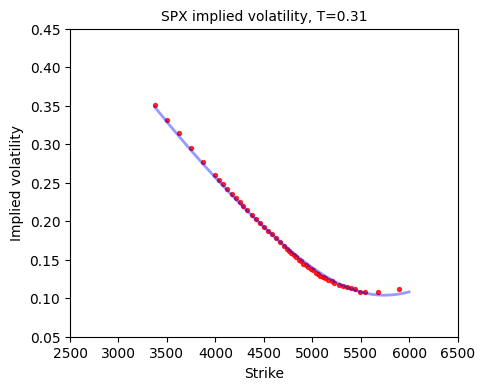
\includegraphics[height=3.7cm]{pic/iv-3m.png}
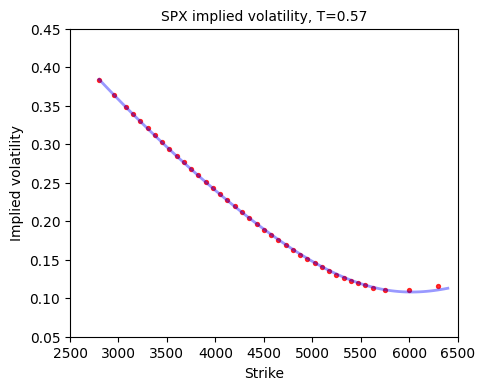
\includegraphics[height=3.7cm]{pic/iv-6m.png}
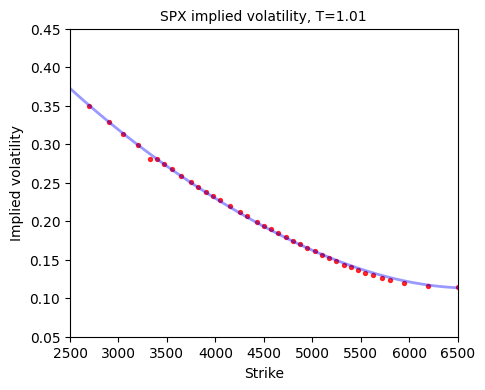
\includegraphics[height=3.7cm]{pic/iv-1y.png}
\caption{Подразумеваемые волатильности опционов на индекс S\&P 500 (данные на 6.03.2024). Три графика соответствуют трем разным значениям времени до экспирации.}
\label{11:f:iv}
\end{figure}

Это обстоятельство, в частности, означает что модель модель \bs\ на практике не верна: если бы цены всех опционов на один и тот же базовый актив вычислялись по формуле Блэка (или \bs), то $\hat\sigma$ была бы одинаковой для всех значений $T,K$ и равнялась бы параметру $\sigma$ геометрического броуновского движения.

Тем не менее, это не означает, что модель Блэка--Шоулза не нужна.
На самом деле, модель \bs\ используется для \emph{взаимнооднозначного преобразования из цен опционов в подразумеваемую волатильность}.

Оказывается, что с подразумеваемой волатильностью гораздо удобнее работать, чем с ценами опционов, так как на цену оказывают влияние еще и параметры $T,K,F,B$, в то время как волатильность очищена от этих факторов. 
Кроме того, для трейдеров значение волатильности гораздо информативнее отражает насколько дорог или дешев опцион, чем сами цены: из фразы <<волатильность опциона 50\%>> качественно понятно, что опцион дорогой, даже если не называть базовый актив; а из фразы <<цена опциона 10 долларов>> ничего не ясно без указания остальных параметров.
Наконец, совокупность значений подразумеваемой волатильности (так называемая \emph{поверхность волатильности} "--- см.~далее) используется для подгонки параметров более продвинутых моделей цен активов и является важнейшим <<входным параметром>> для них. 

\begin{remark}
Можно также вычислить \emph{историческую волатильность} "--- по прошлым ценам рискового актива статистически оценить коэффициент $\sigma$ геометрического броуновского движения.
Историческая волатильность качественно отличается от подразумеваемой в том, что, во-первых, историческая волатильность <<смотрит>> в прошлое, а подразумеваемая "--- в будущее. Во-вторых, историческая волатильность "--- это число, в то время как подразумеваемая волатильность "--- это функция от страйка и времени до экспирации опциона.
\end{remark}

Докажем полезный вспомогательный результат, который показывает, что подразумеваемая волатильность европейских опционов колл и пут совпадает.

\begin{proposition}
Если на рынке выполняется паритет цен колл-пут%
\footnote{Напомним, что паритет цен колл-пут выполняется в любой безарбитражной теоретической модели.
В реальности он тоже обычно выполняется (с точностью до погрешности, возникающей из-за транзакционных издержек).}
$($т.е.\ $\VC - \VP = B(F-K)$$)$, то значение $\hat\sigma$, вычисленное для опциона колл, совпадает со значением $\hat\sigma$, вычисленным для опциона пут с таким же страйком и временем до экспирации.
\end{proposition}

\begin{proof}
Пусть $\hat\sigma_c$ "--- подразумеваемая волатильность опциона колл, а $\hat\sigma_p$ "--- подразумевая волатильность опциона пут с такими же $T$ и $K$.
Предположим, от противного, что $\hat\sigma_c\neq \hat\sigma_p$. 

Для любого $\sigma \neq \hat\sigma_p$ имеем $\VP(\sigma) \neq \VP(\hat\sigma_p)$ так как функция $\VP$ строго возрастает по $\sigma$, что следует из положительности ее производной по $\sigma$. 
Но так как $\VC(\hat\sigma_c) - \VP(\hat\sigma_c) = B(F-K)$ из-за того, что паритет колл-пут выполняется в модели \bs, то $\VC(\hat\sigma_c) - \VP(\hat\sigma_p) \neq B(F-K)$.
В левой части здесь стоит разность рыночных цен опционов колл и пут (по определению подразумеваемой волатильности), поэтому получается, что на рынке паритет колл-пут не выполнен. 
Противоречие.
\end{proof}

\begin{definition}
\label{iv:d:surface}
Для заданного базового актива \emph{поверхностью подразумеваемой волатильности}  называется функция $\hat\sigma(T,K)$ с аргументами $T,K> 0$, выражающая зависимость подразумеваемой волатильности от времени до экспирации  и страйка.

\emph{Улыбкой подразумеваемой волатильности} для заданного времени $T>0$ называется функция $K\mapsto\sigma(T,K)$, \te\ одно сечение поверхности волатильности.
\end{definition}

Далее для краткости будем говорить просто <<поверхность волатильности>> или <<улыбка полатильности>>, опуская слово <<подразумеваемой>>.

\begin{remark}
Величина $T$ обычно выражается в годах, $K$ "--- в единицах валюты, а $\hat\sigma$ "--- безразмерная величина или выражается в процентах.
Типичные значения волатильности "--- от 0.1 до 0.5, в зависимости от актива, параметров $T,K$ опциона и ожидания риска у трейдеров.
При изменении масштаба по времени в $s$ раз волатильность следует изменить в $\sqrt{s}$ раз, \te, например, при выражении времени в месяцах типичные значения $\hat\sigma$ будут от $0.1/\sqrt{12}$ до $0.5/\sqrt{12}$.
\end{remark}

\begin{remark}
Строго говоря, волатильность $\sigma\hat(T,K)$, вычисленная из рыночных цен опционов, еще не является функцией, так как на рынке имеется лишь конечное число комбинаций $T$ и $K$ для торгуемых опционов.
Для того, чтобы получить функцию, нужно провести интерполяцию и экстраполяцию данных.
Далее мы будем считать, что эти операции уже проведены (как это правильно сделать "--- отдельная задача, которая в курсе не рассматривается).
\end{remark}


\subsection{Необходимое и достаточное условие существования подразумеваемой волатильности}
Далее будем считать, что $T>0$ и $K>0$.

\begin{proposition}
\label{iv:p:existence}
Подразумеваемая волатильность существует (\te\ уравнение \eqref{iv:equation} имеет единственное решение $\hat\sigma$) тогда и только тогда, когда
\begin{equation}
\label{iv:call-bounds}
B(F-K)^+ < \VC < BF,
\end{equation}
или, эквивалентно,
\begin{equation}
\label{iv:put-bounds}
B(K-F)^+ < \VP < BK
\end{equation}
\end{proposition}

\begin{proof}
Докажем только утверждение для опционов колл, для пут оно доказываетя аналогично.
Зафиксируем $T,K,F,B$ и будем рассматривать цену опциона колл как непрерывную функцию $V(\sigma) = \VC(T,K,F,B,\sigma)$.

Заметим, что $V$ строго возрастает, так как $V'(\sigma)>0$ для всех $\sigma>0$ (это свойство  положительности веги опциона; см.~раздел \ref{9:ss:greeks} в лекции \ref{ch:bs}).
Кроме того, 
\[
\lim_{\sigma\to\infty} V(\sigma) = BF, \qquad
\lim_{\sigma\to 0} V(\sigma) = \begin{cases}
B(F-K), &f > K,\\
0, &f\le K,
\end{cases}
\]
в чем нетрудно убедиться, переходя к пределу в формуле Блэка.
Теперь видно, что доказываемое утверждение следует из теоремы о промежуточном значении строго монотонной непрерывной функции.
\end{proof}

Отметим, что ограничения \eqref{iv:call-bounds} и \eqref{iv:put-bounds} должны выполняться в любой безарбитражной модели, а не только в модели \bs, что делает возможным вычисление подразумеваемой волатильности для любых (безарбитражных) рыночных данных, не далая конкретных предположений о модели рынка.

(Упражнение: покажите, что если $\VC<B(F-K)^+$ или $\VC> BF$, то можно построить арбитражную возможность; если дополнительно предположить, что цена $S_T$ принимает значения в любом интервале $(a,b)\subset\R_+$ с положительной вероятностью, то арбитражная возможность найдется и в случаях $\VC=B(F-K)^+$ и $\VC=BF$.
Аналогично для опционов пут.)




\section{Вычисление подразумеваемой волатильности}

\subsection{Какие данные использовать?}

Задача вычисления подразумеваемой волатильности состоит в том, чтобы для набора времен исполнения и страйков $(T_i,K_i)$ вычислить значения $\hat\sigma_i = \hat\sigma(T_i,K_i)$. 

Для каждой пары $(T_i,K_i)$, как правило, в рыночных данных имеются как минимум четыре цены: цены бид и аск%
\footnote{\emph{Бид} (bid) -- лучшая заявка на покупку в стакане заявок (с наиболее дорогой ценой), \emph{аск} (ask) -- лучшая заявка на продажу (с наиболее дешевой ценой). Цена бид всегда меньше цены аск.
Если инструмент неликвидный, то стакан заявок может содержать только одну из цен бид/аск или вообще быть пустым.}
опционов колл и цены бид и аск опционов пут; также обычно присутствуют цены последних сделок (если сделки были).
На практике для вычисления $\hat\sigma$ применяются следующие соображения.

\begin{itemize}
\item Используют только опционы АTMF и OTMF%
\footnote{
ATMF (at-the-money forward, опцион \emph{на} деньгах) -- опцион со страйком равным форвардной цене, $K=F$.
OTMF (out-of-the-money forward, опцион \emph{вне} денег) -- опцион колл с $K>F$ или опцион пут с $K<F$.
ITMF (in-the-money forward, опцион \emph{в} деньгах) -- опцион колл с $K<F$ или опцион пут с $K>F$.
 
Термины без буквы F (ATM, ITM, OTM) означают то же самое с тем лишь различием, что $K$ сравнивается с текущей ценой базового актива, а не с форвардной ценой.} (т.е.\ колл для $K\ge F$ и пут для $K\ge F$; если какой-то страйк попадает на форвардную цену, то можно взять среднее значение подразумеваемой волатильности для колл и пут), что связано с тем, что такие опционы более ликвидны, чем ITMF. 

\item Вместо цен бид и аск используют цену \emph{мид} (среднее цен бид и аск).
Если нужна особая точность или спред цен бид-аск большой, то оперируют с двумя поверхностями волатильности: по ценам бид и по ценам аск.

\item Не используют цены последних сделок, особенно по далеким от ATMF опционам, так как с момента последней сделки могло пройти много времени.
\end{itemize}



Далее нужно вычислить цену бескупонной облигации $B$ и форвардную цену $F$.
Про цены бескупонных облигаций более подробно рассказано в следующем разделе, а сейчас остановимся на форварде.
На практике $T$-форвардную цену (для каждого $T$ свою) вычисляют из цен опционов через паритет колл-пут, а именно,
\[
F = \frac{\VC - \VP}{B} + K.
\]
В теории паритет колл-пут должен выполняться для любого страйка, но для практических вычислений лучше взять страйк наиболее близкий к значению $F$.
Так как само значение $F$ еще не вычислено, то можно взять тот страйк, у которого разность цен опционов колл и пут минимальна (для опционов ATMF имеем $\VC=\VP$, что видно из формулы \eqref{11:black} c $x=0$).

\medskip
В итоге, имея цены опционов колл и пут, форвардные цены и цены бескупонных облигаций, можно численно находить значение подразумеваемой волатильности из решения уравнения \eqref{iv:equation}.
Существуют различные программные пакеты для эффективного решения этой задачи%
\footnote{Один из наиболее эффективных алгоритмов "--- ``Let's be rational'' Питера Джекела \cite{Jaeckel15}.
На сайте автора имеется эталонная реализация на C: \url{www.jaeckel.org/LetsBeRational.7z}.
Существует также библиотека для Python: \url{https://github.com/vollib/py_vollib}.}.
В разделе \ref{iv:ss:algorithm} будет описан один алгоритм, который, несмотря на свою простоту, работает достаточно хорошо.

\begin{remark}
Вычислять подразумеваемую волатильность посредством обращения формулы Блэка следует только для европейских опционов.
Вычисление подразумеваемой волатильности для американских опционов является более трудной задачей; мы кратко коснемся ее в лекции \ref{ch:american-continuous}.
\end{remark}


\subsection{Кривая бескупонной доходности}

Для практических применений нужно брать значение процентной ставки $r(t)$ исходя из того, под какую ставку может финансироваться трейдер.
Для исследовательских применений можно использовать процентные ставки, полученные из кривой доходности по государственных облигациям "--- они легко доступны и дают хорошую точность расчетов. 
Дадим соответствующие определения.

Будем считать, что текущий момент времени $t=0$, тогда $T$ будет обозначать время до погашения облигации. 

\begin{definition}
\emph{Кривой бескупонной доходности} называется функция $y(t)$ такая, что рыночная стоимость бескупонной облигации с временем до погашения $T$ может быть найдена по формуле $B(0,T) = e^{-y(T) T}$ (т.е.\ $y(t) = -\frac 1t \ln B(0,t)$).
\end{definition}

Смысл определения бескупонной доходности в том, что она показывает какой должна была бы быть постоянная процентная ставка, чтобы цена бескупонной облигация в модели с такой ставкой равнялась рыночной цене.

Если имеется кривая бескупонной доходности, то для вычисления цен опционов по формуле Блэка в момент времени $t=0$ нужно использовать величины $B(0,T) = e^{-y(T) T}$.
Время $T$ обычно измеряется в годах. 

\begin{remark}
\emph{Краткосрочной (овернайт) ставкой} называется ставка, по которой участники рынка могут одолжить или взять деньги на один день.

В модели \bs\ краткосрочная ставка выражается функцией $r(t)$. 
Если считать, что $r(t)$ неслучайна, то, используя формулу $B(0,T) = e^{-\int_0^T r(t) dt}$, из кривой бескупонной доходности находим, что $r(t) = (y(t)t)'$.
\end{remark}

Для построения кривой бескупонной доходности используются государственные облигации, так как их можно считать практически безрисковыми (государство может напечатать деньги, чтобы расплатиться по облигациям).
В реальности бескупонные облигации торгуются лишь для малого числа значений $T$.
Чтобы получить кривую бескупонной доходности для длинного горизонта времени (до 30 лет), во-первых, используют стандартную процедуру нахождения эквивалентной бескупонной доходности для облигаций с купонами (\emph{бутстрэп}) и, во-вторых, проводят интерполяцию дискретного набора данных. 

Стандартным методом интерполяции является \emph{модель Нельсона"--~Сигеля"--~Свенсона}, которая представляет кривую бескупонной доходности в виде
\[
y(t) = \beta_0 + \beta_1\frac{1-e^{-\frac{t}{\tau_1}}}{\frac t{\tau_1}}
  + \beta_2 \left( \frac{1-e^{-\frac{t}{\tau_1}}}{\frac t{\tau_1}} - e^{-\frac t{\tau_1}}\right)
  + \beta_3 \left( \frac{1-e^{-\frac{t}{\tau_2}}}{\frac t{\tau_2}} - e^{-\frac t{\tau_2}}\right),
\]
где $\beta_1,\beta_2,\beta_3,\tau_1,\tau_2$ -- параметры модели, которые оценивают так, чтобы получаемая кривая бескупонной доходности наилучшим образом соответствовала рыночным данным.

Параметры модели Нельсона"--~Сигеля"--~Свенсона для рынка США можно найти на сайте Федерального резерва\footnote{\url{https://www.federalreserve.gov/data/nominal-yield-curve.htm}}, там же более подробно описана методология их вычисления.
Кривую бескупонной доходности для российского рынка и коэффициенты модели (используется другая, но аналогичная модель) можно найти на сайте Московской биржи\footnote{\url{https://www.moex.com/a3642}}.

Рис.~\ref{11:f:zcb} показывает пример того, как выглядит кривая бескупонной доходности для американского рынка.

\begin{figure}[h]
\centering
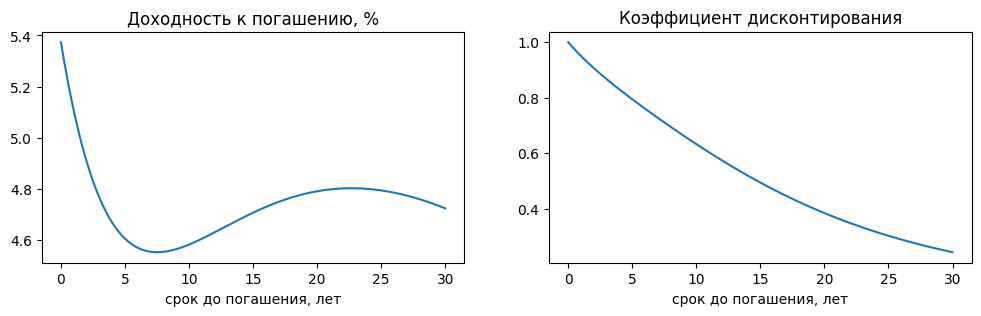
\includegraphics[width=\textwidth]{pic/yield-curve.png}
\caption{Кривая бескупонной доходности в США. Данные на 24.04.2024.}
\label{11:f:zcb}
\end{figure}


\subsection{\difficult\ Численный алгоритм}
\label{iv:ss:algorithm}
В этом разделе мы опишем численный метод решения уравнения \eqref{iv:equation}, основанный на идеях статьи \cite{Jaeckel06}.
В его основе лежит классический итерационный метод Ньютона нахождения корня уравнения, причем будет показано, что он гарантированно сходится при специальном выборе начального приближения. 

Для начала приведем уравнение \eqref{iv:equation} к более удобному виду.
Будем считать, что $T>0$.
Пусть $V$ обозначает цену опциона колл или пут (в зависимости от того, какой из них рассматривается).
Введем обозначения
\[
y = \ln\frac FK, \qquad
p = \frac{V}{B\sqrt{FK}}, \qquad
x = \hat\sigma\sqrt{T},\qquad
\theta=\begin{cases}
  1 &\text{для опциона колл},\\
  -1 &\text{для опциона пут}.
\end{cases}
\]
Подставляя эти обозначения в формулу Блэка, можно переписать уравнение \eqref{iv:equation} так:
\begin{equation}
\label{11:black}
\theta\left(e^{\frac y2}\Phi\left(\theta\left(\frac yx + \frac x2\right)\right) - e^{-\frac y2}\Phi\left(\theta \left(\frac yx - \frac x2\right)\right)\right) - p=0.
\end{equation}
Также нетрудно преобразовать условие предложения \ref{iv:p:existence} и получить, что решение уравнения \eqref{11:black} существует и единственно тогда и только тогда, когда
\begin{equation}
\label{11:exist}
\theta \I(\theta y>0) (e^{\frac y2} - e^{-\frac y2}) < p < e^{\theta \frac y2}.
\end{equation}

Если выполнено условие \eqref{11:exist}, то можно найти $\hat\sigma$ численно.
Напомним, что общий метод Ньютона численного решения уравнения $f(x) = 0$ состоит в построении последовательности приближений $x_n$ таких, что при некоторых условиях на функцию $f$ имеет место сходимость $x_n\to x^*$, где $x^*$ "--- решение.

Начальное приближение $x_0$ выбирается произвольно (но от его выбора может зависеть сходимость метода).
Следующие приближения находятся по формуле
\[
x_{n+1} = x_n - \frac{f(x_n)}{f'(x_n)}.
\]
Смысл метода Ньютона в том, что в точке $x_n$ строится касательная к графику функции $f$, и новое приближение $x_{n+1}$ выбирается как точка пересечения этой касательной с осью абсцисс.
Обычно прекращают итерации, когда разность $|x_{n+1}-x_n|$ становится меньше заданной точности.
На рис.~\ref{iv:f:newton} изображен пример итераций метода Ньютона.

\begin{figure}[h]
\centering
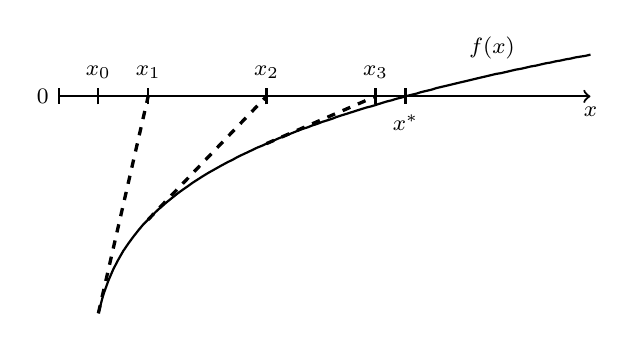
\begin{tikzpicture}[xscale=2.5,yscale=5]
\draw[thick,->] (-0.2,0) node[left] {\footnotesize $0$} --(2.5,0) node[below] {\footnotesize $x$};
\draw[thick] (-0.2,0.02)--(-0.2,-0.02);
\draw[thick] (0,-0.02) -- (0,0.02) node[above] {\footnotesize $x_0$};
\draw[thick] (0.253,-0.02) -- (0.253,0.02)  node[above] {\footnotesize $x_1$};
\draw[thick] (0.854,-0.02) -- (0.854,0.02) node[above] {\footnotesize $x_2$};
\draw[thick] (1.408,-0.02) -- (1.408,0.02) node[above] {\footnotesize $x_3$};
\draw[thick] (1.5605,0.02) -- (1.5605,-0.02) node[below] {\footnotesize $x^*$};
\draw (2,0.07) node[above] {\footnotesize $f(x)$};
% f(x) = (x+0.05)**0.2-1.1, x \in [0, 2.5]
\draw[thick] (0.000,-0.551)--(0.025,-0.504)--(0.051,-0.468)--(0.076,-0.439)--(0.101,-0.415)--(0.126,-0.393)--(0.152,-0.374)--(0.177,-0.357)--(0.202,-0.341)--(0.227,-0.326)--(0.253,-0.313)--(0.278,-0.300)--(0.303,-0.288)--(0.328,-0.277)--(0.354,-0.266)--(0.379,-0.256)--(0.404,-0.246)--(0.429,-0.237)--(0.455,-0.228)--(0.480,-0.219)--(0.505,-0.211)--(0.530,-0.203)--(0.556,-0.195)--(0.581,-0.188)--(0.606,-0.181)--(0.631,-0.174)--(0.657,-0.167)--(0.682,-0.161)--(0.707,-0.154)--(0.732,-0.148)--(0.758,-0.142)--(0.783,-0.136)--(0.808,-0.130)--(0.833,-0.125)--(0.859,-0.119)--(0.884,-0.114)--(0.909,-0.108)--(0.934,-0.103)--(0.960,-0.098)--(0.985,-0.093)--(1.010,-0.088)--(1.035,-0.083)--(1.061,-0.079)--(1.086,-0.074)--(1.111,-0.070)--(1.136,-0.065)--(1.162,-0.061)--(1.187,-0.057)--(1.212,-0.052)--(1.237,-0.048)--(1.263,-0.044)--(1.288,-0.040)--(1.313,-0.036)--(1.338,-0.032)--(1.364,-0.028)--(1.389,-0.025)--(1.414,-0.021)--(1.439,-0.017)--(1.465,-0.013)--(1.490,-0.010)--(1.515,-0.006)--(1.540,-0.003)--(1.566,0.001)--(1.591,0.004)--(1.616,0.007)--(1.641,0.011)--(1.667,0.014)--(1.692,0.017)--(1.717,0.021)--(1.742,0.024)--(1.768,0.027)--(1.793,0.030)--(1.818,0.033)--(1.843,0.036)--(1.869,0.039)--(1.894,0.042)--(1.919,0.045)--(1.944,0.048)--(1.970,0.051)--(1.995,0.054)--(2.020,0.057)--(2.045,0.059)--(2.071,0.062)--(2.096,0.065)--(2.121,0.068)--(2.146,0.070)--(2.172,0.073)--(2.197,0.076)--(2.222,0.078)--(2.247,0.081)--(2.273,0.084)--(2.298,0.086)--(2.323,0.089)--(2.348,0.091)--(2.374,0.094)--(2.399,0.096)--(2.424,0.099)--(2.449,0.101)--(2.475,0.103)--(2.500,0.106);
%
\draw[very thick,dashed] (0.000, -0.551) -- (0.253,0);
\draw[very thick,dashed] (0.253, -0.313) -- (0.854,0);
\draw[very thick,dashed] (0.854, -0.120) -- (1.408,0);
\end{tikzpicture}
\caption{Решение уравнения методом Ньютона.}
\label{iv:f:newton}
\end{figure}

\begin{proposition}
\label{iv:p:newton}
Предположим, что функция $f(x)$ непрерывно дифференцируема, строго возрастает и вогнута на  отрезке $[x_0,x^*]$, где $f(x^*)=0$. 
Тогда метод Ньютона с начальным приближением $x_0$ сходится к $x_*$.

Аналогичное утверждение верно, если $f$ выпукла на отрезке $[x^*,x_0]$.
\end{proposition}

\begin{proof}
Докажем только первое утверждение; второе аналогично.
В силу возрастания $f$, имеем $f(x_0) < 0$.
Так как график вогнутой функции лежит ниже любой своей касательной, то касательная, проведенная в точке $x_0$, должна пересечь ось абсцисс между точками $x_0$ и $x_*$.
Используя то же самое рассуждение, по индукции получаем, что $x_{n-1} < x_n < x_*$ для всех $n$.

Таким образом, последовательность $x_n$ возрастает и ограничена сверху значением $x_*$.
Следовательно, она имеет предел $\tilde x$.
Покажем, что $\tilde x=x_*$.
Предположим, от противного, что $\tilde x < x_*$.
Тогда найдутся такие $\epsilon,\delta>0$, что $f(x)/f'(x) \le -\epsilon$ при $x \in (\tilde x, \tilde x+\delta)$ (в силу того, что $f(x)$ отрицательна в окрестности $\tilde x$, а $f'(x)$ ограничена и положительна в силу своей непрерывности и возрастания $f(x)$).
Но так как $x_{n+1} - x_n = -f(x_n)/f'(x_n)$, то получаем противоречие со сходимостью последовательности $x_n$. Значит, $\tilde x = x_*$.  
\end{proof}

\begin{proposition}
Пусть выполнено условие \eqref{11:exist}.
Обозначим за $x^*$ решение уравнения \eqref{11:black}.
Тогда справедливы следующие утверждения.

1. Если $y=0$ (опцион ATMF), то 
\begin{equation}
\label{11:atm}
x^* = 2 \Phi^{-1}\left(\frac{1+p}{2}\right),
\end{equation}
где $\Phi^{-1}$ "--- обратная к стандартной нормальной функции распределения.

2. Если $y\neq 0$, то правая часть уравнения \eqref{11:black}, рассматриваемая как функция от $x$, имеет точку перегиба $x_0 = \sqrt{2|y|}$ и является выпуклой на интервале $(0,x_0)$ и вогнутой на $(x_0,\infty)$, а метод Ньютона с начальным приближением $x_0 = \sqrt{2|y|}$ сходится к $x^*$.
\end{proposition}

\begin{proof}
Формула \eqref{11:atm} очевидно следует из подстановки $y=0$ в \eqref{11:black}.
Докажем второе утверждение.
Обозначим за $f(x)$ правую часть \eqref{11:black}.
Непосредственно вычисляется
\[
f'(x) = \frac{1}{\sqrt{2\pi}} e^{-\frac12\left(\frac{y^2}{x^2} + \frac{x^2}4\right)},\qquad
f''(x) = \frac{x}{\sqrt{2\pi}} e^{-\frac12\left(\frac{y^2}{x^2} + \frac{x^2}4\right)}
  \left(\frac{y^2}{x^4} - \frac14\right).
\]
Видно, что $f'>0$, и, следовательно, $f$ строго возрастает.
Кроме того, $f''(x) > 0$ при $x < x_0$ и $f''(x) < 0$ при $x > x_0$.
Таким образом, $f$ выпукла на $(0,x_0]$ и вогнута на $[x_0,\infty)$.

Пусть $x_0$ используется в качестве начального приближения метода Ньютона.
Если $f(x_0) < 0$, то $x_0$ лежит слева от корня $x^*$, и можно воспользоваться первым утверждением предложения \ref{iv:p:newton}, что гарантирует сходимость метода Ньютона.
Аналогично, если $f(x_0) > 0$, то $x_0$ лежит справа от $x^*$, и можно воспользоваться вторым утверждением.
\end{proof}

Итак, из приведенных рассуждений следует, что для нахождения подразумеваемой волатильности нужно решить уравнение \eqref{11:black} и  положить $\hat\sigma = x^*/\sqrt{T}$, где $x^*$ "--- решение уравнения. 




\summary
\begin{itemize}
\item Подразумеваемая волатильность $\hat\sigma$ "--- это значение параметра $\sigma$, при котором цена конкретного опциона в модели \bs\ (вычисленная по формуле Блэка) совпадает с его рыночной ценой.

\item Подразумеваемая волатильность на практике оказывается разной для опционов с различными страйками и временем экспирации, что, в частности, говорит о том, что модель \bs\ не может правильно описать реальные рыночные данные (в ней подразумеваемая волатильность всегда постоянна).

\item Поверхностью волатильности называют график функции $\hat\sigma(T,K)$, а улыбкой "--- одно его сечение при фиксированном $T$.

\item Для построения поверхности подразумеваемой волатильности используют цены опционов ATMF и OTMF, форвардные цены вычисляют из паритета цен опционов колл-пут, а дисконтирующие коэффициенты "--- из кривой доходности государственных облигаций (если нет более подходящих данных).
\end{itemize}

%!TEX root=finmath1.tex
\part{Численные методы}
\chapter{Метод конечных разностей}
\label{ch:fdm}
\chaptertoc

Как было показано в предыдущих лекциях, цены европейских платежных обязательств удовлетворяют уравнению \bs\ с частными производными.
В этой лекции содержится базовое введение в метод конечных разностей для численного решения уравнений с частными производными применительно к модели \bs.


\section{Обзор метода конечных разностей}
\subsection{Три схемы аппроксимации уравнения с частными производными}

На прямоугольнике $\Pi =\{(t,x): 0\le t \le T,\ x_\text{min} \le x \le x_\text{max}\}$ рассмотрим уравнение с частными производными параболического типа%
\footnote{Мы рассматриваем только параболические уравнения, так как именно они возникают в задачах оценки производных инструментов.}
\begin{align}[left=\empheqlbrace]
\label{13:pde}
&v'_t(t,x) + a(t,x) v'_x(t,x) + b(t,x) v''_{xx}(t,x) = 0, \\
\label{13:initial}
&v(T,x) = f(x), \\
\label{13:boundary-lower}
&v(t,x_\text{min}) = g(t),\\
\label{13:boundary-upper}
&v(t,x_\text{max}) = h(t).
\end{align}
Решением этого уравнения будем называть функцию $v(t,x)$, непрерывную на $\Pi$, дифференцируемую по $t$ и дважды дифференцируемую по $x$ на внутренности $\Pi$, а также удовлетворяющую уравнению \eqref{13:pde} внутри $\Pi$, терминальному условию \eqref{13:initial} для $x\in[x_\text{min},x_\text{max}]$ и граничным условиям \eqref{13:boundary-lower} и \eqref{13:boundary-upper} для $t\in[0,T)$.

Далее будет предполагаться, что уравнение \eqref{13:pde}--\eqref{13:boundary-upper} имеет единственное решение, причем оно является достаточно гладким (дифференцируемым столько раз, сколько нам потребуется). 
Отметим, что в уравнении \eqref{13:pde}--\eqref{13:boundary-upper} задано терминальное условие $v(T,x) = f(x)$, а не начальное (как в физических задачах).

\begin{remark}
Дальнейшие рассуждения остаются справедливыми для уравнения \eqref{13:pde} с дополнительными слагаемыми $c(t,x)v(t,x) + d(t,x)$ в левой части.
\end{remark}

\emph{Метод конечных разностей} для численного решения уравнения \eqref{13:pde}--\eqref{13:boundary-upper} заключается в замене производных функции $v(t,x)$ на разности ее значений в близких точках.

Зададим на прямоугольнике $\Pi$ равномерную сетку $\Omega_{m,n} = \{(t_i, x_j)\}$, разбив его стороны на $m$ и $n$ отрезков соответственно%
\footnote{Т.е.\ по оси $t$ возьмем точки $t_i = i \Delta t$, где $i=0,\dots,m$ и $\Delta t = T/m$, а по оси $x$ возьмем точки $x_j = x_\text{min} + j \Delta x$, где $j = 0,\ldots,n$ и $\Delta x = (x_\text{max} - x_\text{min})/n$.}, и будем искать значения $v_{i,j} = v(t_i, x_j)$ в узлах сетки.
В зависимости от того, как аппроксимировать производные, будут получаться разные системы уравнений для неизвестных $v_{i,j}$.

Далее рассмотрим три основных схемы аппроксимации.
Все они основаны на идее, что для первой и второй производных достаточно гладкой функции $u(z)$ при $\Delta z \to 0$ выполнены равенства (как следует из  формулы Тейлора)
\begin{align*}
&u'(z) = \frac{u(z + \Delta z) - u(z)}{\Delta z} + O(\Delta z)\ \text{или}\ 
u'(z) = \frac{u(z + \Delta z) - u(z - \Delta z)}{2\Delta z} + O(\Delta z^2),\\
&u''(z) = \frac{u(z + \Delta z) - 2u(z) + u(z - \Delta z)}{\Delta z^2} + O(\Delta z^2).
\end{align*}


\subsubsection{Явная схема}
Будем использовать аппроксимации
\begin{align}
\label{13:explicit-t}
&v'_t(t_i, x_j) \approx \frac{v_{i,j} - v_{i-1,j}}{\Delta t},\\
\label{13:explicit-x}
&v'_x(t_i, x_j) \approx \frac{v_{i,j+1} - v_{i,j-1}}{2\Delta x},\\
\label{13:explicit-xx}
&v''_{xx}(t_i, x_j) \approx \frac{v_{i,j+1} - 2v_{i,j} + v_{i,j-1}}{\Delta x^2}.
\end{align}
Тогда уравнение \eqref{13:pde} примет вид
\begin{equation}
\label{13:pde-explicit}
\frac{v_{i,j} - v_{i-1,j}}{\Delta t} + a_{i,j} \frac{v_{i,j+1} - v_{i,j-1}}{2\Delta x} + b_{i,j} \frac{v_{i,j+1} - 2v_{i,j} + v_{i,j-1}}{\Delta x^2}=0,
\end{equation}
где $a_{i,j} = a(t_i, x_j)$, $b_{i,j} = b(t_i, x_j)$ и $i=1,\ldots,m$, $j=1,\ldots,n-1$.
Терминальное условие \eqref{13:initial} и граничные условия \eqref{13:boundary-lower}--\eqref{13:boundary-upper} дают соотношения
\begin{align}
\label{13:initial-explicit}
&v_{m,j} = f_j,\quad j=0,\ldots,n,\\
\label{13:boundary-explicit}
&v_{i,0} = g_i,\quad v_{i,n} = h_i,\quad i=0,\ldots,m-1,
\end{align}
где $f_j = f(x_j)$, $g_i = g(t_i)$, $h_i = h(t_i)$. 

Система уравнений \eqref{13:pde-explicit}--\eqref{13:boundary-explicit} легко решается по слоям по времени.
Действительно, значения $v_{m,j}$ известны из условия \eqref{13:initial-explicit}.
Далее, если определены значения $v_{i,j}$ на слое $i$, то значения $v_{i-1,j}$ на предыдущем слое для $j=1,\dots,n-1$ находятся из уравнения \eqref{13:pde-explicit} по формуле
\[
v_{i-1,j} = v_{i,j} + \Delta t \left( a_{i,j} \frac{v_{i,j+1} - v_{i,j-1}}{2\Delta x} + b_{i,j} \frac{v_{i,j+1} - 2v_{i,j} + v_{i,j-1}}{\Delta x^2}\right),
\]
а значения $v_{i-1,0}$ и $v_{i-1,n}$ определяются из условий \eqref{13:boundary-explicit}.
В силу того, что имеется явная формула для $v_{i-1,j}$, рассматриваемая схема и называется явной.


\subsubsection*{Неявная схема}
В этой схеме для производной по времени используется аппроксимация
\[
v'_t(t_i, x_j) \approx \frac{v_{i+1,j} - v_{i,j}}{\Delta t},\\
\]
а для производной по пространству та же аппроксимация \eqref{13:explicit-x}--\eqref{13:explicit-xx}, что и в явной схеме.
Тогда уравнение \eqref{13:pde} принимает вид
\[
\frac{v_{i+1,j} - v_{i,j}}{\Delta t} + a_{i,j} \frac{v_{i,j+1} - v_{i,j-1}}{2\Delta x} + b_{i,j} \frac{v_{i,j+1} - 2v_{i,j} + v_{i,j-1}}{\Delta x^2} = 0,\\
\]
где $i=0,\ldots,m-1$, $j=1,\ldots,n-1$.
Удобно сдвинуть индекс $i$ на 1 влево и переписать это уравнение так, чтобы первое слагаемое было таким же как в явной схеме:
\begin{equation}
\label{13:pde-implicit}
\frac{v_{i,j} - v_{i-1,j}}{\Delta t} + a_{i-1,j} \frac{v_{i-1,j+1} - v_{i-1,j-1}}{2\Delta x} + b_{i-1,j} \frac{v_{i-1,j+1} - 2v_{i-1,j} + v_{i-1,j-1}}{\Delta x^2} = 0,
\end{equation}
где теперь $i=1,\ldots,m$, $j=1,\ldots,n-1$.
Начальные и граничные условия по-прежнему задаются формулами \eqref{13:initial-explicit}--\eqref{13:boundary-explicit}.

Значения $v_{i-1,j}$ здесь тоже можно находить последовательно по слоям.
Однако, в отличие от явной схемы, если уже найдены значения на слое $i$, то для того, чтобы найти значения на слое $i-1$, придется решать систему линейных уравнений, так как в левую часть \eqref{13:pde-implicit} входят неизвестные $v_{i-1,j-1}$, $v_{i-1,j}$, $v_{i-1,j+1}$. 

Обозначив вектор $V = (v_{i-1,0},\dots,v_{i-1,n})$, с учетом граничных условий получаем линейную систему $UV = W$ c трехдиагональной матрицей
\[
U = \begin{pmatrix}
u_{0,0} & 0       & 0       & 0       & \dots  & 0      & 0       & 0\\ 
u_{0,1} & u_{1,1} & u_{1,2} & 0       & \dots  & 0      & 0       & 0\\
0       & u_{2,1} & u_{2,2} & u_{2,2} & \dots  & 0      & 0       & 0\\
\vdots  & \vdots  & \vdots  &  \vdots & \ddots & \vdots & \vdots & \vdots  \\
0       & 0       & 0       & 0       & \dots  & u_{n-1,n-2} & u_{n-1,n-1} & u_{n-1,n}\\
0       & 0       & 0       & 0       & \dots  & 0           & 0           & u_{n,n}
\end{pmatrix}
\]
с элементами
\begin{align*}
&u_{0,0} = u_{n,n} = 1,\\
&u_{j,j+1} = \left(-\frac{a_{i-1,j}}{2\Delta x} - \frac{b_{i-1,j}}{\Delta x^2}\right)\Delta t,& 
  &j=1,\dots,n-1,\\
&u_{j,j} = 1 + 2\frac{b_{i-1,j}}{\Delta x^2}\Delta t, & &j=1,\dots,n-1,\\
&u_{j,j-1} = \left(\frac{a_{i-1,j}}{2\Delta x} - \frac{b_{i-1,j}}{\Delta x^2}\right)\Delta t,& 
  &j=1,\dots,n-1,
\end{align*}
и правой частью $W=(w_0,\dots,w_n)$, где
\[
w_0 = g_{i-1},\qquad
w_j = v_{i,j}, \ j=1,\dots,n-1,\qquad
w_n = h_{i-1}.
\]
Для линейной системы с трехдиагональной матрицей существует эффективный метод решения (\emph{метод прогонки}), который позволяют найти значения $v_{i-1,j}$ на очередном слое за время $O(n)$. 

\subsubsection*{Схема \cn}
Эта схема является комбинацией явной и неявной схем и использует полусумму уравнений \eqref{13:pde-explicit} и \eqref{13:pde-implicit}, что приводит к уравнению
\begin{multline}
\label{13:pde-cn}
\frac{v_{i,j} - v_{i-1,j}}{\Delta t} + \frac12 \Biggl(
  a_{i,j} \frac{v_{i,j+1} - v_{i,j-1}}{2\Delta x} + b_{i,j} \frac{v_{i,j+1} - 2v_{i,j} + v_{i,j-1}}{\Delta x^2} \\
  + a_{i-1,j} \frac{v_{i-1,j+1} - v_{i-1,j-1}}{2\Delta x} + b_{i-1,j} \frac{v_{i-1,j+1} - 2v_{i-1,j} + v_{i-1,j-1}}{\Delta x^2} \Biggr) = 0.
\end{multline}
Для значений $v_{i+1,j}$ опять получается трехдиагональная система  $UV = W$, где матрица $U$ имеет элементы
\begin{align*}
&u_{0,0} = u_{n,n} = 1,\\
&u_{j,j+1} = \left(-\frac{a_{i-1,j}}{4\Delta x} - \frac{b_{i-1,j}}{2\Delta x^2}\right)\Delta t, & &j=1,\dots,n-1,\\
&u_{j,j} = 1 + \frac{b_{i-1,j}}{\Delta x^2}\Delta t, & &j=1,\dots,n-1,\\
&u_{j,j-1} = \left( \frac{a_{i-1,j}}{4\Delta x} - \frac{b_{i-1,j}}{2\Delta x^2}\right)\Delta t,& &j=1,\dots,n-1,
\end{align*}
а правая часть $W$ имеет элементы
\begin{align*}
&w_0 = g_{i-1},\\
&w_j =  v_{i,j} + \left( a_{i,j} \frac{v_{i,j+1} - v_{i,j-1}}{4\Delta x} + b_{i,j} \frac{v_{i,j+1} - 2v_{i,j} + v_{i,j-1}}{2\Delta x^2} \right) \Delta t,\\
&w_{N} = h_{i-1}.
\end{align*}


\subsection{Сходимость разностных схем}

Пусть $v_{i,j}$ обозначают значения, полученные с помощью какой-либо разностной схемы  на сетке $\Omega_{m,n}$, а $v(t,x)$ обозначает настоящее решение.
Под \emph{сходимостью} разностной схемы понимают сходимость $v_{i,j} \to v(t,x)$, когда $t_i\to t$ и $x_j\to x$ при $\Delta t,\Delta x \to 0$.
В этом разделе мы приведем основные определения и результаты, связанные со сходимостью разностных схем для рассматриваемого уравнения с частными производными на нестрогом уровне и без углубления в детали.
Подробности можно найти, например, в гл.~10 книги \cite{BakhvalovZhidkovKobelkov}.

По \emph{теореме Лакса--Рябенького--Филиппова} сходимость следует из свойств аппроксимации и устойчивости.
Дадим соответствующие определения.

Будем использовать обозначение $L = \prt{}t + a(t,x)\prt{}x + b(t,x)\prtt{}x$ для дифференциального оператора в левой части уравнения \eqref{13:pde}, и обозначение $L_\delta$ для разностного оператора, соответствующего некоторой разностной схеме с шагом $\delta=(\Delta t, \Delta x)$.
Например, для явной схемы 
\begin{multline*}
L_\delta u(t,x) = \frac{u(t,x) - u(t-\Delta t, x)}{\Delta t} + a(t,x) \frac{u(t,x+\Delta x) - u(t,x-\Delta x)}{2\Delta x} \\
+ b(t,x) \frac{u(t,x+\Delta x) - 2u(t,x) + u(t,x-\Delta x)}{\Delta x^2},
\end{multline*}
и аналогичные выражения имеются для неявной схемы и схемы \cn.

Говорят, что разностная схема \emph{аппроксимирует} уравнение \eqref{13:pde} с порядком $p$ по времени и порядком $q$ по пространству, если для любой достаточно гладкой функции $u$ верно, что  $\|L u - L_h u\| = O((\Delta t)^p + (\Delta x)^q)$ при $\Delta t, \Delta x \to 0$ c какой-либо выбранной нормой $\|\cdot\|$ (часто используют норму $L^2$ или $L^\infty$).

Разностная схема \emph{устойчива}, если найдутся константы $c,\epsilon_t,\epsilon_x$ такие, что любой  функции $u$, заданной в узлах сетки с шагом $\delta=(\Delta t, \Delta x)$, где $\Delta t < \epsilon_t$, $\Delta x < \epsilon_x$, выполнено неравенство
\[
\|L_\delta u\| \le c \|u\|.
\]

Для рассмотренных выше разностных схем известны следующие факты.
Явная схема имеет порядок аппроксимации 1 по времени и 2 по пространству и является условно-устойчивой, т.е.\ устойчива, только если $\Delta t$ достаточно мало по сравнению с $(\Delta x)^2$ (в случае постоянного коэффициента $b$ должно быть выполнено неравенство $\Delta t < (\Delta x)^2 / (2b)$).
В частности, для уменьшения шага по времени требуется квадратичное уменьшение шага по пространству, что часто делает использование этой схемы неэффективным.
Если условие устойчивости не выполнено, то схема будет давать решение с ошибкой, увеличивающейся  при $\Delta t,\Delta x\to 0$.

Неявная схема и схема \cn\ являются безусловно устойчивыми. При этом неявная схема имеет порядок аппроксимации 1 по времени и 2 по пространству, а схема \cn\ имеет порядок аппроксимации 2 и по времени, и по пространству.

Из этого следует, что, по крайней мере для задач с гладкими функциями $f,g,h$, схема \cn\ является предпочтительной.
Однако функции выплат опционов, как правило, не являются гладкими (например, это так даже в случае обычных опционов колл и пут -- функции $(s-K)^+$ и $(K-s)^+$ имеют разрыв производной в точке $s=K$), что может приводить к ошибкам при использовании схемы \cn; см.~примеры вычисления гаммы в практическом занятии.


\section{Примеры оценки опционов}
\subsection{Ванильные опционы}

Чтобы продемонстрировать работу разностных схем на простом примере, применим их к задаче вычисления цен европейских опционов колл и пут и сравним получающиеся ответы с формулой \bs.
Далее будем рассматривать только опционы колл (для опционов пут все аналогично).

Пусть безрисковая процентная ставка задается функцией $r(t)$, а дивидендная доходность функцией $q(t)$.
Без ограничения общности будем считать, что исходная вероятностная мера уже является мартингальной, и опускать верхний индекс $\Q$ у знака математического ожидания.
Пусть $B(t,T) = e^{-\int_t^T r(s) ds}$ обозначает коэффициент дисконтирования (цену бескупонной облигации).

Напомним, что цена опциона колл $V(t,s) = B(t,T) \E((S_T-K)^+ \mid S_t = s)$ удовлетворяет уравнению
\begin{align*}[left=\empheqlbrace]
&V'_t(t,s) + (r(t)-q(t))sV'_s(t,s) + \frac{\sigma^2}{2} s^2 V''_{ss}(t,s) = r(t)V(t,s),\\
&V(T,s) = (s-K)^+.
\end{align*}
Удобно сделать замену координат и вместо цены рискового актива $S_t$ работать с ее с логарифмом $X_t=\ln S_t$.
Тогда $V(t,s) = B(t,T) v(t, \ln s)$, где
$v(t,x) = \E ((e^{X_T} - K)^+ \mid X_t = x)$, причем функция $v(t,x)$ удовлетворяет уравнению%
\footnote{Это уравнение можно получить непосредственными преобразованиями, используя равенство $\prt{}s = s^{-1}\prt{}x$, или применить формулу Фейнмана--Каца к функции $v(t,x)$ с учетом того, что по формуле Ито $d X_t = (r(t)-q(t) - \sigma^2/2) dt + \sigma d W_t$.}
\begin{align}[left=\empheqlbrace]
\label{13:log-pde}
&v'_t(t,x) + a(t)v'_x(t,x) + b v''_{xx}(t,x) = 0,\\
\label{13:log-initial}
&v(T,x) = (e^x - K)^+
\end{align}
с коэффициентами $a(t) = r(t) - q(t) - \sigma^2/2$ и $b = \sigma^2/2$.
То обстоятельство, что теперь коэффициент $b$ константный, повысит точность разностной схемы.

Чтобы применить разностную схему, необходимо еще добавить граничные условия.
Для опциона колл воспользуемся тем, что $V(t,s) \to 0$ при $s\to 0$ и $V(t,s) \to s - B(t,T)K$ при $s\to\infty$ (см.~лекцию~\ref{ch:bs}), и, следовательно, $v(t,x) \to 0$ при $x\to -\infty$ и $v(t,x) \to e^x/B(t,T) - K$ при $x\to\infty$.
Таким образом, можно взять малое значение $x_\text{min}$, большое значение $x_\text{max}$, и положить
\begin{equation}
\label{13:log-boundary}
v(t,x_\text{min}) = 0,\quad v(t,x_\text{max}) = \frac{e^x}{B(t,T)} - K.
\end{equation}
В качестве ``малого'' и ``большого'' подойдут такие значения, что процесс $X_t$ достигнет их с малыми вероятностями, например $x_\text{min} = X_0-5\sigma\sqrt{T}$ и $x_\text{max} = X_0 + 5\sigma\sqrt{T}$.

Теперь уравнение \eqref{13:log-pde}--\eqref{13:log-boundary} готово к применению метода конечных разностей.
Примеры представлены в практикуме.


\subsection{Барьерные опционы}

\emph{Барьерные опционы} дают право купить (опцион колл) или продать (опцион пут) базовый актив в фиксированный момент времени в будущем по фиксированной цене при условии, что до момента исполнения цена пересечет (опцион типа \emph{вход}) или не пересечет (опцион типа \emph{выход}) некоторый уровень, называемый \emph{барьером}. 

Более подробно, пусть $K$ -- заданная цена страйк, а $H$ -- барьер.
Тогда определены следующие разновидности барьерных опционов колл.
\begin{itemize}
\item \emph{Вверх-и-выход} (\emph{up-and-out}): опцион можно исполнить, только если цена базового актива все время находилась ниже барьера.
\item \emph{Вверх-и-вход} (\emph{up-and-in}): опцион можно исполнить, только если цена базового актива хотя бы раз достигла или поднялась выше барьера.
\item \emph{Вниз-и-выход} (\emph{down-and-out}): опцион можно исполнить, только если цена базового актива все время находилась выше барьера.
\item \emph{Вниз-и-вход} (\emph{down-and-in}): опцион можно исполнить, только если цена базового актива хотя бы раз достигла или опустилась ниже барьера.
\end{itemize}
Случайные величины, задающие выплаты по опционам колл, имеют вид
\begin{align*}
&X^\text{call,u-o} = (S_T-K)^+\I(\max_{u\le t} S_u < H)&   &(\text{вверх-и-выход}),\\
&X^\text{call,u-i} = (S_T-K)^+\I(\max_{u\le t} S_u \ge H)& &(\text{вверх-и-вход}),\\
&X^\text{call,d-o} = (S_T-K)^+\I(\min_{u\le t} S_u > H)&   &(\text{вниз-и-выход}),\\
&X^\text{call,d-i} = (S_T-K)^+\I(\min_{u\le t} S_u \le H)& &(\text{вниз-и-вход}).
\end{align*}

\begin{remark}
Для случая постоянной безрисковой процентной ставки и дивидендной доходности известны аналитические формулы для цен барьерных опционов (см., например, \cite{Haug06}).
Разностные схемы, однако, позволяют учитывать произвольные функции $r(t)$ и $q(t)$.
\end{remark}

Чтобы получить уравнение с частными производными для цен барьерных опционов, применим следующее обобщение формулы Фейнмана--Каца.
Рассмотрим <<достаточно хорошее>> замкнутое множество  $D \subseteq \R_+\times \R$ с  границей $\partial D$. 
Пусть стохастическое дифференциальное уравнение
\[
d X_t = \mu(t,X_t) dt + \sigma(t,X_t) d W_t
\]
имеет единственное решение для любого начального условия $X_t=x$, где $(t,x)\in D$, причем решение является марковским процессом (достаточно потребовать выполнения условий теоремы Ито о существовании и единственности решения).
Рассмотрим функцию
\[
V(t,x) = \E (f(\tau_D, X_{\tau_D}) \mid X_t = x), \qquad (t,x) \in D,
\]
где $\tau_D = \inf\{s\ge t : X_s \not\in D\}$ -- момент первого выхода из множества $D$. 
Тогда, если функции $\nu(t,x)$, $\sigma(t,x)$ и $f(t,x)$ достаточно хорошие, то $V(t,x)$ удовлетворяет уравнению
\begin{align*}[left=\empheqlbrace]
&V'_t(t,x) + \mu(t,x)V'_x(t,x) + \frac12 \sigma^2(t,x) V''_{xx}(t,x) = 0, \qquad (t,x)\in\mathrm{int} D,\\
&V(t,x) = f(t, x), \qquad (t,x)\in \partial D,\ t>0.
\end{align*}
\begin{remark}
Обычная формула Фейнмана--Каца получается отсюда при $D=[0,T]\times \R_+$.
\end{remark}

Для примера рассмотрим барьерный опцион колл вверх-и-выход.
Пусть $V(t,s)$ обозначает его цену в момент времени $t$ при цене базового актива $S_t=s<H$ при условии, что до момента $t$ цена базового актива не достигала барьера.
Тогда 
\[
\begin{split}
V(t,s) &= B(t,T) \E((S_T-K)^+\I(\max_{t\le u \le T} S_u < H \mid S_t = s) \\
&= B(t,T) \E(f(\tau_D, S_{\tau_D}) \mid S_t=s)
\end{split}
\]
с функцией 
\[
f(t,s) = \begin{cases}
0, &t<T,\\
(s-K)^+\I(s<H), &t=T.
\end{cases}
\]
и множеством $D = [0,T]\times[0, H]$.
Отсюда следует, что цена такого барьерного опциона удовлетворяет уравнению
\begin{align*}[left=\empheqlbrace]
&V'_t(t,s) + (r(t)-q(t))sV'_s(t,s) + \frac{\sigma^2}{2} s^2 V''_{ss}(t,s) = r(t)V(t,s), \\ &\qquad\qquad t\in(0,T),\ s\in(0,H),\\
&V(T,s) = (s-K)^+, \quad s\in (0, H)\\
&V(t,H) = 0, \quad t\in[0,T].
\end{align*}

Как и для ванильных опционов, сделаем замену переменных и перейдем к логарифму цены.
Тогда можно представить $V(t,s) = B(t,T) v(t, \ln s)$, где функция $v(t,x)$ задана на $[0,T]\times(-\infty, \ln H]$ и удовлетворяет уравнению
\begin{align*}[left=\empheqlbrace]
&v'_t(t,x) + a(t)v'_x(t,x) + b v''_{xx}(t,x)=0,\\
&v(T,x) = (e^x-K)^+\I(x<\ln H),\\
&v(t, \ln H) = 0.
\end{align*}
с функциями $a(t) = r(t) - q(t) - \sigma^2/2$ и $b = \sigma^2/2$.
Для применения разностных схем необходимо еще добавить граничное условие на нижней границе, которое аналогично ванильному опциону можно взять $v(t, x_\text{min}) = 0$ для малого значения $x_\text{min}$. 

Цена опциона колл вниз-и-выход вычисляется аналогично.
Вычисление цен опционов типа вход можно свести к уже рассмотренным задачам, если воспользоваться \emph{паритетом вход-выход}, согласно которому цены опционов с одинаковым временем исполнения, страйком и барьером связаны соотношениями
\begin{align*}
V_\text{call,u-o}(t,s) + V_\text{call,u-i}(t,s) = V_\text{call}(t,s),\\
V_\text{call,d-o}(t,s) + V_\text{call,d-i}(t,s) = V_\text{call}(t,s).
\end{align*}
Справедливость этих соотношений нетрудно увидеть из следующих равенств (для опционов вверх; для опционов вниз аналогично):
\begin{align*}
V^\text{call,u-o}(t,s) + V^\text{call,u-i}(t,s) 
&= B(t,T) \E((S_T-K)^+\I(\max_{t\le u \le T} S_u < H) \mid S_t = s)\\
  &+  B(t,T) \E((S_T-K)^+\I(\max_{t\le u \le T} S_u \ge H) \mid S_t = s)\\
&= B(t,T) \E((S_T-K)^+ \mid S_t = s) = V^\text{call}(t,s).
\end{align*}


\summary
\begin{itemize}
\item Уравнение \bs\ с частными производными для цены европейского платежного обязательства можно решать численно. Метод конечных разностей состоит в замене производных на разности функции в близких точках, что сводит уравнение с частными производными к системе разностных уравнений. 
\item В этой лекции рассмотрены три разностные схемы: явная, неявная и схема \cn. Их основные характеристики приведены в таблице.

\medskip
\begin{tabular}{|l|p{2cm}|p{2cm}|c|}
\hline
\multirow{2}{*}{Схема} & \multicolumn{2}{|c|}{Порядок аппроксимации} & \multirow{2}{*}{Устойчивость}\\ \cline{2-3}
                       & по $t$ & по $x$       & \\
\hline
Явная & 1 & 2 & Условная \\
Неявная & 1 & 2 & Да \\
\cn & 2 & 2 & Да \\
\hline
\end{tabular}
\end{itemize}

\chapter{Метод \mc}
\label{ch:mc}
\chaptertoc

Метод \mc\ предназначен для вычисления математических ожиданий случайных величин с помощью симуляций.
В этой лекции мы обсудим его общие принципы, а также как применять его для вычисления цен платежных обязательств в модели \bs.


\section{Основные принципы}
\subsection{Сходимость выборочного среднего к математическому ожиданию}

Пусть необходимо вычислить математическое ожидание $\mu=\E X$.
Часто встречается ситуация, когда функция распределения случайной величины $X$ в явном виде не известна, но существует некоторый алгоритм для симуляции значений из распределения $X$.
Тогда $\mu$ можно вычислить с помощью метода \mc, который заключается в том, чтобы взять \emph{выборку} $x_1,\dots,x_n$ из распределения $X$ и аппроксимировать
\begin{equation}
\label{14:mc-approx}
\mu \approx \frac{1}{n} \sum_{i=1}^n x_i.
\end{equation}
Под выборкой понимается реализация случайных величин $X_1,\dots,X_n$, которые независимы и одинаково распределены с таким же распределением, как у $X$.

Обоснование аппроксимации \eqref{14:mc-approx} основано на (усиленном) законе больших чисел: если $\E X$ конечно, то тогда
\[
\lim_{n\to\infty} \frac{1}{n} \sum_{i=1}^n X_i = \mu\ \as
\] 
Поэтому при больших $n$ \emph{выборочное среднее} $\bar x = \frac{1}{n} \sum\limits_{i=1}^n x_i$ будет близко к $\mu$.

Для оценки точности приближения воспользуемся центральной предельной теоремой.
Пусть $X$ имеет конечное стандартное отклонение $\sigma$.
Тогда, согласно ЦПТ, имеет место сходимость
\[
Z_n := \frac{\sqrt{n}(\bar X_n - \mu)}{\sigma} \to \mathcal{N}(0,1)\ \text{по распределению},
\]
где $\bar X_n = \frac1n (X_1 + \ldots + X_n)$. 

Зададим вероятность $p\in (0,1)$, достаточно близкую к 1, и обозначим за $z$ квантиль стандартного нормального распределения уровня $(1+p)/2$ (таким образом, $\P(Z<z) = (1+p)/2$, или эквивалентно, $\P(|Z|<z) =p$, где $Z\sim \mathcal{N}(0,1)$).
Тогда из предыдущего соотношения следует, что $\P(|Z_n| < z) \approx p$ при больших $n$, откуда получаем 
\begin{equation}
\label{14:ci}
\mu \in \left[ \bar X_n - z \frac{\sigma}{\sqrt{n}},\ \bar X_n + z \frac{\sigma}{\sqrt{n}} \right]\ 
\text{с вероятностью примерно}\ p.
\end{equation}
Итак, настоящее значение $\mu$ будет лежать в пределах $\pm z \frac{\sigma}{\sqrt{n}}$ от выборочного среднего с вероятностью близкой к $p$.
Часто берут $z=3$, что соответствует $p\approx 0.997$ или $z=2$ для $p\approx 0.95$.

Однако значение $\sigma$ обычно тоже не известно.
В этом случае в формуле \eqref{14:ci} заменяют $\sigma$ на выборочное стандартное отклонение\footnote{Здесь для простоты используется смещенная оценка стандартного отклонения.
Чтобы получалась несмещенная оценка, в знаменателе дроби под корнем должно стоять $n-1$ вместо $n$.
Так как при использовании метода \mc\ $n$ велико, то разница несущественна.}
\[
s = \sqrt{\frac1n \sum_{i=1}^n (x_i - \bar x)^2}.
\]
Величина
\begin{equation}
\label{mc:error}
\epsilon = z \frac{s}{\sqrt{n}}
\end{equation}
называется \emph{выборочной ошибкой} метода \mc\ для данной выборки.

В результата, можно подытожить, что метод \mc\ заключается в том, чтобы получить выборку размера $n$ из распределения $X$ и оценить $\mu\approx \bar x$, при этом ошибка оценки будет равна $\epsilon = z s/ \sqrt{n}$.

\begin{remark}
Из выражения для $\epsilon$ видно, что для уменьшения ошибки в $k$ раз нужно увеличить размер выборки в $k^2$ раз.
На практике это означает, что метод \mc\ обладает низкой точностью\footnote{Чтобы получить следующий знак после запятой, нужно в 100 раз больше симуляций.}.
С другой стороны, он достаточно прост в реализации и может применяться для широкого класса задач.
Использование метода \mc\ оправдано, когда другие методы не применимы или труднореализуемы.
\end{remark}


\subsection{Алгоритм с контролем точности оценки}

Зададим доверительную вероятность $p$ и желаемую максимальную ошибку $\epsilon$.
Так как величина $\sigma$, как правило, не известна, то заранее нельзя сказать, сколько симуляций потребуется для достижения заданной точности.
Поэтому симуляции продолжают до тех пор, пока не будет выполнено условие
\begin{equation}
\label{14:abs-error}
z \frac{s}{\sqrt{n}} \le \epsilon.
\end{equation}
Это условие нужно проверять на каждом шаге симуляции (после получения очередного значения $x_n$) и останавливаться, когда оно выполнено.

Чтобы каждый раз не пересчитывать $\bar x$ и $s$ по всей выборке и не хранить выборку, пользуются  рекуррентными формулами 
\[
\bar x_{n+1} = \frac{n \bar x_n + x_{n+1}}{n+1}, \qquad
s_{n+1} = \sqrt{\overline{x_{n+1}^2} - (\bar x_{n+1})^2},
\]
где $\overline{x_n^2} =\frac 1n \sum\limits_{i=1}^n x_i^2$ (среднее квадратов элементов выборки) удовлетворяет рекуррентному соотношению
\[
\overline{x_{n+1}^2} = \frac{n\overline{x_n^2} + x_{n+1}^2}{n+1}.
\]

\begin{remark}
Критерий остановки симуляций \eqref{14:abs-error} соответствует оценке абсолютной ошибки, т.е.\ требует выполнения неравенства $|\bar x - \mu| \le \epsilon$.
Часто также бывает необходимо контролировать относительную ошибку: для этого вместо неравенства \eqref{14:abs-error} нужно использовать критерий
\begin{equation}
\label{14:rel-error}
z \frac{s}{\sqrt{n}} \le \epsilon |\bar x|.
\end{equation}

Обычно также ограничивают время работы алгоритма или максимально допустимое количество симуляций $n$. 
Тогда при достижении этого предела алгоритм останавливается, даже если условие \eqref{14:abs-error} или \eqref{14:rel-error} не выполнено.
\end{remark}

\begin{remark}
Иногда оказывается эффективнее симулировать не по одному значению из выборки, а группами по $k$ значений%
\footnote{Например, когда симуляции выполняются параллельно.
Также необходимость в симуляции группами возникает, если использовать пакет NumPy в Python и пользоваться векторизацией для ускорения вычислений.}.
В этом случае приведенные рекуррентные формулы можно переписать следующим образом.

Обозначим за $\bar x_{(n)}$ и $s_{(n)}$ выборочное среднее и стандартное отклонение, вычисленные по первым $n$ группам из $k$ значений, т.е.
\[
\bar x_{(n)} = \frac{1}{kn} \sum_{i=1}^{kn} x_i, \qquad
s_{(n)} = \sqrt{\frac{1}{kn} \sum_{i=1}^{kn} (x_i - \bar x_{(n)})^2}.
\]
Тогда
\begin{gather*}
\bar x_{(n+1)} = \frac{n\bar x_{(n)} + \frac1k (x_{kn+1}+\dots+x_{kn+k})}{n+1}, \\
s_{(n+1)} = \sqrt{\overline{x_{(n+1)}^2} - (\bar x_{(n+1)})^2},\qquad
\overline{x_{(n+1)}^2} = \frac{n\overline{x_{(n)}^2} + \frac1k (x_{kn+1}^2+\dots+x_{kn+k)}^2)}{n+1}.
\end{gather*}
\end{remark}


\section{Уменьшение дисперсии}

Чтобы уменьшить выборочную ошибку \mc\ и быстрее достичь заданной точности, можно уменьшить дисперсию симулируемой величины.
Рассматриваемые далее способы \emph{ускорения сходимости} метода \mc\ заключаются в том, чтобы вместо $X$ симулировать некоторую величину $X'$ имеющую такое же математическое ожидание, как и $X$, но меньшую дисперсию.
Более подробное изложение методов уменьшения дисперсии можно найти в главе~4 книги \cite{Glasserman03}.


% \subsection{Противоположные переменные}
% Предположим, что $X=f(Y)$, где $f(y)$ "--- монотонная функция, а $Y$ "--- случайная величина с таким распределением, что найдется константа $c$ для которой $Y$ и $c-Y$ одинаково распределены.
% Например, если $Y$ имеет стандартное нормальное распределение, то $c=0$; если $Y$ имеет равномерное распределение на отрезке $[0,1]$, то $c=1$. 

% Так как $f(Y)$ и $f(c-Y)$ одинаково распределены, то возьмем $X'= (f(Y) + f(c-Y))/2$.
% Тогда $\E X' = \E X$.
% Получим оценку на дисперсию $\D X'$.

% \begin{proposition}[интегральное неравенство Чебышёва]
% Пусть функция $f(x)$ не убывает, а функция $g(x)$ не возрастает.
% Тогда для любой случайной величины $X$ выполнено неравенство $\cov(f(X),g(X)) \le 0$ (при условии, что их ковариация определена и конечна).
% \end{proposition}

% Применим это неравенство к функции $g(y) = f(c-y)$. Тогда 
% \begin{multline*}
% \D X' =\frac{\D f(Y) + 2 \cov(f(Y),f(c-Y)) + \D f(c-Y)}{4} \\
% \le \frac{\D f(Y) + \D f(c-Y)}{4} 
% = \frac {\D f(Y)}{2} = \D\left(\frac{X_1+ X_2}{2}\right),
% \end{multline*}
% где $X_1$ и $X_2$ независимы и распределены так же, как $X$. Следовательно, вместо того, чтобы симулировать две независимых реализации $X$, выгоднее симулировать одну и использовать $X'$. Помимо того, что это уменьшает дисперсию, это еще и экономит время, необходимое на одну симуляцию.

% Таким образом, метод состоит в том, чтобы вместо выборки $x_1,x_2,\dots, x_{2n}$ брать выборку $x_1',x_2',\dots, x_{n}'$, где $x_i'=(f(y_i) + f(c-y_i))/2$. 

% \begin{remark}
% Если условие монотонности не выполнено, то дисперсия $X'$ может оказаться больше, чем $\D ((X_1+X_2)/2)$, но в любом случае она не превосходит $\D X$ (это видно из предыдущей формулы "--- максимальная дисперсия будет, когда коэффициент корреляции $f(Y)$ и $f(x-Y)$ равен 1). 
% На практике, даже для немонотонных функций метод противоположных переменных дает хорошее ускорение сходимости \mc.
% \end{remark}


\subsection{Контрольная переменная}

Будем искать $X'$ в виде $X' = X - \theta Y$, где $Y$ --- некоторая случайная величина с $\E Y = 0$ и $\cov(X,Y)\neq0$, а $\theta$ -- константа, которую нужно выбрать оптимальным образом.
Величина $Y$ называется \emph{контрольной переменной}.
Часто берут $Y= f(X)$ для некоторой функции $f$, которую нужно подобрать так, чтобы гарантировать условие $\E f(X) = 0$ (ее выбор зависит от структуры задачи).

\begin{proposition}
Пусть $X$ и $Y$ имеют конечные дисперсии, причем $\E Y = 0$.
Тогда минимум дисперсии величины $X' = X - \theta Y$ достигается при 
\begin{equation}
\label{14:theta}
\theta = \frac{\cov(X,Y)}{D(Y)}.
\end{equation}
\end{proposition}

\begin{proof}
Результат следует из того, что $\D X' = \D X - 2\theta \cov(X,Y) + \theta^2 \D Y$, а дальше нужно минимизировать эту функции по $\theta$.
\end{proof}

Итак, для использования метода контрольной переменной нужно выбрать $\theta$ по формуле \eqref{14:theta}.
Однако она содержит величины $\cov(X,Y)$ и $\D Y$, которые обычно неизвестны.
Вместо них можно использовать оценки, полученные тоже по методу \mc, но на основе выборки небольшого размера (т.е.\ сначала предварительный метод \mc\ применяют для оценки $\cov(X,Y)$ и $\D Y$, а затем уже  симулируют $X'$).
А именно, если имеется выборка пар значений $(x_i,y_i)$ размера $m$, то в качестве оценки $\theta$ возьмем
\[
\theta \approx \frac{\sum_{i=1}^m (x_i - \bar x)(y_i - \bar y)}{\sum_{i=1}^m (y_i - \bar y)^2}.
\]


\subsection{Выборка по значимости}
Пусть величина $X$ задана на вероятностном пространстве $(\Omega,\F,\P)$, а $\tilde\P$ "--- вероятностная мера, эквивалентная $\P$ ($\tilde\P\sim\P$; про эквивалентность мер см.~раздел \ref{ito-pr:ss:girsanov}).
Возьмем
\[
X' = X \frac{d\P}{d\tilde\P},
\]
где $d\P/d\tilde\P$ "--- производная Радона"--~Никодима.
Тогда
\[
\E^{\P} X = \E^{\tilde\P} X'.
\]
Таким образом, можно симулировать величину $X'$ по мере $\tilde\P$.
При этом дисперсия $X'$ будет равна
\[
\D^{\tilde \P} X' = \E^{\tilde\P} (X')^2 - (\E^{\tilde\P} X')^2 = \E^{\P} \left(X^2 \frac{d\P}{d\tilde\P}\right) -(\E^{\P} X)^2,
\]
и она будет меньше, чем $\D^\P X$, если $\E^\P(X^2 \frac{d\P}{d\tilde\P}) < \E^\P X^2$. 

В применениях метода \mc\ в финансовой математике $X$ часто задается функцией от случайной величины со стандартным нормальным распределением, $X = f(\xi)$, гдe $\xi\sim N(0,1)$ (или функцией от случайного вектора со стандартным многомерным нормальным распределением, $X=f(\xi_1,\dots,\xi_k)$, $\xi\sim N(0,I)$).
Тогда, если перейти к мере $\tilde\P$, заданной по формуле (в случае одномерной $\xi$)
\[
d\tilde\P = e^{\mu \xi - \frac12\mu^2} d\P,
\]
то относительно $\tilde\P$ величина $\xi$ будет иметь распределение $N(\mu,1)$ (это следует из замечания \ref{mc:r:measure-change} ниже, примененного к плотностям $p(x)=\frac{1}{\sqrt{2\pi}} e^{-x^2/2}$ и $\tilde p(x) = \frac{1}{\sqrt{2\pi}} e^{-(x-\mu)^2/2}$).
Следовательно, нужно симулировать
\[
X' = f(\xi) e^{-\mu \xi + \frac12\mu^2}, \qquad \xi\sim N(\mu,1),
\]
или, эквивалентно,
\[
X' = f(\xi+\mu) e^{-\mu \xi - \frac12\mu^2}, \qquad \xi\sim N(0,1).
\]
В многомерном случае, рассматривая меру $\P$, относительно которой вектор $\xi$ имеет независимые компоненты с распределением $\xi_i \sim N(\mu_i,1)$, получаем, что можно симулировать величину
\[
X' = f(\xi + \bar\mu) e^{\sum_i \mu_i\xi_i - \frac{1}{2}\sum_i \mu_i^2}, \qquad \xi \sim N(0,I),\ \bar\mu=(\mu,\dots,\mu).
\]

\begin{remark}
\label{mc:r:measure-change}
Полезно помнить следующее правило замены меры.
Если относительно $\P$ случайная величина $\xi$ имеет плотность распределения $p(x)$ и необходимо найти меру $\tilde\P$ такую, что относительно нее $\xi$ имеет плотность распределения $\tilde p(x)$, то 
\[
\frac{d\P}{d\tilde \P} = \frac{p(\xi)}{\tilde p(\xi)} \qquad
\left[\text{эквивалентно,}\quad \frac{d\tilde\P}{d \P} = \frac{\tilde p(\xi)}{p(\xi)} \right]
\]
(при условии, что у плотностей $p$ и $\tilde p$ совпадают носители).
Это показывается просто: зададим меру $\tilde \P = p(\xi)/\tilde p(\xi)d\P$ и получим, что для любого борелевского множества $A\subseteq \R$ верно равенство
\[
\tilde\P(\xi\in A) = \E^{\tilde\P}\I(\xi\in A) = \E^\P \left(\I(\xi\in A) \frac{d\tilde\P}{d\P}\right) = 
\int_A \frac{\tilde p(x)}{p(x)} p(x) dx = \int_A \tilde p(x) dx,
\]
а это и означает, что $\xi$ имеет плотность распределения $\tilde p$ относительно $\tilde\P$.
\end{remark}


\subsection{Пример}

Пусть $X=(e^{\sigma \xi - \sigma^2/2} - K)^+$, где $\xi\sim N(0,1)$.
Используя метод \mc, вычислим $\E X$ для $K\in \{1,\,1.2,\,1.4,\, 1.6\}$ при $\sigma=0.3$.
Можно заметить, что эти ожидания представляют собой цены европейских опционов колл с моментом экспирации $T=1$ и соответствущим страйком в модели \bs\ с нулевой безрисковой ставкой, волатильностью $\sigma$ и единичной начальной ценой рискового актива%
\footnote{В этом примере, конечно, можно найти точное значение $\E X$ по формуле \bs.}.

Таблица \ref{mc:t:example} показывает относительные ошибки \mc\ c выборкой размера $n=10\,000$ для разных способов уменьшением дисперсии, где под относительной ошибкой понимается величина $(\epsilon/\E X) \cdot 100\%$, а $\epsilon = 3\sqrt{\D X / n}$ "--- абсолютная ошибка (см.~формулу \eqref{mc:error}).

В методе контрольных переменных была использована величина $Y=S-1$, а в методе выборки по значимости использовалась мера $\tilde \P$, относительно которой $\xi\sim(\mu,1)$, где $\mu=\ln(K)/\sigma$, так что $\E^{\tilde\P} e^{\sigma\xi - \sigma^2/2} = K$.

%Видно, что например, для $K=1.6$ комбинация методов противоположных переменных и выборки по значимости позволила повысить скорость метода более, чем в 100 раз (так как точность повысилась более, чем в 10 раз, 20.1\% до 1.6\%, а точность пропорциональна корню из размера выборки).



\begin{table}[h]
\centering
\begin{tabular}{|p{6.5cm}|c|c|c|c|}
\hline
Метод & $K=1$ & $K=1.2$ & $K=1.4$ & $K=1.6$ \\\hline
Без уменьшения дисперсии &
5.3\% & 8.2\% & 12.8\% & 20.1\% \\\hline
Контрольная переменная &
4.0\% & 6.7\% & 11.3\% & 18.7\% \\\hline
Выборка по значимости &
5.3\% & 4.1\% & 3.8\% & 3.7\% \\\hline
Контрольная переменная + выборка по значимости &
3.1\% & 2.0\% & 1.6\% & 1.6\% \\\hline
\end{tabular}
\caption{Сравнение методов уменьшения дисперсии.}
\label{mc:t:example}  
\end{table}


\section{Применение к модели Блэка--Шоулза}

С помощью метода Монте--Карло можно легко (но медленно) вычислять цены европейских платежных обязательств, выплаты которых зависят от всей траектории процесса цены базового актива.
Пусть выплата производится в момент времени $T$ и имеет вид
\[
X = f(s_0, S_{t_1}, \dots, S_{t_m}),
\]
где $0 < t_1 < \dots < t_m \le T$ и $s_0$ -- начальная цена базового актива.
Чтобы найти цену платежного обязательства в момент времени $t=0$, нужно вычислить $V = B_T^{-1}\E^{\Q} X$.
Для применения метода Монте--Карло будем симулировать  величину $X$. 
В пакетах для численных методов обычно имеются функции симулирования стандартных нормальных случайных величин.
Тогда для симуляции одного значения $x$ величины $X$ получим выборку $z_1,\dots,z_m$ из стандартного нормального распределения и положим
\[
x = f(s_1,\dots,s_m), \qquad
s_i = s_{i-1} \exp\left(\sigma z_i \sqrt{t_i - t_{i-1}}  + \left(r-\frac{\sigma^2}{2}\right)(t_i - t_{i-1})\right).
\]
Если процентная ставка зависит от времени или актив платит дивиденды, то член $(r-\frac{\sigma^2}{2})(t_i - t_{i-1})$ в экспоненте нужно заменить на $\int_{t_{i-1}}^{t_i} (r(s) - q(s) - \frac{\sigma^2}{2}) ds$.

Нетрудно видеть, что значения $s_0,s_1,\dots,s_m$ представляют реализацию процесса цены $S_t$ в точках $0,t_1,\dots,t_m$ по эквивалентной мартингальной мере.
Следовательно, $x$ является выборочным значением величины $X$.

В качестве контрольной переменной можно взять, например,
\[
Y = \frac{S_T}{B_T} - s_0. 
\]
Также можно использовать разность дисконтированной выплаты некоторого платежного обязательства и его цены в начальный момент времени, например
\[
Y = \frac{(S_T-K)^+}{B_T} - C(T,K),
\]
где $C(T,K)$ -- цена опциона колл.


\summary

\begin{itemize}
\item Метод \mc\ заключается в аппроксимации значения $\E X$ выборочным средним $\bar x = \frac1n (x_1+\ldots + x_n)$, при этом ошибка аппроксимации составляет $zs/\sqrt{n}$, гдe $z$ "--- квантиль нормального распределения нужного уровня значимости (часто $z=2$ или $z=3$), а $s$ "--- выборочное стандартное отклонение.

\item Метод \mc\ "--- медленный. Он имеет точность порядка $1/\sqrt{n}$, \te\ для уменьшения ошибки в $k$ раз нужно увеличить размер выборки в $k^2$ раз.
Применение метода \mc\ оправдано, когда нет другого способа.

\item Для ускорения метода \mc\ применяют различные техники уменьшения дисперсии симулируемой величины: в лекции рассмотрены контрольные переменные и выборка по значимости.

\item В модели \bs\ метод \mc\ позволяет вычислять цены платежных обязательств зависящих от траектории цены рискового актива произвольным образом.
\end{itemize}

% \include{exam-questions}
% Дополнительный материал

%\renewcommand{\thechapter}{\arabic{chapter}}
%!TEX root=finmath1.tex
\stopchaptertoc

\part{Дополнения}
\titleformat{\chapter}[display]{\bfseries\Large}{\underline{Дополнение~\thechapter}}{0.5em}{}
\titlecontents{chapter}[0em]{}{\textbf{Дополнение\ \thecontentslabel.}\hspace{2mm}}{}{\dotfill\contentspage}
\setcounter{chapter}{0}
\renewcommand{\theHchapter}{A\arabic{chapter}}%

% \begingroup
% \renewcommand{\clearpage}{}
% \phantomsection
% \addcontentsline{toc}{chapter}{\textbf{Приложения}}
% \begin{center}
% \Large\bf \rule[1.5mm]{1cm}{1pt}\quad \textsc{Приложения}\quad \rule[1.5mm]{1cm}{1pt}
% \end{center}

\chapter{Предел модели \crr}
\label{ch:crr-limit}

Здесь мы покажем, что если перейти к пределу в модели \crr\ при <<частоте торговли>>, стремящейся к бесконечности, то получится модель \bs.
В частности, отсюда можно получить формулу \bs\ для цен европейских опционов колл и пут.
%\endgroup

\section{Предел цен рискового и безрискового активов}

Рассмотрим серию моделей \crr, индексированных параметром $n$, в которых время изменяется дискретно по шагам $t=0,1,\dots,Tn$, а параметры изменения цен активов имеют вид
\[
u_n = \frac{\sigma}{\sqrt n}, \qquad d_n = -\frac{\sigma}{\sqrt n}, \qquad r_n = \frac{r}{n},
\]
где величины $\sigma>0$, $r\in \R$ и $T\in\mathbb{N}$ фиксированы, а $n\to\infty$. Начальное значение цены рискового актива $S_0>0$ считается одинаковым во всех моделях. 
Будем предполагать, что рассматриваются достаточно большие $n$, так что выполнено условие безарбитражности $d_n < r_n < u_n$.
Нормирующие коэффициенты $1/\sqrt{n}$ и $1/n$ в формулах для $u_n,d_n$ и $r_n$ специально подобраны так, чтобы получился нетривиальный предел.

Рассматриваемую ситуацию можно представлять себе таким образом, что за единицу календарного времени (например, день, месяц, или год) разрешается торговать $n$ раз.
Тогда в промежутке календарного времени длины $T$ единиц поместится $Tn$ шагов модели \crr. 

Пусть $B^{(n)}_t$, $S^{(n)}_t$, $t=0,\dots,Tn$, обозначают цены безрискового и рискового активов в модели с индексом $n$.
Мы приведем два результата о сходимости цен при $n\to\infty$.
Их отличие будет в том, что первый результат дает сходимость только для фиксированного $T$, а второй результат содержит более сильное утверждение о сходимости траекторий.
Первый результат мы докажем полностью, а во втором лишь сошлемся на известную предельную теорему для случайных блужданий.

Далее пусть $\Q^{(n)}$ обозначает риск-нейтральную вероятность в модели $n$.

\begin{proposition}
\label{crrl:p:convergence-1}
Для любого фиксированного $t\in\mathbb{N}$ и $n\to\infty$ имеет место сходимость
\begin{align}
\label{crrl:b-limit}
&B_{tn}^{(n)} \to e^{rt},\\
\label{crrl:s-limit}
&S_{tn}^{(n)} \xrightarrow{\text{d}} S_0 \exp\biggl(\Bigl(r- \frac{\sigma^2}{2}\Bigr) t + \sigma W_t\biggr),
\end{align}
где $W_t$ "--- нормальная случайная величина с нулевым средним и дисперсией $t$. 
Предел \eqref{crrl:b-limit} понимается в смысле сходимости числовой последовательности, а предел \eqref{crrl:s-limit} в смысле сходимости случайных величин по распределению, где распределение $S_{tn}^{(n)}$ берется относительно риск-нейтральной вероятности $\Q^{(n)}$.
\end{proposition}

\begin{proof}[Доказательство]
Сходимость \eqref{crrl:b-limit} следует из <<первого замечательного предела>>:
\[
B^{(n)}_{tn} = (1+r_n)^{tn} = \biggl(1 + \frac rn\biggr)^{tn} \to e^{rt}.
\]

Чтобы доказать второе утверждение, представим цену рискового актива в виде $S^{(n)}_{tn} = S_0\exp( a_n \xi_{tn} + b_n tn)$,
где $\xi_{tn}$ имеет биномиальное распределение с параметрами $(tn, q_n)$, и
\[
a_n = \ln \Bigl(1 + \frac{\sigma}{\sqrt n}\Bigr) 
  - \ln\Bigl(1 - \frac\sigma{\sqrt n}\Bigr), \quad
b_n = \ln \Bigl(1-\frac{\sigma}{\sqrt n}\Bigr),\quad 
q_n = \frac{r_n-d_n}{u_n-d_n}.
\]
Показатель экспоненты в формуле для $S_{tn}^{(n)}$ можно переписать в виде
\[
\begin{split}
a_n\zeta_{tn} + b_ntn &= a_n\sqrt{tnq_n(1-q_n)}\cdot \frac{\zeta_{tn} - q_n tn}{\sqrt{ tnq_n(1-q_n)}} + (a_nq_n +b_n)tn \\
&:= A_n\cdot B_n + C_n.
\end{split}
\]
Раскладывая по формуле Тейлора, находим
\[
a_n = \frac{2\sigma}{\sqrt n} + o\Bigl(\frac1n\Bigr), \qquad
b_n = -\frac{\sigma}{\sqrt n} - \frac{\sigma^2}{2n}+ o\Bigl(\frac1n\Bigr),\qquad
q_n = \frac 12 + \frac{r}{2\sigma\sqrt n}+ o\Bigl(\frac1n\Bigr).
\]
Отсюда нетрудно найти пределы неслучайных последовательностей $A_n$ и $C_n$: имеем $A_n \to \sigma \sqrt t$ и $C_n \to \Bigl(r - \frac{\sigma^2}{2}\Bigr)t$.
Кроме того, согласно центральной предельной теореме, $B_n \to N(0,1)$ по распределению.
Подставляя полученные пределы в формулу для $S_{tn}^{(n)}$, получаем доказываемое утверждение.
\end{proof}

Чтобы сформулировать второе предложение, построим кусочно"=постоянное вложение\footnote{Результат останется справедливым, если рассматривать кусочно--линейное вложение.} рассматриваемых дискретных моделей в непрерывное время, определив неслучайную функцию $\hat B_t^{(n)} = B_{[tn]}^{(n)}$ и случайный процесс $\hat S_t^{(n)} = S_{[tn]}^{(n)}$, где $t\in[0,T]$. Рис.~\ref{crrl:fig} качественно показывает, как выглядит процесс $\hat S_t^{(n)}$.

\begin{figure}[h]
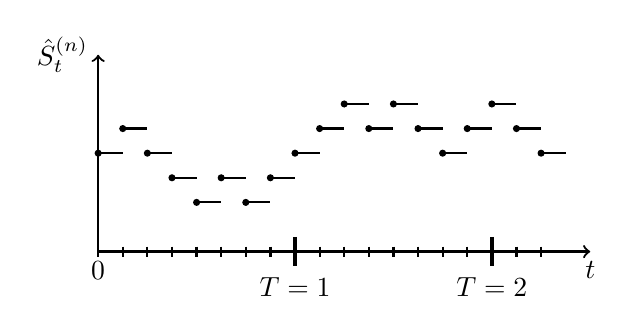
\begin{tikzpicture}[scale=1.25]
\draw[thick,->] (0,0) node[below] {$0$} 
  -- (5,0) node[below] {$t$};
\draw[thick,->] (0,0) -- (0,2) node[left] {$\hat S^{(n)}_t$};
\draw[thick] (0,1) --  (0.25,1);
\draw[thick] (0.25,1.25) -- (0.5,1.25);
\draw[thick] (0.5,1) -- (0.75,1);
\draw[thick] (0.75,0.75) -- (1,0.75);
\draw[thick] (1,0.5) -- (1.25,0.5);
\draw[thick] (1.25, 0.75) -- (1.5, 0.75);
\draw[thick] (1.5,0.5) -- (1.75,0.5);
\draw[thick] (1.75,0.75) -- (2,0.75);
\draw[thick] (2,1) -- (2.25,1);
\draw[thick] (2.25,1.25) -- (2.5,1.25);
\draw[thick] (2.5,1.5) -- (2.75,1.5);
\draw[thick] (2.75, 1.25) -- (3,1.25);
\draw[thick] (3,1.5) -- (3.25,1.5);
\draw[thick] (3.25,1.25) -- (3.5,1.25);
\draw[thick] (3.5,1) -- (3.75,1);
\draw[thick] (3.75,1.25) -- (4,1.25);
\draw[thick] (4,1.5) -- (4.25,1.5);
\draw[thick] (4.25,1.25) -- (4.5,1.25);
\draw[thick] (4.5,1) -- (4.75,1);
\filldraw (0,1) circle (0.03); 
\filldraw (0.25,1.25) circle (0.03);
\filldraw (0.5,1) circle (0.03);
\filldraw (0.75,0.75) circle (0.03);
\filldraw (1,0.5) circle (0.03);
\filldraw (1.25,0.75) circle (0.03);
\filldraw (1.5,0.5) circle (0.03);
\filldraw (1.75,0.75) circle (0.03);
\filldraw (2,1) circle (0.03);
\filldraw (2.25,1.25) circle (0.03);
\filldraw (2.5,1.5) circle (0.03);
\filldraw (2.75,1.25) circle (0.03);
\filldraw (3,1.5) circle (0.03);
\filldraw (3.25,1.25) circle (0.03);
\filldraw (3.5,1) circle (0.03);
\filldraw (3.75,1.25) circle (0.03);
\filldraw (4,1.5) circle (0.03);
\filldraw (4.25,1.25) circle (0.03);
\filldraw (4.5,1) circle (0.03);
\draw[very thick] (2,0.15)--(2,-0.15) node[below,black] {$T=1$};
\draw[very thick] (4,0.15)--(4,-0.15) node[below,black] {$T=2$};
\foreach \i in {0,0.25,0.5,0.75,1,1.25,1.5,1.75,2.25,2.5,2.75,3,3.25,3.5,3.75,4.25,4.5} 
\draw[thick] (\i,0.05)--(\i,-0.05);
\end{tikzpicture}
\centering
\caption{Качественный вид процесса $\hat S_t^{(n)}$.}
\label{crrl:fig}
\end{figure}

Далее под сходимостью случайных процессов по распределению будем понимать сходимость порождаемых ими мер на пространстве Скорохода.
Подробнее о сходимости случайных процессов, см., например, \cite{BulinskiShiryaev04}, гл.~V. 
О броуновском движении и геометрическом броуновском движении, которые упоминаются в предложении, см.~лекцию \ref{ch:processes}.

\begin{proposition}
Функции $\hat B^{(n)}$ сходятся равномерно по $t\in[0,T]$: $\hat B^{(n)}_t \rightrightarrows e^{rt}$ при $n\to\infty$.
Процессы $\hat S^{(n)}$ сходятся по распределению: $(\hat S_t^{(n)})_{t\in[0,T]} \xrightarrow{\text{d}} (\hat S_t)_{t\in[0,T]}$, где предельный процесс имеет вид $\hat S_t = S_0 \exp((r- \frac{\sigma^2}{2}) t + \sigma W_t)$ со стандартным броуновским движением $W$, и, таким образом, $\hat S$ является геометрическим броуновским движением.
\end{proposition}

Доказательство утверждения для $\hat B^{(n)}$ остается в качестве упражнения, а доказательство для $\hat S^{(n)}$ является следствием принципа инвариантности Донскера"--~Прохорова (см.~\cite{BulinskiShiryaev04}, гл.~V).


\section{Предел цен платежных обязательств}

\begin{proposition}
\label{crrl:p:convergence-2}
Пусть $f(s)$ является непрерывной неотрицательной функцией на $\R_+$, удовлетворяющей условию $f(s) \le c(1+s^p)$ для всех $s\ge 0$, где $c$ и $p$ "--- некоторые неотрицательные константы.
Обозначим за $V^n$ цену (в момент времени 0)  платежного обязательства с выплатой $f(S_{Tn}^{(n)})$, производимой в момент времени $Tn$ в модели с индексом $n$.
Тогда 
\begin{equation}
\label{crrl:limit}
V^n \to e^{-rT} \E f(S_T)\ \text{при}\ n\to\infty,
\end{equation}
где $S_T = S_0 \exp((r-\frac{\sigma^2}{2})T + \sigma W_T)$, а величина $W_T$ имеет нормальное распределение с нулевым средним и дисперсией $T$.
\end{proposition}

\begin{remark}
В правой части формулы \eqref{crrl:limit} стоит ничто иное, как цена платежного обязательства с функцией выплаты $f$ в модели \bs.
В частности, отсюда получается формулу \bs\ для цен европейских опционов колл и пут, если вычислить математическое ожидание.
\end{remark}

\begin{proof}[Доказательство предложения \ref{crrl:p:convergence-2}]
Заметим, что $V^n = \E^{Q^{(n)}} f(S_{Tn}^{(n)}) / B_{Tn}^{(n)}$. 
Как показано в предложении \ref{crrl:p:convergence-1}, имеем $B_{Tn}^{(n)} \to e^{rT}$, а также $S_{Tn}^{(n)} \xrightarrow{\text{d}} S_T$.
Тогда, если функция $f$ ограничена, то доказываемое утверждение следует из определения сходимости по распределению%
\footnote{Сходятся математические ожидания любой непрерывной ограниченной функции от рассматриваемой последовательности случайных величин (одно из эквивалентных определений сходимости по распределению).}.

Чтобы доказать утверждение для неограниченной функции $f$, нам потребуются следующие вспомогательные результаты.

\begin{definition}
Последовательность случайных величин $Y_n$ называется \emph{асимптотически равномерно интегрируемой}, если 
\[
\lim_{n\to\infty} \limsup_{m\to\infty} \E|Y_n| \I(|Y_n|>m) = 0.
\]
\end{definition}

\begin{lemma}[см.~\cite{VanDerVaart98}, теорема 2.20]
\label{crrl:l:aui}
Пусть $f(x)$ "--- непрерывная функция на $\R$, а последовательность случайных величин $X_n$ сходится к $X$ по распределению, причем последовательность $f(X_n)$ асимптотически равномерно интегрируема.
Тогда $\E f(X_n) \to \E f(X)$. 
\end{lemma}

Вернемся к доказательству предложения \ref{crrl:p:convergence-2}. Возьмем случайные величины $X_n$ с таким же распределением, как у $S_{Tn}^{(n)}$ по мере $\Q^{(n)}$, а $X$ с таким же распределением, как у $S_T$.
Покажем, что последовательность $Y_n = f(X_n)$ асимптотически равномерно интегрируема.  

Используя неравенства Коши"--~Буняковского и Чебышева, получаем оценку
\begin{equation}
\label{crrl:bound}
\E|Y_n| \I(|Y_n|>m) \le \sqrt{\E Y_n^2} \P(|Y_n| > m) \le \sqrt{\E Y_n^2} \frac{\E Y_n^2}{m^2} = \frac{(\E Y_n^2)^{\frac32}}{m^2}.
\end{equation}
Из условия $f(s) \le c(1+s^p)$ получаем
\[
\E Y_n^2 \le  c^2 + 2c\E X_n^p + c^2\E X_n^{2p}.
\]
Заметим, что $\E X_n^p = S_0^p ((1+u_n)^p q_n + (1-u_n)^p(1-q_n))^{Tn}$, и, используя формулу Тейлора можно непосредственно проверить, что $\E X_n^p$ имеет конечный предел при $n\to \infty$.
Следовательно, найдется константа $c_1$ такая, что $\E X_n^p < c_1$ при всех $n$.
Аналогично, $\E X_n^{2p} < c_2$ при всех $n$, и тогда $\E Y_n^2 \le c_3$ для некоторой константы $c_3$.
Отсюда и из оценки \eqref{crrl:bound} следует асимптотическая равномерная интегрируемость последовательности $Y_n$.
Применяя лемму \ref{crrl:l:aui}, доказательство теперь можно завершить так же, как в случае ограниченной функции $f$. 
\end{proof}

%!TEX root=finmath1.tex
\chapter{Доказательство первой фундаментальной теоремы}
\label{ch:ftap-proof}

Это дополнение содержит доказательство трудной импликации в первой фундаментальной теореме финансовой математики в дискретном времени (о том, что из безарбитражности следует существование эквивалентной мартингальной меры).


\section{План доказательства}

Для простоты мы будем рассматривать случай одного рискового актива и считать, что процентная ставка равна нулю ($B_t=1$ для всех $t$).
Доказательство в общем случае можно найти в оригинальной статье Даланга, Мортона и Виллинджера \cite{DalangMorton+90}; более короткое доказательство приведено в статье Кабанова и Стрикера \cite{KabanovStricker01}.

При наших предположениях докрываемую импликацию можно переформулировать в следующем абстрактном виде.

\begin{theorem}
\label{ftap-p:theorem}
Пусть на вероятностном пространстве $(\Omega,\F,\P)$ c фильтрацией $\FF=(\F_t)_{t=0}^T$ задана согласованная последовательность $S=(S_t)_{t=0}^T$ такая, что для любой предсказуемой последовательности $H=(H_t)_{t=1}^T$, удовлетворяющей неравенству $V_T^H := \sum_{t=1}^H H_t \Delta S_t \ge 0$ \as, выполнено $V_T^H = 0$ \as\ (гипотеза отсутствия арбитража NA). 

Тогда на $(\Omega,\F)$ существует вероятностная мера $\Q\sim\P$, относительно которой $S$ является мартингалом.
\end{theorem}

Доказательство будет состоять из трех шагов.
На первом шаге мы докажем замкнутость относительно сходимости \as\ множества $A$, состоящего из платежных обязательств, которые могут быть \emph{суперреплицированы}%
\footnote{Суперрепликация означает, что найдется торговая стратегия, стоимость портфеля которой в последний момент времени не меньше, чем выплата по заданному обязательству.} самофинансируемыми стратегиями, имеющими нулевую стоимость начального портфеля.  
Затем с помощью теоремы Крепа"--~Яна мы найдем вероятностную меру $\Q\sim\P$, разделяющую множества $A\cap L^1$ и $L_+^1$.
На третьем шаге будет показано, что $\Q$ является ЭММ.


\section{Вспомогательные результаты}

В этом разделе собраны вспомогательные результаты, которые нам потребуются.
Непосредственно для доказательства теоремы \ref{ftap-p:theorem} из них нужны только леммы \ref{ftap-p:l:kreps-yan}, \ref{ftap-p:l:subsequence}, \ref{ftap-p:l:strong-na}, а остальные используются для доказательства этих трех лемм.

\begin{lemma}[теорема Рисса; см.~\cite{Bogachev03}, теорема 2.2.5]
Пусть $X_n\to X$ в $L^1$ при $n\to\infty$.
Тогда найдется подпоследовательность $X_{n_k} \to X$ \as
\end{lemma}
\begin{remark}
Напомним, что $L^1$ "--- это пространство классов эквивалентности случайных величин с конечным математическим ожиданием и нормой $\|X\|_{L^1} = \E|X|$, относительно которой оно является банаховым пространством.
Под сходимостью $X_n\to X$ в $L^1$ понимают сходимость по норме, \te\ $\|X_n-X\|_{L^1} = \E|X_n-X| \to 0$.
В теории вероятностей ее также называют \emph{сходимостью в среднем}.
\end{remark}

\begin{corollary}
Пусть некоторое множество случайных величин $A$ замкнуто относительно сходимости \as\ (\te\ из сходимости $A\ni X_n \to X$ \as\ следует, что $X\in A$).
Тогда множество $A \cap L^1$ замкнуто в $L^1$.
\end{corollary}

\begin{proof}
Если $A \cap L^1 \ni X_n \to X$ в $L^1$, то по теореме Рисса найдется подпоследовательность $X_{n_k} \to X$ \as\
Тогда $X\in A$, и, значит, $X\in A\cap L^1$.
\end{proof}
  
\begin{definition}
Пусть $\{X_\lambda\}_{\lambda\in\Lambda}$ является семейством случайных величин, индексированных произвольным множеством $\Lambda$. \emph{Существенным супремумом} этого семейства называется случайная величина $S$ со значениями в $\R\cup\{+\infty\}$ такая, что $S \ge X_\lambda$ \as\ для любого $\lambda\in\Lambda$, и при этом для любой случайной величины $S'$ с таким же свойством выполнено неравенство $S'\ge S$ \as

Обозначение: $\esssup_{\lambda\in\Lambda} X_\lambda$.
\end{definition}

\begin{lemma}[см.~\cite{Shiryaev04}, гл.~VII, \S\,13.3]
У любого семейства случайных величин существует существенный супремум, единственный с точностью до равенства \as\ 
Более того, всегда можно выбрать такое счетное подсемейство $(X_{\lambda_n})_{n=1}^\infty$, что величина $S(\omega) = \sup_{n\ge1} X_{\lambda_n}(\omega)$ является существенным супремумом.
\end{lemma}

\begin{remark}
Нельзя просто определить $S(\omega) = \sup_{\lambda\in\Lambda} X_\lambda(\omega)$ для каждого $\omega$, так как функция $S(\omega)$ может оказаться неизмеримой, когда множество $\Lambda$ несчетно.  
\end{remark}

\begin{lemma}[теорема Хана"--~Банаха об отделимости; см.~\cite{KolmogorovFomin76}, гл.~IV, \S\,1.3, следствие 2]
Пусть $A$ "--- выпуклое множество в нормированном пространстве $L$, а некоторый ненулевой элемент $x\in L$ не лежит в $A$.
Тогда найдется непрерывный линейный функционал $p$ на $L$ такой, что $p(x) >0$ и $p(a)\le 0$ для любого $a\in A$.
\end{lemma}

\begin{lemma}[теорема Крепса"--~Яна]
\label{ftap-p:l:kreps-yan}
Пусть $A\subseteq L^1$ "--- выпуклое множество, причем $A\supseteq -L^1_+$ и $A\cap L^1_+ = \{0\}$, где $L_+^1$ "--- множество неотрицательных случайных величин с конечным математическим ожиданием на вероятностном пространстве $(\Omega,\F,\P)$.
Тогда найдется вероятностная мера $\Q\sim\P$ такая, что $\E^{\Q} X \le 0 $ для всех $X\in A$.
\end{lemma}

\begin{proof}
Пусть $L^\infty$ обозначает нормированное пространство классов эквивалентности ограниченных случайных величин с нормой $\|X\|_{L^\infty} = \inf\{c\ge 0 : |X| \le c\ \as\}$. Известно, что $L^\infty$ является банаховым пространством, причем оно двойственно к пространству $L^1$, \te\ любой непрерывный линейный функционал $p$ на $L^1$ можно отождествить с элементом $Z\in L^\infty$ по правилу $p(X) = \E(ZX)$.

Тогда по теореме Хана"--~Банаха для любого $X\in L^1_+\setminus\{0\}$ найдется случайная величина $Z_X\in L^\infty$ такая, что $\E Z_X X > 0$ и $\E Z_X X' \le 0$ для любого $X'\in A$.
Так как $A\supseteq - L^1_+$, то $Z_X\ge 0$.
Более того, можно считать, что $\|Z_X\|_{L^\infty} = 1$ (иначе поделим $Z_X$ на $\|Z_X\|_{L^\infty}$).

Положим $S = \esssup_{X\in L^1_+\setminus\{0\}} Z_X$.
Заметим, что $S \le 1$, так как $Z_X \le 1$.
Кроме того, $S>0$, так как иначе нельзя было бы отделить $X=\I(S=0)$ от $A$. 

Пусть $X_k\in L_+^1\setminus\{0\}$ является таким счетным семейством, что $S = \sup_k Z_{X_k}$.
Определим $Z = c \sum_{k=1}^\infty 2^{-k} Z_{X_k}$, где константа $c$ выбирается так, чтобы сделать $\E Z = 1$.
Заметим, что ряд для $Z$ сходится в $L^\infty$, причем $Z>0$ \as\ и $\E ZX' \le 0$ для всех $X'\in A$.
Тогда искомую меру можно задать в виде\footnote{Запись $d\Q = Z d\P$ означает, что $Z$ "--- это плотность Радона"--~Никодима $\Q$ относительно $\P$. Подробнее см.~раздел~\ref{itopr:girsanov} в лекции~\ref{ch:itopr}.} $d\Q = Z d\P$.
\end{proof}

\begin{lemma}[о сходящейся подпоследовательности]
\label{ftap-p:l:subsequence}
Предположим, что последовательность случайных величин $X_n$, $n\ge 0$, такова, что $\liminf_{n\to\infty} |X_n| < \infty$ \as\ 
Тогда найдется такая строго возрастающая случайная последовательность $\sigma_n$ со значениями в $\mathbb{Z}_+$, что последовательность $X_{\sigma_n}$ имеет предел \as\ при $n\to\infty$.
\end{lemma}

\begin{proof}
Положим $X = \liminf_{n\to\infty} |X_n|$.
Определим $\tau_0=0$, а для $n\ge 1$ положим
\[
\tau_n(\omega) 
  = \min\{k>\tau_{n-1}(\omega) : |X(\omega) - |X_k(\omega)|| < 1/n\}.
\]
Обозначим $\tilde X_n := X_{\tau_n}$.
Заметим, что $\sup_{n\ge 0} |\tilde X_n| < \infty$ \as, и, следовательно, $\tilde X := \liminf_{n\to\infty} \tilde X_n < \infty$.
Определим $\eta_0=0$ и
\[
\eta_n(\omega) = \inf\{k > \eta_{n-1}(\omega) 
  : |\tilde X(\omega) - \tilde X_k(\omega)| < 1/n\}.
\]
Тогда имеет место сходимость $\tilde X_{\eta_n} \to \tilde X$ \as, а, кроме того, $\tilde X_{\eta_n} = X_{\tau_{\eta_n}}$.
Следовательно, в качестве искомой последовательности можно взять $\sigma_n = \tau_{\eta_n}$.
\end{proof}

\begin{lemma}[об усиленном свойстве безарбитражности]
\label{ftap-p:l:strong-na}
Предположим, что на вероятностном пространстве $(\Omega,\F,\P)$ c фильтрацией $\FF=(\F_t)_{t=0}^T$ задана согласованная последовательность $S=(S_t)_{t=0}^T$, удовлетворяющая гипотезе NA в том виде, как она сформулирована в теореме \ref{ftap-p:theorem}.

Пусть $V_T^H := \sum_{t=1}^T H_t\Delta S_t \ge 0$ для некоторой предсказуемой последовательности $H$. 
Тогда для этой последовательности $V_t^H := \sum_{u=1}^t H_u\Delta S_u = 0$ при всех $t=1,\dots,T$.
\end{lemma}

\begin{proof}
Сначала докажем, что $V_t^H\ge 0$ для всех $t$.
Предположим противное и возьмем первое $t$ для которого $\P(V_t^H<0)>0$. 
Положим $\tilde H_u = 0$ при $u\le t$ и $\tilde H_u = H_u\I(V^H_t<0)$ при $u> t$.
Тогда имеем
\[
V_T^{\tilde H} = \sum_{u=t+1}^T \tilde H_u \Delta S_u 
= \I(V^H_t<0) \sum_{u=t+1}^T H_u\Delta S_u = -\I(V^H_t<0) V_t^H.
\]
Следовательно, $V_T^{\tilde H} \ge 0$ и $\P(V_T^{\tilde H}>0)>0$, что противоречит гипотезе NA.

Теперь предположим, что $\P(V_t^H>0)>0$ для некоторого $t$.
Положим $\tilde H_u = H_t$ при $u\le t$ и $\tilde H_u = 0$ при $u> t$.
Тогда $V_T^{\tilde H} = \sum_{u=1}^t H_u\Delta S_u = V_t^H$.
Снова получаем $V_T^{\tilde H} \ge 0$ и $\P(V_T^{\tilde H}>0)>0$, что противоречит гипотезе NA.
\end{proof}


\section{Доказательство теоремы}

\textit{Шаг 1.} Определим множество платежных обязательств, суперреплицируемых самофинансируемыми стратегиями с нулевой стоимостью начального портфеля:
\begin{multline*}
A = \biggl\{X : X \le \sum_{t=1}^T H_t\Delta S_t,
  \ \text{где $H$ предсказуема}\biggr\} \\
= \biggl\{\sum_{t=1}^T H_t\Delta S_t - \gamma : 
  \text{$H$ предсказуема, $\gamma\ge 0$ "--- $\F_T$-измерима}\biggr\}.
\end{multline*}
Покажем, что $A$ замкнуто относительно сходимости \as\ 

Пусть $X^n = \sum_{t=1}^T H_t^n \Delta S_t - \gamma^n \to X$ \as\ 
Нужно показать, что $X\in A$.
Докажем это индукцией по $T$.
Для $T=0$ утверждение очевидно.
Предположим, что оно доказано для $T-1$ и $\sum_{t=1}^T H_t^n\Delta S_t - \gamma^n \to X$ \as\ 
Положим
\[
\Omega_1 = \left\{\omega : \liminf_{n\to\infty} |H_1^n(\omega)| < \infty\right\}.
\]
По лемме о сходящейся подпоследовательности, найдутся $\F_0$-измеримые величины $\sigma_n$ такие, что предел $H_1:=\lim\limits_{n\to\infty }H_1^{\sigma_n} \I_{\Omega_1}$ существует и конечен.

Пусть $\Omega_2 = \Omega\setminus\Omega_1$.
Покажем, что $\Delta S_1 = 0$ \as\ на $\Omega_2$.
Положим $G_t^n = H_t^n/|H_1^n|$ и $f^n = \gamma^n/|H_1^n|$.
Тогда
\[
\lim_{n\to\infty}\biggl(\sum_{t=1}^T G_t^n\Delta S_t - f^n\biggr) 
= \lim_{n\to\infty} \frac{X}{|H_1^n|} =  0\ \text{на $\Omega_2$}.
\]
По лемме о сходящейся подпоследовательности найдутся величины $\tau_n$ такие, что $G_1'^n := G_1^{\tau_n}\I_{\Omega_2} \to G_1'$.
Заметим, что $G_1'$ принимает значения $\pm1$ на $\Omega_2$. 
Пусть $f'^n = f^{\tau_n}$.
Тогда
\[
\sum_{t=2}^T G_t'^n \Delta S_t - f'^n \to - G'_1 \Delta S_1\ \text{на $\Omega_2$}.
\]
По предположению индукции существуют $\tilde G_t'$, $t=2,\dots,T$, и $\tilde f'\ge 0$ такие, что 
\[
\sum_{t=2}^T \tilde G_t' \Delta S_t - \tilde f' = -  G'_1 \Delta S_1.
\]
Пусть $\tilde G_1' = G_1'$.
Тогда $\sum_{t=1}^T \tilde G_t' \Delta S_t = \tilde f'$.
В силу усиленной гипотезы безарбитражности, имеем $\tilde G_1'\Delta S_1 = 0$.
Так как $\tilde G_1'\in\{-1,1\}$ на $\Omega_2$, то $\Delta S_1 = 0$ \as\ на $\Omega_2$. 

Найдем теперь такие $H$ и $\gamma$, что $X=\sum_{t=1}^T H_t\Delta S_t - \gamma$.
Определим $\tilde H_t^n = H^{\sigma_n}_t$, $\tilde \gamma^n = \gamma^{\sigma_n}$.
Так как $\tilde H_1^n\Delta S_1 \to H_1\Delta S_1$ и $\sum_{t=1}^T \tilde H_t^n \Delta S_1 - \tilde \gamma^n \to X$,
то имеем
\[
\sum_{t=2}^T \tilde H_t^n \Delta S_1 - \tilde \gamma^n \to X - H_1 \Delta S_1.
\]
По предположению индукции существуют $H_t$, $t=2,\dots,T$, и $\gamma\ge 0$ такие, что
\[
\sum_{t=2}^T H_t \Delta S_1 - \gamma = X - H_1 \Delta S_1.
\]
Отсюда уже легко следует доказываемое утверждение.

\medskip
\emph{Шаг 2.}
Далее без ограничения общности будем считать, что $\E|S_t| < \infty$ для всех $t=1,\dots,T$.
Если это не так, что можно перейти к мере $\P' \sim \P$ с плотностью
\[
\frac{d\P'}{d\P} = c e^{-\sum\limits_{t=1}^T |S_t|},
\]
где $c$ "--- нормализующая константа.
Тогда $\E^{\P'} |S_t| < \infty$ и достаточно заметить, что замена меры на эквивалентную сохраняет свойство замкнутости относительно сходимости \as, а также справедливость гипотезы NA.

Обозначим $A^1 = A \cap L^1$.
Имеем $A^1\supset -L^1_+$ по определению $A$.
Кроме того, $A^1\cap L^1_+ = \{0\}$ в силу гипотезы NA.
Тогда по теореме Крепса"--~Яна найдется мера $\Q\sim\P$, для которой
\[
\E^{\Q} X \le 0\ \text{для всех}\ X\in A^1.
\]

\medskip
\textit{Шаг 3.}
Проверим, что мера $\Q$ является ЭММ.
Нужно показать, что для всех $t=0,\dots,T-1$ выполнено равенство $\E^{\Q} (S_{t+1}\mid \F_t) = S_t$.
Предположим, от противного, что $\Q(B) > 0$ для некоторого множества $B = \{\omega : \E (S_{u+1}\mid \F_u)(\omega) > S_u(\omega)\}$.

Рассмотрим последовательность $H_t$, в которой $H_{u+1} = \I_B$ и $H_t = 0$ для всех $t\neq u+1$.
Пусть $X = \sum_{t=1}^T H_t\Delta S_t$.
Тогда $X\in A^1$, так как $H$ ограничена и $\E^{\Q} |S_t| < \infty$.
Следовательно, $\E^{\Q} X = \E^Q \I_B (S_{t+1}-S_t) > 0$ "--- противоречие с конструкцией $\Q$.

Таким образом, $\Q(B) = 0$, и поэтому $\E (S_{t+1} \mid \F_t) \ge S_t$ для всех $t$.
Неравенство в другую сторону доказывается аналогично.
Следовательно, $\Q$ является ЭММ.

%!TEX root=finmath1.tex
\chapter{Модель Башелье}
\label{ch:bachelier}

Модель Башелье "--- это первая модель финансового рынка (1900 г.)%
\footnote{Модель была предложена в диссертации Л.~Башелье \cite{Bachelier00}.
Долгое время, до 1960-х гг., большинству экономистов она была не известна, хотя в классических работах по теории вероятностей, в т.\,ч.~в работах А.\,Н.~Колмогорова, результаты Башелье упоминаются.}.
Говоря современным языком, процесс цены рискового актива в ней задается броуновским движением со сносом.
В этом дополнении дается описание модели Башелье и доказывается формула для цены европейских опционов колл и пут, аналогичная формуле \bs.

\section{Описание модели}
Структура модели во многом схожа с моделью \bs, поэтому мы опустим подробные пояснения.

Будем считать заданным некоторое фильтрованное вероятностное пространство $(\Omega,\F,\FF,\P)$, в котором фильтрация $\FF=(\F_t)_{t\in[0,T]}$ порождена броуновским движением $W=(W_t)_{t\in[0,T]}$ и пополнена.

В модели имеются два актива.
Безрисковый актив имеет цену $B_t\equiv 1$, \te\ процентная ставка равна 0, а цена рискового актива задается процессом
\[
S_t = s_0 + \mu t + \sigma W_t.
\]
Отметим, что цена рискового актива может стать отрицательной,
это один из недостатков модели%
\footnote{Однако отметим, что возможность модели Башелье учитывать отрицательные цены оказалась полезной в апреле 2020 г., когда цены поставочных фьючерсов на нефть стали отрицательными из-за отсутствия свободных емкостей для принятия поставок.
В частности, Чикагская товарная биржа на некоторое время сменила используемую модель для расчета цен опционов на фьючерсы с модели Блэка на модель Башелье.}.
% https://www.cmegroup.com/notices/clearing/2020/04/Chadv20-171.html

Торговой стратегией будем называть процесс $\pi_t=(G_t,H_t)$ с компонентами $G\in \PP_T^1$ и $H\in\PP_T^2$.
Стоимость портфеля стратегии $\pi$ выражается процессом
\[
V_t^\pi = G_t + H_tS_t.
\]
Стратегия называется самофинансируемой, если
\[
d V_t^\pi = H_t dS_t.
\]

Следующее предложение и следствие из него доказываются так же, как в модели \bs.

\begin{proposition}
В модели Башелье существует единственная вероятностная мера $\Q\sim\P$ такая, что процесс процесс $S$ является мартингалом относительно $\Q$.
Более того, справедливо представление $S_t = s_0 + \sigma W_t^\Q$, где $W_t^\Q = W_t - \mu t/\sigma$ "--- броуновское движение относительно $\Q$.

Стоимость портфеля любой самофинансируемой стратегии $V_t^\pi$ является локальным мартингалом относительно $\Q$, а если стратегия допустима в том смысле, что $H\in \L^2_T(\Q)$, то $V_T^\pi$ является квадратично интегрируемым мартингалом.
\end{proposition}

\begin{corollary}
В модели Башелье нет арбитража.
\end{corollary}

\section{Цены платежных обязательств}
Будем отождествлять платежные обязательства европейского типа с $\F_T$-измеримыми случайными величинами $X$ такими, что $\E^\Q X^2 < \infty$.  

Следующее предложение вытекает из теоремы о мартингальном представлении и того факта, что стоимость любой допустимой самофинансируемой стратегии является мартингалом относительно ЭММ.

\begin{proposition}
В модели Башелье любое платежное обязательство  является реплицируемым, причем реплицирующая стратегия единственна.
Цена репликации (стоимость реплицирующего портфеля) равна
\[
V_t^X = \E^\Q (X \mid \F_t).
\]
\end{proposition}

Если платежное обязательство зависит только от значения цены в последний момент времени, $X=f(S_T)$, то его цену можно найти вычислением условного математического ожидания, пользуясь тем, броуновскогое движение "--- это марковский процесс с известной переходной плотностью. А именно, $V_t^X = V(t,S_t)$ с функцией
\[
V(t,s) = \int_\R f(s + \sigma x\sqrt{T-t}) \phi(x) dx.
\]

\begin{corollary}[формула Башелье]
Для цен европейских опционов колл и пут в модели Башелье справедлива формула
\[
\begin{aligned}
&\VC(t,s) = (s-K)\Phi(d) + \sigma \sqrt{T-t}\phi(d),\\
&\VP(t,s) = (K-s)\Phi(-d) + \sigma\sqrt{T-t}\phi(d),
\end{aligned}
\]
где $d = (s-K) /(\sigma\sqrt{T-t})$.
\end{corollary}

% \begin{corollary}
% Пусть $x=f(S_T)$, где $|f(s)|  \le  ce^{m|s|}$ для некоторых констант $c,m$.
% Тогда цена репликации платежного обязательства $X$ представима в виде $V_t^X = V(t,S_t)$ с функцией
% \[
% V(t,s) = \int_\R f(s + \sigma x\sqrt{T-t}) \phi(x) dx
% \]
% и удовлетворяет уравнению с частными производными
% \[
% \left\{\begin{aligned}
% &V'_t(t,s) + \frac{\sigma^2}{2} V''_{ss}(t,s) = 0, \qquad t\in[0,T),\ s\in \R,\\
% &V(T,s) = f(s), \qquad s\in\R,
% \end{aligned}
% \right.
% \]
% а компонента $H$ реплицирующей стратегии задается формулой $H_t = V'_s(t,S_t)$.
% \end{corollary}

%!TEX root=finmath1.tex
\chapter{Модель Блэка для рынка фьючерсов}
\label{ch:black}

Здесь более подробно излагается модель Блэка для рынка фьючерсов (она кратко упоминалась в замечании \ref{bs2:r:black} в лекции \ref{ch:bs2}), в которой моделируется непосредственно цена фьючерса, без введения в рассмотрение базового актива.

\section{Описание модели}
В модели имеются два актива "--- безрисковый актив с детерминированной процентной ставкой и рисковый актив, являющийся фьючерсом с моментом экспирации $T'\ge T$.
Клиринг происходит <<непрерывно>> во времени.

Основные объекты и понятия, вводимые далее, будут такими же, как в модели \bs, но определение стоимости портфеля будет иметь другой вид: оно будет учитывать, что открыть и закрыть позицию по фьючерсу в любой момент можно без издержек (см.~пояснение в разделе \ref{fut:ss:assets} лекции \ref{ch:futures-discrete}).

Итак, пусть задано фильтрованное вероятностное пространство $(\Omega,\F,\FF,\P)$ с фильтрацией $\FF=(\F_t)_{t\in[0,T]}$, которая порождена броуновским движением $W=(W_t)_{t\in[0,T]}$ и пополнена.

Цены безрискового актива и фьючерса имеют вид
\[
d B_t = r(t) B_t dt,\quad B_0=1, \qquad d F_t = \mu F_t dt + \sigma F_t dW_t, \quad F_0 = f_0>0.
\]
Функция $r(t)$ считается измеримой и ограниченной.

Торговой стратегией называется процесс $\pi_t=(G_t,H_t)$, где $G\in \PP_T^1$, $H\in\PP_T^2$.
Стоимость портфеля стратегии $\pi$ по определению равна
\begin{equation}
\label{bl:portfolio-value}
V_t^\pi = G_tB_t
\end{equation}
(заметим, что стоимость фьючерсной позиции равна нулю). 
Дисконтированная стоимость портфеля $\tilde V_t^\pi = V_t^\pi/B_t$ совпадает с процессом $G_t$.

Стратегия называется самофинансируемой, если
\begin{equation}
\label{bl:sf}
d V_t^\pi = G_t d B_t + H_t dF_t.
\end{equation}

\begin{proposition}
В модели Блэка существует единственная вероятностная мера $\Q\sim\P$ такая, что процесс $F$ является мартингалом относительно $\Q$:
\[
d F_t = \sigma F_t d W_t^{\Q},
\] 
где $W_t^Q$ "--- броуновское движение относительно $\Q$. 

Кроме того, процесс $G$ любой самофинансируемой стратегии (и, следовательно, дисконтированная стоимость ее портфеля) является локальным мартингалом относительно $\Q$.
При этом $G$ является квадратично интегрируемым мартингалом, если $HF\in \L^2_T(\Q)$.
\end{proposition}

\begin{proof}
Кратко перечислим лишь основные шаги доказательства, так как оно идейно повторяет доказательства аналогичных результатов в модели \bs.

Мера $\Q$ строится по теореме Гирсанова.
Если $\pi$ "--- самофинансируемая стратегия, то, применяя формулу Ито к \eqref{bl:sf}, показывается, что дисконтированная стоимость $\tilde V_t^\pi = V_t^\pi/B_t\;(=G_t)$ удовлетворяет уравнению
\[
d\tilde V_t^\pi = \frac{H_t}{B_t} dF_t = \frac{\sigma H_t F_t}{B_t}dW_t^{\Q},
\]
откуда следует, что это локальный мартингал.
Если выполнено условие $HF \in \L^2_T(\Q)$, то он квадратично интегрируем по свойству интеграла Ито.
\end{proof}
\begin{remark}
Полученная цена фьючерса имеет точно такой же вид относительно ЭММ, как в разделе \ref{bs2:ss:futures} лекции \ref{ch:bs2}.
Зачем же нам тогда понадобилось рассматривать новую модель?

Отличие между моделью там и здесь состоит в том, что теперь мы не предполагаем, что на рынке торгуется сам базовый актив, с которым связан фьючерс, и, как следствие, не требуем, чтобы дисконтированная цена базового актива являлась мартингалом относительно ЭММ. 
%
% В качестве примера можно привести фьючерсы на индекс волатильности VIX\footnote{Индекс VIX вычисляется по подразумеваемой волатильности опционов на индекс S\&P\,500, исполняющихся через месяц, и показывает <<насколько волатилен>> сейчас рынок.
% Более подробно мы его коснемся в курсе <<Модели стохастической волатильности>>.}. 
% Этот индекс не является торгуемым инструментом, однако торгуются фьючерсы на VIX.
% В частности, в безарбитражной модели процесс значения индекса VIX (он сам или дисконтированный) не обязан быть мартингалом, а цена фьючерса обязана.
\end{remark}


\section{Цены платежных обязательств. Формула Блэка}

\subsection{Премиальные платежные обязательства}
Будем отождествлять платежные обязательства с $\F_T$"=измеримыми случайными величинами $X$ такими, что $\E^\Q X^2 < \infty$.
В этом разделе мы рассмотрим премиальные платежные обязательства, по которым, как обычно, покупатель платит продавцу премию (цену обязательства) в момент $t$, а получает выплату $X$ в момент $T$.
В следующем разделе будут рассмотрены маржируемые контракты.

\begin{proposition}
В модели Блэка любое квадратично интегрируемое платежное обязательство $X$ является реплицируемым, причем реплицирующая стратегия единственна.
Цена репликации (стоимость портфеля реплицирующей стратегии) равна
\[
V_t^X = B(t,T)\E^\Q (X \mid \F_t),
\]
где $B(t,T) = e^{-\int_t^T r(s)ds}$ "--- цена бескупонной облигации.
\end{proposition}

В качестве частного случая рассмотрим европейские опционы колл и пут на фьючерс "--- это контракты, дающие право покупателю в будущий момент времени $T$ открыть длинную (опцион колл) или короткую (опцион пут) фьючерсную позицию по фиксированной цене $K$.
Считается, что экспирация фьючерса происходит не раньше экспирации опционов.
Эти опционы можно отождествить с выплатами, производимыми в момент $T$ и равными
\[
X^\text{call} = (F_T-K)^+, \qquad X^\text{put} = (K-F_T)^+,
\]
где $F_T$ "--- цена фьючерса с временем экспирации $T'\ge T$. 

\begin{corollary}[формула Блэка]
\label{bl:c:black-formula}
Цены опционов на фьючерс в модели Блэка имеют вид $V_t=V(t,F_t)$, где
\[
\begin{aligned}
&\VC(t,f) = B(t,T) (f\Phi(d_1) - K\Phi(d_2)), \\
&\VP(t,s) = B(t,T) (K\Phi(-d_2) - f\Phi(-d_1)),\\
&d_1 = \frac{1}{\sigma\sqrt{T-t}} \left(\ln\frac{f}{K} + \frac{\sigma^2}{2}(T-t)\right), \quad
d_2 = d_1 - \sigma\sqrt{T-t}.
\end{aligned}
\]
\end{corollary}

Отметим, что полученная формула имеет такой же вид, как формула Блэка из лекции \ref{ch:bs2}, но там $f$ выражает $T$-форвардную цену базового актива, а здесь "--- цену фьючерса (они совпадают в модели \bs, если $T=T'$).
Величина $T'$ не входит в формулу.


\subsection{Маржируемые контракты}

Для маржируемого контракта в модели Блэка величина $X$ задает расчетную цену в момент $T$.
Ценой репликации контракта называется такой процесс $V^X = (V_t^X)_{t\in[0,T]}$, что существует стратегия $\pi_t=(G_t,H_t)$ с компонентами $G\equiv 0$ и $H\in \PP_T^2$ (не являющаяся в общем случае самофинансируемой), удовлетворяющая условию
\[
d V_t^X = H_t d F_t.
\]
Это равенство означает, что изменение стоимости портфеля стратегии в точности равно вариационной марже.
Поясним, что условие $G_t\equiv 0$ возникает по той причине, что стоимость портфеля реплицирующей стратегии должна быть нулевой (так как позицию по маржируемому контракту можно открывать и закрывать ьез издержек), а стоимость портфеля определяется формулой \eqref{bl:portfolio-value}.
Таким образом, реплицирующая стратегия торгует только фьючерсом.

\begin{proposition}
В модели Блэка реплицирующая стратегия любого маржируемого контракта $X$ единственна $($в классе стратегий с $HF\in \L^2_T(\Q)$$)$, а цена репликации равна
\[
V_t^X = \E^\Q (X \mid \F_t).
\]
\end{proposition}

\begin{corollary}[формула Блэка для маржируемых опционов]
Цены маржируемых опционов колл и пут $($\te\ маржируемых контрактов с расчетными ценами $X^\text{call} = (F_T - K)^+$ и $X^\text{put} = (K-S_T)^+$$)$ имеют вид $V_t = V(t,F_t)$, где
\[
\VC(t,f) = f\Phi(d_1) - K\Phi(d_2), \qquad
\VP(t,s) = K\Phi(-d_2) - f\Phi(-d_1),
\]
а величина $d$ такая, же как в следствии \ref{bl:c:black-formula}.
\end{corollary}

%%!TEX root=finmath1.tex
\chapter{Фьючерсы и другие маржируемые контракты}
\label{ch:futures-discrete}
\chaptertoc

Фьючерс "--- это контракт на покупку/продажу базового актива в будущем, торгуемый на организованной бирже.
Исполнение фьючерса гарантируется специальным механизмом ежедневного перечислением вариационной маржи.
В этой лекции мы расширим модель рынка из лекции \ref{ch:general} и покажем, как включить в нее фьючерсы и другие маржируемые контракты, а также вычислим их безарбитражные цены.


\section{Механика торговли фьючерсами}
Для лучшего понимая математичкой теории, излагаемой в следующих разделах, мы сначала опишем как технически осуществляется торговля фьючерсами.
Приводимые рассуждения можно легко обобщить на другие контракты с механизмом перечисления вариационной маржи, о чем будет сказано в замечании \ref{fut:r:mtm-contract} в конце этого раздела.

Фьючерс можно представлять себе как контракт на поставку определенного актива в будущем. 
Фьючерс характеризуется базовым активом (акция, индекс, товар и \tp), датой экспирации, типом расчетов (расчетный или поставочный) и объемом лота (количество единиц базового актива в одном контракте).
По одному базовому активу одновременно в обращении находятся несколько фьючерсов с разными датами экспирации.
Наиболее далекие экспирации могут отстоять от текущего момента времени на несколько лет.
По расчетным фьючерсам все расчеты между покупателями и продавцами происходят в денежной форме; по поставочным фьючерсам, помимо промежуточных денежных расчетов, продавцы обязаны выполнить передачу базового актива покупателю, а покупатели обязаны заплатить соответствующую стоимость.

Фьючерсы торгуются на организованных биржах, и в каждый момент времени до даты экспирации имеется биржевая цена фьючерса, которая получается в результате взаимодействия покупателей и продавцов%
\footnote{Торги на современных биржах проходят в электронном режиме и по каждому инструменту доступна не какая-то одна цена, а список заявок на покупку и продажу (биржевой <<стакан>>, order book). 
Когда мы говорим о цене инструмента, то имеем ввиду, например, среднюю цену между лучшими ценами заявок на покупку и продажу.
Для дальнейших рассуждений такие детали несущественны; можно предполагать, что в каждый момент времени  цена однозначно определена.}.
Однако в отличие, скажем, от акций, когда покупатель должен заплатить продавцу текущую цену акции при ее покупке, или в отличие от форвардных контрактов, когда расчеты осуществляются только в последний момент времени, расчеты по фьючерсам проходят по-другому.

Сделка по фьючерсу состоит в том, что одна сторона (покупатель) открывает <<длинную>> позицию по текущей цене (покупает фьючерс), а другая сторона (продавец) "--- <<короткую>> позицию (продает фьючерс).
В момент следующего \emph{клиринга} покупатель фьючерса получает на свой счет денежную выплату, называемую \emph{вариационной маржой}, которая равна разнице между \emph{расчетной ценой} фьючерса на момент клиринга и ценой, по которой он открыл позицию.
Если эта величина отрицательна, то вариационная маржа списывается со счета покупателя.
Продавец получает на свой счет вариационную маржу, равную разнице между ценой фьючерса при открытии позиции и расчетной ценой на момент клиринга (вариационная маржа покупателя со знаком минус).
Клиринг происходит ежедневно или несколько раз в день (дневной и вечерний) и продолжается несколько минут; торги в это время приостанавливаются.
Расчетная цена определяется путем усреднения лучших заявок на покупку и продажу за небольшой промежуток времени до начала клиринга.

В каждый следующий клиринг покупатель, если он не закроет свою позицию, получает вариационную маржу, равную разнице расчетных цен текущего и предыдущего клиринга.
Если покупатель закрывает позицию, то в клиринг он получает разницу между ценой фьючерса на момент закрытия позиции и расчетной ценой предыдущего клиринга.
Под закрытием длинной позиции понимается открытие короткой позиции (продажа фьючерса).
Если покупатель открывает и закрывает длинную позицию по фьючерсу в промежуток времени между двумя клирингами, то он получают разницу между ценами в моменты закрытия и открытия позиции. 
Для продавца фьючерса все аналогично.

В день экспирации правила расчета такие же, как и в промежуточные дни, за исключением того, что расчетная цена фьючерса в последний клиринг полагается равной текущей цене базового актива, умноженной на размер лота.
Это как раз и выражает то обстоятельство, что фьючерс является контрактом на поставку базового актива в момент экспирации, и привязывает цену фьючерса к цене базового актива.
Подчеркнем, что до момента экспирации цена фьючерса устанавливается исключительно рыночными механизмами (спросом и предложением), однако мы покажем, что существует конкретное теоретическое соотношение между справедливой ценой фьючерса и ценой базового актива. 

Если фьючерс поставочный, то дополнительно после экспирации у покупателя фьючерса возникает обязательство купить базовый актив в объеме, равном размеру лота, по расчетной цене последнего клиринга; у продавца же возникает обязательство продать базовый актив.

\begin{example}
Рис.~\ref{fut:fig}  иллюстрирует расчеты по фьючерсу.
На этом рисунке фьючерс экспирируется в момент $t=4$ (единица времени здесь соответствует одному окну между клирингами).
Объема лота равен 1.
В момент времени $t_1\in (1,2)$ покупатель открывает длинную позицию.
В моменты 2 и 3 он получает положительную вариационную маржу $M_2$ и $M_3$ в связи с тем, что цена фьючерса выросла.
В момент времени $t_2 \in (3,4)$ покупатель закрывает длинную позицию по цене ниже, чем предыдущая расчетная цена, что приводит к списанию вариационной маржи $M_4$ в момент 4.
Так как в момент 4 фьючерс экспирируется, то его цена в этот момент совпадает с ценой базового актива.
\end{example}

\begin{figure}[h]
\centering
\begin{tikzpicture}[xscale=2.2,yscale=13]
\draw[very thick,dotted] 
  (0.00, 1.00) node[left] {\footnotesize $S_0$} --
  (0.04, 1.01)--(0.08, 1.02)--(0.12, 1.02)--(0.16, 1.02)--
  (0.20, 1.02)--(0.24, 1.02)--(0.28, 1.02)--(0.32, 1.03)--(0.36, 1.02)--
  (0.40, 1.03)--(0.44, 1.02)--(0.48, 1.02)--(0.52, 1.04)--(0.56, 1.03)--
  (0.60, 1.03)--(0.64, 1.04)--(0.68, 1.05)--(0.72, 1.04)--(0.76, 1.03)--
  (0.80, 1.04)--(0.84, 1.05)--(0.88, 1.06)--(0.92, 1.06)--(0.96, 1.05)--
  (1.00, 1.04)--(1.04, 1.05)--(1.08, 1.05)--(1.12, 1.05)--(1.16, 1.05)--
  (1.20, 1.04)--(1.24, 1.03)--(1.28, 1.03)--(1.32, 1.02)--(1.36, 1.03)--
  (1.40, 1.03)--(1.44, 1.04)--(1.48, 1.03)--(1.52, 1.05)--(1.56, 1.05)--
  (1.60, 1.04)--(1.64, 1.05)--(1.68, 1.05)--(1.72, 1.06)--(1.76, 1.06)--
  (1.80, 1.06)--(1.84, 1.07)--(1.88, 1.09)--(1.92, 1.10)--(1.96, 1.10)--
  (2.00, 1.11)--(2.04, 1.11)--(2.08, 1.11)--(2.12, 1.12)--(2.16, 1.12)--
  (2.20, 1.14)--(2.24, 1.14)--(2.28, 1.13)--(2.32, 1.14)--(2.36, 1.14)--
  (2.40, 1.15)--(2.44, 1.15)--(2.48, 1.17)--(2.52, 1.18)--(2.56, 1.21)--
  (2.60, 1.21)--(2.64, 1.20)--(2.68, 1.17)--(2.72, 1.18)--(2.76, 1.18)--
  (2.80, 1.19)--(2.84, 1.19)--(2.88, 1.22)--(2.92, 1.23)--(2.96, 1.22)--
  (3.00, 1.22)--(3.04, 1.22)--(3.08, 1.21)--(3.12, 1.22)--(3.16, 1.23)--
  (3.20, 1.21)--(3.24, 1.22)--(3.28, 1.23)--(3.32, 1.24)--(3.36, 1.22)--
  (3.40, 1.21)--(3.44, 1.21)--(3.48, 1.22)--(3.52, 1.24)--(3.56, 1.24)--
  (3.60, 1.25)--(3.64, 1.24)--(3.68, 1.24)--(3.72, 1.25)--(3.76, 1.24)--
  (3.80, 1.23)--(3.84, 1.25)--(3.88, 1.25)--(3.92, 1.23)--(3.96, 1.22)--
  (4.00, 1.21);

\draw[thick] 
  (0.00, 1.11) node[left] {\footnotesize $F_0$} --
  (0.04, 1.11)--(0.08, 1.12)--(0.12, 1.12)--(0.16, 1.13)--
  (0.20, 1.12)--(0.24, 1.12)--(0.28, 1.12)--(0.32, 1.13)--(0.36, 1.12)--
  (0.40, 1.13)--(0.44, 1.11)--(0.48, 1.12)--(0.52, 1.13)--(0.56, 1.13)--
  (0.60, 1.12)--(0.64, 1.13)--(0.68, 1.14)--(0.72, 1.13)--(0.76, 1.12)--
  (0.80, 1.13)--(0.84, 1.14)--(0.88, 1.15)--(0.92, 1.14)--(0.96, 1.14)--
  (1.00, 1.12)--(1.04, 1.13)--(1.08, 1.13)--(1.12, 1.13)--(1.16, 1.13)--
  (1.20, 1.11)--(1.24, 1.11)--(1.28, 1.10)--(1.32, 1.09)--(1.36, 1.11)--
  (1.40, 1.10)--(1.44, 1.11)--(1.48, 1.10)--(1.52, 1.11)--(1.56, 1.11)--
  (1.60, 1.10)--(1.64, 1.12)--(1.68, 1.12)--(1.72, 1.12)--(1.76, 1.13)--
  (1.80, 1.12)--(1.84, 1.13)--(1.88, 1.15)--(1.92, 1.16)--(1.96, 1.17)--
  (2.00, 1.17)--(2.04, 1.17)--(2.08, 1.18)--(2.12, 1.18)--(2.16, 1.18)--
  (2.20, 1.19)--(2.24, 1.19)--(2.28, 1.18)--(2.32, 1.19)--(2.36, 1.19)--
  (2.40, 1.19)--(2.44, 1.20)--(2.48, 1.21)--(2.52, 1.23)--(2.56, 1.25)--
  (2.60, 1.25)--(2.64, 1.24)--(2.68, 1.21)--(2.72, 1.22)--(2.76, 1.22)--
  (2.80, 1.23)--(2.84, 1.23)--(2.88, 1.26)--(2.92, 1.26)--(2.96, 1.25)--
  (3.00, 1.26)--(3.04, 1.25)--(3.08, 1.24)--(3.12, 1.25)--(3.16, 1.25)--
  (3.20, 1.24)--(3.24, 1.25)--(3.28, 1.25)--(3.32, 1.26)--(3.36, 1.24)--
  (3.40, 1.23)--(3.44, 1.23)--(3.48, 1.24)--(3.52, 1.25)--(3.56, 1.25)--
  (3.60, 1.26)--(3.64, 1.25)--(3.68, 1.25)--(3.72, 1.26)--(3.76, 1.25)--
  (3.80, 1.24)--(3.84, 1.26)--(3.88, 1.26)--(3.92, 1.24)--(3.96, 1.225)--
  (4.00, 1.21);

\draw[->] (0,0.95)--(4.5,0.95) node[below] {\footnotesize $t$};
\draw[->] (0,0.95)--(0,1.3) node[left] {\footnotesize Цена};

\foreach \i in {0,1,2,3,4} {
  \draw (\i,0.955)--(\i,0.945) node[below] {\footnotesize \i};
}

\filldraw (1.32, 1.09) ellipse (0.03 and 0.005);
\filldraw (2, 1.17) ellipse (0.03 and 0.005);
\filldraw (3, 1.26) ellipse (0.03 and 0.005);
\filldraw (3.4, 1.23) ellipse (0.03 and 0.005);

\draw[dotted] (0,1.09) -- (4.2,1.09);
\draw[dotted] (0,1.17) -- (4.2,1.17);
\draw[dotted] (0,1.26) -- (4.6,1.26);
\draw[dotted] (0,1.23) -- (4.6,1.23);

\draw[dashed] (1.32,0.95) node[below,xshift=4mm] 
  {\footnotesize \parbox{1.4cm}{$t_1$\\Покупка}} -- (1.32,1.3);
\draw[dotted] (2,0.95) -- (2,1.3);
\draw[dotted] (3,0.95) -- (3,1.3);
\draw[dashed] (3.4,0.95) node[below,xshift=4mm] 
  {\footnotesize \parbox{1.45cm}{$t_2$\\Продажа}} -- (3.4,1.3);
\draw[dotted] (4,0.95) -- (4,1.3);

\draw [thick,->,xshift=2mm]
  (4,1.091) -- (4,1.169)
  node [black,midway,right]  {\footnotesize $M_2$};
\draw [thick,->,xshift=2mm]
  (4,1.171) -- (4,1.259)
  node [black,midway,right,yshift=-1mm]  {\footnotesize $M_3$};
\draw [thick,<-,xshift=6mm]
  (4,1.231) -- (4,1.259)
  node [black,midway,right]  {\footnotesize $M_4$};

\draw [thick] (1,1.33)--(1.2,1.33) node[right] {\color{black}\footnotesize \parbox{2cm}{Фьючерс}};
\draw [very thick,dotted] (2.2,1.33)--(2.4,1.33) node[right] {\color{black}\footnotesize Базовый актив};
\end{tikzpicture}
\caption{Пример расчетов по фьючерсу. }
\label{fut:fig}
\end{figure}

\begin{remark}
Далее мы будем считать все рассматриваемые фьючерсы расчетными.
Если базовый актив достаточно ликвидный и издержки поставки низкие, то цена поставочного фьючерса будет не сильно отличаться от цены расчетного; случай больших издержек поставки мы не рассматриваем.

Еще одно упрощение, которое мы делаем, состоит в том, что предполагается отсутствие \emph{гарантийного обеспечения}.
В реальности же при торговле фьючерсами на счетах покупателей и продавцов резервируется некоторая сумма денег, пропорциональная объему открытых позиций, чтобы гарантировать возможность уплаты вариационной маржи "--- она называется гарантийным обеспечением.
Если сумма денег на счете упадет ниже гарантийного обеспечения, то произойдет принудительное закрытие позиции.  
\end{remark}

\begin{remark}
Зачем нужны фьючерсы?
Во-первых, они позволяют легко торговать базовыми активами, непосредственная покупка/продажа которых затруднена.
Например, базовым активом фьючерса на индекс S\&P 500 является портфель из (чуть более) 500 акций, входящих в индекс, взятых в определенных пропорциях.
Постоянно поддерживать такие пропорции, торгуя самими акциями "--- крайне трудная задача как технически, так и в плане транзакционных издержек.
С помощью фьючерса можно получить соответствующую позицию гораздо проще.
Другим примером являются фьючерсы на сырье "--- например, торговля нефтью как базовым активом подразумевала бы транспортировку ее от продавцов к покупателям, что, конечно, трудно осуществить физически\footnote{Отметим, что большинство позиций по фьючерсам закрываются до экспирации, поэтому даже по поставочным фьючерсам объем поставки мал по сравнению с объемом торговли.}.

Во-вторых, фьючерсы позволяют легко торговать <<с плечом>>, \te\ фактически торговать на заемные деньги. 
А именно, чтобы купить, скажем, портфель акций, нужно непосредственно иметь соответствующее количество денег.
Если же трейдер такой суммой не располагает, но считает, что цена портфеля будет расти и хочет на этом заработать, то он может совершить сделку с плечом "--- взять денег взаймы у брокера.
Однако за использование заемных денег нужно платить.
Фьючерс же позволяет открыть позицию любого объема, при условии, что у трейдера достаточно денег для гарантийного обеспечения.
Так как гарантийное обеспечение составляет лишь небольшую сумму по сравнению с ценой базового актива, то это дает значительное плечо (например, гарантийное обеспечение в 10\%  соответствует 10-кратному плечу).
\end{remark}


\begin{remark}
\label{fut:r:mtm-contract}
Единственное, что привязывает фьючерс к базовому активу, "--- это расчетная цена в дату экспирации, равная цене базового актива (умноженной на объем лота). 
Если изменить принцип ее вычисления, но сохранив при этом сам механизм перечисления вариационной маржи, то получится другой маржируемый контракт.
Например, если взять последнюю расчетную цену равной $(S_T-K)^+$, где $S_T$ "--- цена базового актива в момент экспирации, а $K$ "--- фиксированная величина, то получится \emph{маржируемый опцион колл} (европейского типа).
Аналогично можно определить маржируемый опцион пут.

По этой причине в дальнейшем изложении будет удобно рассматривать произвольные \emph{маржируемые контракты} европейского типа\footnote{Маржируемые контракты американского типа в этом курсе не рассматриваются.}, у которых расчетная цена последнего клиринга представлена некоторой случайной величиной $F_T$.
Это не усложнит выкладки, но сделает результаты более общими.
Фьючерс получится, если положить $F_T=S_T$.
\end{remark}

\section{Цена маржируемого контракта на полном рынке}
\label{fut:s:complete}
В этом разделе мы введем понятие цен репликации фьючерсов и других маржируемых контрактов и покажем, как вычислить их на полном рынке.
Общий случай будет рассмотрен в следующем разделе. 

Пусть задана полная модель рынка, содержащая безрисковый актив с ценой $B_t$ и $N$ рисковых активов с ценами $S_t^n$.
Будем считать, что рисковые активы не выплачивают дивиденды.
Обозначим за $\Q$ единственную эквивалентную мартингальную меру.

Рассмотрим маржируемый контракт с временем экспирации $T$, расчетная цена которого в момент экспирации задается $\F_T$-измеримой случайной величиной $X$.
Для краткости, будем говорить просто <<маржируемый контракт $X$>>.
Если взять $X=S_T$, то получим фьючерс.

Пусть клиринги проводятся в каждый момент времени $t=1,2,\ldots,T$.

\begin{definition}
\label{fut:d:replication}
\emph{Ценой репликации} маржируемого контракта $X$ называется согласованная последовательность $F=(F_t)_{t=0}^T$ такая, что $F_T=X$ и существует торговая стратегия $\pi_t=(G_t,H_t)$ (вообще говоря, не самофинансируемая), которая для всех $t=1,\dots,T$ удовлетворяет равенствам
\begin{align}
\label{fut:complete-cur}
&G_tB_t + \scal{H_t}{S_t} = \Delta F_t,\\
\label{fut:complete-next}
&G_tB_{t-1} + \scal{H_t}{S_{t-1}} = 0.
\end{align}
\end{definition}

Смысл этого определения состоит в том, что с помощью стратегии $\pi$ можно получить денежный поток, в точности равный вариационной марже, начисляемой по контракту $X$.
А именно, в каждый момент времени $t=1,\dots,T$ портфель $\pi_t$, купленный в предыдущий момент времени за нулевую стоимость, можно продать по цене, равной вариационной марже $\Delta F_t$.
Покупка портфеля за нулевую стоимость соответствует тому, что открыть длинную или короткую позицию по маржируемому контракту можно бесплатно.
Отметим, что у стратегии $\pi$ отток капитала\footnote{Под оттоком капитала понимается величина $(G_t-G_{t+1})B_t + \scal{(H_t-H_{t+1})}{S_t}$, равная разности стоимостей покупаемого и продаваемого портфеля. Если эта величина отрицательная, то имеется приток капитала.} равен $\Delta F_t$, и, значит, она не является самофинансируемой в смысле определения в лекции \ref{ch:general}. 

Следующее предложение показывает, что цена репликации однозначно определена.

\begin{proposition}
Для любого маржируемого контракта $X$ на полном рынке цена репликации существует и задается формулой 
\begin{equation}
\label{fut:complete-price}
F_t = \E^\Q(X\mid \F_t).
\end{equation}
В частности, она является мартингалом относительно ЭММ.
\end{proposition}

\begin{proof}
Сначала покажем, что для так определенной цены $F_t$ существует реплицирующая стратегия.
Для каждого $t=1,\dots,T$ рассмотрим европейское платежное обязательство с выплатой $X^{(t)}=\Delta F_{t}$ в момент времени $t$.
Пусть $\pi^{(t)}=(\pi^{(t)}_s)_{s=1}^{t}$ "--- его (самофинансируемая) реплицирующая стратегия в модели рынка с $t$ периодами\footnote{Нетрудно показать (упражнение), что если модель с $T$ периодами полна, то и модель c $t\le T$ периодами и такими же активами тоже полна.}.
Условие репликации означает, что 
\begin{equation}
\label{fut:complete-proof-1}
V_t^{\pi^{(t)}} := G_t^{(t)}B_t + \scal{H_t^{(t)}}{S_t} = \Delta F_t.
\end{equation}
Заметим также, что $V_{t-1}^{\pi^{(t)}} = B_{t-1}/B_t \E^\Q(\Delta F_t\mid\F_{t-1}) = 0$, где первое равенство выполнено в силу того, что дисконтированная стоимость $V^{\pi^{(t)}}$ является мартингалом (а также воспользовались тем, что $B_t$ является $\F_{t-1}$-измеримой).

Определим теперь стратегию $\pi_t = (G_t, H_t)$ с компонентами $G_t= G_t^{(t)}$, $H_t=H_t^{(t)}$ для $t=1,\dots,T$.
Тогда равенство \eqref{fut:complete-cur} для нее верно в силу формулы \eqref{fut:complete-proof-1}, а равенство \eqref{fut:complete-next} "--- в силу того, что 
\[
G_{t+1}^{(t+1)} B_t + \scal{H_{t+1}^{(t+1)}}{S_t}
= G_{t}^{(t+1)} B_t + \scal{H_{t}^{(t+1)}}{S_t}
= V_t^{\pi^{(t+1)}} = 0,
\]
где в первом равенстве воспользовались тем, что $\pi^{(t+1)}$ самофинансируема.
Итак, $\pi$ является искомой реплицирующей стратегией.

Докажем теперь, что цена $F_t$ определена однозначно.
Воспользуемся обратной индукцией.
Для $t=T$ равенство \eqref{fut:complete-price} верно, так как $F_t=X$ по определению. 
Предположим, что оно доказано для $t$ и докажем его для $t-1$.
Заметим, что если $\pi$ "--- реплицирующая стратегия маржируемого контракта, то стратегия $\pi'$ с портфелями $\pi'_s=0$ для $s< t$ и $\pi'_t=\pi_t$ является самофинансируемой реплицирующей стратегией для платежного обязательства с выплатой $X' = \Delta F_t$ в момент $t$.
Так как $V_{t-1}^{\pi'} = 0$ согласно \eqref{fut:complete-next}, то получаем
\[
0 = V_{t-1}^{\pi'} = \frac{B_{t-1}}{B_t} \E^\Q(\Delta F_t\mid \F_{t-1})
= \E^\Q(F_t\mid \F_{t-1}) - F_{t-1},
\]
откуда следует справедливость шага индукции.

Наконец, утверждение о том, что $F_t$ "--- мартингал следует из того, что это мартингал Леви (заметим, что $\E|X| < \infty$ так как рынок полон и следовательно, любая случайная величина принимает лишь конечное число значений согласно расширенному варианту второй фундаментальной теоремы).
\end{proof}


\section{Общая модель рынка с маржируемыми контрактами}

Покажем, как расширить модель из лекции \ref{ch:general}, чтобы включить в нее торговлю маржируемыми контрактами.
Как обычно, будем считать, что дело происходит на некотором фильтрованном вероятностном пространстве.

\subsection{Активы и торговые стратегии}
\label{fut:ss:assets}

Пусть на рынке имеется $N+M+1$ актив: один безрисковый актив с ценой $B_t$, $N$ рисковых активов со стандартным принципом расчетов с ценами $S_t^n$ и $M$ маржируемых контрактов с ценами $F_t^m$.
Цена безрискового актива является строго положительной предсказуемой последовательностью, цены стандартных рисковых активов и маржируемых контрактов являются согласованными последовательностями, ограниченными снизу. 
Клиринг осуществляется в моменты времени $t=1,\dots,T$.
Для простоты рассуждений будем считать, что экспирация всех маржируемых контрактов происходит в момент $T$.
Обобщение на случай, когда некоторые контракты могут экспирироваться раньше или позже момента $T$ не представляет трудности, но сделает дальнейшие рассуждения громоздкими. 

Торговой стратегией будем называть любую предсказуемую последовательность $\pi=(\pi_t)_{t=1}^T$ вида $\pi_t=(G_t,H_t,K_t)$, где скалярная компонента $G_t$ выражает количество единиц безрискового актива в портфеле, $N$-мерная компонента $H_t$ "--- количество стандартных рисковых активов, а $M$-мерная компонента $K_t$ "--- количество открытых позиций по маржируемым контрактам (длинных, если $K_t> 0$ и коротких, если $K_t<0$).

Изменение стоимости портфеля стратегии $\pi$ описывается последовательностью $V^\pi=(V_t^\pi)_{t=0}^T$, определяемой следующим образом:
\begin{align}
\label{fut:v-0}
&V_0^\pi = G_1B_0 + \scal{H_1}{S_0},\\
\label{fut:v-t}
&V_t^\pi = G_tB_t + \scal{H_t}{S_t} + \scal{K_t}{\Delta F_t}, \quad t=1,\dots,T.
\end{align}
Выражение для $V_0^\pi$ здесь такое же, как в модели без маржируемых контрактов: это стоимость портфеля, покупаемого в момент $t=0$. При этом в портфеле могут быть открыты позиции по маржируемым контрактам, но так как расчет вариационной маржи произойдет только в клиринг $t=1$, это не отражается на стоимости портфеля.
Во второй формуле последнее слагаемое представляет собой вариационную маржу, зачисляемую или списываемую со счета.
Смысл обеих формул состоит в том, что если закрыть все позиции по безрисковому и рисковым активам в портфеле $\pi_t$, то, с учетом полученной (или списанной) вариационной маржи, останется в точности сумма денег $V_t^\pi$. 

Стратегия называется \emph{самофинансируемой}, если для всех $t=1,\dots,T-1$ выполнено равенство 
\begin{equation}
\label{fut:sf}
\scal{(H_{t+1}-H_t)}{S_t}  = -(G_{t+1}-G_t)B_t + \scal{K_t}{\Delta F_t}.
\end{equation}
Интерпретировать это равенство можно так, что в ходе торгов в момент времени $t$ изменения позиций по стандартным рисковым активам должно быть осуществлено за счет изменения позиции по безрисковому активу и полученной вариационной маржи. 
Заметим, что в формулу не входят изменения позиций по маржируемым контрактам, так как эти позиции можно открывать и закрывать без издержек в текущий момент (вариационная маржа будет рассчитана в следующий клиринг).

Дисконтированной стоимостью стандартных рисковых активов будем называть последовательности $\tilde S_t^n = S_t^n/B_t$, а дисконтированной стоимостью портфеля стратегии $\pi$ последовательность $\tilde V_t^\pi = V_t^\pi/B_t$.
Цены маржируемых контрактов дисконтировать не потребуется.

\begin{proposition}
Стратегия $\pi$ является самофинансируемой тогда и только тогда, когда выполнено любое из двух эквивалентных представлений:
\begin{align}
\label{fut:sf-eq-1}
&V_t^\pi = V_0^\pi + \sum_{u=1}^t (G_u\Delta B_u + \scal{H_u}{\Delta S_u} + \scal{K_t}\Delta F_t),\\
\label{fut:sf-eq-2}
&\tilde V_t^\pi = \tilde V_0^\pi + \sum_{u=1}^t (\scal{H_u}{\Delta \tilde S_u} + B_t^{-1}\scal{K_t}\Delta F_t).
\end{align}
\end{proposition}

\begin{proof}
Первое равенство следует из того, что если воспользоваться формулой \eqref{fut:v-t} для $V_t^\pi$ и $V_{t-1}^\pi$ и условием самофинансируемости, то для $t=1,\dots,T$ получим
\[
V_t^\pi - V_{t-1}^\pi = G_t\Delta B_t + \scal{H_t}{\Delta S_t} + \scal{K_t}\Delta F_t.
\]
Для доказательства второго равенства нужно проделать те же шаги, но предварительно поделив левые и правые части формул \eqref{fut:v-t} и \eqref{fut:sf} на $B_t$.
\end{proof}


\subsection{Безарбитражность и эквивалентные мартингальные меры}

\emph{Арбитражной возможностью}, как и в модели без маржируемых контрактов, будем называть самофинансируемые стратегию $\pi$ такую, что $V_0^\pi=0$, $V_T^\pi \ge 0$ \as\ и $\P(V_T^\pi>0)>0$. 
Модель называется безарбитражной (выполнена \emph{гипотеза NA}), если в ней не существует арбитражных возможностей. 

\begin{definition}
\label{fut:d:emm}
Мера $\Q\sim\P$ называется \emph{эквивалентной мартингальной мерой}, если выполнено любое из следующих двух равносильных условий:
\begin{alphenum}
\item дисконтированные цены стандартных рисковых активов $\tilde S_t^n$ и недисконтированные цены маржируемых контрактов $F_t^m$ являются мартингалами относительно $\Q$;
\item дисконтированная стоимость портфеля любой самофинансируемой стратегии $\tilde V_t^\pi$ является мартингальным преобразованием относительно $\Q$.
\end{alphenum}
\end{definition}

\begin{proposition}
Условия a) и  b) в определении \ref{fut:d:emm} равносильны.
\end{proposition}

\begin{proof}
Импликация a\,$\Rightarrow$\,b сразу следует из формулы \eqref{fut:sf-eq-2}.
Докажем импликацию b\,$\Rightarrow$\,a.

Сначала рассмотрим стратегию $\pi$, у которой компонента $H_t^n\equiv1$ для некоторого $n$, а все остальные компоненты равны 0.
Такая стратегия является самофинансируемой согласно формуле \eqref{fut:sf}, а ее стоимость $\tilde V_t^\pi = \tilde S_t^n$.
Следовательно, $\tilde S_t^n$ является мартингальным преобразованием, а, значит, и мартингалом в силу ограниченности снизу (см.~предложение \ref{mart:martingale-transform} в лекции \ref{ch:mart}).

Чтобы доказать мартингальность цен $F_t^m$, рассмотрим стратегию $\pi$, у которой $K_t^m = 1/B_t$, все компоненты $H^n_t$ и $K^j_t$, $j\neq m$, нулевые, а также $G_0 = F_0^m$, $G_t = G_{t-1} + \Delta F_t^m$. 
Согласно формуле \eqref{fut:sf} эта стратегия является самофинансируемой, а согласно $\eqref{fut:sf-eq-2}$ имеем $\tilde V_t^\pi = V_0^\pi + \sum_{u=1}^t \Delta F_u^m = F_t^m$.
Таким образом, $F_t^m$ является мартингальным преобразование и, значит, мартингалом (в силу ограниченности снизу).
\end{proof}

Первая фундаментальная теорема для рынка с маржируемыми контрактами остается без изменений.
Мы здесь не приводим ее доказательство, оно практически дословно повторяет доказательство в главе \ref{ch:general} и дополнении \ref{ch:ftap-proof}.

\begin{theorem}[первая фундаментальная теорема финансовой математики]
В модели рынка с маржируемыми контрактами отсутствие арбитража равносильно существованию эквивалентной мартингальной меры.
\end{theorem}

\begin{remark}[$*$]
Используя рассуждения, аналогичные приведенным в разделе \ref{gen:s:dividends} лекции \ref{ch:general}, можно дать дальнейшее обобщение рассматриваемой модели на случай, когда стандартные рисковые активы выплачивают дивиденды.
Перечислим без доказательств основные идеи и результаты в этом направлении.
\begin{itemize}
\item Условие самофинансируемости приобретает вид
\[
\scal{(H_{t+1}-H_t)}{S_t}  = -(G_{t+1}-G_t)B_t + \scal{H_t}{D_t} + \scal{U_t}{\Delta F_t}.
\]
\item Эквивалентной мартингальной мерой следует называть такую меру $\Q\sim\P$, что дисконтированная стоимость портфеля любой самофинансируемой стратегии является мартингальным преобразованием или, эквивалентно, мартингалами являются дисконтированные цены стандартных рисковых активов с учетом дивидендов и недисконтированные цены маржируемых контрактов.
\item Безарбитражные цены платежных обязательств вычисляются по таким же формулам, как в модели без дивидендов (см.~теорему \ref{fut:t:pricing} ниже).
\end{itemize}
\end{remark}


\subsection{Безарбитражные цены платежных обязательств}

\subsubsection{Общие результаты}
Будем отождествлять европейские платежные обязательства с $\F_T$"=измеримыми случайными величинами $X$.
Теперь у нас будут два типа обязательств: премиальные (со стандартным принципом расчета) и маржируемые. 

Идея определения безарбитражной цены, как и прежде, будет состоять в том, что нужно предположить, что платежное обязательство начинает торговаться на рынке, и найти такую цену, при которой в расширенной модели, состоящей из исходных активов и добавляемого платежного обязательства, не возникает арбитражных возможностей.
В зависимости от типа платежного обязательства, в расширенную модель добавляется либо стандартный рисковый актив (если обязательство премиальное), либо маржируемый контракт (если обязательство маржируемое).

\begin{definition}
\emph{Безарбитражной ценой} европейского платежного обязательства $X$ называется согласованная последовательность $V^X = (V_t^X)_{t=0}^\infty$ такая, что $V_T^X = X$ и расширенная модель рынка является безарбитражной, где расширенная модель определяется следующим образом:
\begin{itemize}
\item если обязательство $X$ премиальное, то в исходную модель добавляется стандартный рисковый актив с ценой $S_t^{N+1} = V_t^X$,
\item если обязательство $X$ маржируемое, то в исходную модель добавляется маржируемый контракт с ценой $F_t^{M+1} = V_t^X$.
\end{itemize}
\end{definition}

\begin{theorem}
\label{fut:t:pricing}
Пусть выплата $X$ ограничена снизу.
Если платежное обязательство премиальное, то последовательность $V_t$ является его безарбитражной ценой тогда и только тогда, когда для некоторой ЭММ $\Q$ выполнено равенство
\[
V_t = B_t \E^{\Q}\left(\frac{X}{B_T}\;\bigg|\; \F_t\right).
\]
Если платежное обязательство маржируемое, то последовательность $V_t$ является его безарбитражной ценой тогда и только тогда, когда для некоторой ЭММ $\Q$ выполнено равенство
\[
V_t = \E^{\Q}(X\mid \F_t).
\]
\end{theorem}

Утверждение этой теоремы для премиальных платежных обязательств уже было доказано в лекции \ref{ch:general}.
Для маржируемых оно доказывается совершенно аналогично, используя то, что, как мы показали выше, цена маржируемого контракта является мартингалом относительно ЭММ.


\subsubsection{Цены фьючерсов}
Фьючерсный контракт на рисковый актив можно отождествить с маржируемым платежным обязательством $X=S_T$, где $T$ "--- момент экспирации фьючерса, $S_t$ "--- цена рискового актива (для краткости обозначений опустим номер $n$). 
Отсюда получаем следующую формулу для его цены (будем называть ее \emph{$T$-фьючерсной ценой}).

\begin{proposition}
Безарбитражная $T$-фьючерсная задается формулой
\begin{equation}
\label{fut:futures-price}
F_t = \E^{\Q}(S_T \mid \F_t).
\end{equation}
\end{proposition}

Интересно сравнить $T$-фьючерсную цену с $T$-форвардной ценой.
Напомним, что последняя определяется как такая величина $F'_t$, что премиальное платежное обязательство $X' = S_T - F_t'$ имеет нулевую стоимость в момент $t$.
Форвардная цена была найдена в примере \ref{gen:e:forward} в лекции \ref{ch:general}: 
\[
F_t' = \frac{S_t}{B(t,T)} = \frac{\E^{\Q}(S_T/B_T\mid \F_t)}{\E^{\Q}(B_T^{-1} \mid \F_t)}. 
\]
Если безрисковая процентная ставка детерминирована, то можно сократить числитель и знаменатель на $B_T^{-1}$ и получить следующий результат о совпадении фьючерсных и форвардных цен (подчеркнем, что если безрисковая ставка случайная, то они, вообще говоря, будут различны).
Напомним, что в этом случае форвардная цена равна $F_t' = (B_T/B_t)S_t$ и не зависит от выбора ЭММ.

\begin{proposition}
\label{fut:p:equal-prices}
В модели с детерминированной безрисковой ставкой форвардные и фьючерсные цены совпадают.
\end{proposition}

Наконец, отметим, что если базовый рисковый актив не выплачивает дивиденды, то безарбитражная фьючерсная цена будет не ниже, чем текущая цена $S_t$ (при условии, что безрисковая ставка неотрицательна). 
Действительно, это следует из формулы
\[
F_t = \E^{\Q}(S_T^n\mid \F_t) \ge B_t\E^{\Q}\left(\frac{S_T^n}{B_T}\;\bigg|\; \F_t\right) = S_t^n,
\]
где воспользовались тем, что $B_t/B_T \le 1$ и $S_t^n/B_t$ является мартингалом.
Если же рисковый актив платит дивиденды, то $S_t^n = B_t/Y_t^n \E^\Q(S_T^nY_T^n/B_T \mid \F_t)$, где $Y_t^n$ выражает накопленную дивидендную доходность (см.~формулу \eqref{gen:div-yield} в лекции \ref{ch:general}).
Так как $Y_t^n/Y_T^n \le 1$, то может оказаться выполненным как неравенство $F_t\le S_t^n$, так и $F_t\ge S_t^n$.

\begin{remark}
Ситуация, когда фьючерсная цена выше текущей цены рискового актива ($F_t> S_t$) называется \emph{контанго}, а когда ниже "--- \emph{бэквордацией}.
\end{remark}

%! В следующем разделе хотелось бы, в частности, показать, что цены американских и маржируемых опционов
%! на фьючерсы совпадают, но не получается это сделать просто, не вводя расширение модели, где можно
%! торговать американскими маржируемыми контрактами.

% \subsubsection{\difficult\ Цены опционов на фьючерсы}
% Опцион на фьючерс "--- это контракт, который дает право покупателю в будущем открыть длинную (опцион колл) или короткую (опцион пут) фьючерсную позицию по фиксированной цене. Считается, что экспирация фьючерса происходит не раньше экспирации опционов. Опционы могут быть поставояными или рассчетными, европейскими или американскими, премиальными или маржируемыми. В этом разделе мы рассмотрим прмиальные опционы, а в следещбем "--- маржируемые.

% Как обычно, мы не будем делать различия между поставочными и рассчетными опционами (см.~замечание \ref{fut:r:premium-vs-delivery} ниже). Тогда премиальный европейский опцион колл с моментом экспирации $T$ и страйком $K$ на фьючерс, который эксирируется в момент $T'\ge T$, представляет собой премильанй контракт с выплатой величиын $X=(F_T-K)^+$ покупателю, где $F_T$ "--- цена фьючерса.
% Аналогично, премиальный опцион пут выплачивает $X=(K-F_T)^+$.
% Маржируемый европейский опцион колл можно отождествить с маржируемым контрактом с выплатой $X=(F_T-K)^+$, маржируемый опцион пут "--- с выплатой $X=(K-F_T)^+$. Тогда из результатов выше получаем следующее предложение.

% \begin{proposition}
% Пусть $F=(F_t)_{t=0}^{T'}$ задает цену фьючерса с моментом экспирации $T'\ge T$. Тогда безарбитражные цены премиальных европейских опционов колл и пут на этот фьючерс находятся по формулам
% \[
% \VC_t = B_t \E^\Q\left(\frac{(F_T-K)^+}{B_T} \;\bigg|\;\F_t\right), \qquad
% \VP_t = B_t \E^\Q\left(\frac{(K-F_T)^+}{B_T} \;\bigg|\;\F_t\right),
% \]
% а безарбитражные цены европейских маржируемых опционов "--- по формулам
% \[
% \VC_t = \E^\Q((F_T-K)^+ \;|\;\F_t), \qquad
% \VP_t = \E^\Q((K-F_T)^+ \;|\;\F_t).
% \]
% \end{proposition}

% \begin{remark}
% \label{fut:r:premium-vs-delivery}
% Поясним, почему в рамках нашей модели можно не делать различия между поставочнми и расчетными опционами. 

% Рассмотрим премиальный поставочный опцион колл. У покупателя этого опциона в момент $T$ появляется право открыть длинную позицию по фтючерсу, причем ценой открытия позици при клиринге в момент $T$ будет считаться величина $K$. Покупатель может тут же закрыть фьючерсную позицию по цене $F_T$, и, соответственно, получит в клиринг вариационную маржу $F_T-K$. Понятно, что исполнять опцион имеет смысл только если $F_T\ge K$, откуда слеудет, что выгода, поулчаемая покупателем, равна $(F_T-K)^+$ "--- точно такая же, как для рассчетного опциона.

% Аналогичные рассуждения проводятся и для премиального опциона пут, а также для маржируемых опционов обоих типов.
% \end{remark}

% Обратимся теперь к американским опционам. 


\summary
\begin{itemize}
\item Фьючерсом называется контракт на поставку базового актива в будущем с заложенным в него механизмом перечисления вариационной маржи. 

\item Безарбитражной ценой маржируемого платежного обязательства с расчетной ценой $X$ в момент экспирации $T$ является $F_t=\E^{\Q}(X\mid \F_t)$, где $\Q$ "--- эквивалентная мартингальная мера.
В частности, безарбитражная цена фьючерса на рисковый актив с ценой $S_t$ находится по формуле $F_t = \E^{\Q}(S_T\mid \F_t)$.

\item В случае полного рынка (с детерминированной процентной ставкой и без дивидендов) любой маржируемый контракт может быть реплицирован стратегией, торгующей только базовыми активами.

\item В случае детерминированной безрисковой ставки фьючерсная и форвардная цены совпадают и равны $F_t=(B_t/B_t)S_t$.
\end{itemize}


%!TEX root=finmath1.tex
\part{Практика}
\titleformat{\chapter}[display]{\bfseries\Large}{\underline{Практикум~\thechapter}}{0.5em}{}
\titlecontents{chapter}[0em]{}{\textbf{Практикум\ \thecontentslabel.}\hspace{2mm}}{}{\dotfill\contentspage}
\setcounter{chapter}{0}
\renewcommand{\theHchapter}{P\arabic{chapter}}%

\section*{Общие замечания}
Эта часть курса содержит введение в программирование финансовых моделей на языке Python.
У нее две цели: во-первых, проиллюстрировать теоретические результаты основной части курса, а, во-вторых, разобрать некоторые приемы программирования на Python, которые полезно применять в задачах, где требуются интенсивные вычисления.
Предполагается, что читатель уже знаком с основами Python.

Большинство дальнейших примеров будут продублированы в прилагаемом коде, который разделен на две части: мини-пакет \verb"finmath1" и несколько ноутбуков Jupyter.
В \verb"finmath1" содержатся универсальные методы, которые можно использовать как самостоятельную библиотеку.
Ноутбуки содержат конкретные примеры.
Имя файла, содержащего соответствующий фрагмент кода, будет указываться в комментарии в первой строке.

Для краткости мы не будем каждый раз описывать необходимые импорты. Если не оговорено иного, считается, что сделано следующее%
\footnote{Чтобы \verb"finmath1" корректно импортировался, скопируйте его в рабочую директорию.}.
\begin{python}
from math import *
import numpy as np
import scipy.stats as st
import matplotlib.pyplot as plt
from finmath1 import *
\end{python}

В некоторых примерах, где приводится результаты работы кода, вывод результатов может незначительно отличаться от того, что получится, если запустить код в реальности. Например, мы будем округлять десятичные дроби (для экономии места), элементы массивов будут в тексте разделяться запятой, а не пробелом, и \tp

\begin{remark*}
Поясним, почему в качестве языка выбран Python, хотя <<кванты>> (количественные аналитики) традиционно используют C++.
Преимущества Python заключаются в простоте и скорости написания кода, а также в наличии развитой экосистемы пакетов для численных расчетов и обработки данных (NumPy, SciPy, Pandas и др.).
Благодаря этому Python удобен для прототипирования финансовых моделей, а также в исследовательских применениях, где скорость работы кода не так важна по сравнению с возможность легко испытывать разные алгоритмы. 
\end{remark*}

%Список пакетов, необходимых для работы кода, содержится в прилагаемом файле \verb"requirements.txt" (его удобно использовать с утилитой \verb"pip").

%!TEX root=finmath1.tex
\chapter{Введение в NumPy}
\label{ch:numpy}
\chaptertoc

NumPy (Numerical Python) "--- это пакет для эффективной работы с массивами и матрицами, содержащий также функции линейной алгебры, генераторы случайных чисел и другие методы. 
NumPy позволяет существенно ускорить код на Python, что необходимо в приложениях в финансовой математике "--- без NumPy эффективная реализация финансовых моделей на Python практически невозможна.

Это занятие содержит введение в средства NumPy, которые нам потребуются в дальнейшем.
Не все они будут нужны сразу, поэтому рекомендуется ознакомится с занятием бегло, а потом возвращаться по мере необходимости.

\section{Основные принципы Numpy}
Чистый Python "--- медленный язык программирования и не подходит для приложений, где требуются интенсивные вычисления. 
Однако с помощью ряда пакетов (NumPy, SciPy и другие) этот недостаток можно преодолеть.
Основной принцип их использования состоит в том, что нужно переложить трудоемкие вычисления на функции, написанные на быстрых языках (в основном, C), которые могут легко вызываться из кода на Python.

Приведем пример.
Следующие две функции вычисляют вероятность того, что броуновское движение превысит уровень $x=1$ на отрезке $t\in[0,1]$ с помощью метода Монте-Карло.
Для этого они симулируют $m=10\,000$ траекторий, где каждая траектория представлена своими значениями в $n=100$ точках $\{0.01, 0.02, \dots, 1\}$, а затем вычисляют долю траекторий, превысивших уровень (сейчас можно не обращать внимания на детали реализации, нам будут важны лишь общие принципы).

\begin{python}
### numpy-basics.ipynb ###
from random import gauss
# ... [другие импорты]

def slow_function(x, m, n):
    sigma = 1/sqrt(n)
    count = 0
    for i in range(m):  # итерация по траекториям
        W = 0
        for j in range(n):  # итерация по времени
            W = W + gauss(0, sigma)
            if W >= x:
                count += 1
                break
    return count/m

def fast_function(x, m, n):
    rng = np.random.default_rng()             # генератор случайных чисел
    dW = rng.normal(0, 1/sqrt(n), size=(m,n)) # приращения броуновского движения
    W = np.cumsum(dW, axis=0)                 # траектории броуновского движения
    return np.mean(np.any(W >= x, axis=0))    # доля траекторий, превысивших 1
\end{python}

Медленная функция представляет собой стандартный способ генерации траекторий во вложенном цикле, где шаг внутреннего цикла соответствует очередному приращению траектории, а внешний цикл производит нужное количество траекторий.
Для $m=10\,000$ и $n=100$ блок кода во внутреннем цикле выполняется порядка миллион раз\footnote{На самом деле меньше, так как внутренний цикл будет прерван при превышении $x$.}.

Быстрая функция устроена по-другому.
Она состоит из трех крупных операций: сначала генерируются приращения сразу всех траекторий, затем из массива приращений строятся траектории броуновского движения, и наконец считается доля нужных нам траекторий.
Эти операции выполняются функциями NumPy, которые вызывают внутри себя быстрый код на С.
И хотя объем вычислительной работы остался таким же (по-прежнему нужен миллион реализаций нормальной случайной величины), это делается быстрее, чем на чистом Python.

Для измерения скорости работы этих двух функций в ноутбуке в Jupyter можно воспользоваться командами \verb"\%timeit slow_function(1, 10000, 100)" и \verb"\%timeit fast_function(1, 10000, 100)".
Получится различие примерно в 10--20 раз.

Техника вычислений, примененная в быстрой функции, называется \emph{векторизацией}.
Она предполагает работу не с каждым значением по отдельности, а сразу с массивом значений.
С помощью грамотного применения векторизации можно достичь скорости работы, сравнимой со скоростью быстрых языков типа C, при этом сохранив простоту и удобство Python.

При использовании векторизации центральное место занимают различные операции с массивами.
Их мы и будем рассматривать в этом занятии.


\section{Основные операции с массивами в NumPy}

\subsection{Создание массивов}
Массив NumPy можно создать из списка с помощью применения функции \verb"array".
Вложенные списки дают многомерные массивы.
Вместо списков можно использовать кортежи.
\begin{python}
# Пример одномерного и двумерного массива
a = np.array([1, 2, 5, 10])
b = np.array([[1, 0], [0, 1], [1, 1]])
\end{python}

У каждого массива есть аттрибуты \verb"size" (количество элементов), \verb"ndim" (количество измерений "--- они называются \emph{осями} массива), \verb"shape" (форма).
Форма является кортежем натуральных чисел, которые обозначают длину массива вдоль каждой оси.
Например, форма одномерного массива "--- это одно число (кортеж длины 1), двумерного массива "--- пара чисел, и \td
\begin{python}
print(a.ndim, a.shape, a.size)  # 1 (4,) 4 
print(b.ndim, b.shape, b.size)  # 2 (3, 2) 6
\end{python}
Следующие функции создают массивы специального вида:
\begin{itemize}
\item \verb"np.zeros(shape)" "--- массив из нулей заданной формы;
\item \verb"np.ones(shape)" "--- массив из единиц;
\item \verb"np.empty(shape)" "--- неинициализированный массив%
\footnote{Будет содержать бессмысленные значения, которые имелись в области памяти.
Функция \verb"empty" работает немного быстрее, чем \verb"np.zeros" или \verb"np.ones", поэтому ее можно использовать, когда требуется заранее выделить память под массив, который потом будет заполнен вручную.};
\item \verb"np.arange(start, stop, step=1)" "--- работает как стандартная функция Pyt\-hon \verb"range", но возвращает  массив NumPy, при этом вызов \verb"np.arange(n)" равносилен \verb"np.arange(0, n, 1)", \te\ возвращает массив чисел от 0 до $n-1$ включительно;
\item \verb"np.linspace(start, stop, num)" "--- равномерное разбиение отрезка на заданное количество точек.
\end{itemize}

\begin{python}
c = np.zeros(5)            # [0, 0, 0, 0, 0]
d = np.ones((3, 2))        # [[1, 1], [1, 1], [1, 1]]
e = np.arange(5)           # [0, 1, 2, 3, 4]
f = np.arange(0, 10, 2)    # [0, 2, 4, 6, 8]
g = np.linspace(0, 1, 11)  # [0, 0.1, 0.2, 0.3, 0.4, 0.5, 0.6, 0.7, 0.8, 0.9, 1]
\end{python}

\begin{remark}
Здесь и далее, когда нужно показать в комментариях, что результатом операции является двумерный массив, будет использоваться запись вида \verb"[[x11, x12, ...], [x21, x22, ...], ...]", в которой внутренние списки соответствуют строкам массива.
\end{remark}

\begin{remark}
Функция \verb"linspace" полезна для вычисления некоторой математической функции на заданном отрезке, когда нужны сразу все ее значения "--- например, чтобы построить график.
Часто встречается код следующего вида.
\begin{python}
X = np.linspace(a, b, n)
plt.plot(X, f(X))   # график функции f на отрезке [a, b]
\end{python}
Здесь функция \verb"f" должна быть \emph{универсальной}, \te\ возвращать массив при применении к массиву (об универсальных функция сказано далее).
Функция \verb"plot" "--- это стандартный способ построения графиков из пакета \verb"matplotlib".
Первый ее аргумент принимает массив $x$-координат, второй "--- массив $y$-координат.
\end{remark}

Иногда бывает нужно менять форму массива, сохраняя его элементы.
Это можно сделать методом \verb"reshape".
Метод \verb"flatten" разворачивает многомерный массив в одномерный, содержащий все элементы исходного массива, проходя слева направо и сверху вниз.
\begin{python}
np.arange(6).reshape((3, 2))          # [[1, 2], [3, 4], [5, 6]]
np.array([[1, 5], [2, 6]]).flatten()  # [1, 5, 2, 6]
\end{python}

Если при вызове \verb"reshape" по какой-то оси указать длину $-1$, то соответствующая длина будет рассчитана автоматически, исходя из размера всего массива.
Например, в примере выше можно написать \verb"np.arange(6).reshape((3, -1))" или \verb"np.arange(6).reshape((-1, 2))".


\subsection{Доступ к элементам массива. Срезы. Транспонирование}
Элементы массива можно получить с помощью квадратных скобок: \verb"x[i]" "--- это 
элемент массива \verb"x" с индексом $i$.
Индексация начинается с нуля.
Разрешены отрицательные индексы: $\verb"x[-1]"$ "--- это последний элемент массива, \verb"x[-2]" "--- предпоследний, и \td.

Для двумерных массивов $\verb"x[i, j]"$ означает элемент в $i$-й строке и $j$-м столбце.
Для трёхмерных массивов \verb"x[i, j, k]" "--- это элемент в $i$-й строке, $j$-м столбце и $k$-й <<глубине>>.
Для массивов большей размерности аналогично.

Чтобы получить всю строку или весь столбец двумерного массива, можно использовать запись \verb"x[i, :]" или \verb"x[:, j]".
Двоеточие здесь означает, что нужно взять все элементы вдоль соответствующей оси.
Аналогично для массивов с большим числом измерений. 
Если в индексации $n$-мерного массива указать $k<n$ индексов, то они будут отсчитаны по первым $k$ осям, а по оставшимся осям будут взяты все индексы.
Например, если массив \verb"x" двумерный, то \verb"x[0]" "--- это нулевая строка (то же самое, что \verb"x[0, :]"; а если трехмерный, то это уже двумерный массив \verb"x[0, :, :]").

\emph{Срезом массива} (slice), называется его подмассив определенного размера.
Срез одномерного массива задается в виде \verb"x[i:j]", где $i$ "--- индекс первого элемента среза, а $j$ "--- индекс первого элемента после среза (элемент с индексом $j$ не включается).
Например, \verb"x[1:4]" "--- это срез, содержащий элементы с индексами 1, 2 и 3.
Если индекс $i$ опущен, срез начинается с начала массива.
Если индекс $j$ опущен, срез заканчивается в конце массива.

Чтобы получить каждый $n$-й элемент, используется синтаксис \verb"x[i:j:n]".
Например, \verb"x[1:10:2]" "--- это срез, содержащий элементы с индексами 1, 3, 5, 7 и 9, а \verb"x[::3]" "--- каждый третий элемент.

Для двумерного массива можно использовать синтаксис \verb"x[i:j, k:l]" для получения среза, содержащего строки с индексами от $i$ до $j-1$ и столбцы с индексами от $k$ до $l-1$ включительно.
Можно также указать шаг, с которым будут выбираться строки или столбцы.
Для массивов с тремя и большим числом измерений все аналогично.

Для многомерных массивов иногда удобна индексация с использованием многоточия, позволяющая пропускать промежуточные оси, по которым будут взяты все значения индексов.
Например, \verb"x[..., 0]" эквивалентно \verb"x[:, :, 0]" для трехмерного массива, а \verb"x[1, 2, ..., 0]" эквивалентно \verb"x[1, 2, :, :, 0]" для пятимерного массива. 

Срезы являются полноценными массивами%
\footnote{Но при создании среза не происходит копирование значений в новую область памяти, поэтому взятие среза "--- быстрая операция.
Если же нужно именно создать новый массив, то можно воспользоваться методом \verb"copy": например, \verb"x[1:5].copy()".},
поэтому с ними можно проделывать все операции, которые мы рассмотрим дальше%
.
При этом оператор присваивания \verb"=", примененный срезу, изменит значения и в исходном массиве. 
Например, \verb"x[1:4] = 0" присваивает значение 0 элементам массива \verb"x" с индексами 1, 2 и 3.
Срезу можно присвоить и массив: например, \verb"x[1:4] = y" (формы среза и массива должны совпадать).

Транспонирование массива можно осуществить функцией \verb"np.transpose": если \verb"x" "--- двумерный массив (матрица), то \verb"np.transpose(x)" вернет транспонированную матрицу.
Если \verb"x" "--- одномерный массив, то вернется он сам; о поведение этой функции для массивов с тремя или более измерениями см.~документацию\footnote{\url{https://numpy.org/doc/2.2/reference/generated/numpy.transpose.html}}.

Для транспонирования можно также использовать аттрибут \verb"T" массива, \te\ \verb"x.T".
Отличие от функции \verb"transpose" состоит в том, что \verb"T" возвращает представление того же массива и, например, присваивание его элементам новых значений изменит исходный массив.
Функция \verb"transpose" возвращает копию массива.

\begin{python}
# Индексация одномерного массива
x = np.arange(10)                     # [0, 1, 2, ..., 9]
print(x[5])                           # 5
print(x[-1])                          # 9
print(x[1:7:2])                       # [1, 3, 5]
x[1] = 100                            # Присваивание изменяет элемент массива
print(x)                              # [0, 100, 2, 3, ..., 9]

# Индексация двумерного массива
y = np.arange(10).reshape((2, 5))     # [[0, 1, 2, 3, 4], [5, 6, 7, 8, 9]]
print(y[0])                           # [0, 1, 2, 3, 4]
print(y[:,::3])                       # [[0, 3], [5, 8]] 

# Транспонирование
print(y.T)                            # [[0, 5], [1, 6], [2, 7], [3, 8], [4, 9]]
\end{python}


\subsection{Конкатенация массивов}
Функция \verb"np.concatenate((a1, a2, ...), axis)" конкатенирует (соединяет) массивы \verb"a1", \verb"a2" и \td\ вдоль измерения \verb"axis" (по умолчанию, \verb"axis=0"), при этом массивы должны иметь одинаковы формы, за исключением длины по измерению \verb"axis".
Например, если \verb"ai" "--- одномерные массивы, то они просто соединяются в новый одномерный массив.
Если массивы \verb"ai" двумерные, то при \verb"axis=0" они соединяться сверху вниз, а при \verb"axis=1" слева направо (в первом случае все массивы должны иметь одинаковое число столбцов, а во втором "--- одинаковое число строк).

Часто бывает нужно поставить одномерные массивы <<один на другой>>.
Для этого можно воспользоваться функцией \verb"np.vstack((a1, ..., an))", где \verb"ai" "--- одномерные массивы%
\footnote{Эквивалентно, можно сначала преобразовать массивы в двумерные, а затем применить \verb"concatenate", \te\ \verb"np.concatenate((a1.reshape((1, -1)), ... , an.reshape((1, -1))))".}.

\begin{python}
# Конкатенация одномерных массивов
x = np.array([1, 2])
y = np.array([3, 4])
print(np.concatenate((x, y)))  # [1, 2, 3, 4]
print(np.vstack((x, y)))       # [[1, 2], [3, 4]]

# Конкатенация двумерных массивов
x = np.array([[1, 2]])
y = np.array([[3, 4], [5, 6]])
print(np.concatenate((x, y)))            # [[1, 2], [3, 4], [5, 6]]
print(np.concatenate((x, y), axis=1))    # ошибка: у массивов разное число строк
print(np.concatenate((x.T, y), axis=1))  # [[1, 3, 4], [2, 5, 6]]
\end{python}


\subsection{Арифметические операции}
Арифметические операции  с массивами выполняются \emph{поэлементно}.
Например, \verb"x + y" "--- это массив, $i$-й элемент которого является суммой $i$-х элементов массивов \verb"x" и \verb"y". Массивы \verb"x" и \verb"y" могут иметь разную форму, но тогда будет осуществлен \emph{бродкастинг} (см.~далее).
То же самое верно для вычитания, умножения, деления и возведения в степень\footnote{Операция возведения в степень: \verb"x**y".}.
Для вычисления поэлементного максимума и минимума используются функции \verb"np.maximum(x, y)", \verb"np.minimum(x, y)".
Если один из аргументов \verb"x" или \verb"y" "--- скалярная величина, то операция с ней применяется к каждому элементу массива.

Чтобы получить матрицу $A_{ij} = x_i+y_j$ нужно применить \emph{внешнюю} операцию сложения $\verb"np.add.outer(x, y)"$ к одномерным массивам $\verb"x"$, $\verb"y"$.
Аналогичным образом работают \verb"np.multiply.outer", \verb"np.subtract.outer", \verb"np.divide.outer", \verb"np.power.outer", \verb"np.maximum.outer", \verb"mp.minimum.outer".
Их можно применять и к многомерным массивам, подробности см.~в документации\footnote{\url{https://numpy.org/doc/2.2/reference/generated/numpy.ufunc.outer.html}}. 

Для скалярного произведения одномерных массивов используется функция \verb"np.dot(x, y)", для матричного умножения двумерных массивов используется она же, либо, эквивалентно, функция \verb"np.matmul(x, y)", либо оператор $\verb"x @ y"$.
Они могут применяться и к массивам с более чем двумя измерениями, при этом их поведение будет отличаться (подробнее см.~документацию\footnote{\url{https://numpy.org/doc/2.1/reference/generated/numpy.matmul.html}}).

Отметим, что по умолчанию перечисленные операции создают новые массивы в памяти.
Таким образом, чтобы, скажем, увеличить значение всех элементов массива на 1, нужно выполнить еще операцию присваивания: $\verb"x = x+1"$.
Если массив большой, то эффективнее воспользоваться операцией инкремента и присвоения \verb"x += 1" (аналогично работают \verb"*=", \verb"-=", \verb"/=", \verb"**="), так как не будет создаваться промежуточный массив \verb"x+1".
\begin{python}
x = np.arange(4)                                     # [0, 1, 2, 3]
y = np.ones(4)                                       # [1, 1, 1, 1]
print(x+y)                                           # [1, 2, 3, 4]
print(np.maximum(x, y))                              # [1, 1, 2, 3]
print(np.add.outer([0, 1], [1, 2]))                  # [[1, 2], [2, 3]]
print(np.dot(x, y))                                  # 6
print(np.dot(x.reshape((2, 2)), y.reshape((2, 2))))  # [[1, 1], [5, 5]]
\end{python}


\subsection{Функции, применяемые к одному массиву}
Перечислим некоторые полезные стандартные функции, применяемые к одному массиву\footnote{В качестве аргументов эти функции могут принимать и обычные списки или кортежи, при этом их поведение будет таким же, как при передаче массивов такой же формы.}.
\begin{itemize}
\item \verb"np.sum", \verb"np.prod" "--- сумма и произведение всех элементов массива.
\item \verb"np.mean", \verb"np.std", \verb"np.var" "--- среднее, стандартное отклонение и дисперсия%
\footnote{Для дисперсии по умолчанию  используется формула $\frac1n \sum_{i=1}^n (x_i-\bar x)^2$, где $\bar x$ "--- среднее. Вызов \verb"np.var(x, ddof=1)" дает формулу, где в знаменателе стоит $n-1$ (\te\ несмещенную оценку дисперсии): \verb"ddof" означает degrees of freedom (количество степеней свободы).
То же самое верно для \verb"np.std".}.
\item \verb"np.min", \verb"np.max" "--- наименьший и наибольший элементы.
\item \verb"np.argmin", \verb"np.argmax" "--- индекс наибольшего и наименьшего элемента.
\item \verb"np.cumsum", \verb"np.cumprod" "--- кумулятивная сумма и произведение, \te\ если $x$ "--- одномерный массив, то \verb"np.cumsum(x)" будет иметь ту же длину и состоять из элементов \verb"x[0]", \verb"x[0]+x[1]", \verb"x[0]+x[1]+x[2]", и \td\ 
Если массив $x$ многомерный, то результат все равно будет одномерным и будет иметь длину, равную размеру $x$ (если не указан параметр \verb"axis", см.~ниже).
\item \verb"np.diff" "--- последовательная разность соседних элементов, \te\ массив из элементов \verb"x[1]-x[0]", \verb"x[2]-x[1]", \ldots, имеющий длину на 1 меньше, чем исходный массив.
\end{itemize}

Эти функции принимают дополнительный аргумент \verb"axis".
Если \verb"axis=None" (значение по умолчанию), функция применяется ко всем элементам массива.
Если \verb"axis" "--- число, то функция применяется вдоль этой оси.
Нумерация осей начинается с нуля.
Например, если \verb"x" "--- двумерный массив, то \verb"np.sum(x, axis=0)" вычисляет сумму элементов каждого столбца.
Результатом будет одномерный массив такой длины, сколько столбцов было в исходном массиве.
Аналогично, \verb"np.sum(x, axis=1)" вычисляет сумму всех элементов каждой строки массива \verb"x". 
\begin{python}
x = np.arange(4)
y = np.array([[1, 1], [2, 3]])
print(np.sum(x), np.sum(y))                # 10, 7
print(np.min(x), np.min(y))                # 1, 1
print(np.cumsum(x), np.cumsum(y))          # [0, 1, 3, 6], [1, 2, 4, 7]
print(np.sum(y, axis=0))                   # [3, 4]
print(np.cumsum(y, axis=0))                # [[1, 3], [1, 4]]
\end{python}


\subsection{Сохранение и загрузка из файла}
Для записи массива в файл или чтения массива из файла используются функции \verb"np.savetxt(filename)" и \verb"np.loadtxt(filename)".
Обе они записывают/читают один массив из одного файла.
Если требуется записать несколько массивов в один файл, нужно их сначала объединить в один. 

Эти функции принимают также дополнительный аргумент \verb"delimiter", которым будут разделяться значения. 
По умолчанию он равен символу пробела, но его можно изменить, например, на запятую, что удобно при просмотре файлов в Excel в виде csv-файлов.
Имеется также параметр \verb"fmt", который задает формат записи чисел.

У функции \verb"loadtxt" имеются дополнительные параметры \verb"usecols" и \verb"unpack", которые удобны при загрузке двумерных массивов.
Первый принимает список столбцов, которые нужно загрузить (остальные столбцы будут проигнорированы). 
Второй принимает значение \verb"True" или \verb"False"; если \verb"unpack=True", то функция вернет список массивов, где каждый элемент списка соответствует столбцу в файле (это удобно, если нужно присвоить им разные имена переменных), а если \verb"unpack=False" (по умолчанию), то вернется двумерный массив.
\begin{python}
# Значения синуса и косинуса на отрезке [0, 1]
x = np.linspace(0, 1, 101)
y = np.sin(x)
z = np.cos(x)

np.savetxt('sincos.txt', np.vstack([x, y, z]).T, fmt='%.3f', delimiter=',')
# Файл будет содержать столбцы x, sin(x), cos(x):
# 0.000,0.000,1.000
# 0.100,0.100,0.995
# 0.200,0.199,0.980
# ...

# Загрузим только значения x и косинуса, а затем построим график
t, f = np.loadtxt('sincos.txt', delimiter=',', usecols=(0, 2), unpack=True)
plt.plot(t, f)
\end{python}


\subsection{Случайные числа}
Для получения массива случайных чисел нужно сначала создать объект генератора случайных чисел, а затем вызвать его метод, производящий случайную выборку из соответствующего вероятностного распределения. 
В большинстве случаев подойдет стандартный генератор \verb"np.random.default_rng()".

Перечислим некоторые часто используемые распределения.
Далее \verb"rng" обозначает созданный генератор случайных чисел.
Все приводимые ниже методы принимают дополнительный аргумент \verb"size", задающий форму выходного массива, который будет заполнен независимыми реализациями случайной величины с соответствующим распределением.
По умолчанию \verb"size=None", что возвращает скаляр.
\begin{itemize}
\item \verb"rng.normal(loc, scale)" "--- нормальное распределение со средним значением \verb"loc" и стандартным отклонением \verb"scale";
\item \verb"rng.standard_normal()" "--- стандартное нормальное распределение;
\item \verb"rng.uniform(low, high)" "--- непрерывное равномерное распределение на отрезке [\verb"low", \verb"high"];
\item \verb"rng.binomial(n, p)" "--- биномиальное распределение в схеме из \verb"n" повторений с вероятностью успеха \verb"p";
\item \verb"rng.exponential(scale)" "--- экспоненциальное распределение с параметром $\lambda=$\,\verb"scale".
\end{itemize}

\begin{python}
rng = np.random.default_rng()
# массив 2x2 с нормально распределенными элементами
x = rng.standard_normal(size=(2,2))
# далее можно продолжать использовать уже созданный генератор
y = rng.uniform(0, 1, size=10)
# и т.д.
\end{python}

\begin{remark}
\label{np:r:seed}
Функции \verb"default_rng" можно передать параметр \verb"seed", который инициализирует алгоритм генерации  случайной последовательности%
\footnote{На самом деле, числа не случайные, а \emph{псевдослучайные} "--- они получаются по определенному алгоритму, у которого \verb"seed" задает начальное состояние.}.
Это полезно, когда нужен воспроизводимый результат: если создать генератор с заданным значением \verb"seed", то каждый раз он будет выдавать одну и ту же последовательность случайных чисел.
Если \verb"seed" не указывать, то он выбирается случайным образом из пула энтропии операционной системы, и при очередном исполнении кода генерируемые случайные числа будут различаться.
\end{remark}

\begin{remark}
Еще больше вероятностных распределений можно найти в пакету \verb"scipy.stats".
\end{remark}


\section{Векторизованные вычисления}
\subsection{Бродкастинг}
\emph{Бродкастинг} "--- это механизм, который позволяет NumPy работать с массивами разных форм при выполнении различных операций.
Например, если прибавить скаляр к массиву, то скаляр добавится к каждому элементу массива.
Если прибавить одномерный массив длины $n$ к двумерному массиву формы $(m,n)$, то первый массив добавляется к каждой строке второго.

Чтобы применить бродкастинг, формы массивов должны быть согласованными "--- удовлетворять определенному правилу.
Мы не будем здесь описывать механизм бродкастинга во всех деталях, а приведем лишь частный случай, который дальше будет часто встречаться (детали см.~в документации\footnote{\url{https://numpy.org/doc/stable/user/basics.broadcasting.html}}).

Если массив \verb"x" имеет форму \verb"(an, ..., a2, a1)", а массив \verb"y" имеет форму \verb"(bk, ...,  b2, b1)" и $k \le n$, то к ним можно применить бродкастинг, если \verb"a1"$=$\verb"b1", \verb"a2"$=$\verb"b2", \ldots, \verb"ak"$=$\verb"bk". 
Применяемая операция, скажем сложение, тогда будет прибавлять весь массив \verb"y" к каждому срезу массива \verb"x" вида \verb"x[an, ..., ad]", где $d=n-k$. Результатом будет массив с такой же формой, как у \verb"x". 
Если же $n < k$, то, аналогично, весь массив \verb"x" будет складываться с соответствующим срезом массива \verb"y" и форма результата будет такая же, как у \verb"y".

\begin{python}
# Массив x прибавляется к каждой строке y
x = np.arange(5)
y = np.arange(10).reshape((2, 5))
print(x+y)  # [[0,  2,  4,  6,  8], [10, 12, 14, 16, 18]]

# Следующий фрагмент приведет к ошибке, так как формы не согласованы
z = y.reshape((5, 2))
print(z + y)
\end{python}


\subsection{Универсальные функции}
\emph{Универсальной функцией} называется функция, которая применяется к каждому значению массива и возвращает массив (той же формы), заполненный результатами ее вычисления.
Универсальные функции дополнительно реализуют удобные методы, наподобие \verb"outer" (см.~выше); подробности см.~в документации\footnote{\url{https://numpy.org/doc/stable/user/basics.ufuncs.html}}.

NumPy содержит большое число стандартных математических функций, реализованных в виде универсальных функций, например, \verb"np.exp", \verb"np.log", \verb"np.sin", \verb"np.cos", и др.
\begin{python}
np.exp([0, 1, 2])       # [1, e, e^2]
\end{python}

С помощью функции \verb"np.vectorize" (или декоратора \verb"@np.vectorize") можно превратить обычную функцию в универсальную.
\begin{python}
@np.vectorize
def f(x):
    return x+1

print(f([1,2]))     # [2, 3]

# То же самое
g = np.vectorize(f)
print(g([1,2]))     # [2, 3]
\end{python}

\begin{remark}
Встроенные универсальные функции, такие как \verb"np.exp", \verb"np.log" и \td, реализованы на С и поэтому выполняются быстро (быстрее, чем использовать цикл на Python).
Применение \verb"np.vectorize" будет выполнять цикл на Python и не приведет к увеличению скорости.
\end{remark}


\section{Пример: траектории броуновского движения}
Следующий фрагмент кода симулирует одну траекторию броуновского движения по ее значениям в $n+1$ точке равномерного разбиения отрезка $[0, t]$ (\te\ в точках $0, \Delta t, 2\Delta t,\ldots, t$, где $\Delta t = t/N$) и рисует график.
Для этого мы сначала получим массив приращений броуновского движения, а затем вычислим их кумулятивную сумму и добавим 0 в начало получившегося массива.

\begin{python}
### numpy-basics.ipynb ###
t = 1                                # Конечный момент времени
n = 100                              # Количество промежутков в разбиении
T = np.linspace(0, t, n+1)           # Массив точек разбиения
rng = np.random.default_rng()        # Генератор случайных чисел
dW = rng.normal(0, sqrt(t/n), n)     # Приращения броуновского движения
W = np.concatenate(([0], np.cumsum(dW)))  # Вся траектория
# График
plt.plot(T, W);
\end{python}

\noindent
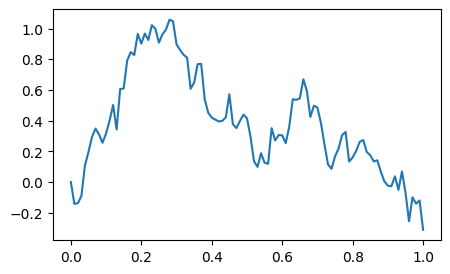
\includegraphics[width=7cm]{pic/bm-path.png}

Аналогичным образом можно симулировать сразу несколько траекторий.
Например, следующий фрагмент производит массив формы $(n+1, m)$, каждый столбец которого является одной траекторией геометрического броуновского движения с коэффициентом сноса $\mu$, волатильности $\sigma$ и начальным значением 1.
Мы воспользуется тем, что такой процесс является экспонентой броуновского движения со коэффициентом сноса $(mu-\frac12 sigma^2)$ и волатильности $\sigma$, и поэтому сначала будем симулировать траектории этого процесса, а затем применим функцию экспоненты. 
Следует обратить внимание на параметр \verb"axis=0", который используется для вычисления кумулятивной суммы приращений в каждом столбце по отдельности.

\begin{python}
### [numpy-basics.ipynb] ###
mu = 0
sigma = 1
m = 5

# Приращения всех траекторий броуновского движения со сносом
dX = rng.normal((mu - 0.5*sigma**2)*t/n, sigma*sqrt(t/n), (n, m))  
# Траектории броуновского движения со сносом
X = np.vstack((np.zeros(m), np.cumsum(dX, axis=0)))
# Траектории геометрического броуновского движения
S = np.exp(X)

# Если второй аргумент функции plot является 2-мерным массивом, то считается,
# что каждый столбец представляет собой отдельную функцию
plt.plot(T, S);
\end{python}

\noindent
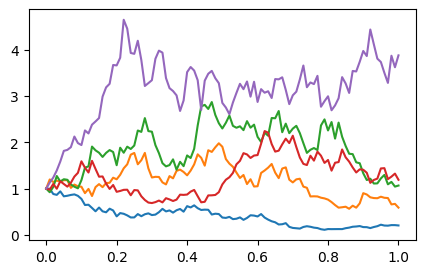
\includegraphics[width=7cm]{pic/gbm-paths.png}

%!TEX root=finmath1.tex
\chapter{Модель \crr}
\label{ch:pr-crr}
\chaptertoc

Здесь мы реализуем модель \crr\ и вычисление в ней цен европейских и американских платежных обязательств, а также метод симуляции траекторий цены рискового актива.
В последнем разделе обсудим приближение модели \bs\ с ее помощью.

\section{Принцип реализации моделей в виде классов}
При имплементации различных моделей часто бывает удобно объединить функции, относящиеся к одной модели.
В нашем курсе для этой цели будут использоваться классы Python. 
Модель (например, модель \crr) будет представлена классом, содержащим ее параметры и набор функций для вычисления цен деривативов, симуляции цен базового актива и \td\ 
Мы будем пользоваться \emph{датаклассами}, что позволяет сократить вспомогательный технический код.
\begin{python}
### crr.py ###
from dataclasses import dataclass, field
# ... [другие импорты]

@dataclass
class CoxRossRubinstein:
    s0: float
    u: float
    d: float
    r: float = 0.0
    q: float = field(init=False)   # q не инициализируется автоматически

    def __post_init__(self):
        # Вычисление риск-нейтральной вероятности
        self.q = (self.r - self.d) / (self.u - self.d)        
\end{python}

Декоратор \verb"@dataclass" "--- это удобная конструкция, которая автоматически добавляет в создаваемый класс конструктор, инициализирующий переменные, перечисленные в классе (для этого нужно указать все переменные и их типы).
Объект класса создается операцией \verb"model = CoxRossRubinstein(s0, u, d, r)".  

Использование датакласса удобно, например, тем, что не нужно писать стандартный код конструктора следующего вида.
\begin{python}
# В датаклассе такой конструктор будет создан автоматически
class CoxRossRubinstein:
    # ...
    def __init__(self, s0, u, d, r = 0.0):
      self.s0 = s0
      self.u = u
      self.d = d
      self.r = r
\end{python}

Метод \verb"__post_init__" будет вызван автоматически после завершения работы конструктора, и его можно использовать для инициализации аттрибутов класса, которые требуют вычислений.
В нашем классе таковой является риск-нейтральная вероятность \verb"q".
Чтобы она не была включена в конструктор, мы добавили \verb"field(init=False)" в ее определение.

В \verb"__post_init__" можно добавить также, например, проверку корректности параметров модели (но в пакете \verb"finmath1" такая проверка для простоты не осуществляется).
\begin{python}
class CoxRossRubinstein:
    # ...
    def __post_init__(self):
        if (self.u <= self.d) or (self.d <= -1):
            raise ValueError('Неверные параметры u, d')
        if not (self.d < self.r < self.u):
            raise ValueError('В модели присутствует арбитраж')
        # ...
\end{python}

Датаклассы предоставляют и другие удобные методы, имплементируемые автоматически: например, метод строкового представления \verb"__str__", производящий удобно читаемый вывод при использовании \verb"print(model)". 
\begin{python}
model = CoxRossRubinstein(100, 0.1, -0.1, 0.05)
print(model)  # CoxRossRubinstein(s0=100, u=0.1, d=-0.1, r=0.05, q=0.75)
\end{python}

\begin{remark}[как расширить функционал модели]
Модель \crr, реализованная в пакете \verb"finmath1", содержит лишь базовый функционал.
Если потребуется ее расширить для использования в каких-то других приложениях, то можно либо создать класс, производный от \verb"CoxRossRubinstein" и содержащий новые функции, либо добавить глобальные функции, принимающие объект класса \verb"CoxRossRubinstein" в качестве аргумента.
То же самое относится и к другим моделям пакета. 
\begin{python}
# Производный класс от CoxRossRubinstein
class CoxRossRubinsteinExtended(CoxRossRubinstein):
    def new_function(self, arg1, arg2, ...):
    # ...

# Глобальная функции
def new_function(model, arg1, arg2, ...):
    # ...

# Использование функции из производного класса
model = CoxRossRubinsteinExtended(s0=100, u=0.1, d=0.1, r=0.05)
result = model.new_function(arg1, arg2, ...)

# Использование глобальной функции
model = CoxRossRubinstein(s0=100, u=0.1, d=0.1, r=0.05)
result = new_function(model, arg1, arg2, ...)
\end{python}
\end{remark}


\section{Вычисление цен платежных обязательств}
\subsection{Европейские обязательства, не зависящие от траектории}
Реализуем функцию вычисления цены в момент $t=0$ для европейского платежного обязательства, не зависящего от траектории цены рискового актива. Напомним, что такое платежное обязательство имеет вид $X=f(S_T)$.

Согласно результату из лекции \ref{ch:crr}, его цену можно представить в виде математического ожидания функции от случайной величины, равной количеству <<шагов вверх>> цены рискового актива и имеющей биномиальное распределение с параметрами $(T,q)$ относительно риск-нейтральной вероятности:
\[
V_0^X = \frac{1}{(1+r)^T}\E^\Q X = \frac{1}{(1+r)^T} \sum_{n=0}^T f\bigl(S_0(1+u)^n(1+d)^{T-n}\bigr) C_T^n q^n (1-q)^{T-n}.
\]

Реализуемая ниже функция цены имеет два аргумента\footnote{Помимо аргумента \verb"self".}: скалярный аргумент \verb"maturity" задает время исполнения, а аргумент \verb"payoff" должен быть универсальной функцией, которая, будучи примененной к массиву значений цены рискового актива в момент $T=$\;\verb"maturity", возвращает массив значений $f(S_T)$. 
\begin{python}
### crr.py ###
class CoxRossRubinstein:
    # ...
    def path_indep_price(self, maturity, payoff):
        N = np.arange(maturity+1)
        Q = comb(maturity, N) * self.q**N * (1-self.q)**N[::-1]
        S = self.s0 * (1+self.u)**N * (1+self.d)**N[::-1]
        return np.dot(Q, payoff(S)) / (1+self.r)**maturity
\end{python}

В этой функции массив \verb"S" содержит всевозможные значения цены рискового актива в момент $T=$\;\verb"maturity", а массив \verb"Q" "--- риск-нейтральные вероятности, что цена примет соответствущие значения.
Оба массива имеют длину \verb"maturity+1", а их $n$-ые элементы соответствуют случайному событию, когда цена идет вверх ровно $n$ раз.
Функция \verb"comb" из пакета \verb"scipy.special" вычисляет массив биномиальных коэффициентов. 
Массив \verb"payoff(S)" содержит значения выплаты $X$.
Умножая его скалярно на \verb"Q" с помощью функции \verb"np.dot", получается математическое ожидание $\E^\Q X$, которое потом дисконтируется.

Заметим, что \verb"payoff(S)" может быть и многомерным массивом, если в качестве $X$ выступает массив платежных обязательств.
Чтобы \verb"path_indep_price" в таком случае корректно работала при вычислении скалярного произведения%
\footnote{Функция \verb"np.dot(x, y)", примененная к одномерному массиву \verb"x" и многомерному массиву \verb"y", возвращает сумму произведений значений \verb"x[n]" на срезы \verb"y[n]".},
каждый срез \verb"payoff(S)[n]" должен содержать значения выплат всех платежных обязательств на случайном событии, когда цена идет вверх ровно $n$ раз. Соответственно, длина массива \verb"payoff(S)" по оси 0 должна совпадать с длиной \verb"P".
Например, если \verb"payoff(S)" "--- двумерный массив, то его $n$-я строка будет содержать значения всех выплат в случае, когда цена рискового актива идет вверх $n$ раз (платежные обязательства в таком случае образуют одномерный массив).

Используя функцию \verb"path_indep_price", добавим в наш класс методы для вычисления цен европейских опционов колл и пут.
\begin{python}
### crr.py ###
class CoxRossRubinstein:
    # ...
    def call_price(self, maturity, strike):
        payoff = lambda s: np.maximum(np.subtract.outer(s, strike), 0)
        return self.path_indep_price(maturity, payoff)
    
    def put_price(self, maturity, strike):
        payoff = lambda s: np.maximum(-np.subtract.outer(s, strike), 0)
        return self.path_indep_price(maturity, payoff)
\end{python}
Здесь считается, что аргумент \verb"maturity" является скаляром, а \verb"strike" может быть как скаляром, так и одномерным массивом\footnote{Функция будет работать и для многомерного массива \verb"strike", но трудно представить, где это может потребоваться.}.
Использование массива страйков позволяет вычислить цены сразу всех нужных опционов для заданного времени исполнения.
Это удобно и, главное, быстрее, чем вычислять цены по отдельности в дополнительном цикле.

Заметим, что для задания выплаты опциона создается лямбда-функция\footnote{Лямбда-функция "--- это безымянная функция; такие функции удобно использовать в промежуточных вычислениях.}, передаваемая в \verb"path_indep_price".
В этой функции мы пользуемся операцией внешнего вычитания, которая позволяет корректно учитывать как случай скалярного страйка, так и массива страйков.
А именно, если \verb"strike" "--- массив, то вычитание его из массива значений цены рискового актива \verb"s" дает двумерный массив, каждая строка которого состоит из всех значений выплаты опциона колл с соответствущим страйком.
Для опциона пут аналогичное поведение достигается сменой знака (написать \verb"np.subtract.outer(strike ,s)" нельзя, так как получатся несогласованные размерности).
В итоге, \verb"path_indep_price" возвращает одномерный массив с ценами всех опционов для различных страйков.

В качестве примера, вычислим цену опциона колл из примера \ref{crr:example} в лекции \ref{ch:crr}, а также массив цен трех опционов в той же модели.
\begin{python}
### crr.ipynb ###
model = CoxRossRubinstein(s0=100, u=0.1, d=-0.1, r=0.05)
print(model.call_price(2, 100))             # 10.71
print(model.call_price(2, [90, 100, 110]))  # [18.88, 10.71, 5.61]
print(model.put_price(2, [90, 100, 110]))   # [0.51, 1.42, 5.39]
\end{python}


\subsection{Европейские обязательства, зависящие от траектории}
\label{pr-crr:s:path-dep}
Рассмотрим теперь платежное обязательство вида $X = f(S_0,\dots,S_T)$, зависящее от траектории цены рискового актива. 
Для вычисления его цены воспользуемся формулой
\[
V_0^X = \frac1{(1+r)^T} \E^{\Q} X = \frac1{(1+r)^T} \sum_{\omega\in\Omega} f(S_0, S_1(\omega),\dots,S_T(\omega)) \Q(\omega).
\]
Чтобы вычислить сумму, создадим массив всех исходов \verb"Omega", массив выплат \verb"X", соответствующих этим исходам, и массив \verb"Q" их вероятностей; затем перемножим \verb"X" и \verb"Q", дисконтируем и получим искомую цену.
Приведем сначала всю функцию, а потом поясним, как она работает.
\begin{python}
### crr.py ###
class CoxRossRubinstein:
    # ...
    def path_dep_price(self, maturity, payoff):
        Omega = np.unpackbits(np.arange(2**maturity, dtype='<u8').view('u1').\
            reshape((-1, 8)), axis=1, count=maturity, bitorder='little').T
        Q  = (self.q/(1-self.q))**np.sum(Omega, axis=0) * (1-self.q)**maturity
        xi = np.where(Omega, 1+self.u, 1+self.d)
        S = self.s0*np.vstack((np.ones(2**maturity), np.cumprod(xi, axis=0)))
        X = payoff(S)
        return np.dot(Q, X) / (1+self.r)**maturity
\end{python}

Здесь каждый столбец двумерного массива \verb"Omega" содержит двоичное представление одного случайного исхода, \te\ \verb"Omega[t, n]" равно 0 или 1 в зависимости от того, идет ли цена вниз или вверх на шаге $t$ при $n$-м случайном исходе.
В частности, \verb"Omega" имеет форму $(T,\, 2^T)$, где $T=$\;\verb"maturity".

Для создания массива \verb"Omega" применяется несколько нетривиальная, но эффективная процедура, состоящая в следующем.
Сначала функция \verb"np.arange" создает массив чисел от 0 до $2^T-1$, причем ее аргумент \verb"dtype='<u8'" означает, что каждый элемент этого массива должен храниться в оперативной памяти как 8-байтное неотрицательное целое число с порядком байтов от младшего к старшему\footnote{Например, число 1 будет представлено в виде последовательности байтов $1,0,0,0,0,0,0,0$, а 258 "--- в виде $2,1,0,0,0,0,0,0$ (так называемый \emph{little-endian} порядок байтов, см.\ \url{https://en.wikipedia.org/wiki/Endianness}).}.
Затем метод \verb"view" <<разворачивает>> каждый элемент в 8 однобайтных элементов, таким образом увеличивая длину массива в 8 раз.
Потом применяется \verb"reshape", делая массив двумерным, так что каждая его строка содержит 8 однобайтных чисел (и тогда строка $n$ представляет число $n$).
К полученному массиву применяется функция \verb"np.unpackbits", которая преобразует каждый элемент массива в 8 новых элементов со значениями 0 или 1 и содержащие его биты.
Аргумент \verb"axis=1" означает, что нужно работать по строкам: битовые представления чисел в каждой строке исходного массива будут записаны в соответствующую строку нового массива, а количество строк в массиве останется прежним. 
Аргумент \verb"bitorder='little'" указывает, что биты должны идти от младшего к старшему, а \verb"count=maturity" оставляет в каждой строке нового массива только только первые \verb"maturity" элементов.
Наконец, полученный массив транспонируется, чтобы представление числа $n$ было записано в столбце $n$.

\begin{remark}
Функция \verb"np.unpackbits" работает только с массивами, элементами которых является целые однобайтные числа, и именно поэтому нам пришлось вызывать дополнительно \verb"view" и \verb"reshape", вместо того, чтобы написать что-то вроде \verb"np.unpackbits(np.arange(2**maturity), count=maturity)".
\end{remark}

Далее для вычисления массива вероятностей $Q$ используется формула
\[
\Q(\omega) = \left(\frac{1+u}{1+d}\right)^{\sum_{n=1}^T a_n} (1+d)^T,
\]
где каждый исход $\omega=(a_1,\dots,a_T)$ соответствует одному столбцу массива \verb"Omega", и поэтому при вычислении суммы мы указываем аргумент \verb"axis=0", суммирующий по строкам.

Массив \verb"xi" получается из \verb"Omega" заменой 0 на $1+d$, а 1 на $1+u$, для чего используется функция \verb"np.where".
В общем случае \verb"np.where(x, a, b)" принимает массив логических значений \verb"x" и возвращает массив такой же формы, где на месте каждого истинного значения записано \verb"a", а на месте ложного "--- \verb"b" (при этом \verb"a" и \verb"b" могут быть массивами, тогда из них будут выбираться элементы с соответствующими индексами; подробнее см.~документацию\footnote{\url{https://numpy.org/doc/2.2/reference/generated/numpy.where.html}}).
В нашем случае нулевые элементы \verb"Omega" трактуются как ложные, а единичные как истинные. 

Двумерный массив \verb"S" в каждом своем столбце содержит траекторию цены рискового актива (и, следовательно, имеет форму $(T+1,\, 2^T)$).
Для его создания используется формула
\[
S_0 = s_0, \qquad S_t = S_{t-1}\xi_t,\ t=1,\dots,T,
\]
вычисление которой выполняется применением функции кумулятивного произведения вдоль столбцов массива \verb"xi", добавлением сверху строки из единиц и умножением на начальное условие. 

Массив выплат \verb"X" получается применением передаваемой функции \verb"payoff" к \verb"S". Считается, что она возвращает одномерный массив, состоящий из значений выплаты платежного обязательства на каждой траектории%
\footnote{Все будет работать и в случае нескольких платежных обязательств.
Тогда \verb"payoff" должна возвращать многомерный массив, у которого каждый срез \verb"payoff(S)[n]" представляет значения выплат всех платежных обязательств на траектории $S(\omega_n)$.}.

Наконец, массив вероятностей умножается на массив выплат, что дает математическое ожидание $\E^{\Q} X$, которое потом дисконтируется.

Проверим работу реализованного алгоритма сначала на каком-нибудь простом случае.
В качестве примера, вычислим с его помощью цену опциона колл из предыдущего раздела.
\begin{python}
model = CoxRossRubinstein(s0=100, u=0.1, d=-0.1, r=0.05)
print(model.path_dep_price(2, lambda s: np.maximum(s[-1] - 100, 0)))  # 10.71
\end{python}
Здесь функция выплаты устроена так, что из массива траекторий цены рискового актива она берет только последнюю строку (значения $S_T$) и вычисляет выплату опциона колл со страйком 100.
Получается тот же результат, что и при использовании \verb"path_indep_price" и \verb"call_price".

Теперь приведем более содержательный пример и вычислим цену барьерного опциона вниз-и-выход из примера \ref{crr:e:barrier} в лекции \ref{ch:crr}.
\begin{python}
### crr.ipynb ##
T = 2
K = 95
H = 92
barrier_payoff = lambda s: np.maximum(s[-1] - K, 0) * np.all(s>=H, axis=0)
print(model.path_dep_price(T, barrier_payoff))  # 13.95
\end{python}
Здесь выплата опциона колл умножается на индикатор того, что цена находилась не ниже барьера $H$.
Заметим, что выражение \verb"s>=H" является массивом (такой же формы как \verb"s") и содержит значения \verb"True" или \verb"False" в зависимости от того, находится ли каждое значение цены не ниже барьера.
Функция \verb"np.all" реализует операцию логического <<и>>.
В данном случае она применяется по строкам (\verb"axis=0"), \te\ получается одномерный массив, каждый элемент которого будет равен \verb"True", если все элементы соответствующего столбца массива \verb"s>=H" истинны, и \verb"False" иначе.
При умножении числового массива \verb"np.maximum(s[-1] - K, 0)" на получившийся логический массив значение \verb"True" трактуется как 1, а \verb"False" как 0, что и соответствует умножению на индикатор.

\begin{remark}
Представление выплат сложных деривативов в виде универсальной функции может быть иногда затруднительно.
Вместо этого можно написать функцию выплаты, применяемую к одной траектории, а в \verb"path_dep_price" передать лямбда-функцию, которая будет применять ее к каждому столбу передаваемого двумерного массива цен (хотя это приведет к потере скорости).

Например, предыдущий фрагмент можно было бы переписать следующим образом.
\begin{python}
barrier_payoff = lambda s: max(s[-1] - K, 0) * np.all(s>=H)
print(model.path_dep_price(T, lambda S : [barrier_payoff(s) for s in S.T]))
\end{python}
Здесь считается, что в \verb"barrier_payoff" передается одномерный массив \verb"s", а поэтому \verb"s[-1] - K" является скаляром, и можно воспользоваться встроенной функцией \verb"max" вместо \verb"np.maximum".
Кроме того, не нужно указывать \verb"axis=0" при вызове \verb"np.all". 
Далее при вызове \verb"path_dep_price" создается лямбда-функция, которая применяет функцию выплаты к каждому столбцу передаваемого двумерного массива \verb"S" (конструкция \verb"s in ..." проходит по строкам массива, а так как нам нужны столбцы, то нужно транспонировать \verb"S").
\end{remark}


\subsection{Американские обязательства}
Для вычисления цен американских платежных обязательств воспользуемся методом обратной индукции.
Мы будем рассматривать платежные обязательства, выплата которых при исполнении в момент времени $t$ зависит только от цены базового акива в этот момент, т.е.\ $X_t=f(S_t)$, где $f(s)$ "--- детерминированная функция.
Такой вид, в частности, имеют функции выплат американских опционов колл и пут.
\begin{python}
### crr.py ###
class CoxRossRubinstein:
    # ...
    def american_price(self, maturity, payoff):
        def X(t):
            N = np.arange(t+1)
            return payoff(self.s0 * (1+self.u)**N * (1+self.d)**(t-N))
        V = X(maturity)
        for t in range(maturity-1, -1, -1): # t пробегает от maturity-1 до 0
            V[:t+1] = np.maximum(X(t),
                (self.q*V[1:t+2] + (1-self.q)*V[:t+1])/(1+self.r))
        return V[0]    
\end{python}
Сначала здесь создается вспомогательная функция \verb"X", вычисляющая массив всех возможных значений выплаты $X_t$.
Предполагается, что \verb"payoff", играющая роль указанной выше функции $f$, является универсальной функцией, которая применяется к массиву значений цены базового актива и возвращает соответствующий массив значений выплат платежного обязательства. 

Далее реализуется собственно алгоритм обратной индукции.
Мы пользуемся тем, что, в силу марковского свойства цены базового актива, справедливо равенство $V_{t} = V(t, S_{t})$, где функция $V(t,s)$ имеет вид
\begin{align*}
&V(T, s) = f(s), \\
&V(t, s) = \max(f(s),\ (1+r)^{-1}\E^\Q(V({t+1}, S_{t+1}) \mid S_t=s))\ \text{при}\ t < T,
\end{align*}
причем присутствующее здесь условное математическое ожидание можно вычислить по формуле
\[
\E^\Q(V({t+1}, S_{t+1}) \mid S_t=s) = qV(t+1, s(1+u)) + (1-q)V(t+1, s(1+d)).
\]
По ходу обратной индукции значения функции $V(t,s)$ на шаге $t=T,T-1,\dots,0$ записываются в массив \verb"V", перезаписывая его первые $t+1$ элементов, так что элемент \verb"V[n]", где $n=0,\dots,t$, представляет значение функции $V(t, s)$ для $s=s_0(1+u)^n(1+d)^{t-n}$.
Искомое значение цены в начальный момент времени будет записано в \verb"V[0]" на последнем шаге цикла.

Используя написанную общую функцию, добавим в класс также методы вычисления цен американских опционов колл и пут (в этих функциях предполагается, что оба аргумента \verb"maturity" и \verb"strike" являются скалярами).
\begin{python}
### crr.py ###
class CoxRossRubinstein:
    # ...
    def american_call_price(self, maturity, strike):
        return self.american_price(lambda s: np.maximum(s-strike, 0), maturity)

    def american_put_price(self, maturity, strike):
        return self.american_price(lambda s: np.maximum(strike-s, 0), maturity)
\end{python}

В качестве иллюстрации, найдем цену американских опционов колл и пут со страйком $K=102$ для двухшаговой модели приведенной выше (цену пут мы нашли в примере \ref{am-d:e:price} в лекции \ref{ch:american-discrete}).
Заметим, что цена американского опциона колл совпадает с ценой европейского опциона колл, как и должно быть при неотрицательной процентной ставке в отсутствие дивидендов, см.~раздел \ref{am-d:s:equal-prices} в лекции \ref{ch:american-discrete}.
Цены опционов пут различаются.
\begin{python}
### crr.ipynb ###
print(model.american_call_price(2, 102))  # 9.69 (американский колл)
print(model.call_price(2, 102))           # 9.69 (европейский колл)
print(model.american_put_price(2, 102))   # 3.37 (американский пут)
print(model.put_price(2, 102))            # 2.21 (европейский пут)
\end{python}


\section{Симуляция цены рискового актива}
Реализуем функцию, симулирующую траектории цены рискового актива, чтобы использовать их, например, в методе \mc.
Так как гораздо эффективнее симулировать траектории не по одной, а группами (чтобы использовать векторизацию), то нам нужна функция, возвращающая двумерный массив из заданного количества траекторий.
Везде далее будет предполагаться, что одна траектория представлена столбцом этого массива, и, таким образом, массив должен иметь форму $(T+1, M)$, где $M$ "--- требуемое количество траекторий.
Мы включаем в каждую траекторию начальное значение $S_0$, поэтому число строк в массиве равно $T+1$.

Траектории всегда будут симулироваться относительно риск-нейтральной вероятности. 
Воспользуемся тем, что относительно нее справедливо представление
\[
S_t = S_{t-1}\xi_t,
\]
где $\xi_1,\dots,\xi_T$ "--- независимые случайные величины, принимающие значения $1+u$ и $1+d$ с вероятностями $q$ и $1-q$.

\begin{python}
### crr.py ###
class CoxRossRubinstein:
    # ...
    def simulate(self, t, paths, rng=None):
        if rng is None:
            rng = np.random.default_rng()  
        xi = np.where(rng.uniform(size=(t, paths)) < self.q, 1+self.u, 1+self.d)
        return self.s0*np.vstack((np.ones(paths), np.cumprod(xi, axis=0)))
\end{python}
Эта функция принимает целочисленные аргументы \verb"t" (последний момент времени) и \verb"paths" (количество траекторий), а также объект генератора случайных чисел 
\verb"rng". Если \verb"rng" равен \py{None}, то будет использован генератор по умолчанию.
Если нужна воспроизводимость результатов, то следует передать заранее созданный генератор с фиксированным начальным состоянием (см.~замечание \ref{np:r:seed} в практикуме \ref{ch:numpy}).

Массив \verb"xi" составлен из столбцов, содержащих значения $\xi_1,\dots,\xi_T$ для каждой симулированной траектории: \verb"rng.uniform(size=(t, paths)) < self.q" дает двумерный массив, составленный из значений \verb"True" или \verb"False" с вероятностями $q$ и $1-q$, а затем к нему применяется функция выбора \verb"np.where" подобно тому, как это делалось разделе \ref{pr-crr:s:path-dep}.
Из массива \verb"xi" получается массив траекторий цен, опять же, аналогично коду в разделе \ref{pr-crr:s:path-dep}.

В качестве примера, приводимый ниже фрагмент кода симулирует небольшое число траекторий и строит их графики.
В следующем практикуме мы увидим, как пользоваться этой функцией в методе \mc.
\begin{python}
### crr.ipynb ###
# 5 траекторий в 50-шаговой модели
model = CoxRossRubinstein(s0=100, u=0.02, d=-0.02)
plt.plot(model.simulate(50, 5))
plt.xticks(range(0, 51, 10));  # Сделать отметки по оси x через каждые 10 шагов
\end{python}

\noindent
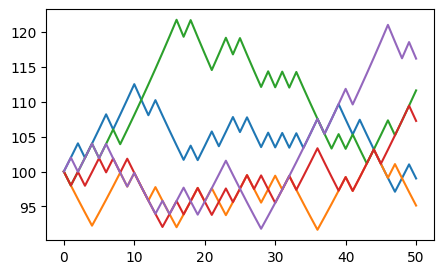
\includegraphics[width=7cm]{pic/crr-path-many.png}


\section{Приближение модели \bs}
Как показано в дополнительном материале \ref{ch:crr-limit}, модель \crr\ сходится к модели \bs\ при числе шагов $T\to\infty$ и параметрах $u,d,r\to0$, и, в частности, сходятся цены платежных обязательств (при некоторых условиях на интегрируемость функции выплат).
Продемонстрируем это на примере сходимости цен европейских опционов колл.

Рассмотрим модель \bs\ с фиксированными параметрами $s_0$, $\sigma$, $r$ и модель \crr\ такой же начальной ценой $s_0$ и параметрами
\[
u = \frac{\sigma}{\sqrt n}, \qquad d = -\frac{\sigma}{\sqrt n}, \qquad r' = \frac{r}{n}.
\]
Построим графики цен опционов колл с моментом исполнения $T$ в модели \bs\ и моментом исполнения $Tn$ в модели \crr, где $T$ "--- <<календарное>> время (чтобы избежать дополнительных трудностей с округлением, будем считать, что $T$ "--- целое), а также построим графики их подразумеваемой волатильности (см.~замечание ниже о том, зачем это делать).
Следующий фрагмент кода иллюстрирует это для $n=10$ и $n=100$.
В нем используется класс \verb"BlackScholes", а также функция вычисления подразумеваемой волатильности \verb"implied_vol", которые будут разбираться в дальнейших практикумах.
\begin{python}
### crr.ipynb ###
s0 = 100
sigma = 0.3
r = 0.05
T = 1

# Создадим 4 подграфика и отрегулируем горизонтальный промежуток между ними
fig, ax = plt.subplots(2, 2, figsize=(10,6), squeeze=False)
fig.subplots_adjust(hspace=0.4)

# Модель Блэка-Шоулса и цены опционов в ней
bs_model = BlackScholes(s0, sigma, r)     
K = np.linspace(50, 200, 100)   # диапазон страйков
bs_price = bs_model.call_price(T, K)

for i, n in enumerate([10, 100]):
    # Цены опционов и их волатильность в модели Кокса-Росса-Рубинштейна
    crr_model = CoxRossRubinstein(s0, sigma/sqrt(n), -sigma/sqrt(n), r/n)
    crr_price = crr_model.call_price(T*n, K)
    crr_iv = implied_vol(s0*exp(r*T), T, K, crr_price, discount_factor=exp(-r*T))

    # Слева будут графики цен
    ax[i,0].plot(K, bs_price, label="Блэк-Шоулс")
    ax[i,0].plot(K, crr_price, label="Кокс-Росс-Рубинштейн")
    ax[i,0].legend(loc="upper right", frameon=False)
    ax[i,0].set_title(f"Цены опционов (n={n})", fontsize=10, fontweight="bold")
    ax[i,0].set_xlabel("Страйк")
    ax[i,0].set_ylabel("Цена")

    # а справа - графики волатильности
    ax[i,1].plot(K, np.ones(len(K))*sigma, label="Блэк-Шоулс")
    ax[i,1].plot(K, crr_iv, label="Кокс-Росс-Рубинштейн")
    ax[i,1].set_ylim(0.25, 0.35)
    ax[i,1].legend(loc="upper right", frameon=False)
    ax[i,1].set_title(f"Подразумеваемая волатильность (n={n})", fontsize=10,
        fontweight="bold")
    ax[i,1].set_xlabel("Страйк")
    ax[i,1].set_ylabel("Волатильность")
\end{python}

\noindent
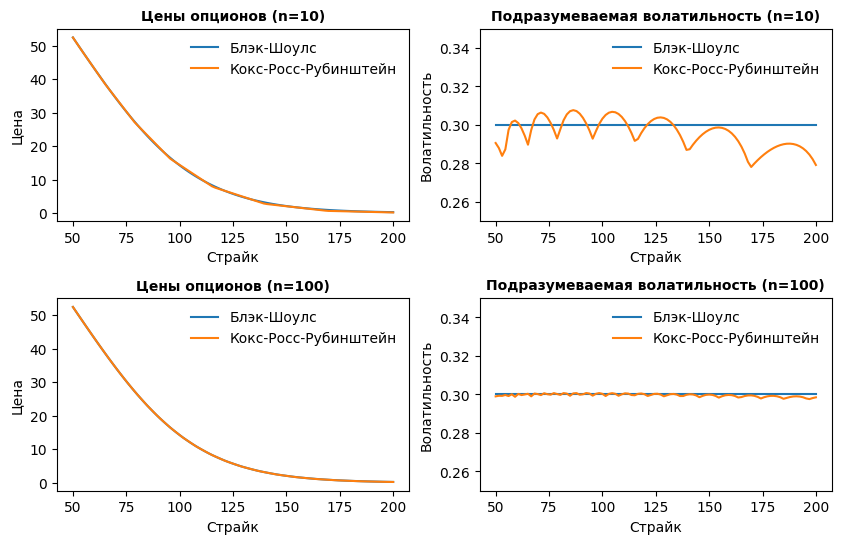
\includegraphics[width=14cm]{pic/crr-limit.png}

\begin{remark}
Мы приводим графики подразумеваемой волатильности потому, что она позволяет лучше понять, насколько качественным является построенное приближение.
На графиках видно, что цены опционов для модели \crr\ и \bs\ близки и при $n=10$, и при $n=100$, но при $n=10$ приближение волатильности получается недостаточно хорошим (ошибка около 2\%, которая здесь получается, на практике не считается пренебрежительной).
\end{remark}

%\printindex

\clearpage
\titlecontents{chapter}[0em]{}{}{}{\dotfill\contentspage}
\phantomsection
\addtocontents{toc}{\vspace{1em}}
\chapter*{Список литературы}
\addcontentsline{toc}{chapter}{\textbf{Список литературы}}

\defbibheading{main}{\section*{Основные источники}}
\defbibheading{aux}{\section*{Дополнительные источники}}
\printbibliography[keyword=fm1-main,heading=main]
\printbibliography[notkeyword=fm1-main,heading=aux]

\end{document}
